%
% This is an example LaTeX file which uses the SANDreport class file.
% It shows how a SAND report should be formatted, what sections and
% elements it should contain, and how to use the SANDreport class.
% It uses the LaTeX article class, but not the strict option.
% ItINLreport uses .eps logos and files to show how pdflatex can be used
%
% Get the latest version of the class file and more at
%    http://www.cs.sandia.gov/~rolf/SANDreport
%
% This file and the SANDreport.cls file are based on information
% contained in "Guide to Preparing {SAND} Reports", Sand98-0730, edited
% by Tamara K. Locke, and the newer "Guide to Preparing SAND Reports and
% Other Communication Products", SAND2002-2068P.
% Please send corrections and suggestions for improvements to
% Rolf Riesen, Org. 9223, MS 1110, rolf@cs.sandia.gov
%
\documentclass[pdf,12pt]{INLreport}
% pslatex is really old (1994).  It attempts to merge the times and mathptm packages.
% My opinion is that it produces a really bad looking math font.  So why are we using it?
% If you just want to change the text font, you should just \usepackage{times}.
% \usepackage{pslatex}
\usepackage{times}
\usepackage[FIGBOTCAP,normal,bf,tight]{subfigure}
\usepackage{amsmath}
\usepackage{amssymb}
\usepackage{pifont}
\usepackage{enumerate}
\usepackage{listings}
\usepackage{fullpage}
\usepackage{xcolor}          % Using xcolor for more robust color specification
\usepackage{ifthen}          % For simple checking in newcommand blocks
\usepackage{textcomp}
%\usepackage{authblk}         % For making the author list look prettier
%\renewcommand\Authsep{,~\,}

% Custom colors
\definecolor{deepblue}{rgb}{0,0,0.5}
\definecolor{deepred}{rgb}{0.6,0,0}
\definecolor{deepgreen}{rgb}{0,0.5,0}
\definecolor{forestgreen}{RGB}{34,139,34}
\definecolor{orangered}{RGB}{239,134,64}
\definecolor{darkblue}{rgb}{0.0,0.0,0.6}
\definecolor{gray}{rgb}{0.4,0.4,0.4}

\lstset {
  basicstyle=\ttfamily,
  frame=single
}

\setcounter{secnumdepth}{5}
\lstdefinestyle{XML} {
    language=XML,
    extendedchars=true, 
    breaklines=true,
    breakatwhitespace=true,
%    emph={name,dim,interactive,overwrite},
    emphstyle=\color{red},
    basicstyle=\ttfamily,
%    columns=fullflexible,
    commentstyle=\color{gray}\upshape,
    morestring=[b]",
    morecomment=[s]{<?}{?>},
    morecomment=[s][\color{forestgreen}]{<!--}{-->},
    keywordstyle=\color{cyan},
    stringstyle=\ttfamily\color{black},
    tagstyle=\color{darkblue}\bf\ttfamily,
    morekeywords={name,type},
%    morekeywords={name,attribute,source,variables,version,type,release,x,z,y,xlabel,ylabel,how,text,param1,param2,color,label},
}
\lstset{language=python,upquote=true}

\usepackage{titlesec}
\newcommand{\sectionbreak}{\clearpage}
\setcounter{secnumdepth}{4}

%\titleformat{\paragraph}
%{\normalfont\normalsize\bfseries}{\theparagraph}{1em}{}
%\titlespacing*{\paragraph}
%{0pt}{3.25ex plus 1ex minus .2ex}{1.5ex plus .2ex}

%%%%%%%% Begin comands definition to input python code into document
\usepackage[utf8]{inputenc}

% Default fixed font does not support bold face
\DeclareFixedFont{\ttb}{T1}{txtt}{bx}{n}{9} % for bold
\DeclareFixedFont{\ttm}{T1}{txtt}{m}{n}{9}  % for normal

\usepackage{listings}

% Python style for highlighting
\newcommand\pythonstyle{\lstset{
language=Python,
basicstyle=\ttm,
otherkeywords={self, none, return},             % Add keywords here
keywordstyle=\ttb\color{deepblue},
emph={MyClass,__init__},          % Custom highlighting
emphstyle=\ttb\color{deepred},    % Custom highlighting style
stringstyle=\color{deepgreen},
frame=tb,                         % Any extra options here
showstringspaces=false            % 
}}


% Python environment
\lstnewenvironment{python}[1][]
{
\pythonstyle
\lstset{#1}
}
{}

% Python for external files
\newcommand\pythonexternal[2][]{{
\pythonstyle
\lstinputlisting[#1]{#2}}}

\lstnewenvironment{xml}
{}
{}

% Python for inline
\newcommand\pythoninline[1]{{\pythonstyle\lstinline!#1!}}

% Named Colors for the comments below (Attempted to match git symbol colors)
\definecolor{RScolor}{HTML}{8EB361}  % Sonat (adjusted for clarity)
\definecolor{DPMcolor}{HTML}{E28B8D} % Dan
\definecolor{JCcolor}{HTML}{82A8D9}  % Josh (adjusted for clarity)
\definecolor{AAcolor}{HTML}{8D7F44}  % Andrea
\definecolor{CRcolor}{HTML}{AC39CE}  % Cristian
\definecolor{RKcolor}{HTML}{3ECC8D}  % Bob (adjusted for clarity)
\definecolor{DMcolor}{HTML}{276605}  % Diego (adjusted for clarity)
\definecolor{PTcolor}{HTML}{990000}  % Paul

\def\DRAFT{} % Uncomment this if you want to see the notes people have been adding
% Comment command for developers (Should only be used under active development)
\ifdefined\DRAFT
  \newcommand{\nameLabeler}[3]{\textcolor{#2}{[[#1: #3]]}}
\else
  \newcommand{\nameLabeler}[3]{}
\fi
\newcommand{\alfoa}[1] {\nameLabeler{Andrea}{AAcolor}{#1}}
\newcommand{\cristr}[1] {\nameLabeler{Cristian}{CRcolor}{#1}}
\newcommand{\mandd}[1] {\nameLabeler{Diego}{DMcolor}{#1}}
\newcommand{\maljdan}[1] {\nameLabeler{Dan}{DPMcolor}{#1}}
\newcommand{\cogljj}[1] {\nameLabeler{Josh}{JCcolor}{#1}}
\newcommand{\bobk}[1] {\nameLabeler{Bob}{RKcolor}{#1}}
\newcommand{\senrs}[1] {\nameLabeler{Sonat}{RScolor}{#1}}
\newcommand{\talbpaul}[1] {\nameLabeler{Paul}{PTcolor}{#1}}
% Commands for making the LaTeX a bit more uniform and cleaner
\newcommand{\TODO}[1]    {\textcolor{red}{\textit{(#1)}}}
\newcommand{\xmlAttrRequired}[1] {\textcolor{red}{\textbf{\texttt{#1}}}}
\newcommand{\xmlAttr}[1] {\textcolor{cyan}{\textbf{\texttt{#1}}}}
\newcommand{\xmlNodeRequired}[1] {\textcolor{deepblue}{\textbf{\texttt{<#1>}}}}
\newcommand{\xmlNode}[1] {\textcolor{darkblue}{\textbf{\texttt{<#1>}}}}
\newcommand{\xmlString}[1] {\textcolor{black}{\textbf{\texttt{'#1'}}}}
\newcommand{\xmlDesc}[1] {\textbf{\textit{#1}}} % Maybe a misnomer, but I am
                                                % using this to detail the data
                                                % type and necessity of an XML
                                                % node or attribute,
                                                % xmlDesc = XML description
\newcommand{\default}[1]{~\\*\textit{Default: #1}}
\newcommand{\nb} {\textcolor{deepgreen}{\textbf{~Note:}}~}


%%%%%%%% End comands definition to input python code into document

%\usepackage[dvips,light,first,bottomafter]{draftcopy}
%\draftcopyName{Sample, contains no OUO}{70}
%\draftcopyName{Draft}{300}

% The bm package provides \bm for bold math fonts.  Apparently
% \boldsymbol, which I used to always use, is now considered
% obsolete.  Also, \boldsymbol doesn't even seem to work with
% the fonts used in this particular document...
\usepackage{bm}

% Define tensors to be in bold math font.
\newcommand{\tensor}[1]{{\bm{#1}}}

% Override the formatting used by \vec.  Instead of a little arrow
% over the letter, this creates a bold character.
\renewcommand{\vec}{\bm}

% Define unit vector notation.  If you don't override the
% behavior of \vec, you probably want to use the second one.
\newcommand{\unit}[1]{\hat{\bm{#1}}}
% \newcommand{\unit}[1]{\hat{#1}}

% Use this to refer to a single component of a unit vector.
\newcommand{\scalarunit}[1]{\hat{#1}}

% \toprule, \midrule, \bottomrule for tables
\usepackage{booktabs}

% \llbracket, \rrbracket
\usepackage{stmaryrd}

\usepackage{hyperref}
\hypersetup{
    colorlinks,
    citecolor=black,
    filecolor=black,
    linkcolor=black,
    urlcolor=black
}

% Compress lists of citations like [33,34,35,36,37] to [33-37]
\usepackage{cite}

% If you want to relax some of the SAND98-0730 requirements, use the "relax"
% option. It adds spaces and boldface in the table of contents, and does not
% force the page layout sizes.
% e.g. \documentclass[relax,12pt]{SANDreport}
%
% You can also use the "strict" option, which applies even more of the
% SAND98-0730 guidelines. It gets rid of section numbers which are often
% useful; e.g. \documentclass[strict]{SANDreport}

% The INLreport class uses \flushbottom formatting by default (since
% it's intended to be two-sided document).  \flushbottom causes
% additional space to be inserted both before and after paragraphs so
% that no matter how much text is actually available, it fills up the
% page from top to bottom.  My feeling is that \raggedbottom looks much
% better, primarily because most people will view the report
% electronically and not in a two-sided printed format where some argue
% \raggedbottom looks worse.  If we really want to have the original
% behavior, we can comment out this line...
\raggedbottom
\setcounter{secnumdepth}{5} % show 5 levels of subsection
\setcounter{tocdepth}{5} % include 5 levels of subsection in table of contents

% ---------------------------------------------------------------------------- %
%
% Set the title, author, and date
%
\title{RAVEN User Manual}
%\author{%
%\begin{tabular}{c} Author 1 \\ University1 \\ Mail1 \\ \\
%Author 3 \\ University3 \\ Mail3 \end{tabular} \and
%\begin{tabular}{c} Author 2 \\ University2 \\ Mail2 \\ \\
%Author 4 \\ University4 \\ Mail4\\
%\end{tabular} }


\author{
\textbf{\textit{Principal Investigator (PI):}}
 \\Cristian Rabiti\\ 
\textbf{\textit{Main Developers:}}  
\\Andrea Alfonsi
\\Joshua Cogliati
\\Diego Mandelli
\\Robert Kinoshita
\\Sonat Sen\\
\textbf{\textit{Contributors:}} \\Alessandro Bandini
\\Daniel P. Maljovec
\\Ivan Rinaldi
\\Paul W. Talbot
\\James B. Tompkins}
%\author{\textbf{\textit{Main Developers:}}  \\Andrea Alfonsi}
%\author{\\Joshua Cogliati}
%\author{\\Diego Mandelli}
%\author{\\Robert Kinoshita}
%\author{\\Sonat Sen}
%
%\author{Cristian Rabiti}
%\author{Andrea Alfonsi}
%\author{Joshua Cogliati}
%\author{Diego Mandelli}
%\author{Robert Kinoshita}
%\author{Sonat Sen}
%\affil{Idaho National Laboratory, Idaho Falls, ID 83402}
%\\\{cristian.rabiti, andrea.alfonsi, joshua.cogliati, diego.mandelli, robert.kinoshita, ramazan.sen\}@inl.gov}

% There is a "Printed" date on the title page of a SAND report, so
% the generic \date should [WorkingDir:]generally be empty.
\date{}


% ---------------------------------------------------------------------------- %
% Set some things we need for SAND reports. These are mandatory
%
\SANDnum{INL/EXT-15-34123}
\SANDprintDate{May 2015}
\SANDauthor{Cristian Rabiti, Andrea Alfonsi, Joshua Cogliati, Diego Mandelli, 
Robert Kinoshita, Sonat Sen}
\SANDreleaseType{Revision 3 Draft}


% ---------------------------------------------------------------------------- %
% Include the markings required for your SAND report. The default is "Unlimited
% Release". You may have to edit the file included here, or create your own
% (see the examples provided).
%
% \include{MarkOUO} % Not needed for unlimted release reports

\def\component#1{\texttt{#1}}

% ---------------------------------------------------------------------------- %
\newcommand{\systemtau}{\tensor{\tau}_{\!\text{SUPG}}}

% ---------------------------------------------------------------------------- %
%
% Start the document
%

\begin{document}
    \maketitle

    % ------------------------------------------------------------------------ %
    % An Abstract is required for SAND reports
    %
%    \begin{abstract}
%    \input abstract
%    \end{abstract}


    % ------------------------------------------------------------------------ %
    % An Acknowledgement section is optional but important, if someone made
    % contributions or helped beyond the normal part of a work assignment.
    % Use \section* since we don't want it in the table of context
    %
%    \clearpage
%    \section*{Acknowledgment}

    

%	The format of this report is based on information found
%	in~\cite{Sand98-0730}.


    % ------------------------------------------------------------------------ %
    % The table of contents and list of figures and tables
    % Comment out \listoffigures and \listoftables if there are no
    % figures or tables. Make sure this starts on an odd numbered page
    %
    \cleardoublepage		% TOC needs to start on an odd page
    \tableofcontents
    %\listoffigures
    %\listoftables


    % ---------------------------------------------------------------------- %
    % An optional preface or Foreword
%    \clearpage
%    \section*{Preface}
%    \addcontentsline{toc}{section}{Preface}
%	Although muggles usually have only limited experience with
%	magic, and many even dispute its existence, it is worthwhile
%	to be open minded and explore the possibilities.


    % ---------------------------------------------------------------------- %
    % An optional executive summary
    %\clearpage
    %\section*{Summary}
    %\addcontentsline{toc}{section}{Summary}
    %RAVEN is a bird

%	Once a certain level of mistrust and skepticism has
%	been overcome, magic finds many uses in todays science



%	and engineering. In this report we explain some of the
%	fundamental spells and instruments of magic and wizardry. We
%	then conclude with a few examples on how they can be used
%	in daily activities at national Laboratories.


    % ---------------------------------------------------------------------- %
    % An optional glossary. We don't want it to be numbered
%    \clearpage
%    \section*{Nomenclature}
%    \addcontentsline{toc}{section}{Nomenclature}
%    \begin{description}
%	   \item[alohomoral]
%	    spell to open locked doors and containers
%	   \item[leviosa]
%	    spell to levitate objects
%    \item[remembrall]
%	    device to alert you that you have forgotten something
%    \item[wand]
%	    device to execute spells
%    \end{description}


    % ---------------------------------------------------------------------- %
    % This is where the body of the report begins; usually with an Introduction
    %
    \SANDmain		% Start the main part of the report

\label{sec:introduction}
RAVEN (\textbf{R}eactor \textbf{A}nalysis and \textbf{V}irtual control \textbf{EN}viroment)~\cite{ravenFY12,mandelliANS2012} is a software tool that acts as the control logic driver for the newly developed Thermal-Hydraulic code RELAP-7  (\textbf{R}eactor \textbf{E}xcursion and \textbf{L}eak \textbf{A}nalysis \textbf{P}rogram). 
RAVEN has been designed in a high modular and pluggable way in order to enable easy integration of different programming languages (i.e., C++, Python) and coupling with other applications including the ones based on the MOOSE framework, developed by INL as well.
\\The goal of this report is to highlight the newly developed  Dynamic Event Tree (DET) module embedded in the code and its utilization in conjunction with RELAP-7. 

As for all \textbf{P}robabilistic \textbf{R}isk \textbf{A}ssessment (PRA) software the capability to fully control the plant evolution during the simulation represents a highly desirable feature as it is for the analysis of the propagation of the uncertainty. . For these reasons, a strict interaction between RELAP-7 and RAVEN is a key of the long-term success of the overall project. In system safety analysis codes, a similar need is expressed by the implementation of the control logic of the plant. As a consequence the optimization of resources imposes the integration of this task under a common project that is naturally RAVEN.The final outcome is a very general and flexible implementation of the plant control logic that will easily allow the integration of proprietary information without any change in the RELAP-7 code. This is also regarded as a facilitating factor for the quick deployment of RELAP-7.

In order to summarize what RAVEN is, it can be said that it is a multi-purpose PRA software framework that allows dispatching different functionalities. 
It is designed to derive and actuate the control logic required to simulate the plant control system and operator actions (guided procedures) and to perform both Monte-Carlo sampling  and Event Tree based analysis of the probabilistic behavior of the NPP. 
In order to facilitate the input/output handling, a \textbf{G}raphical \textbf{U}ser \textbf{I}nterface (GUI) and a post-processing data mining module (under development) are available.

This report provides an overview of the DET structure, highlighting the mathematical framework from which its structure is derived and its software implementation. In addition a \textbf{S}tation \textbf{B}lack \textbf{O}ut (SBO) DET based analysis of a simplified \textbf{P}ressurized \textbf{W}ater \textbf{R}eactor (PWR) model will be shown.
\vspace{-5mm}

%\subsection{subsection}
%text

%figure template

%\subsubsection{subsubsection}
%more text
%\paragraph{paragraph} 
%lot of text
%\subparagraph{subparagraph} 
%if you arrive at this point you have issues

\section{Manual Formats}
In order to highlight some parts of the Manual having a particular meaning (e.g. input structure, examples, terminal commands, etc.), specific formats have been used. In this sections all the formats with a specific meaning are reported:
\begin{itemize}
\item \textbf{\textit{Python Coding:}}
\begin{lstlisting}[language=python]
class AClass():
  def aMethodImplementation(self):
    pass
\end{lstlisting}
\item \textbf{\textit{XML input example:}}
\begin{lstlisting}[style=XML,morekeywords={anAttribute}]
<MainXMLBlock>
  ...
  <anXMLnode name='anObjectName' anAttribute='aValue'>
     <aSubNode>body</aSubNode>
  </anXMLnode>
  ...
</MainXMLBlock>
\end{lstlisting}
\item \textbf{\textit{Bash Commands:}}
\begin{lstlisting}[language=bash]
cd trunk/raven/
./raven_libs_script.sh
cd ../../
\end{lstlisting}
\end{itemize}
 

\section{Installation Overview}

The installation of the RAVEN code is a straightforward procedure;
depending on the usage purpose and machine architecture, the
installation process slightly differs.

In the following sections, all the different installation procedures
are reported.

There are two main requirements to installing RAVEN, installing the
RAVEN dependencies (Section \ref{raven_dependencies}) and installing
RAVEN itself (Section \ref{raven_installation}).  For any particular
installation, only one of the raven dependency procedures and one of
the raven installation paths needs to be taken. For some versions of
OSX, there is a RAVEN complete package that combines these steps
(Section \ref{raven_complete}).

For OSX it is recommended that the dependencies be installed with
Miniconda (Section \ref{miniconda}).  For Linux, it is recommended
that the distribution package manager be used if possible (Section
\ref{linux_package_manager}).

There are several different ways of getting RAVEN as described in
Section \ref{raven_installation}.  They vary depending on how easy
they are to use and how easy they are to develop with (these tend to
be inversely correlated).

\newcommand{\goToRavenInstallation}{Now go on to Section \ref{raven_installation} for Raven installation.
}


\section{RAVEN Dependencies Installation}
\label{raven_dependencies}

There are several different ways to install the dependencies that
RAVEN needs.  For OSX, Xcode command line tools and XQuartz are
needed, and then Miniconda is recommended (Section
\ref{osx_dependencies}).  If the MOOSE environment package is
installed, Miniconda is recommended (Section \ref{miniconda_moose}) .
For Linux, the distribution's package manager is recommended (Section
\ref{linux_package_manager}).

\subsection{Linux Package Manager}
\label{linux_package_manager}

If RAVEN is being installed on Linux, it is recommended that the
distribution's package manager be used to install the dependencies.
Below are instructions for doing so in Ubuntu and Fedora.

\subsubsection{Ubuntu}

Install the dependencies using the command:

\begin{lstlisting}[language=bash]
sudo apt-get install libtool git python-dev swig g++ python3-dev \
 python-numpy python-sklearn python-h5py
\end{lstlisting}

Optionally, if you want to be able to edit and rebuild the manual, you can
install \TeX~Live and its related packages:
\begin{lstlisting}[language=bash]
sudo apt-get install texlive-latex-base texlive-extra-utils \
  texlive-latex-extra texlive-math-extra
\end{lstlisting}

\goToRavenInstallation

\subsubsection{Fedora}

Install the dependencies:

\begin{lstlisting}[language=bash]
dnf install swig libtool gcc-c++ redhat-rpm-config python-devel python3-devel \
 numpy h5py scipy python-scikit-learn python-matplotlib-qt4
\end{lstlisting}

Optionally, if you want to be able to edit and rebuild the manual, you can
install \TeX~Live and its related packages:
\begin{lstlisting}[language=bash]
dnf install texlive texlive-subfigure texlive-stmaryrd texlive-titlesec \
texlive-preprint texlive-placeins texlive-bigints texlive-relsize \
texlive-appendix
\end{lstlisting}

\goToRavenInstallation

\subsection{OSX Dependencies}
\label{osx_dependencies}

For running OSX, there are two additional dependencies that need to be
installed.  The first in the Xcode command line tools.  The second is
XQuartz.  How to install these is explained at
\url{http://mooseframework.org/getting-started/osx/}

Next Miniconda can be used to install the rest of the dependencies
(Section \ref{miniconda})

%command line tools
%x quartz

\subsection{Miniconda}
\label{miniconda}

For OSX, the simplest and most robust way to install the RAVEN dependencies
is with Miniconda.  The details of this vary depending what else is
installed.  Only one of the following subsections should be used.

\subsubsection{With MOOSE}
\label{miniconda_moose}

If running other MOOSE packages is needed, then MOOSE's MOOSE
Environment package comes with miniconda and that should be used to
install the RAVEN dependencies.

Then:
\begin{lstlisting}[language=bash]
sudo bash
#Set up http_proxy and https_proxy variables if needed
conda install numpy hdf5 h5py scipy scikit-learn matplotlib swig
exit #exit from root
\end{lstlisting}

Don't install the RAVEN Miniconda package with the MOOSE Environment
package, they conflict.

\goToRavenInstallation

\subsubsection{Direct Miniconda}

Miniconda can be directly installed using the instructions at: \url{http://conda.pydata.org/miniconda.html}

Then the packages RAVEN needs can be installed:
\begin{lstlisting}[language=bash]
conda install numpy hdf5 h5py scipy scikit-learn matplotlib swig
\end{lstlisting}

\goToRavenInstallation

\subsubsection{With Miniconda package}

For OSX Yosemite and OSX Mavericks there is a package available called
raven\_miniconda.dmg The package includes both miniconda and the
dependencies RAVEN needs.  This package should not be used if the
MOOSE Environment package is installed.

The files will be installed into \texttt{/opt/raven\_libs}.

Your \texttt{.bash\_profile} will be modified to source
the\\ \texttt{/opt/raven\_libs/environments/raven\_libs\_profile}
file.  This needs to be sourced.  Reopening the terminal will put the
correct Miniconda python in the path.

Once this is installed you can go on to Section \ref{raven_installation} and install RAVEN.

\subsection{Manual Dependency Install}

If other options don't work, the dependencies can be installed
manually.  RAVEN uses the following packages (newer versions usually
work):

\begin{enumerate}
  \input{libraries.tex}
\item hdf5-1.8.12
\item Cython-0.18
\item swig-2.0.12
\end{enumerate}

You may install these dependencies yourself, or by running the
\texttt{raven\_libs\_script.sh} script provided within the RAVEN distribution:

\begin{lstlisting}[language=bash]
#Only use raven_libs_script.sh if other methods don't work
cd full_path_to_raven_distribution/raven/
./raven_libs_script.sh
cd ..
\end{lstlisting}

If the \texttt{raven\_libs\_script.sh} script is successful it will
install the raven dependencies in \verb'~/raven_libs'

If it needs to install swig or other tools, you may need to update
your path. The command below can be used, and to make it run everytime
it should be added to \texttt{.bash\_profile} or \texttt{.bashrc}
file.
\begin{lstlisting}[language=bash]
export PATH="$HOME/raven_libs/pylibs/bin:$PATH"
\end{lstlisting}

\goToRavenInstallation

\section{RAVEN Installation}
\label{raven_installation}

Once the RAVEN dependencies have been installed (See Section
\ref{raven_dependencies}), the rest of RAVEN can be installed.

There are several different ways to get RAVEN.  There are trade offs
between how easy it is to setup and how easy it is to develop with the
method.  If you are using several MOOSE applications and want to share
the MOOSE directory go to Section \ref{parallel_directory_git}.  If
you want to do development on RAVEN and RAVEN is the only MOOSE
application you are using or you don't mind having duplicate MOOSE
directories, go to Section \ref{submodule_git}.  If you don't need to
do RAVEN development but want to keep up with the latest version of
RAVEN, the RAVEN Whole repository can be used as described in Section
\ref{raven_whole_devel}.  If you don't need to do RAVEN development,
and want to track a stable version of RAVEN, the RAVEN Whole
repository with a stable branch can be used as described in Section
\ref{raven_whole_stable}.  If git is not used, either the Source Code
Package in Section \ref{raven_source_package} or if in OSX the
complete package (Section \ref{raven_complete}) can be used.

\subsection{Parallel Directory Git}
\label{parallel_directory_git}

This install method uses git to obtain the software, and the raven,
crow, and moose directories are installed at the same level.  This is
used to allow other MOOSE applications to share the same MOOSE and
libmesh.

First follow the MOOSE getting started instructions:  \url{http://mooseframework.org/getting-started/}

This is generally:

\begin{lstlisting}[language=bash]
git clone https://github.com/idaholab/moose.git
cd  moose/scripts
./update_and_rebuild_libmesh.sh
cd ../../
\end{lstlisting}

Next Crow and RAVEN need to be cloned:

\begin{lstlisting}[language=bash]
git clone git@hpcgitlab.inl.gov:idaholab/crow.git
git clone git@hpcgitlab.inl.gov:idaholab/raven.git
\end{lstlisting}

If RELAP-7 will be used, only IAPWS should be initialized instead of
all the submodules:

\begin{lstlisting}[language=bash]
git clone git@hpcgitlab.inl.gov:idaholab/relap-7.git
cd relap-7
git submodule update --init contrib/iapws
cd ..
\end{lstlisting}

Next the RAVEN modules should be compiled:

\begin{lstlisting}[language=bash]
cd raven
make framework_modules
\end{lstlisting}

If RELAP-7 is used, the rest of raven can be compiled:

\begin{lstlisting}[language=bash]
#make sure you are in the raven directory
make
\end{lstlisting}


Then the testing should be done.  If RELAP-7 is not used the framework
tests should be run:

\begin{lstlisting}[language=bash]
./run_framework_tests
\end{lstlisting}

If RELAP-7 is used, all the tests can be run:

\begin{lstlisting}[language=bash]
./run_tests
\end{lstlisting}


The output should describe why any tests failed.

At the end, there should be a line that looks similar to the output below:
\begin{lstlisting}[language=bash]
8 passed, 19 skipped, 0 pending, 0 failed
\end{lstlisting}

Normally there are skipped tests because either some of the codes are
not available, or some of the test are not currently working.  The
output will explain why each is skipped.

If all the tests pass, you are ready to read about Running RAVEN in
Section \ref{HowToRun}.

To update the software, the git pull command can be used:

\begin{lstlisting}[language=bash]
cd moose
git pull
#Possibly libmesh needs to be rebuilt at this point.
cd ../crow
git pull
cd ../raven
git pull
\end{lstlisting}

\subsection{Submodule Git}
\label{submodule_git}

This install method uses git to obtain the software and uses
submodules to get Crow and MOOSE.  This can be used for RAVEN and Crow
development.

First RAVEN needs to be cloned, and then the submodules initialized.

\begin{lstlisting}[language=bash]
git clone git@hpcgitlab.inl.gov:idaholab/raven.git
cd raven
git submodule update --init crow moose
\end{lstlisting}

Next follow the compilation and testing instructions in Section \ref{raven_compilation}.

To update the software, the git pull and submodule update commands can
be used:

\begin{lstlisting}[language=bash]
git pull
git submodule update
\end{lstlisting}


\subsection{RAVEN Whole Devel Branch}
\label{raven_whole_devel}

This install method uses git to get a custom repository that includes
only the parts of Crow and MOOSE that are needed by RAVEN.  This
repository is updated every time RAVEN or Crow or MOOSE are changed
and the RAVEN framework tests pass.

First clone the RAVEN whole repository:

\begin{lstlisting}[language=bash]
git clone git@hpcgitlab.inl.gov:cogljj/raven.git
cd raven
\end{lstlisting}

Next follow the compilation and testing instructions in Section \ref{raven_compilation}.

To update the software, the git pull command can be used:

\begin{lstlisting}[language=bash]
git pull
\end{lstlisting}

\subsection{RAVEN Whole Stable Branch}
\label{raven_whole_stable}

This is the same as in the previous Section \ref{raven_whole_devel},
but after the clone command a stable branch is checked out:

\begin{lstlisting}[language=bash]
git clone git@hpcgitlab.inl.gov:cogljj/raven.git
cd raven
git checkout stable/2015_july
\end{lstlisting}

The rest is the same as the RAVEN Whole devel branch.  The stable
branches are updated less frequently, and input changes that would
invalidate existing files are not allowed.

The compilation and testing instructions in Section
\ref{raven_compilation} can be followed.

\subsection{RAVEN Source Code Package}
\label{raven_source_package}

Untar the source install (if there is more than one version of the
source tarball, the full filename will need to be used instead of *):

\begin{lstlisting}[language=bash]
tar -xvzf raven_framework_*_source.tar.gz
cd raven
\end{lstlisting}

Next follow the compilation and testing instructions in Section
\ref{raven_compilation}.

\subsection{RAVEN Compilation}
\label{raven_compilation}

The RAVEN modules should be compiled:

\begin{lstlisting}[language=bash]
#change into the raven directory if needed.
make framework_modules
\end{lstlisting}

Then the testing should be done:

\begin{lstlisting}[language=bash]
./run_framework_tests
\end{lstlisting}

The output should describe why any tests failed.

At the end, there should be a line that looks similar to the output below:
\begin{lstlisting}[language=bash]
8 passed, 19 skipped, 0 pending, 0 failed
\end{lstlisting}

Normally there are skipped tests because either some of the codes are
not available, or some of the test are not currently working.  The
output will explain why each is skipped.

If all the tests pass, you are ready to read about Running RAVEN in
Section \ref{HowToRun}.

If the tests did not pass, check Section
\ref{troubleshooting_installation} on troubleshooting.

\subsection{RAVEN Complete}
\label{raven_complete}

Open up the file \texttt{raven\_framework\_complete\_version.dmg}.

Next, Open up the \texttt{raven\_libs.pkg} inside, and install it.  If
you get an error that the package is not signed, then Control click
the package, and choose ``Open With'' and then Installer.

The files will be installed into \texttt{/opt/raven\_libs}.

Your \texttt{.bash\_profile} will be modified to source
the\\ \texttt{/opt/raven\_libs/environments/raven\_libs\_profile}
file.  This file sets up the environment variables \texttt{PYTHONPATH}
and \texttt{PATH} so that the \texttt{raven\_framework} command can be
used.  The \texttt{.bash\_profile} needs to be sourced.  Reopening the
terminal will source it and put the executable in the path.

\subsection{Troubleshooting the Installation}
\label{troubleshooting_installation}

Often the problems result from one or more of the libraries being
incorrect or missing.  In the raven directory, the command:

\begin{lstlisting}[language=bash]
./run_tests --library_report
\end{lstlisting}
can be used to check if all the libraries are available, and which
ones are being used.  If amsc, distribution1D or interpolationND are
missing, then the RAVEN modules need to be compiled or recompiled.
Otherwise, the RAVEN dependencies need to be fixed.

\section{Running RAVEN}

% I don't think this is mentioned earlier? Andrea answers :D It mentioned in the Introduction
%As already mentioned, 
The RAVEN code is a mixture of C++, C, and Python software. The entry point 
resides on the Python side and is accessible via a command line interface.
%
After following the instructions in the previous Section, RAVEN is ready to be
used. 
%
The RAVEN driver is contained in the folder ``\texttt{raven/framework}.''
%
To run RAVEN, open a terminal and use the following command (replace \texttt{<inputFileName.xml>} with your RAVEN input file):

\begin{lstlisting}[language=bash]
python raven/framework/Driver.py <inputFileName.xml>
\end{lstlisting}

\section{Raven Input Structure}
The RAVEN code does not have a fixed calculation flow, since all of its basic
objects can be combined in order to create a user-defined calculation flow.
%
Thus, its input (XML format) is organized in different XML blocks, each with a
different functionality.
%
The main input blocks are as follows:
\begin{itemize}
  \item \textbf{\textless Simulation\textgreater}: The root node containing the
  entire input, all of
  the following blocks fit inside the \emph{Simulation} block.
  %
  \item \textbf{\textless RunInfo\textgreater}: Specifies the calculation
  settings (number of parallel simulations, etc.).
  %
  \item \textbf{\textless Files\textgreater}: Specifies the files to be
  used in the calculation.
  %
  \item \textbf{\textless Distributions\textgreater}: Defines distributions
  needed for describing parameters, etc.
  %
  \item \textbf{\textless Samplers\textgreater}: Sets up the strategies used for
  exploring an uncertain domain.
  %
  \item \textbf{\textless Functions\textgreater}: Details interfaces to external
  user-defined functions and modules.
  %
  \item \textbf{\textless Models\textgreater}: Specifies codes, ROMs,
  post-processing analysis, etc.
  %
  the user will be building and/or running.
  %
  \item \textbf{\textless Steps\textgreater}: Combines other blocks to detail a
  step in the RAVEN workflow including I/O and computations to be performed.
  %
  \item \textbf{\textless DataObjects\textgreater}: Specifies internal data objects
  used by RAVEN.
  %
  \item \textbf{\textless Databases\textgreater}: Lists the HDF5 databases used
  as input/output to a
  RAVEN run.
  %
  \item \textbf{\textless OutStreamManager\textgreater}: Visualization and
  Printing system block.
  %
\end{itemize}

Each of these blocks are explained in dedicated sections in the following
chapters.
%
\subsection{Comments}
Comments may be included in the RAVEN input using standard XML comments,
using \verb|<!--| and \verb|-->| as shown in the example below.
\begin{lstlisting}[style=XML]
<Simulation>
  ...
  <!-- An Example Comment -->
  <Samplers>
  ...
\end{lstlisting}
Comments may be placed anywhere \emph{except} before the \xmlNode{Simulation}
node or after the \xmlNode{/Simulation} node.
%
Comments outside the root node will cause errors in maintaining input file
compatability.
%
Additionally, comments must completely surround any nodes they comment out.
%
Comments are intended to completely remove blocks of code, or to add readability.
%
For instance, the following is INCORRECT usage:
\begin{lstlisting}[style=XML]
  <!--<Assembler> -->
  <!--</Assembler> -->
\end{lstlisting}
%
and the following is compatible usage for a code block:
%
\begin{lstlisting}[style=XML]
  <!--<Samplers>
    <Monte Carlo name='mc'>
      ...
    </Monte Carlo>
    ...
  </Samplers> -->
\end{lstlisting}


\subsection{Verbosity}
Each block within RAVEN also makes use of a \xmlAttr{verbosity} system,
which allows a user to control the level of output to the user interface.
These settings are declared globally as attributes in the \xmlNode{Simulation} node,
and locally in each block.  The verbosity levels are
\begin{itemize}
\item \xmlString{silent} - Only simulation-breaking errors are displayed.
\item \xmlString{quiet} - Errors as well as warnings are displayed.
\item \xmlString{all} (default) - Errors, warnings, and messages are displayed.
\item \xmlString{debug} - For developers. All errors, warnings, messages, and debug messages are displayed.
\end{itemize}
Examples of verbosity usage are included in many examples throughout this manual.

At the \xmlNode{Simulation} node, global variables can be set, including \xmlAttr{verbosity}.  In addition, the
attribute \xmlAttr{printTimeStamps} can be used to either enable or disable prepending RAVEN output with time stamps
by setting it to \xmlString{true} or \xmlString{false}.


\subsection{External Input Files}
The \xmlNode{ExternalXML} node defines external input file (XML format) that can be used to replace any XML nodes 
under \xmlNode{Simulation} in the RAVEN input file. This node allows a user to load any external input file that contains 
the required XML nodes into the RAVEN input file. Each \xmlNode{ExternalXML} node has the following attributes:
\begin{itemize}
\item \xmlAttr{node}, \xmlDesc{required string attribute}, user-defined XML node of RAVEN input file. 
\item \xmlAttr{xmlToLoad}, \xmlDesc{required string attribute}, file name with its absolute or relative path. Note: if a 
relative path is specified, it must be relative with respect to the RAVEN input file.
\end{itemize}
%
For example, if the file \texttt{Models.xml} contain the required RAVEN input XML node \xmlNode{Models}, 
the RAVEN input file might appear as: 
%
\begin{lstlisting}[style=XML,morekeywords={node,xmlToLoad}]  
<Simulation>
  ...
  <Steps>
    ...
  </Steps>
  ...
  <ExternalXML node='Models' xmlToLoad='external_input/Models.xml'/>
  ...
</Simulation>
\end{lstlisting}
%
Another example, if the file \texttt{MultiRun.xml} contain the required RAVEN input XML node \xmlNode{MultiRun} 
under node \xmlNode{Steps}, the RAVEN input file might appear as:
\begin{lstlisting}[style=XML,morekeywords={node,xmlToLoad}]  
<Simulation>
  ...
  <Steps>
    ...
    <ExternalXML node='MultiRun' xmlToLoad='external_input/MultiRun.xml'/>
    ...
  </Steps>
  ...
</Simulation>
\end{lstlisting}

\section{RunInfo}
\label{sec:RunInfo}
In the \textbf{RunInfo} block, the user specifies how the overall computation
should be run.
%
%There are several settings which can be inputted, in order to define how to
%drive the calculation and set up, when needed, particular settings for the
%machine the code needs to run on (queue system if not PBS, etc.).
This block accepts several input settings that define how to drive the
calculation and set up, when needed, particular settings for the machine the
code needs to run on (e.g. queueing system, if not PBS, etc.).
%
In the following subsections, we explain all the keywords and how to use them in
detail.
%%%%%%%%%%%%%%%%%%%%%%%%%%%%%%%%%%%
%%%%%% RUN INFO CALCULATION FLOW %%%%%%
%%%%%%%%%%%%%%%%%%%%%%%%%%%%%%%%%%%
\subsection{RunInfo: Input of Calculation Flow}
\label{subsec:runinfoCalcFlow}
This sub-section contains the information regarding the XML nodes used to define
the settings of the calculation flow that is being performed through RAVEN:

\begin{itemize}
%%%%%% WORKING DIR
\item \xmlNode{WorkingDir}, \xmlDesc{string, required field},
  specifies the absolute or relative (with respect to the location
  where the xml file is located) path to a directory that will store
  all the results of the calculations and where RAVEN looks for the
  files specified in the block \xmlNode{Files}.  If
  \texttt{runRelative='True'} is used as an attribute, then it will be
  relative to where raven is run.
%
\default{None}

%%%%%% Files -> moved to own node
%\item \xmlNode{Files}, \xmlDesc{comma separated string, optional field}, lists
%the paths to any files required by the code. If no file is needed (either as input or output),
%this node could be omitted.
%string from the \emph{WorkingDir}.

%%%%%% BATCH SIZE
\item \xmlNode{batchSize}, \xmlDesc{integer, optional field},
  specifies the number of parallel runs executed simultaneously (e.g.,
  the number of driven code instances, e.g. RELAP5-3D, that RAVEN will
  spawn at the same time).  Each parallel run will use
  \texttt{NumThreads} $*$ \texttt{NumMPI} cores.
%
\default{1}

%%%%%% Sequence
\item \xmlNode{Sequence}, \xmlDesc{comma separated string, required field}, is
an ordered list of the step names that RAVEN will run (see
Section~\ref{sec:steps}).

%%%%%% JOBNAME
\item \xmlNode{JobName}, \xmlDesc{string, optional field}, specifies
the name to use for the job when submitting to a pbs queue.  Acceptable characters
include alphanumerics as well as ``-'' and ``\_''.  If more than 15
characters are provided, RAVEN will truncate it using a hyphen between the first
10 and last 4 character, i.e., ``1234567890abcdefgh'' will be truncated to
``1234567890-efgh''.
%
\default{raven\_qsub}

%%%%%% NumThreads
\item \xmlNode{NumThreads}, \xmlDesc{integer, optional field}, can be used to
specify the number of threads RAVEN should associate when running the driven
software.
%
For example, if RAVEN is driving a code named ``FOO,'' and this code has
multi-threading support, this block is used to specify how many threads each
instance of FOO should use (e.g. ``\texttt{FOO --n-threads=N}'' where \texttt{N}
 is the number of threads).
%
\default{1 (or None when the driven code does not have multi-threading
support)}

%%%%%% NumMPI
\item \xmlNode{NumMPI}, \xmlDesc{integer, optional field}, can be used to
specify the number of MPI CPUs RAVEN should associate when running the driven
software.
%
For example, if RAVEN is driving a code named ``FOO,'' and this code has MPI
support, this block specifies how many MPI CPUs each instance of FOO should use
(e.g. ``\texttt{mpiexec FOO -np N}'' where \texttt{N} is the number of CPUs).
\\ In addition, this flag activates the parallel execution of internal Models (e.g. ROMs,
ExternalModels, PostProcessors, etc.). If this node is not present, the internal Models
are run using a multi-threading approach (i.e. single processor, multiple threads equal to the batchsize)
%
\default{1 (or None when the driven code does not have MPI support)}

%%%%%% totalNumCoresUsed
\item \xmlNode{totalNumCoresUsed}, \xmlDesc{integer, optional field}, is the
global number of CPUs RAVEN is going to use for performing the calculation.
%
When the driven code has MPI and/or multi-threading support and the user
specifies \texttt{NumThreads} $> 1$  and \texttt{NumMPI} $> 1$, then
\texttt{totalNumCoresUsed} is set according to the following formula:\\
\texttt{totalNumCoresUsed} = \texttt{NumThreads} $*$ \texttt{NumMPI} $*$
\texttt{batchSize}.
%
\default{1}

%%%%%% internalParallel
\item \xmlNode{internalParallel}, \xmlDesc{boolean, optional field}, is a boolean
flag that controls the type of parallel implementation needs to be used for Internal 
Objects (e.g. ROMs, External Models, PostProcessors, etc.). 
If this flag is set to:
\begin{itemize}
 \item  \textbf{\texttt{False}}, the internal parallelism is employed using multi-threading (i.e. 1 processor, multiple threads);
 \item  \textbf{\texttt{True}}, the internal parallelism is employed using a internally-developed multi-processor approach (i.e. \xmlNode{totalNumCoresUsed} processors, 1 single thread). This approach works for both Shared Memory Systems (e.g. PC, laptops, workstations, etc.) and Distributed Memory Machines (e.g. High Performance Computing Systems, etc.).
\end{itemize}
%
\default{False}


%%%%%% precommand
\item \xmlNode{precommand}, \xmlDesc{string, optional field}, specifies
a command that needs to be inserted before the actual command that is used to
run the external model (e.g., \texttt{mpiexec -n 8 precommand
./externalModel.exe (...)}).
Note that the precommand as well as the postcommand are ONLY applied to
execution commands flagged as ``parallel'' within the code interface.
%
\default{None}

%%%%%% postcommand
\item \xmlNode{postcommand}, \xmlDesc{string, optional field},
specifies a command that needs to be appended after the actual command that is
used to run the external model (e.g., \texttt{mpiexec -n 8  ./externalModel.exe
(...) postcommand}).
Note that the postcommand as well as the precommand are ONLY applied to
execution commands flagged as ``parallel'' within the code interface.
%
\default{None}

%%%%%% clusterParameters
\item \xmlNode{clusterParameters}, \xmlDesc{string, optional field},
  specifies extra parameters to be used with the cluster submission
  command.  For example, if qsub is used to submit a command, then these
  parameters will be used as extra parameters with the qsub command.
%
\default{None}

%%%%%% MaxLogFileSize
\item \xmlNode{MaxLogFileSize}, \xmlDesc{integer, optional field}.
specifies the maximum size of the log file in bytes. Every time RAVEN drives a
code/software, it creates a logfile of the code's screen output.
%
\default{$\infty$}

\TODO{\nb This flag is not implemtend yet.}

%%%%%% deleteOutExtension
\item \xmlNode{deleteOutExtension}, \xmlDesc{comma separated string, optional
field}, specifies, if a run of an external model has not failed, which output
files should be deleted by their extension (e.g.,
\xmlNode{deleteOutExtension}\texttt{txt,pdf}\xmlNode{/deleteOutExtension} will
delete all generated txt and pdf files).
%
\default{None}

%%%%%% delSucLogFiles
\item \xmlNode{delSucLogFiles}, \xmlDesc{boolean, optional field}, when True and
the run of an external model has not failed (return code = 0), deletes
the associated log files.
%
\default{False}
\end{itemize}

%%%%%%%%%%%%%%%%%%%%%%%%%%%%%%%%%%%
%%%%%%%% RUN INFO QUEUE MODES %%%%%%%%
%%%%%%%%%%%%%%%%%%%%%%%%%%%%%%%%%%%
\subsection{RunInfo: Input of Queue Modes}
\label{subsec:runinfoModes}
In this sub-section, all of the keywords (XML nodes) for setting the queue
system are reported.
\begin{itemize}
%%%%%% MODE
\item \xmlNode{mode}, \xmlDesc{string, optional field}, can specify which kind
of protocol the parallel enviroment should use.
%
RAVEN currently supports one pre-defined ``mode'':
  \begin{itemize}
    \item \textbf{mpi}: this ``mode'' uses \texttt{mpiexec} to distribute the
      running program; more information regarding this protocol can be found
      in~\cite{MPI}.
      Mode ``MPI''  can either generate a \texttt{qsub} command or can execute
      on selected nodes.
      In order to make the ``mpi'' mode generate a \texttt{qsub} command, an
      additional keyword (xml sub-node) needs to be specified:
         \begin{itemize}
         \item If RAVEN is executed in the HEAD node of an HPC system using
           \cite{PBS}, the user needs to input a sub-node, \xmlNode{runQSUB},
           right after the specification of the mpi mode (i.e.\\
             \xmlNode{mode}\texttt{mpi}\xmlNode{runQSUB/}\xmlNode{/mode}).
             If the keyword is provided, RAVEN generates a \texttt{qsub}
             command, instantiates itself, and submits itself to the queue
             system.
           \item If the user decides to execute RAVEN from an ``interactive
             node'' (a certain number of nodes that have been reserved in
             interactive PBS mode), RAVEN, using the ``mpi'' system, is going to
             utilize the reserved resources (CPUs and nodes) to distribute the
             jobs, but, will not generate a \texttt{qsub} command.
         \end{itemize}
     When the user decides to run in ``mpi'' mode without making RAVEN generate
     a \texttt{qsub} command, different options are available:
      \begin{itemize}
           \item If the user decides to run on the local machine (either in
             local desktop/workstation or a remote machine), no additional
             keywords are needed (i.e.\\
             \xmlNode{mode}\texttt{mpi}\xmlNode{/mode}).
           \item If the user is running on multiple nodes, the node ids have
             to be specified:
           \begin{itemize}
              \item the node ids can be specified in an external text file
                (node ids separated by blank space).
                This file needs to be provided in the XML node \xmlNode{mode},
                introducing a sub-node named \xmlNode{nodefile} (e.g.\\
\xmlNode{mode}\texttt{mpi}\xmlNode{nodefile}\texttt{/tmp/nodes}\xmlNode{/nodefile}\xmlNode{/mode}).
              \item the node ids can be contained in an enviromental variable
                (node ids separated by blank space).
                This variable needs to be provided in the \xmlNode{mode} XML
                node, introducing a sub-node named \xmlNode{nodefileenv} (e.g.\\
\xmlNode{mode}\texttt{mpi}\xmlNode{nodefileenv}\texttt{NODEFILE}\xmlNode{/nodefileenv}\xmlNode{/mode>}).
                \item If none of the above options are used, RAVEN will attempt
                  to find the nodes' information in the enviroment variable
                  \texttt{PBS\_NODEFILE}.
           \end{itemize}
         \end{itemize}
         In addition, this flag activates the remote (PBS) execution of internal Models (e.g. ROMs,
         ExternalModels, PostProcessors, etc.). If this node is not present, the internal Models
           are run using a multi-threading approach (i.e. master processor, multiple parallel threads)
   \end{itemize}

%Both methods can submit a qsub command or can be run from an already submitted interactive qsub command:
%     \begin{itemize}
%          \item Mode ``MPI'' needs an additional keyword (XML sub-node) in order to understand when it needs to generate the ``qsub'' commnad:
%         \begin{itemize}
%           \item If RAVEN is executed in the HEAD node of an HPC system, the user needs to input a sub-node, $<runQSUB/>$, right after the specification of the mpi mode (i.e. $<mode>mpi<runQSUB/></mode>$). If the keyword is provided, RAVEN generates the ``qsub'' command, instantiates and submits itself to the queue system;
%           \item If the user decides to execute RAVEN from an ``interactive node'' (a certain number of nodes that have been reserved in interactive PBS mode), RAVEN, using the ``mpi'' system, is going to utilize the reserved resources (cpus and nodes) to distribute the jobs, but, obviously, it's not going to generate the ``qsub'' command.
%         \end{itemize}
%     \end{itemize}
%     In the mode ``mpi''  Mode ``MPI'' can be used without any PBS support.

%%%%%% CUSTOM MODE
\item \xmlNode{CustomMode}, \xmlDesc{xml node, optional field}, is an
xml node where ``advanced'' users can implement newer ``modes.''
%
Please refer to sub-section~\ref{subsec:runinfoadvanced} for advanced users.

%%%%%% QUEUE SOFTWARE
\item \xmlNode{queueingSoftware}, \xmlDesc{string, optional field}.
RAVEN has support for the PBS queueing system. If the platform provides a
different queueing system, the user can specify its name here (e.g., PBS
PROFESSIONAL, etc.).
%
\default{PBS PROFESSIONAL}

%%%%%% EXPECTED TIME
\item \xmlNode{expectedTime}, \xmlDesc{colum separated string, optional field
(mpi or custom mode)}, specifies the time the whole calculation is expected to
last.
%
The syntax of this node is \textit{hours:minutes:seconds} (e.g.
\texttt{40:10:30} equals $40$ hours, $10$ minutes, $30$ seconds). After this
period of time, the HPC system will automatically stop the simulation (even if
the simulation is not completed). It is preferable to rationally overestimate
the needed time.
%
\default{10:00:00} (10 hours.)
\end{itemize}

\subsection{RunInfo: Example Cluster Usage}
\label{subsec:runinfoclusterexample}

For this example, we have a PBSPro cluster, and there are thousands of
node, and each node has 4 processors that share memory.  There are a
couple different ways this can be used.  One way is to use interactive
mode and have a RunInfo block:

\begin{lstlisting}[style=XML]
<RunInfo>
    <WorkingDir>.</WorkingDir>
    <Sequence>FirstMRun</Sequence>
    <batchSize>3</batchSize>
    <NumThreads>4</NumThreads>
    <mode>mpi</mode>
    <NumMPI>2</NumMPI>
</RunInfo>
\end{lstlisting}

Then the commands can be used:

\begin{lstlisting}[language=bash]
#Note: select=NumMPI*batchSize, ncpus=NumThreads
qsub -l select=6:ncpus=4:mpiprocs=1 -l walltime=10:00:00 -I
#wait for processes to be allocated and interactive shell to start

#Switch to the correct directory
cd $PBS_O_WORKDIR

#Load the module with the raven libraries
module load raven-devel-gcc

#Start Raven
python  ../../framework/Driver.py test_mpi.xml
\end{lstlisting}

Alternatively, RAVEN can be asked to submit the qsub directory.  With
this, the RunInfo is:

\begin{lstlisting}[style=XML]
<RunInfo>
    <WorkingDir>.</WorkingDir>
    <Sequence>FirstMQRun</Sequence>
    <batchSize>3</batchSize>
    <NumThreads>4</NumThreads>
    <mode>
      mpi
      <runQSUB/>
    </mode>
    <NumMPI>2</NumMPI>
    <expectedTime>10:00:00</expectedTime>
</RunInfo>
\end{lstlisting}

In this case, the command run from the cluster submit node:

\begin{lstlisting}[language=bash]
python ../../framework/Driver.py test_mpiqsub_local.xml
\end{lstlisting}

%\begin{itemize}
%\item $<WorkingDir>$\textbf{\textit{, string, required field.}} in this block the user needs to specify the absolute or relative (with respect to the location where RAVEN is run from) path to a directory that is going to be used to store all the results of the calculations and where RAVEN looks for the files specified in the block $<Files>$. \textit{Default = None};
%
%
%
%\item $<CustomMode>$\textbf{\textit{, XML node, optional field.}} In this XML node, the ``advanced'' users can implement a newer ``mode''. Please refer to sub-section~\ref{subsec:runinfoadvanced} for advanced users.
%
%
%
%\item $<NumNode>$\textbf{\textit{, integer, optional field.}}  this XML node is used to specify the number of nodes RAVEN should request when running in High Performance Computing (HPC) systems. \textit{Default = None};
%
%\item $<batchSize>$\textbf{\textit{, integer, required field.}}. This parameter specifies the number of parallel runs need to be run simultaneously (e.g., the number of driven code instances, e.g. RELAP5-3D, that RAVEN will spoon at the same time). \textit{Default = 1};
%
%\item $<NumThreads>$\textbf{\textit{, integer, optional field.}} this section can be used to specify the number of threads RAVEN should associate when running the driven software. For example, if RAVEN is driving a code named "FOO", and this code has multi-threading support, in here the user specify how many threads each instance of FOO should use (e.g. FOO --n-threads=$NumThreads$). \textit{Default = 1 (or None when the driven code does not have multi-threading support)};
%
%\item $<totalNumCoresUsed>$\textbf{\textit{, integer, optional field.}}  global number of cpus RAVEN is going to use for performing the calculation. When the driven code has MPI and/or  Multi-threading support and the user decides to input $NumThreads > 1$  and $NumMPI > 1$, the totalNumCoresUsed = NumThreads*NumMPI*batchSize. \textit{Default = 1};
%
%\item $<NumMPI>$\textbf{\textit{, integer, optional field.}}  this section can be used to specify the number of MPI cpus RAVEN should associate when running the driven software. For example, if RAVEN is driving a code named "FOO", and this code has MPI support, in here the user specifies how many mpi cpus each instance of FOO should use (e.g. mpiexec FOO -np $NumMPI$). \textit{Default = 1 (or None when the driven code does not have MPI support)};
%
%\item $<precommand>$\textbf{\textit{, string, optional field.}} in here the user can specifies a command that needs to be inserted before the actual command that is used to run the external model (e.g., mpiexec -n 8 $precommand$ ./externalModel.exe (...)). \textit{Default = None};
%
%\item $<postcommand>$\textbf{\textit{, string, optional field.}} in here the user can specifies a command that needs to be appended after the actual command that is used to run the external model (e.g., mpiexec -n 8  ./externalModel.exe (...) $postcommand$). \textit{Default = None};
%
%\item $<MaxLogFileSize>$\textbf{\textit{, integer, optional field.}}  every time RAVEN drives a code/software, it creates a logfile of the code screen output. In this block, the user can input the maximum size of log file in bytes. \textit{Defautl = Inf}. NB. This flag is not implemtend yet;
%
%\item $<deleteOutExtension>$\textbf{\textit{, comma separated string, optional field.}} if a run of an external model has not failed delete the outut files with the listed extension (e.g., $<deleteOutExtension>txt,pdf</deleteOutExtension>$). \textit{Default = None}.
%
%\item $<delSucLogFiles>$\textbf{\textit{, boolean, optional field.}} if a run of an external model has not failed (return code = 0), delete the associated log files. \textit{Default = False};
%
%\item $<Files>$\textbf{\textit{, comma separated string, required field.}} these are the paths to the files required by the code, string from the $WorkingDir$;
%
%\item $<Sequence>$\textbf{\textit{, comma separated string, required field.}} ordered list of the step names that RAVEN will run (see Section~\ref{sec:steps});
%
%\item $<DefaultInputFile>$\textbf{\textit{, string, optional field.}} In this block the user can change the default XML input file RAVEN is going to look for if none has been provided as command-line argument. \textit{Default = ``test.XML''}.
%
%\end{itemize}
% source: Simulation.py

%%%%%%%%%%%%%%%%%%%%%%%%%%%%%%%%%%%%%
%%%%%%%% RUN INFO ADVANCED USERS %%%%%%%%
%%%%%%%%%%%%%%%%%%%%%%%%%%%%%%%%%%%%%
\subsection{RunInfo: Advanced Users}
\label{subsec:runinfoadvanced}
This sub-section addresses some customizations of the running environment that
are possible in RAVEN.
%
Firstly, all the keywords reported in the previous sections can be pre-defined
by the user in an auxiliary XML input file.
%
Every time RAVEN gets instantiated (i.e. the code is run), it looks for an
optional file, named ``\texttt{default\_runinfo.XML}'' contained in the
``\texttt{\textbackslash home\textbackslash
username\textbackslash.raven\textbackslash}'' directory (i.e.
``\texttt{\textbackslash home\textbackslash
username\textbackslash.raven\textbackslash default\_runinfo.XML}'').
%
This file (same syntax as the RunInfo block defined in the general input file)
will be used for defining default values for the data in the RunInfo block. In
addition to the keywords defined in the previous sections, in the
\xmlNode{RunInfo} node, an additional keyword can be defined:
\begin{itemize}
%%%%%% DefaultInputFile
\item \xmlNode{DefaultInputFile}, \xmlDesc{string, optional field}. In
this block, the user can change the default xml input file RAVEN is going to
look for if none have been provided as a command-line argument.
%
\default{``test.xml''}.
\end{itemize}
As already mentioned, this file is read to define default data for the RunInfo
block.
%
This means that all the keywords defined here will be overridden by any values
specified in the actual RAVEN input file.
%
\\ In section ~\ref{subsec:runinfoModes}, it is explained how RAVEN can
handle the queue and parallel systems.
%
If the currently available ``modes'' are not suitable for the user's system
(workstation, HPC system, etc.), it is possible to define a custom ``mode''
modifying the \xmlNode{RunInfo} block as follows:
\begin{lstlisting}[style=XML]
<RunInfo>
    ...
    <CustomMode file="newMode.py" class="NewMode">
       aNewMode
    </CustomMode>
    <mode>aNewMode</mode>
    ...
</RunInfo>
\end{lstlisting}

The file field can use \%BASE\_WORKING\_DIR\% and \%FRAMEWORK\_DIR\%
to specify the location of the file with respect to the base working
directory or the framework directory.

The python file should define a class that inherits from
\texttt{Simulation.SimulationMode} of the RAVEN framework and overrides the
necessary functions. Generally, \texttt{modifySimulation} will be overridden to
change the precommand or postcommand parts which will be added before and after
the executable command.
%
An example Python class is given below with the functions that can and should be
overridden:

\begin{lstlisting}[language=python]
import Simulation
class NewMode(Simulation.SimulationMode):
  def doOverrideRun(self):
    # If doOverrideRun is true, then use runOverride instead of
    # running the simulation normally.
    # This method should call simulation.run somehow
    return True

  def runOverride(self):
    # this can completely override the Simulation's run method
    pass

  def modifySimulation(self):
    # modifySimulation is called after the runInfoDict has been
    # setup and allows the mode to change any parameters that
    # need changing. This typically modifies the precommand and
    # the postcommand that are put before/after the command.
    pass

  def XMLread(self,XMLNode):
    # XMLread is called with the mode node, and can be used to
    # get extra parameters needed for the simulation mode.
    pass
\end{lstlisting}
%%%%%%%%%%%%%%%%%%%%%%%%%%%%%%%%%%%%%
%%%%%%%%%%% RUN INFO EXAMPLES %%%%%%%%%%%
%%%%%%%%%%%%%%%%%%%%%%%%%%%%%%%%%%%%%
\subsection{RunInfo: Examples}
\label{subsec:runinfoexamples}
Here we present a few examples using different components of the RunInfo node:
\begin{lstlisting}[style=XML]
<RunInfo>
    <WorkingDir>externalModel</WorkingDir>
    <Sequence>MonteCarlo</Sequence>
    <batchSize>100</batchSize>
    <NumThreads>4</NumThreads>
    <mode>mpi</mode>
    <NumMPI>2</NumMPI>
</RunInfo>

<Files>
    <Input name='lorentzAttractor.py' type=''>lorentzAttractor.py</Input>
</Files>
\end{lstlisting}
This examples specifies the working directory (\texttt{WorkingDir}) where the
necessary file (\texttt{Files}) is located and to run a series of 100
(\texttt{batchSize}) Monte-Carlo calculations (\texttt{Sequence}).
%
MPI mode (\texttt{mode}) is used along with 4 threads (\texttt{NumThreads}) and
2 MPI processes per run (\texttt{NumMPI}).

\section{Files}
\label{sec:files}

The \xmlNode{Files} block defines any files that might be needed within
the RAVEN run.  This could include inputs to the Model, pickled ROM files,
or CSV files for postprocessors, to name a few.
%
Each entry in the \xmlNode{Files} block is a tag with the file type.  Files
given through the input XML at this point are all \xmlNode{Input} type.
Each \xmlNode{Input} node has the following attributes:
\vspace{-5mm}
\begin{itemize}
  \itemsep0em
  \item \xmlAttr{name}, \xmlDesc{optional string attribute}, user-defined name
  of the file.  This does not need to be the actual filename; this is the name
  by which RAVEN will identify the file.  If not provided, the text
  of the node (the filename) will be used as the name as well.
  %
  \nb As with other objects, this name can be used to refer to this
  specific entity from other input blocks in the XML.
  %
  \item \xmlAttr{type}, \xmlDesc{optional string attribute}, a type label
  for this file.  While RAVEN does not directly make use of file types, 
  they are available in the CodeInterface as identifiers.  If not provided,
  the type will be stored as python \texttt{None} type.
  %

  \item \xmlAttr{perturbable}, \xmlDesc{optional boolean attribute}, flag
  to indicate whether a file can be perturbed or not. RAVEN does not
  directly use this attribute, but it is availabe in the CodeInterface.
  If not provided, defaults to True.
  %
\end{itemize}
\vspace{-5mm}
For example, if the files \texttt{templateInput.i, materials.i, history.i, mesh.e}
 are required to run a Model, the \xmlNode{Files} block might appear as:
\begin{lstlisting}[style=XML,morekeywords={name,file}] %moreemph={name,file}]
<Simulation>
  ...
  <Files>
    <Input name='main' type='maininput'>templateInput.i</Input>
    <Input name='mat'  type='mtlinput' >materials.i</Input>
    <Input name='hist' type='histinput'>history.i</Input>
    <Input name='mesh' type='mesh' perturbable='false'>mesh.e</Input>
  </Files>
   ...
</Simulation>
\end{lstlisting}

\section{Distributions}
\label{sec:distributions}
\newcommand{\distname}[1]{\textbf{#1}}
\newcommand{\distattrib}[1]{\textit{#1}}

%%%%%%%%%%%%%%%%%%%%%%%%%%%%%%%%%%%%%%%%%%%%%%%%%%%%%%%%%%%%%%%%%%%%%%%%%%%%%%%%
% If you are confused by the input of this document, please make sure you see
% these defined commands first. There is no point writing the same thing over
% and over and over and over and over again, so these will help us reduce typos,
% by just editing a template sentence.
\newcommand{\nameDescription}{\xmlAttr{name},
  \xmlDesc{required string attribute}, user-defined name of this distribution.
  %
  \nb As with other objects, this identifier can be used to reference this
  specific entity from other input blocks in the XML.}
\newcommand{\specBlock}[2]{The specifications of this distribution must be
  defined within #1 \xmlNode{#2} XML block.}
\newcommand{\attrIntro}{This XML node accepts one attribute:}
\newcommand{\attrsIntro}{This XML node accepts the following attributes:}
\newcommand{\subnodeIntro}{This distribution can be initialized with the
  following child node:}
\newcommand{\subnodesIntro}{This distribution can be initialized with the
  following children nodes:}
%%%%%%%%%%%%%%%%%%%%%%%%%%%%%%%%%%%%%%%%%%%%%%%%%%%%%%%%%%%%%%%%%%%%%%%%%%%%%%%%

%\maljdan{Do we want to provide the equations of each distribution?}
%\alfoa{TBH I do not think so. It is not a theory manual... I put few equations in the ROM section just to explain better the meaning of some parameters.}

RAVEN provides support for several probability distributions.
%
Currently, the user can choose among all of the most important 1-dimensional
distributions and $N$-dimensional ones, either custom or multidimensional normal.

The user will specify the probability distributions, that need to be used during
the simulation, within the \xmlNode{Distributions} XML block:
\begin{lstlisting}[style=XML]
<Simulation>
   ...
  <Distributions>
    <!-- All the necessary distributions will be listed here -->
  </Distributions>
  ...
</Simulation>
\end{lstlisting}

In the next two sub-sections, the input requirements for all of the
distributions are reported.

%%%%%% 1-Dimensional Probability distributions
\subsection{1-Dimensional Probability Distributions}
\label{subsec:1dDist}
This sub-section is organized in two different parts: 1) continuous 1-D
distributions and 2) discrete 1-D distributions.
%
These two paragraphs cover all the requirements for using the different
distribution entities.
%
%%%%%% paragraph 1-Dimensional Continuous Distributions.
\subsubsection{1-Dimensional Continuous Distributions}
\label{subsubsec:1DContinuous}
In this paragraph all the 1-D distributions currently available in RAVEN are
reported.

Firstly, all the probability distributions functions in the code can be
truncated by using the following keywords:
\begin{lstlisting}[style=XML]
<Distributions>
   ...
   <aDistributionType>
      ...
      <lowerBound>aFloatValue</lowerBound>
      <upperBound>aFloatValue</upperBound>
      ...
   </aDistributionType>
</Distributions>
\end{lstlisting}
Obviously, each distribution already defines its support (domain). For example, the Normal
distribution domain is $[-\infty,+\infty]$.
%
RAVEN currently provides support for 13 1-Dimensional distributions.
%
In the following paragraphs, all the input requirements are reported and
commented.

%%%%%% Beta
\paragraph{Beta Distribution}
\label{Beta}
The \distname{Beta} distribution is parameterized by two positive shape parameters, denoted by
$\alpha$ and $\beta$, that appear as exponents of the random variable. Its default support 
(domain) is $x \in (0, 1)$.
%
The distribution domain can be changed, specifying new boundaries, to fit the user's needs.
%
The user can specify a \distname{Beta} distribution in two ways.  The standard
is to provide the parameters \xmlNode{low}, \xmlNode{high}, \xmlNode{alpha},
and \xmlNode{beta}.  Alternatively, to approximate a normal 
distribution that falls to 0 at the endpoints, the user may provide 
the parameters \xmlNode{low}, \xmlNode{high}, and \xmlNode{peakFactor}. The
peak factor is a value between 0 and 1 that determines the peakedness of the
distribution.  At 0 it is dome-like ($\alpha=\beta=4$) and at 1 it is very
strongly peaked around the mean ($\alpha=\beta=100$).  A reasonable approximation
to a Gaussian normal is a peak factor of 0.5.

\specBlock{a}{Beta}
%
\attrIntro
\vspace{-5mm}
\begin{itemize}
  \itemsep0em
  \item \nameDescription
\end{itemize}
\vspace{-5mm}
\subnodesIntro
\begin{itemize}
  \item Standard initialization:
    \begin{itemize}
    \item \xmlNode{alpha}, \xmlDesc{float, conditional required parameter}, first shape
     parameter.  If specified, \xmlNode{beta} must also be inputted and
     \xmlNode{peakFactor} can not be specified.
%
     \item \xmlNode{beta}, \xmlDesc{float, conditional required parameter}, second shape
      parameter.  If specified, \xmlNode{alpha} must also be inputted and
      \xmlNode{peakFactor} can not be specified.
%
       \item \xmlNode{low}, \xmlDesc{float, optional parameter}, lower domain
       boundary. \default{0.0}
 %
       \item \xmlNode{high}, \xmlDesc{float, optional parameter}, upper domain,
         boundary. \default{1.0}
      \end{itemize}
 %
     \item Alternative initialization:
     \begin{itemize}
        \item \xmlNode{peakFactor}, \xmlDesc{float, optional parameter}, alternative
         to specifying \xmlNode{alpha} and \xmlNode{beta}.  Acceptable values range from
        0 to 1.
%
       \item \xmlNode{low}, \xmlDesc{float, optional parameter}, lower domain
       boundary. \default{0.0}
 %
       \item \xmlNode{high}, \xmlDesc{float, optional parameter}, upper domain,
         boundary. \default{1.0}
      \end{itemize}
  %
\end{itemize}

Example:
\begin{lstlisting}[style=XML]
<Distributions>
  ...
  <Beta name='aUserDefinedName'>
     <low>aFloatValue</low>
     <high>aFloatValue</high>
     <alpha>aFloatValue</alpha>
     <beta>aFloatValue</beta>
  </Beta>
  <Beta name='aUserDefinedName2'>
     <low>aFloatValue</low>
     <high>aFloatValue</high>
     <peakFactor>aFloatValue</peakFactor>
  </Beta>
  ...
</Distributions>
\end{lstlisting}

%%%%%% Exponential
\paragraph{Exponential Distribution}
\label{Exponential}
The \distname{Exponential} distribution support is $x \in [0, +\infty)$.

\specBlock{an}{Exponential}
%
\attrIntro
\vspace{-5mm}
\begin{itemize}
  \itemsep0em
  \item \nameDescription
\end{itemize}
\vspace{-5mm}
\subnodeIntro
\begin{itemize}
  \item \xmlNode{lambda}, \xmlDesc{float, required parameter}, rate parameter.
  \item \xmlNode{low}, \xmlDesc{float, optional parameter}, lower domain
     boundary. \default{0.0}
  %
\end{itemize}

Example:
\begin{lstlisting}[style=XML]
<Distributions>
  ...
  <Exponential name='aUserDefinedName'>
    <lambda>aFloatValue</lambda>
    <low>aFloatValue</low>
  </Exponential>
  ...
</Distributions>
\end{lstlisting}

%%%%%% Gamma
\paragraph{Gamma Distribution}
\label{Gamma}
The \distname{Gamma} distribution is a two-parameter family of continuous
probability distributions.
%
The common exponential distribution and $\chi$-squared distribution are special
cases of the gamma distribution.
%
Its support is $x \in (0,+\infty)$.

\specBlock{a}{Gamma}
%
\attrIntro
\vspace{-5mm}
\begin{itemize}
  \itemsep0em
  \item \nameDescription
\end{itemize}
\vspace{-5mm}
\subnodesIntro
\begin{itemize}
  \item \xmlNode{alpha}, \xmlDesc{float, optional parameter}, shape parameter.
  \default{1.0}
  %
  \item \xmlNode{beta}, \xmlDesc{float, required parameter}, 1/scale or the
  inverse scale parameter;
  \item \xmlNode{low}, \xmlDesc{float, optional parameter}, lower domain
  boundary. \default{0.0}
  %
\end{itemize}

Example:
\begin{lstlisting}[style=XML]
<Distributions>
  ...
  <Gamma name='aUserDefinedName'>
    <alpha>aFloatValue</alpha>
    <beta>aFloatValue</beta>
    <low>aFloatValue</low>
  </Gamma>
  ...
</Distributions>
\end{lstlisting}

%%%%%% Logistic
\paragraph{Logistic Distribution}
\label{Logistic}
The \distname{Logistic} distribution is similar to the
normal distribution with a CDF that is an instance of a logistic function ($Cdf(x) = \frac{1}{1+e^{-\frac{(x-location)}{scale})}}$).
%
It resembles the normal distribution in shape but has heavier tails (higher
kurtosis).
%
Its support is $x \in (-\infty,+\infty)$.

\specBlock{a}{Logistic}
%
\attrIntro
\vspace{-5mm}
\begin{itemize}
  \itemsep0em
  \item \nameDescription
\end{itemize}
\vspace{-5mm}
\subnodesIntro
\begin{itemize}
  \item \xmlNode{location}, \xmlDesc{float, required parameter}, the
  distribution
  mean.
  %
  \item \xmlNode{scale}, \xmlDesc{float, required parameter}, scale parameter
  that
  is proportional to the standard deviation ($\sigma ^{2}=\frac{1}{3}\pi^{2}scale^{2} $).
  %
\end{itemize}

Example:
\begin{lstlisting}[style=XML]
<Distributions>
  ...
  <Logistic name='aUserDefinedName'>
    <location>aFloatValue</location>
    <scale>aFloatValue</scale>
  </Logistic>
  ...
</Distributions>
\end{lstlisting}

%%%%%% LogNormal
\paragraph{LogNormal Distribution}
\label{LogNormal}
The \distname{LogNormal} distribution is a distribution with the
logarithm of the random variable being normally distributed.
%
Its support is $x \in (0, +\infty)$.

\specBlock{a}{LogNormal}
%
\attrIntro
\vspace{-5mm}
\begin{itemize}
  \itemsep0em
  \item \nameDescription
\end{itemize}
\vspace{-5mm}
\subnodesIntro
\begin{itemize}
  \item \xmlNode{mean}, \xmlDesc{float, required parameter}, the distribution
  mean or expected value (in log-scale).
  %
  \item \xmlNode{sigma}, \xmlDesc{float, required parameter}, standard
  deviation.
  \item \xmlNode{low}, \xmlDesc{float, optional parameter}, lower domain
  boundary. \default{0.0}
  %
\end{itemize}

Example:
\begin{lstlisting}[style=XML]
<Distributions>
  ...
  <LogNormal name='aUserDefinedName'>
    <mean>aFloatValue</mean>
    <sigma>aFloatValue</sigma>
    <low>aFloatValue</low>
  </LogNormal>
  ...
</Distributions>
\end{lstlisting}

%%%%%% Normal
\paragraph{Normal Distribution}
\label{Normal}
The \distname{Normal} distribution is an extremely
useful continuous distribution.
%
Its utility is due to the central limit theorem, which states that, under mild
conditions, the mean of many random variables independently drawn from the same
distribution is distributed approximately normally, irrespective of the form of
the original distribution.
%
Its support is $x \in (-\infty, +\infty)$.

\specBlock{a}{Normal}
%
\attrIntro
\vspace{-5mm}
\begin{itemize}
  \itemsep0em
  \item \nameDescription
\end{itemize}
\vspace{-5mm}
\subnodesIntro
\begin{itemize}
  \item \xmlNode{mean}, \xmlDesc{float, required parameter}, the distribution
  mean
  or expected value.
  %
  \item \xmlNode{sigma}, \xmlDesc{float, required parameter}, the standard
  deviation.
  %
\end{itemize}

Example:
\begin{lstlisting}[style=XML]
<Distributions>
  ...
  <Normal name='aUserDefinedName'>
    <mean>aFloatValue</mean>
    <sigma>aFloatValue</sigma>
  </Normal>
  ...
</Distributions>
\end{lstlisting}

%%%%%% Triangular
\paragraph{Triangular Distribution}
\label{Triangular}
The \distname{Triangular} distribution is a continuous distribution that has a
triangular shape for its PDF.
%
%It is often used where the distribution is only vaguely known.
%
Like the uniform distribution, upper and lower limits are ``known,'' but a
``best guess,'' of the mode or center point is also added.
%
It has been recommended as a ``proxy'' for the beta distribution.
%
Its support is $min \le x \le max$.

\specBlock{a}{Triangular}
%
\attrIntro
\vspace{-5mm}
\begin{itemize}
  \itemsep0em
  \item \nameDescription
\end{itemize}
\vspace{-5mm}
\subnodesIntro
\begin{itemize}
  \item \xmlNode{apex}, \xmlDesc{float, required parameter}, peak location
  %``best guess'', also called, peak factor.
  %
  \item \xmlNode{min}, \xmlDesc{float, required parameter}, domain lower
  boundary.
  %
  \item \xmlNode{max}, \xmlDesc{float, required parameter}, domain upper
  boundary.
  %
\end{itemize}

Example:
\begin{lstlisting}[style=XML]
<Distributions>
  ...
  <Triangular name='aUserDefinedName'>
    <apex>aFloatValue</apex>
    <min>aFloatValue</min>
    <max>aFloatValue</max>
  </Triangular>
  ...
</Distributions>
\end{lstlisting}

%%%%%% Uniform
\paragraph{Uniform Distribution}
\label{Uniform}
The \distname{Uniform} distribution is a continuous distribution with a
rectangular-shaped PDF.
%
It is often used where the distribution is only vaguely known, but upper and
lower limits are known.
%
Its support is $lower \le x \le upper$.

\specBlock{a}{Uniform}
%
\attrIntro
\vspace{-5mm}
\begin{itemize}
  \itemsep0em
  \item \nameDescription
\end{itemize}
\vspace{-5mm}
\subnodesIntro
\begin{itemize}
  \item \xmlNode{lowerBound}, \xmlDesc{float, required parameter}, domain lower
  boundary.
  %
  \item \xmlNode{upperBound}, \xmlDesc{float, required parameter}, domain upper
  boundary.
  %
\end{itemize}
\nb Since the Uniform distribution is a rectangular-shaped PDF, the truncation does not have any effect;
 this is the reason why the children nodes are the ones generally used for truncated distributions.
Example:
\begin{lstlisting}[style=XML]
<Distributions>
  ...
  <Uniform name='aUserDefinedName'>
    <lowerBound>aFloatValue</lowerBound>
    <upperBound>aFloatValue</upperBound>
  </Uniform>
  ...
</Distributions>
\end{lstlisting}

%%%%%% Weibull
\paragraph{Weibull Distribution}
\label{Weibull}
The \distname{Weibull} distribution is a continuous distribution that is often
used in the field of failure analysis; in particular, it can mimic distributions
where the failure rate varies over time.
%
If the failure rate is:
\vspace{-5mm}
\begin{itemize}
  \itemsep0em
  \item constant over time, then $k = 1$, suggests that items are failing from
  random events;
  \item decreases over time, then $k < 1$, suggesting ``infant mortality'';
  \item increases over time, then $k > 1$, suggesting ``wear out'' - more likely
  to fail as time goes by.
  %
\end{itemize}
\vspace{-5mm}
Its support is $x \in [0, +\infty)$.

\specBlock{a}{Weibull}
%
\attrIntro
\vspace{-5mm}
\begin{itemize}
  \itemsep0em
  \item \nameDescription
\end{itemize}
\vspace{-5mm}
\subnodesIntro
\begin{itemize}
  \item \xmlNode{k}, \xmlDesc{float, required parameter}, shape parameter.
  %
  \item \xmlNode{lambda}, \xmlDesc{float, required parameter}, scale parameter.
  \item \xmlNode{low}, \xmlDesc{float, optional parameter}, lower domain
  boundary. \default{0.0}
  %
\end{itemize}

Example:
\begin{lstlisting}[style=XML]
<Distributions>
  ...
  <Weibull name='aUserDefinedName'>
    <lambda>aFloatValue</lambda>
    <k>aFloatValue</k>
    <low>aFloatValue</low>
  </Weibull>
  ...
</Distributions>
\end{lstlisting}

%%%%%% paragraph 1-Dimensional Discrete Distributions.
\subsubsection{1-Dimensional Discrete Distributions.}
\label{subsubsec:1DDiscrete}
RAVEN currently supports 3 discrete distributions.
%
In the following paragraphs, the input requirements are reported.

%%%%%% Bernoulli
\paragraph{Bernoulli Distribution}
\label{Bernoulli}
The \distname{Bernoulli} distribution is a discrete distribution of the outcome
of a single trial with only two results, 0 (failure) or 1 (success), with a
probability of success \distattrib{p}.
%
It is the simplest building block on which other discrete distributions of
sequences of independent Bernoulli trials can be based.
%
Basically, it is the binomial distribution (k = 1, \distattrib{p}) with only
one trial.
%
Its support is $k \in {0, 1}$.

\specBlock{a}{Bernoulli}
%
\attrIntro
\vspace{-5mm}
\begin{itemize}
  \itemsep0em
  \item \nameDescription
\end{itemize}
\vspace{-5mm}
\subnodeIntro
\begin{itemize}
  \item \xmlNode{p}, \xmlDesc{float, required parameter}, probability of
  success.
  %
 \end{itemize}
Example:
\begin{lstlisting}[style=XML]
<Distributions>
  ...
  <Bernoulli name='aUserDefinedName'>
    <p>aFloatValue</p>
  </Bernoulli>
  ...
</Distributions>
\end{lstlisting}

%%%%%% Binomial
\paragraph{Binomial Distribution}
\label{Binomial}
The \distname{Binomial} distribution is the discrete probability distribution of
the number of successes in a sequence of \distattrib{n} independent yes/no
experiments, each of which yields success with probability \distattrib{p}.
%
Its support is $k \in {0, 1, 2, ..., n}$.

\specBlock{a}{Binomial}
%
\attrIntro
\vspace{-5mm}
\begin{itemize}
  \itemsep0em
  \item \nameDescription
\end{itemize}
\vspace{-5mm}
\subnodesIntro
\begin{itemize}
  \item \xmlNode{p}, \xmlDesc{float, required parameter}, probability of
  success.
  %
  \item \xmlNode{n}, \xmlDesc{integer, required parameter}, number of
  experiments.
  %
\end{itemize}

Example:
\begin{lstlisting}[style=XML]
<Distributions>
  ...
  <Binomial name='aUserDefinedName'>
    <n>aIntegerValue</n>
    <p>aFloatValue</p>
  </Binomial>
  ...
</Distributions>
\end{lstlisting}

%%%%%% Poisson
\paragraph{Poisson Distribution}
\label{Poisson}
The \distname{Poisson} distribution is a discrete probability distribution that
expresses the probability of a given number of events occurring in a fixed
interval of time and/or space if these events occur with a known average rate
and independently of the time since the last event.
%
Its support is $k \in {1, 2, 3, 4, ...}$.

\specBlock{a}{Poisson}
%
\attrIntro
\vspace{-5mm}
\begin{itemize}
  \itemsep0em
  \item \nameDescription
\end{itemize}
\vspace{-5mm}
\subnodeIntro
\begin{itemize}
  \item \xmlNode{mu}, \xmlDesc{float, required parameter}, mean rate of
  events/time.
  %
\end{itemize}

Example:
\begin{lstlisting}[style=XML]
<Distributions>
  ...
  <Poisson name='aUserDefinedName'>
    <mu>aFloatValue</mu>
  </Poisson>
  ...
</Distributions>
\end{lstlisting}


%%%%%% Categorical
\paragraph{Categorical Distribution}
\label{Categorical}
The \distname{Categorical} distribution is a discrete distribution  that describes the result of a random variable that can have K possible outcomes. The probability of each outcome is separately specified.
The possible outcomes must be numerical values (float)
%
There is not necessarily an underlying ordering of these outcomes, but labels are assigned in describing the distribution (in the range 1 to K).
%
\specBlock{a}{Categorical}
%
\attrIntro
\vspace{-5mm}
\begin{itemize}
  \itemsep0em
  \item \nameDescription
\end{itemize}
\vspace{-5mm}
\subnodeIntro
\begin{itemize}
  \item \xmlNode{outcome 1}, \xmlDesc{float, required parameter}, probability
  for outcome 1
  \item \xmlNode{outcome 2}, \xmlDesc{float, required parameter}, probability for outcome 2
  \item ...
  \item \xmlNode{outcome K}, \xmlDesc{float, required parameter}, probability for outcome K
 \end{itemize}
Example:
\begin{lstlisting}[style=XML]
<Distributions>
  ...
    <Categorical name='testCategorical'>
        <10>0.1</10>
        <20>0.2</20>
        <50>0.15</50>
        <60>0.4</60>
        <90>0.15</90>
    </Categorical>
  ...
</Distributions>
\end{lstlisting}


%%%%%% N-Dimensional Probability distributions
\subsection{N-Dimensional Probability Distributions}
\label{subsec:NdDist}
The group of $N$-Dimensional distributions allow the user to model stochastic dependences between parameters. Thus instead of using $N$ distributions for $N$ parameters, the user can define a single distribution lying in a $N$-Dimensional space.
The following $N$-Dimensional Probability Distributions are available within RAVEN:
\begin{itemize}
\item NDInverseWeight: ND Inverse Weight interpolation distribution (see Section~\ref{NDInverseWeight})
\item NDCartesianSpline: ND spline interpolation distribution (see Section~\ref{NDCartesianSpline})
\end{itemize}
For both distributions, the user provides the sampled values of either CDF or PDF of the distribution. The sampled values can be scattered distributed (for NDInverseWeight) or over a cartesian grid (for NDCartesianSpline).

The user can initialize, for each $N$-Dimensional distribution, the parameters of the random number generator function:
\begin{itemize}
\item initial\textunderscore grid\textunderscore disc 
\item tolerance
\end{itemize}
in the $<dist\textunderscore init>$ block defined in sampler block $<sampler\textunderscore init>$ (see Section~\ref{sec:Samplers}). 

\paragraph{NDInverseWeight Distribution}
\label{NDInverseWeight}

The specifications of this distribution must be defined within the xml block $<NDInverseWeight>$.  In RAVEN the NDInverseWeight distribution can be initialized through the following keywords:
\begin{itemize}
\item $<p>$, float, required parameter, power parameter. Greater values of p assign greater influence to values closest to the interpolated point.
\item $<data\textunderscore filename   type='...' >$, string,  name of the data file containing scattered values (file type .txt). The type attribute indicate if the data in indicated file is PDF or CDF. 
\item $<working\textunderscore dir>$, string, folder location of the data file
\end{itemize}

\begin{lstlisting}[style=XML]
----------------------------
Example:
----------------------------
<Distributions>
  ...
  <NDInverseWeight name='...'>
        <p>...</p>
        <data_filename type='...'>...</data_filename>
        <working_dir></working_dir>
  </NDInverseWeight>
  ...
</Distributions>
----------------------------
\end{lstlisting}

Each data entry contained in data\textunderscore filename is listed row by row and must be listed as follows:
\begin{itemize}
\item number of dimensions
\item number of sampled points
\item ND coordinate of each sampled point
\item value of each sampled point
\end{itemize}

As an example, the following shows the data entries contained in data\textunderscore filename for a 3-dimensional data set that contained two sampled CDF values: ([0.0,0.0,0.0], 0.1) and ([1.0, 1.0,0.0], 0.8)

\begin{lstlisting}
----------------------------
Example: scattered data file
----------------------------
3
2
0.0
0.0
0.0
1.0
1.0
0.0
0.1
0.8
----------------------------
\end{lstlisting}

\paragraph{NDCartesianSpline Distribution}
\label{NDCartesianSpline}
The specifications of this distribution must be defined within the xml block $<NDCartesianSpline>$.  In RAVEN NDCartesianSpline distribution can be initialized through the following keywords:
\begin{itemize}
\item $<data_filename   type='...' >$, string,  name of the data file containing scattered values (file type .txt). The type attribute indicate if the data in indicated file is PDF or CDF. 
\item $<working_dir>$, string, folder location of the data file
\end{itemize}

\begin{lstlisting}[style=XML]
----------------------------
Example:
----------------------------
<Distributions>
  ...
  <NDCartesianSpline name='...'>
        <data_filename type='...'>...</data_filename>
        <working_dir></working_dir>
  </NDCartesianSpline>
  ...
</Distributions>
----------------------------
\end{lstlisting}

Each data entry contained in data \textunderscore filename is listed row by row and must be listed as follows:
\begin{itemize}
\item number of dimensions
\item number of discretization for each dimension
\item discretization values for each dimension
\item value of each sampled point
\end{itemize}

As an example, the following shows the data entries contained in data \textunderscore filename for a 2-dimensional CDF data set on the following grid $(x,y)$:
\begin{itemize}
\item first dimension (x): -0.5, 0.5
\item first dimension (y): 1.0 2.0 3.0
\end{itemize}

\begin{lstlisting}
----------------------------
Example: scattered data file
----------------------------
2
2
3
-0.5
0.5
1.0 
2.0 
3.0
CDF value of (-0.5,1.0)
CDF value of (+0.5,1.0)
CDF value of (-0.5,2.0)
CDF value of (+0.5,2.0)
CDF value of (-0.5,3.0)
CDF value of (+0.5,3.0)
----------------------------
\end{lstlisting}

\section{Samplers  \\ \vspace{2 mm} {\small }}
\label{sec:Samplers}

%%%%%%%%%%%%%%%%%%%%%%%%%%%%%%%%%%%%%%%%%%%%%%%%%%%%%%%%%%%%%%%%%%%%%%%%%%%%%%%%
% If you are confused by the input of this document, please make sure you see
% these defined commands first. There is no point writing the same thing over
% and over and over and over and over again, so these will help us reduce typos,
% by just editing a template sentence or paragraph.
\renewcommand{\nameDescription}
{
  \xmlAttr{name},
  \xmlDesc{required string attribute}, user-defined name of this sampler.
  \nb As with other objects, this identifier can be used to reference this
  specific entity from other input blocks in the XML.
}
\renewcommand{\specBlock}[2]
{
  The specifications of this sampler must be defined within #1 \xmlNode{#2} XML
  block.
}
\newcommand{\variableChildIntro}
{
 This \xmlNode{variable} recognizes the following child node:
}

\newcommand{\variableChildrenIntro}
{
  This \xmlNode{variable} recognizes the following child nodes:
}

\newcommand{\variableIntro}[1]
{
  In the \xmlNode{#1} input block, the user
  needs to specify the variables to sample.
  %
  As already mentioned, these variables are specified within consecutive
  \xmlNode{variable} XML blocks:
}

\newcommand{\constructionGridDescription}
{
Based on the \xmlAttr{construction} type, the content of the \xmlNode{grid}
XML node and the requirements for other attributes change:
\begin{itemize}
  \item \xmlAttr{construction}\textbf{\texttt{=}}\xmlString{equal}.
    The grid is going to be constructed equally-spaced
    (\xmlAttr{type}\textbf{\texttt{=}}\xmlString{value}) or equally probable
    (\xmlAttr{type}\textbf{\texttt{=}}\xmlString{CDF}).
    This construction type requires the definition of additional attributes:
      \begin{itemize}
         \item \xmlAttr{steps}, \xmlDesc{required integer attribute}, number
           of equally spaced/probable discretization steps.
         \item \xmlAttr{upperBound}, \xmlDesc{required float attribute}, the
           upper limit of the grid.
           \nb This attribute must be specified if the \xmlAttr{lowerBound}
           has not been defined.
         \item \xmlAttr{lowerBound}, \xmlDesc{required float attribute}, the
           lower limit of the grid.
           \nb This attribute must be specified if the \xmlAttr{upperBound}
           has not been defined.
      \end{itemize}
      This construction type requires that the content of the \xmlNode{grid}
      node represents the step size,$stepSize$ in the equations below, (either
      in probability or value).
      The attributes \xmlAttr{lowerBound} and \xmlAttr{upperBound} are
      mutually exclusive (only one of them can be specified):
      \begin{itemize}
      \item If the \xmlAttr{upperBound} is present, the grid lower bound
        will be at:\\
        $\xmlAttr{upperBound} - \xmlAttr{steps}*stepSize$
      \item If the \xmlAttr{lowerBound} is present, the grid upper bound
        will be at:\\
        $\xmlAttr{lowerBound} + \xmlAttr{steps}*stepSize$
      \end{itemize}
      The lower and upper bounds are checked against the associated
      \xmlNode{distribution} bounds.
      If one or both of them falls outside the distribution's bounds, the
      code will raise an error.
  \item \xmlAttr{construction}\textbf{\texttt{=}}\xmlString{custom}.
    The grid will be directly specified by the user.
    No additional attributes are needed.

    This construction type requires that the \xmlNode{grid} node contains
    the actual mesh bins.
    For example, if the grid \xmlAttr{type} is \xmlString{CDF}, in the body
    of \xmlNode{grid}, the user will specify the CDF probability thresholds
    (nodalization in probability).
\end{itemize}
}
\newcommand{\variableDescription}
{
  \xmlNode{variable}, \xmlDesc{XML node,
  required parameter} will specify one attribute:
  \begin{itemize}
    \item \xmlAttr{name}, \xmlDesc{required string attribute}, user-defined name
      of this variable.
  \end{itemize}
}

\newcommand{\distributionDescription}
{
  \xmlNode{distribution}, \xmlDesc{string,
  required field}, name of the distribution that is associated to this variable.
  Its name needs to be contained in the \xmlNode{Distributions} block explained
  in Section \ref{sec:distributions}.
}

\newcommand{\gridDescription}
{
  \xmlNode{grid}, \xmlDesc{float or space separated floats, required
  field}, the content of this XML node depends on the definition of the
  associated attributes:
  \begin{itemize}
  \itemsep0em
    \item \xmlAttr{type}, \xmlDesc{required string attribute}, user-defined
      discretization metric type: 1) \xmlString{CDF}, the grid will be
      specified based on cumulative distribution function probability
      thresholds, and 2) \xmlString{value}, the grid will be provided
      using variable values.
    \item \xmlAttr{construction}, \xmlDesc{required string attribute}, how
      the grid needs to be constructed, independent of its type (i.e.
      \xmlString{CDF} or \xmlString{value}).
  \end{itemize}
  \constructionGridDescription
}

\newcommand{\convergenceDescription}
{
\xmlNode{Convergence}, \xmlDesc{float, required field}, Convergence 
    tolerance.
    %
    The meaning of this tolerance depends on the definition of other attributes
    that might be defined in this XML node:
    \begin{itemize}
      \item \xmlAttr{limit}, \xmlDesc{optional integer attribute}, the
        maximum number of adaptive samples.
        %
        \default{infinite}.
      \item \xmlAttr{forceIteration}, \xmlDesc{optional boolean attribute},
        this attribute controls if at least a number of iterations equal to
        \textbf{limit} must be performed.
        %
        \default{False}.
      \item \xmlAttr{weight}, \xmlDesc{optional string attribute}, defines on
        what the convergence check needs to be performed.
        \begin{itemize}
          \item \xmlString{probability}, the convergence is checked in terms
            of probability (Cumulative Distribution Function).
          \item \xmlString{none}, the convergence is checked on the 
            hyper-volume in terms of variable values.
        \end{itemize}
        \default{probability}.
      \item \xmlAttr{persistence}, \xmlDesc{optional integer attribute}, 
        offers an additional convergence check.
        %
        It represents the number of times the computed error needs to be
        below the inputted tolerance before convergence is reported.
        %
        \default{0}.
      \item \xmlAttr{subGridTol}, \xmlDesc{optional string attribute}, 
        defines a tolerance for constructing a sub-grid on which the
        acceleration ROM is going to be tested.
        %
        \default{None}.
    \end{itemize}
    In summary, this XML node contains the information that is needed in order
    to control this sampler's convergence criterion.
}

\newcommand{\assemblerDescription}
{
  \textbf{Assembler Objects} These objects are either required or optional
    depending on the functionality of the Adaptive Sampler.
    %
    The objects must be listed with a rigorous syntax that, except for the XML
    node tag, is common among all the objects.
    %
    Each of these nodes must contain 2 attributes that are used to map them
    within the simulation framework:
    \begin{itemize}
      \item \xmlAttr{class}, \xmlDesc{required string attribute}, the main
        ``class'' of the listed object.
        %
        For example, it can be \xmlString{Models}, \xmlString{Functions}, etc.
      \item \xmlAttr{type},  \xmlDesc{required string attribute}, the object
        identifier or sub-type.
        %
        For example, it can be \xmlString{ROM}, \xmlString{External}, etc.
    \end{itemize}
    The \textbf{Adaptive Sampler} approach requires or optionally accepts the
    following object types:
    \begin{itemize}
      \item \xmlNode{ROM}, \xmlDesc{, string, optional  field}, if used, the
        body of this XML node must contain the name of a ROM defined in the
        \xmlNode{Models} block (see Section~\ref{subsec:models_ROM}).
      \item \xmlNode{Function}, \xmlDesc{string, required field}, if used, the
        body of this XML block needs to contain the name of an external 
        function object defined within the \xmlNode{Functions} main block (see 
        Section~\ref{sec:functions}).
        %
        This object represents the boolean function that defines the transition
        boundaries.
        %
        This function must implement a method called
        \texttt{\_\_residuumSign(self)}, that returns either -1 or 1, depending
        on the system conditions (see Section \ref{sec:functions}.
      \item \xmlNode{TargetEvaluation}, \xmlDesc{string, required field}, 
        represents the container where the system evaluations are stored.
        %
        From a practical point of view, this XML node must contain the name of
        a data object defined in the \xmlNode{Datas} block (see
        Section~\ref{sec:Datas}).
        %
        The adaptive sampling accepts ``Datas'' of type ``TimePoint'' and
        ``TimePointSet'' only.
    \end{itemize}
}
%%%%%%%%%%%%%%%%%%%%%%%%%%%%%%%%%%%%%%%%%%%%%%%%%%%%%%%%%%%%%%%%%%%%%%%%%%%%%%%%

The sampler is probably the most important entity in the RAVEN framework.
%
It performs the driving of the specific sampling strategy and, hence, determines
the effectiveness of the analysis, from both an accuracy and computational point
of view.
%
The samplers, that are available in RAVEN, can be categorized into three main
classes:
\begin{itemize}
\item \textbf{Once-through}
\item \textbf{Dynamic Event Tree (DET)}
\item \textbf{Adaptive}
\end{itemize}
Before analyzing each sampler in detail, it is important to mention that each
type has a similar syntax to input the variables to be ``sampled''.
%
In the example below, the variable \xmlString{variableName} is going to be
sampled by the Sampler \xmlString{whatever} using the distribution named\\
\xmlString{aDistribution}.
\begin{lstlisting}[style=XML]
<Simulation>
  ...
  <Samplers>
    ...
    <WhatEverSampler name='whatever'>
      ...
     <variable name='variableName'>
       ...
       <distribution>aDistribution</distribution>
       ...
     </variable>
      ...
    </WhatEverSampler>
    ...
  </Samplers>
  ...
</Simulation>
\end{lstlisting}

As reported in section \ref{sec:existingInterface}, the variable naming syntax,
for external driven codes, depends on the way the ``code interface'' has been
implemented.
%
For example, if the code has an input structure like the one reported below, the
variable name would be\xmlString{I-Level|II-Level|variable}.
%
In this way, the relative code interface (and input parser) will know which
variable needs to be perturbed and the ``recipe'' to access it.
%
As reported in \ref{sec:existingInterface}, its syntax is chosen by the
developer of the ``code interface'' and is implemented in the interface only
(no modifications are needed in the RAVEN code).

\maljdan{Where does this type of input come from? Should the user care?}

Example Input:
\begin{lstlisting}
[I-Level]
  [./II-Level]
    variable = xxx
  [../]
[]
\end{lstlisting}

Example XML block:
\begin{lstlisting}[style=XML]
<variable name='I-Level|II-Level|variable'>
  <distribution>exampleDistribution</distribution>
</variable>
\end{lstlisting}

%%%%%%%%%%%%%%%%%%%%%%%%%
%%% Once-Through Samplers %%%
%%%%%%%%%%%%%%%%%%%%%%%%%
\subsection{Once-through Samplers.}
\label{subsec:onceThroughSamplers}
The once-through sampler category collects all the strategies that perform the
sampling of the input space without exploiting, through dynamic learning
approaches, the information made available from the outcomes of calculations
previously performed (adaptive sampling) and the common system evolution
(patterns) that different sampled calculations can generate in the phase space
(dynamic event tree).
%
In the RAVEN framework, five different and well-known “once-through” samplers
are available:
\begin{itemize}
\item \textbf{Monte Carlo (MC)}
\item \textbf{Stratified}
\item \textbf{Grid Based}
\item \textbf{Response Surface Design of Experiment}
\item \textbf{Factorial Design of Experiment}
\end{itemize}

From a practical point of view, these sampling strategies represent different
ways to perturb the input space.
%
In the following paragraphs, the input requirements and a small explanation of
the different sampling methodologies are reported.

%%% Once-Through Samplers: MonteCarlo
\subsubsection{Monte Carlo.}
\label{subsubsubsec:MC}
The \textbf{Monte-Carlo} sampling approach is one of the most well-known and
widely used approaches to perform exploration of the input space.
%
The main idea behind it is the random perturbation of the input space according
to uniform or parameter-based probability density functions.
%

\specBlock{a}{MonteCarlo}
%
\attrsIntro
\vspace{-5mm}
\begin{itemize}
\itemsep0em
\item \nameDescription
\item \xmlAttr{limit}, \xmlDesc{required integer attribute}, number of
  Monte-Carlo samples to be generate.
\item \xmlAttr{initial\_seed}, \xmlDesc{optional integer attribute}, initial
  seeding of random number generator.
  \default{random seed}.
\item \xmlAttr{reseedAtEachIteration}, \xmlDesc{optional boolean/string
  attribute}, perform a re-seeding for each sample generated
  (True values = True, yes, y, t, si, dajie).
  \default{False}.
\end{itemize}
\vspace{-5mm}
\variableIntro{MonteCarlo}
\begin{itemize}
\item \variableDescription
 \variableChildIntro
 \begin{itemize}
    \item \distributionDescription
  \end{itemize}
\end{itemize}

Example:
\begin{lstlisting}[style=XML]
<Samplers>
  ...
  <MonteCarlo name='MCname' limit='10' initial_seed='200286' reseedAtEachIteration='false'> 
    <variable name='var1'> 
      <distribution>aDistributionNameDefinedInDistributionBlock
      </distribution>  
    </variable> 
  </MonteCarlo>
  ...
</Samplers>
\end{lstlisting}

%%% Once-Through Samplers: Grid
\subsubsection{Grid.}
\label{subsubsubsec:Grid}
The \textbf{Grid} sampling approach is probably the simplest exploration
approach that can be employed to explore an uncertain domain.
%
The idea is to construct an $N$-dimensional grid where each dimension is
represented by one uncertain variable.
%
This approach performs the sampling at each node of the grid.
%
The sampling of the grid consists in evaluating the answer of the system under
all possible combinations among the different variables' values with respect to
a predefined discretization metric.
%
In RAVEN two discretization metrics are available: 1) cumulative distribution
function, and 2) value.
%
Thus, the grid meshing can be input via probability or variable values.

\specBlock{a}{Grid}
%
\attrIntro
\begin{itemize}
\itemsep0em
\item \nameDescription
\end{itemize}
\variableIntro{Grid}
\begin{itemize}
\item \variableDescription
 \variableChildrenIntro
 \begin{itemize}
    \item \distributionDescription
    \item \gridDescription
  \end{itemize}
\end{itemize}

Example:
\begin{lstlisting}[style=XML,morekeywords={construction,steps,lowerBound,upperBound}]
<Samplers>
  ...
  <Grid name='Gridname'> 
    <variable name='var1'> 
      <distribution>aDistributionNameDefinedInDistributionBlock1
      </distribution> 
      <grid type='value' construction='equal' steps='100' lowerBound='1.0'>0.2</grid> 
    </variable> 
    <variable name='var2'> 
      <distribution>aDistributionNameDefinedInDistributionBlock2
      </distribution> 
      <grid type='CDF' construction='equal' steps='5' lowerBound='0.0'>0.2</grid> 
    </variable>
    <variable name='var3'> 
      <distribution>aDistributionNameDefinedInDistributionBlock3
      </distribution> 
      <grid type='value' construction='equal' steps='100' upperBound='21.0'>0.2</grid> 
    </variable> 
    <variable name='var4'> 
      <distribution>aDistributionNameDefinedInDistributionBlock4
      </distribution> 
      <grid type='CDF' construction='equal' steps='5' upperBound='1.0'>0.2</grid> 
    </variable>
    <variable name='var5'> 
      <distribution>aDistributionNameDefinedInDistributionBlock5
      </distribution> 
      <grid type='value' construction='custom'>0.2 0.5 10.0</grid> 
    </variable> 
    <variable name='var6'> 
      <distribution>aDistributionNameDefinedInDistributionBlock6
      </distribution> 
      <grid type='CDF' construction='custom'>0.2 0.5 1.0</grid> 
    </variable>
  </Grid>
  ...
</Samplers>
\end{lstlisting}

%%% Once-Through Samplers: Stratified
\subsubsection{Stratified.}
\label{subsubsubsec:Stratified}
The \textbf{Stratified} sampling approach is a method for the exploration of the
input space that consists of dividing the uncertain domain into subgroups before
sampling.
%
In the ``stratified'' sampling, these subgroups must be:
\begin{itemize}
 \item mutually exclusive: every element in the population must be assigned to
   only one stratum (subgroup);
 \item collectively exhaustive: no population element can be excluded.
\end{itemize}

Then simple random sampling or systematic sampling is applied within each
stratum.
%
It is worthwhile to note that the well-known Latin hypercube sampling represents
a specialized version of the stratified approach, when the domain strata are
constructed in equally-probable CDF bins.

\specBlock{a}{Stratified}
%
\attrIntro
\begin{itemize}
\itemsep0em
\item \nameDescription
\end{itemize}
\variableIntro{Stratified}
\begin{itemize}
\item \variableDescription
 \variableChildrenIntro
 \begin{itemize}
    \item \distributionDescription
    \item \gridDescription
  \end{itemize}
\end{itemize}

As one can see, the input specifications for the \textbf{Stratified} sampler are
similar to that of the \textbf{Grid} sampler.
%
It is important to mention again that for each zone (grid mesh) only a point,
randomly selected, is picked and not all the nodal combinations (like in the
\textbf{Grid} sampling).

Example:
\begin{lstlisting}[style=XML,morekeywords={construction,steps,lowerBound,upperBound}]
<Samplers>
  ...
  <Stratified name='StratifiedName'> 
    <variable name='var1'> 
      <distribution>aDistributionNameDefinedInDistributionBlock1
      </distribution> 
      <grid type='CDF' construction='equal' steps='5' lowerBound='0.0'>0.2</grid> 
    </variable>
    <variable name='var2'> 
      <distribution>aDistributionNameDefinedInDistributionBlock2
      </distribution> 
      <grid type='value' construction='equal' steps='100' upperBound='21.0'>0.2</grid> 
    </variable> 
    <variable name='var3'> 
      <distribution>aDistributionNameDefinedInDistributionBlock3
      </distribution> 
      <grid type='CDF' construction='custom'>0.2 0.5 1.0</grid> 
    </variable>
  </Stratified>
  ...
</Samplers>
\end{lstlisting}

%%% Once-Through Samplers: Response Surface Design
\subsubsection{Response Surface Design.}
\label{subsubsubsec:RespSurfDOE}
The \textbf{Response Surface Design}, or Response Surface Modeling (RSM), 
approach is one of the most common Design of Experiment (DOE) methodologies
currently in use.
%
It explores the relationships between several explanatory variables and one or
more response variables.
%
The main idea of RSM is to use a sequence of designed experiments to obtain an
optimal response.
%
RAVEN currently employs two different algorithms that can be classified within
this family of methods:
\begin{itemize}
 \item \textbf{Box-Behnken}: This methodology aims to achieve the following
  goals:
  \begin{itemize}
    \item Each factor, or independent variable, is placed at one of three
      equally spaced values, usually coded as -1, 0, +1. (At least three levels
      are needed for the following goal);
    \item The design should be sufficient to fit a quadratic model, that is, one
      squared term per factor and the products of any two factors;
    \item The ratio of the number of experimental points to the number of
      coefficients in the quadratic model should be reasonable (in fact, their
      designs keep it in the range of 1.5 to 2.6);
    \item The estimation variance should more or less depend only on the
      distance from the center (this is achieved exactly for the designs with 4
      and 7 factors), and should not vary too much inside the smallest
      (hyper)cube containing the experimental points.
  \end{itemize}
  Each design can be thought of as a combination of a two-level (full or
  fractional) factorial design with an incomplete block design.
  In each block, a certain number of factors are put through all combinations
  for the factorial design, while the other factors are kept at the central
  values.
 \item \textbf{Central Composite}: This design consists of three distinct sets
  of experimental runs:
  \begin{itemize}
    \item A factorial (perhaps fractional) design in the factors are studied,
      each having two levels;
    \item A set of center points, experimental runs whose values of each factor
      are the medians of the values used in the factorial portion.
      This point is often replicated in order to improve the precision of the
      experiment;
    \item A set of axial points, experimental runs identical to the centre
      points except for one factor, which will take on values both below and
      above the median of the two factorial levels, and typically both outside
      their range.
      All factors are varied in this way.
  \end{itemize}
  This methodology is useful for building a second order (quadratic) model for
  the response variable without needing to use a complete three-level factorial
  experiment.
\end{itemize}
All the parameters, needed for setting up the algorithms reported above, must be
defined within a \xmlNode{ResponseSurfaceDesign} block.
%
\attrIntro
\begin{itemize}
\itemsep0em
\item \nameDescription
\end{itemize}

\variableIntro{ResponseSurfaceDesign}
\begin{itemize}
\item \variableDescription
 \variableChildrenIntro
 \begin{itemize}
    \item \distributionDescription
     \item \xmlNode{boundaries}, \xmlDesc{XML node, required field}, within this
       block the boundaries for this variable are defined.
       This XML node needs to contain the attribute:
       \begin{itemize}
         \item \xmlAttr{type}, \xmlDesc{required string attribute}, how the
           boundaries are defined.
           This attribute can be:
           \begin{itemize}
             \item \xmlString{CDF}: the boundaries are going to be provided as
               probability CDF thresholds
             \item \xmlString{value}: the boundaries are going to be provided as
               variable values.
           \end{itemize}
       \end{itemize}
       Within the \xmlNode{boundaries} block, the following sub-nodes need to be
       provided:
       \begin{itemize}
         \item \xmlNode{lower}, \xmlDesc{float, required field}, the lower limit
           of this variable.
         \item \xmlNode{upper}, \xmlDesc{float, required field}, the upper limit
           of this variable.
       \end{itemize}
 \end{itemize}
\end{itemize}
The main XML block \xmlNode{ResponseSurfaceDesign} needs to contain an
additional sub-node called \xmlNode{ResponseSurfaceDesignSettings}. 
In this sub-node, the user needs to specify different settings depending on the
algorithm being used:
     \begin{itemize}
      \item \xmlNode{type}, \xmlDesc{string, required field}, this XML node
        will contain the name of the algorithm to be used.
        Based on the chosen algorithm, other nodes need to be defined:
        \begin{itemize}
          \item \xmlNode{type}\texttt{BoxBehnken}\xmlNode{type/}. If Box-Behnken
            is specified, the following additional node is recognized:
         \begin{itemize}
          \item \xmlNode{ncenters}, \xmlDesc{integer, optional field}, the
            number of center points to include in the box.
            If this parameter is not specified, then a pre-determined number of
            points are automatically included.
            \default{None}.
         \end{itemize}
         \nb In order to employ the ``Box-Behnken'' design, at least 3 variables
         must be used.
         \item \xmlNode{type}\texttt{CentralComposite}\xmlNode{type/}. If
           Central Composite is specified, the following additional nodes will
           be recognized:
         \begin{itemize}
          \item \xmlNode{centers}, \xmlDesc{comma separated integers, optional
            field}, the number of center points to be included.
            This block needs to contain 2 integers values separated by a comma.
            The first entry represents the number of centers to be added for the
            factorial block; the second one is the one for the star block.
            \default{4,4}.
          \item \xmlNode{alpha}, \xmlDesc{string, optional field}, in this node,
            the user decides how an $\alpha$ factor needs to be determined.
            Two options are available:
            \begin{itemize}
              \item \texttt{orthogonal}, for orthogonal design.
              \item \texttt{rotatable}, for rotatable design.
            \end{itemize}
            \default{orthogonal}.
          \item \xmlNode{face}, \xmlDesc{string, optional field}, in this node,
            the user defines how faces should be constructed.
            Three options are available:
            \begin{itemize}
              \item \texttt{circumscribed}, for circumscribed facing
              \item \texttt{inscribed}, for inscribed facing
              \item \texttt{faced}, for faced facing.
            \end{itemize}
            \default{circumscribed}.
         \end{itemize}
      \end{itemize}
      \nb In order to employ the ``Central Composite'' design, at least 2
      variables must be used.
    \end{itemize}

\maljdan{Is it weird that one of these uses ncenters and the other uses centers?}

\maljdan{This is the first example where type is an attribute and a node...This
is confusing.}

Example:
\begin{lstlisting}[style=XML,morekeywords={}]
<Samplers>
  ...
    <ResponseSurfaceDesign name='BoxBehnkenRespDesign'>
        <ResponseSurfaceDesignSettings>
            <type>BoxBehnken</type>
            <ncenters>1</ncenters>
        </ResponseSurfaceDesignSettings>
        <variable name='var1' >
            <distribution >Gauss1</distribution>
            <boundaries type="CDF">
                <lower>0.0</lower>
                <upper>1.0</upper>
            </boundaries>
        </variable>
        <!-- N.B. at least 3 variables need to inputted 
                in order to employ this algorithm
         -->
    </ResponseSurfaceDesign>
    <ResponseSurfaceDesign name='CentralCompositeRespDesign'>
        <ResponseSurfaceDesignSettings>
            <type>CentralComposite</type>
            <centers>1, 2</centers>
            <alpha>orthogonal</alpha>
            <face>circumscribed</face>
        </ResponseSurfaceDesignSettings>
        <variable name='var4' >
            <distribution >Gauss1</distribution>
            <boundaries type="CDF">
                <lower>aFloatValue</lower>
                <upper>aFloatValue</upper>
            </boundaries>
        </variable>
        <!-- N.B. at least 2 variables need to inputted 
                in order to employ this algorithm
         -->        
    </ResponseSurfaceDesign>
  ...
</Samplers>
\end{lstlisting}

%%% Once-Through Samplers: Factorial Design
\subsubsection{Factorial Design.}
\label{subsubsubsec:FactorialDOE}
The \textbf{Factorial Design} method is an important method to determine the
effects of multiple variables on a response.
%
A factorial design can reduce the number of experiments one has to perform by
studying multiple factors simultaneously.
%
Additionally, it can be used to find both main effects (from each independent
factor) and interaction effects (when both factors must be used to explain the
outcome).
%
A factorial design tests all possible conditions.
%
Because factorial designs can lead to a large number of trials, which can
become expensive and time-consuming, they are best used for small numbers of
variables with only a few states (1 to 3).
%
Factorial designs work well when interactions between variables are strong and
important and where every variable contributes significantly.
%
RAVEN currently employs three different algorithms that can be classified within
this family of techniques:
\begin{itemize}
  \item \textbf{General Full Factorial} explores the input space by
    investigating all possible combinations of a set of factors (variables).
  \item \textbf{2-Level Fractional-Factorial} consists of a carefully chosen
    subset (fraction) of the experimental runs of a full factorial design.
    %
    The subset is chosen so as to exploit the sparsity-of-effects principle 
    exposing information about the most important features of the problem
    studied, while using a fraction of the effort of a full factorial design in
    terms of experimental runs and resources.
  \item \textbf{Plackett-Burman} identifies the most important factors early in
    the experimentation phase when complete knowledge about the system is
    usually unavailable.
    %
    It is an efficient screening method for identifying the active factors
    (variables) using as few samples as possible.
    %
    In Plackett-Burman designs, main effects have a complicated confounding
    relationship with two-factor interactions.
    %
    Therefore, these designs should be used to study main effects when it can be
    assumed that two-way interactions are negligible.
\end{itemize}
All the parameters needed for setting up the algorithms reported above must be
defined within a \xmlNode{FactorialDesign} block.
%
\attrIntro
\begin{itemize}
\itemsep0em
\item \nameDescription
\end{itemize}
\variableIntro{FactorialDesign}
\begin{itemize}
  \item \variableDescription
    \variableChildrenIntro
    \begin{itemize}
      \item \distributionDescription
      \item \gridDescription
    \end{itemize}
\end{itemize}

The main \xmlNode{FactorialDesign} block needs to contain an additional sub-node
called\\\xmlNode{FactorialSettings}.
%
In this sub-node, the user needs to specify different settings depending on the
algorithm being used:
   \begin{itemize}
    \item \xmlNode{type}, \xmlDesc{string, required field}, specifies the
      algorithm to be used.
      %
      Based on the chosen algorithm, other nodes may be defined:
      \begin{itemize}
        \item \xmlNode{type}\texttt{full}\xmlNode{type/}. Full factorial design.
          If \texttt{full} is specified, no additional nodes are necessary.
          \\
          \nb The full factorial design does not have any limitations on the
          number of discretization bins that can be used in the \xmlNode{grid}
          XML node for each \xmlNode{variable} specified.
        \item \xmlNode{type}\texttt{2levelFract}\xmlNode{type/}. Two-level
          Fractional-Factorial design.
          %
          If \\\texttt{2levelFract}  is specified, the following additional
          nodes must be specified:
          \begin{itemize}
            \item \xmlNode{gen}, \xmlDesc{space separated strings, required
              field}, specifies the confounding mapping.
              %
              For instance, in this block the user defines the decisions on a
              fraction of the full-factorial by allowing some of the factor main
              effects to be confounded with other factor interaction effects.
              \maljdan{compounded?}
              %
              This is done by defining an alias structure that defines,
              symbolically, these interactions.
              %
              These alias structures are written like “C = AB” or “I = ABC”, or
              “AB = CD”, etc.
              %
              These define how a column is related to the others.
            \item \xmlNode{genMap}, \xmlDesc{space separated strings, required
              field}, defines the mapping between the \xmlNode{gen} symbolic
              aliases and the variables that have been inputted in the
              \xmlNode{FactorialDesign} main block.
          \end{itemize}
          \nb The Two-levels Fractional-Factorial design is limited to 2
          discretization bins in the \xmlNode{grid} node for each
          \xmlNode{variable}.
       \item \xmlNode{type}\texttt{pb}\xmlNode{type/}. Plackett-Burman design.
         If \texttt{pb} is specified, no additional nodes are necessary.
         \\ 
         \nb The Plackett-Burman design does not have any limitations on the
         number of discretization bins allowed in the \xmlNode{grid} node for
         each \xmlNode{variable}.
      \end{itemize}
   
  \end{itemize}
Example:
\begin{lstlisting}[style=XML,morekeywords={construction,upperBound,steps}]
<Samplers>
  ...
  <FactorialDesign name='fullFactorial'>
    <FactorialSettings>
      <type>full</type>
    </FactorialSettings>
    <variable name='var1' >
      <distribution>aDistributionNameDefinedInDistributionBlock1
      </distribution> 
      <grid type='value' construction='custom' >0.02 0.03 0.5</grid>
    </variable>
    <variable name='var2' >
      <distribution>aDistributionNameDefinedInDistributionBlock2
      </distribution> 
      <grid type='CDF' construction='custom'>0.5 0.7 1.0</grid>
    </variable>
  </FactorialDesign>
  <FactorialDesign name='2levelFractFactorial'>
    <FactorialSettings>
      <type>2levelFract</type>
      <gen>a,b,ab</gen>
      <genMap>var1,var2,var3</genMap>
    </FactorialSettings>
    <variable name='var1' >
      <distribution>aDistributionNameDefinedInDistributionBlock3
      </distribution> 
      <grid type='value' construction='custom' >0.02 0.5</grid>
    </variable>
    <variable name='var2' >
      <distribution>aDistributionNameDefinedInDistributionBlock
      </distribution> 
      <grid type='CDF' construction='custom'>0.5 1.0</grid>
    </variable>
    <variable name='var3'>
      <distribution>aDistributionNameDefinedInDistributionBlock5
      </distribution> 
      <grid type='value' upperBound='4' construction='equal' steps='1'>0.5</grid>
    </variable>
  </FactorialDesign>
  <FactorialDesign name='pbFactorial'>
    <FactorialSettings>
      <type>pb</type>
    </FactorialSettings>
    <variable name='var1' >
      <distribution>aDistributionNameDefinedInDistributionBlock6
      </distribution> 
      <grid type='value' construction='custom' >0.02 0.5</grid>
    </variable>
    <variable name='VarGauss2' >
      <distribution>aDistributionNameDefinedInDistributionBlock7
      </distribution> 
      <grid type='CDF' construction='custom'>0.5 1.0</grid>
    </variable>
  </FactorialDesign>
  ...
</Samplers>
\end{lstlisting}

%%%%%%%%%%%%%%%%%%%%%%%%%%%%
%%% Dynamic Event Tree Samplers %%%
%%%%%%%%%%%%%%%%%%%%%%%%%%%%
\subsection{Dynamic Event Tree (DET) Samplers.}
\label{subsec:DETSamplers}
The \textbf{Dynamic Event Tree} methodologies are designed to take the timing of
events explicitly into account, which can become very important especially when
uncertainties in complex phenomena are considered.
%
Hence, the main idea of this methodology is to let a system code determine the
pathway of an accident scenario within a probabilistic environment.
%
In this family of methods, a continuous monitoring of the system evolution in
the phase space is needed.
%
In order to use the DET-based methods, the generic driven code needs to have, at
least, an internal trigger system and, consequently, a ``restart'' capability.
%
In the RAVEN framework, three different DET samplers are available:
\begin{itemize}
\item \textbf{Dynamic Event Tree (DET)}
\item \textbf{Hybrid Dynamic Event Tree (HDET)}
\item \textbf{Adaptive Dynamic Event Tree (ADET)}
\end{itemize}

The ADET methodology represents a hybrid between the DET and adaptive sampling
approaches.
%
For this reason, its input requirements are reported in the Adaptive Samplers'
section (\ref{subsec:AdaptSamplers}).

%%%%%%%%% Dynamic Event Tree Samplers: Dynamic Event Tree
\subsubsection{Dynamic Event Tree.}
\label{subsubsubsec:DET}
The \textbf{Dynamic Event Tree} sampling approach is a sampling strategy that is
designed to take the timing of events, in transient/accident scenarios,
explicitly into account.
%
From an application point of view, an $N$-Dimensional grid is built on the CDF
space.
%
A single simulation is spawned and a set of triggers is added to the system code
control logic.
%
Every time a trigger is activated (one of the CDF thresholds in the grid is
exceeded), a new set of simulations (branches) is spawned.
%
Each branch carries its conditional probability.
%
In the RAVEN code, the triggers are defined by specifying a grid using a
predefined discretization metric.
%
RAVEN provides two discretization metrics: 1) CDF, and 2) value.
%
Thus, the trigger thresholds can be entered either in probability or value
space.
%

\specBlock{a}{DynamicEventTree}
%
\attrsIntro
\begin{itemize}
  \itemsep0em
  \item \nameDescription
  \item \xmlAttr{print\_end\_XML}, \xmlDesc{optional string/boolean attribute},
    controls the dumping of a ``summary'' of the DET performed into an external
    XML.
    %
    \default{False}.
  \item \xmlAttr{maxSimulationTime}, \xmlDesc{optional float attribute}, this
    attribute controls the maximum ``mission'' time of the simulation
    underneath.
    %
    \default{None}.
\end{itemize}
\variableIntro{DynamicEventTree}
\begin{itemize}
\item \variableDescription
  \variableChildrenIntro
  \begin{itemize}
    \item \distributionDescription
    \item \gridDescription
  \end{itemize}
\end{itemize}

Example:
\begin{lstlisting}[style=XML]
<Samplers>
  ...
  <DynamicEventTree name='DETname'> 
    <variable name='var1'> 
      <distribution>aDistributionNameDefinedInDistributionBlock1 </distribution> 
      <grid type='value' construction='equal' steps='100' lowerBound='1.0'>0.2</grid> 
    </variable> 
    <variable name='var2'> 
      <distribution>aDistributionNameDefinedInDistributionBlock2 </distribution> 
      <grid type='CDF' construction='equal' steps='5' lowerBound='0.0'>0.2</grid> 
    </variable>
    <variable name='var3'> 
      <distribution>aDistributionNameDefinedInDistributionBlock3 </distribution> 
      <grid type='value' construction='equal' steps='100' upperBound='21.0'>0.2</grid> 
    </variable> 
    <variable name='var4'> 
      <distribution>aDistributionNameDefinedInDistributionBlock4 </distribution> 
      <grid type='CDF' construction='equal' steps='5' upperBound='1.0'>0.2</grid> 
    </variable>
    <variable name='var5'> 
      <distribution>aDistributionNameDefinedInDistributionBlock5 </distribution> 
      <grid type='value' construction='custom'>0.2 0.5 10.0</grid> 
    </variable> 
    <variable name='var6'> 
      <distribution>aDistributionNameDefinedInDistributionBlock6 </distribution> 
      <grid type='CDF' construction='custom'>0.2 0.5 1.0</grid> 
    </variable>
  </DynamicEventTree>
  ...
</Samplers>
\end{lstlisting}

%%%%%%%%% Dynamic Event Tree Samplers: Hybrid Dynamic Event Tree
\subsubsection{Hybrid Dynamic Event Tree.}
\label{subsubsubsec:HDET}
The \textbf{Hybrid Dynamic Event Tree} sampling approach is a sampling strategy
that represents an evolution of the Dynamic Event Tree method for the
simultaneous exploration of the epistemic and aleatory uncertain space.
%
In similar approaches, the uncertainties are generally treated by employing a
Monte-Carlo sampling approach (epistemic) and DET methodology (aleatory).
%
The HDET methodology, developed within the RAVEN code, can reproduce the
capabilities employed by this approach, but provides additional sampling
strategies to the user.
%
The epistemic or epistemic-like uncertainties can be sampled through the
following strategies:

\begin{itemize}
  \item Monte-Carlo;
  \item Grid sampling;
  \item Stratified (e.g., Latin Hyper Cube).
\end{itemize}

From a practical point of view, the user defines the parameters that need to be
sampled by one or more different approach.
%
The HDET module samples those parameters creating an $N$-dimensional grid
characterized by all the possible combinations of the input space coordinates
coming from the different sampling strategies.
%
Each coordinate in the input space represents a separate and parallel standard
DET exploration of the uncertain domain.
%
The HDET methodology allows the user to completely explore the uncertain domain
employing one methodology.
%
The addition of a grid sampling strategy among the usable approaches allows the
user to perform a discrete parametric study under aleatory and epistemic
uncertainties.

Regarding the input requirements, the HDET sampler is a ``sub-type'' of the\\
\xmlNode{DynamicEventTree} sampler.
%
For this reason, its specifications must be defined within a
\xmlNode{DynamicEventTree} block.
%
\attrsIntro

\begin{itemize}
  \itemsep0em
  \item \nameDescription
  \item \xmlAttr{print\_end\_XML}, \xmlDesc{optional string/boolean attribute},
    controls the dumping of a ``summary'' of the DET performed into an external
    XML.
    %
    \default{False}.
  \item \xmlAttr{maxSimulationTime}, \xmlDesc{optional float attribute}, this
    attribute controls the maximum ``mission'' time of the simulation
    underneath.
    %
    \default{None}.
\end{itemize}

\variableIntro{DynamicEventTree}

\begin{itemize}
  \item \variableDescription
  \variableChildrenIntro
  \begin{itemize}
    \item \distributionDescription
    \item \gridDescription
  \end{itemize}
\end{itemize}

In order to activate the \textbf{Hybrid Dynamic Event Tree}  sampler, the main 
\xmlNode{DynamicEventTree} block needs to contain, at least, an additional
sub-node called \xmlNode{HybridSamplerSettings}.
%
As already mentioned, the user can combine the Monte-Carlo, Stratified, and Grid
approaches in order to create a ``pre-sampling'' $N$-dimensional grid, from
whose nodes a standard DET method is employed.
%
For this reason, the user can specify a maximum of three
\xmlNode{HybridSamplerSettings} sub-nodes (i.e. one for each of the available
once-through samplers).
%
This sub-node needs to contain the following attribute:
\begin{itemize}
  \item \xmlAttr{type}, \xmlDesc{required string attribute}, type of
    pre-sampling strategy to be used.
    %
    Available options are \xmlString{MonteCarlo}, \xmlString{Grid}, and
    \xmlString{Stratified}.
 \end{itemize}

Independent of the type of ``pre-sampler'' that has been specified, the 
\xmlNode{HybridSamplerSettings} must contain the variables need to be sampled.
%
As already mentioned, these variables are specified within consecutive
\xmlNode{variable} XML blocks:

\begin{itemize}
  \item \variableDescription
    \variableChildIntro
    \begin{itemize}
      \item \distributionDescription
    \end{itemize}
 \end{itemize}

If a pre-sampling strategy \xmlAttr{type} is either \xmlString{Grid} or 
\xmlString{Stratified}, within the \xmlNode{variable} blocks, the user needs to 
specify the sub-node \xmlNode{grid}.
%
As with the standard DET, the content of this XML node depends on the definition
of the associated attributes:
\begin{itemize}
\itemsep0em
\item \xmlAttr{type}, \xmlDesc{required string attribute}, user-defined
  discretization metric type:
  \begin{itemize}
    \item \xmlString{CDF}, the grid is going to be specified based on the 
      cumulative distribution function probability thresholds
    \item \xmlString{value}, the grid is going to be provided using variable
      values.
  \end{itemize}
  \item \xmlAttr{construction}, \xmlDesc{required string attribute}, how the 
    grid needs to be constructed, independent of its type (i.e. \xmlString{CDF} 
    or \xmlString{value}).
\end{itemize}
\constructionGridDescription

Example:
\begin{lstlisting}[style=XML]
<Samplers>
  ...
  <DynamicEventTree name='HybridDETname' print_end_XML="True">
    <HybridSamplerSettings type='MonteCarlo' limit='2'>
      <variable name='var1' >
        <distribution>aDistributionNameDefinedInDistributionBlock1 </distribution> 
      </variable>
      <variable name='var2' >
        <distribution>aDistributionNameDefinedInDistributionBlock2 </distribution> 
        <grid type='CDF' construction='equal' steps='1' lowerBound='0.1'>0.1</grid>
      </variable>
    </HybridSamplerSettings>
    <HybridSamplerSettings type='Grid'>
      <!-- Point sampler way (directly sampling the variable) -->
      <variable name='var3' >
        <distribution>aDistributionNameDefinedInDistributionBlock3 </distribution> 
        <grid type='CDF' construction='equal' steps='1' lowerBound='0.1'>0.1</grid>
      </variable>
      <variable name='var4' >
        <distribution>aDistributionNameDefinedInDistributionBlock4 </distribution> 
        <grid type='CDF' construction='equal' steps='1' lowerBound='0.1'>0.1</grid>
      </variable>
    </HybridSamplerSettings>
    <HybridSamplerSettings type='Stratified'>
      <!-- Point sampler way (directly sampling the variable ) -->
      <variable name='var5' >
        <distribution>aDistributionNameDefinedInDistributionBlock5 </distribution> 
        <grid type='CDF' construction='equal' steps='1' lowerBound='0.1'>0.1</grid>
      </variable>
      <variable name='var6' >
        <distribution>aDistributionNameDefinedInDistributionBlock6 </distribution> 
        <grid type='CDF' construction='equal' steps='1' lowerBound='0.1'>0.1</grid>
      </variable>
    </HybridSamplerSettings>
    <!-- DYNAMIC EVENT TREE INPUT (it goes outside an inner block like HybridSamplerSettings) -->
      <Distribution name='dist7'>
        <distribution>aDistributionNameDefinedInDistributionBlock7 </distribution> 
        <grid type='CDF' construction='custom'>0.1 0.8</grid>
      </Distribution>
  </DynamicEventTree>
  ...
</Samplers>
\end{lstlisting}

%%%%%%%%%%%%%%%%%%%%%%%%%
%%% Adaptive Samplers %%%
%%%%%%%%%%%%%%%%%%%%%%%%%
\subsection{Adaptive Samplers.}
\label{subsec:AdaptSamplers}
The Adaptive Samplers' family provides the possibility to perform smart sampling
(also known as adaptive sampling) as an alternative to classical “once-through”
techniques.
%
The motivation is that system simulations are often computationally expensive,
time-consuming, and high dimensional with respect to the number of input
parameters.
%
Thus, exploring the space of all possible simulation outcomes is infeasible
using finite computing resources.
%
During simulation-based probabilistic risk analysis, it is important to discover
the relationship between a potentially large number of input parameters and the
output of a simulation using as few simulation trials as possible.

The description above characterizes a typical context for performing adaptive
sampling where a few observations are obtained from the simulation, a reduced
order model (ROM) is built to represent the simulation space, and new samples
are selected based on the model constructed.
%
The reduced order model (see section \ref{subsec:models_ROM}) is then updated
based on the simulation results of the sampled points.
%
In this way, an attempt is made to gain the most information possible with a
small number of carefully selected sample points, limiting the number of
expensive trials needed to understand features of the system space.
%

In the following, the specific use case of identifying the limit surface, i.e.
the boundaries in the simulation space between system failure and system success
(see Figure 4) is analyzed.

For this scope two classes of algorithms are considered:
\begin{itemize}
  \item Model-based algorithms
  \item Data-based algorithms
\end{itemize}

In the first class, the built ROM aims to approximate the real response function
of the system as a function of the input parameters.
%
Once it is built, it is used to search for the points that are in the proximity
of the limit surface using contour reconstruction based algorithms.
%
A response function can be built using Support Vector Machines or Kriging based
interpolators.
%
On the other side, data-based algorithms do not build a response function based
on a ROM but instead determine the location of the limit surface directly from
a neighborhood graph constructed from the training data, without any
dependencies on a particular prediction model.
%
These algorithms begin the search of the limit surface by directly building a
neighborhood structure as the surrogate model on the initial training data.
%
It then creates a candidate set by first obtaining linearly interpolated points
along spanning edges of the graph, and introducing a random perturbation along
all dimensions to these points.

Currently, RAVEN provides support for two adaptive algorithms:

\begin{itemize}
  \item Adaptive Sampler for Limit Surface Search
  \item Adaptive Dynamic Event Tree
\end{itemize}

In the following paragraphs, the input requirements and a small explanation of
the different sampling methods are reported.

%%% Adaptive Samplers: Adaptive Sampling for Limit Surface search
\subsubsection{Adaptive Sampler.}
\label{subsubsubsec:AdaptiveSampling}
The \textbf{Adaptive Sampler} approach is an advanced methodology that employs
a smart sampling around transition zones that determine a change in the status
of the system (limit surface).
%
To perform such sampling, RAVEN uses ROMs for predicting, in the input space,
the location(s) of these transitions, in order to accelerate the exploration of
the input space in proximity of the limit surface.
%

\specBlock{an}{Adaptive}
%
\attrIntro

\begin{itemize}
  \itemsep0em
  \item \nameDescription
\end{itemize}

\variableIntro{Adaptive}

\begin{itemize}
  \item \variableDescription
    \variableChildIntro
    \begin{itemize}
      \item \distributionDescription
    \end{itemize}
\end{itemize}

In addition to the \xmlNode{variable} nodes, the main XML node 
\xmlNode{Adaptive} needs to contain two supplementary sub-nodes:

\begin{itemize}
  \item \convergenceDescription

  % Assembler Objects
  \item \assemblerDescription

\end{itemize}

Example:
\begin{lstlisting}[style=XML,morekeywords={class,limit,subGridTol,weight,persistence}]
<Samplers>
  ...
  <Adaptive name='AdaptiveName'>
    <ROM class='Models' type='ROM'>ROMname</ROM>
    <Function class='Functions' type='External' >FunctionName</Function>
    <TargetEvaluation class='Datas' type='TimePointSet'>DataName</TargetEvaluation>
    <Convergence limit='3000' subGridTol='0.001' forceIteration='False' weight='none' persistence='5'>
      1e-2
    </Convergence>
    <variable name='var1'>
      <distribution>aDistributionNameDefinedInDistributionBlock1 </distribution> 
    </variable>
    <variable name='var2'>
      <distribution>aDistributionNameDefinedInDistributionBlock2 </distribution> 
    </variable>
    <variable name='var3'>
      <distribution>aDistributionNameDefinedInDistributionBlock3 </distribution> 
    </variable>
  </Adaptive>
  ...
</Samplers>
\end{lstlisting}

Associated External Python Module:
\begin{lstlisting}[language=python]
def __residuumSign(self):
  if self.whatEverValue < self.OtherValue :
    return  1
  else:
    return -1
\end{lstlisting}

%%% Adaptive Samplers: Adaptive Sampling for Limit Surface search
\subsubsection{Adaptive Dynamic Event Tree.}
\label{subsubsubsec:ADET}
The \textbf{Adaptive Dynamic Event Tree} approach is an advanced methodology 
employing a smart sampling around transition zones that determine a change in
the status of the system (limit surface), using the support of a Dynamic Event
Tree methodology.
%
The main idea of the application of the previously explained adaptive sampling
approach to the DET comes from the observation that the DET, when evaluated from
a limit surface perspective, is intrinsically adaptive.
%
For this reason, it appears natural to use the DET approach to perform a
goal-function oriented pre-sampling of the input space.

To perform such sampling, RAVEN uses ROMs for predicting, in the input space,
the location(s) of these transitions, in order to accelerate the exploration of
the input space in proximity of the limit surface.

\specBlock{an}{AdaptiveDynamicEventTree}
%
\attrIntro

\begin{itemize}
  \itemsep0em
  \item \nameDescription
  \item \xmlAttr{print\_end\_XML}, \xmlDesc{optional string/boolean attribute},
    this attribute controls the dumping of a ``summary'' of the DET performed in
    to an external XML.
    %
    \default{False}.
  \item \xmlAttr{maxSimulationTime}, \xmlDesc{optional float attribute}, this
    attribute controls the maximum ``mission'' time of the simulation
    underneath.
    %
    \default{None}.
  \item \xmlAttr{mode}, \xmlDesc{optional string attribute}, controls when the
    adaptive search needs to begin.
    %
    Two options are available:
    \begin{itemize}
       \item \xmlString{post}, if this option is activated, the sampler first
         performs a standard Dynamic Event Tree analysis. At end of it, it uses
         the outcomes to start the adaptive search in conjunction with the DET
         support.
       \item \xmlString{online}, if this option is activated, the adaptive
         search starts at the beginning, during the initial standard Dynamic
         Event Tree analysis.
         %
         Whenever a transition is detected, the 
         \textbf{Adaptive Dynamic Event Tree} starts its goal-oriented search
         using the DET as support;
    \end{itemize}
      \default{post}.
%  \item \textbf{noTransitionStrategy}, \textit{optional string attribute}, strategy if no transition detected. This attribute controls how to handle the case in which no transitions have been detected through the initial DET grid.  %Two options are available:
 %     \begin{itemize}
  %       \item \textit{noTransitionStrategy = mc}, if this option is activated, when the initial DET grid did not detect any transition, a MC point in space is requested;
   %      \item \textit{noTransitionStrategy = grid},  if this option is activated, the adaptive search starts at begin, during the initial standard Dynamic Event Tree. Whenever a transition is detected, the \textbf{Adaptive Dynamic Event Tree} starts it goal-oriented search using the DET as support;
  %    \end{itemize}
   %   \default{post}.
  \item \xmlAttr{updateGrid}, \xmlDesc{optional boolean attribute}, if true, 
    each adaptive request is going to update the meshing of the initial DET
    grid.
    %
    \default{True}.
\end{itemize}
\variableIntro{AdaptiveDynamicEventTree}
\begin{itemize}
\item \variableDescription
  \variableChildrenIntro
 \begin{itemize}
    \item \distributionDescription
    \item \gridDescription
  \end{itemize}
\end{itemize}

 In addition to the \xmlNode{variable} nodes, the main
\xmlNode{AdaptiveDynamicEventTree} node needs to contain two supplementary
sub-nodes:

\begin{itemize}
  \item \convergenceDescription
  % Assembler Objects
  \item \assemblerDescription
\end{itemize}


Example:
\begin{lstlisting}[style=XML]
<Samplers>
  ...
  <AdaptiveDynamicEventTree name = 'AdaptiveName'>
    <ROM class = 'Models' type = 'ROM'ROMname</ROM>
    <Function class = 'Functions' type = 'External'>FunctionName</Function>
    <TargetEvaluation class = 'Datas' type = 'TimePointSet'>DataName</TargetEvaluation>
    <Convergence limit = '3000' subGridTol= '0.001' forceIteration = 'False' weight = 'none' persistence = '5'>
      1e-2
    </Convergence>
    <variable name = 'var1'>
        <distribution>aDistributionNameDefinedInDistributionBlock1</distribution> 
        <grid type='CDF' construction='custom'>0.1 0.8</grid>
    </variable>
    <variable name = 'var2'>
        <distribution>aDistributionNameDefinedInDistributionBlock2</distribution> 
        <grid type='CDF' construction='custom'>0.1 0.8</grid>
    </variable>
    <variable name = 'var3'>
        <distribution>aDistributionNameDefinedInDistributionBlock3</distribution> 
        <grid type='CDF' construction='custom'>0.1 0.8</grid>
    </variable>
  </AdaptiveDynamicEventTree>
  ...
</Samplers>
\end{lstlisting}

Associated External Python Module:
\begin{lstlisting}[language=python]
def __residuumSign(self):
  if self.whatEverValue < self.OtherValue:
    return  1
  else:
    return -1
\end{lstlisting} 

\section{Datas  \\ \vspace{2 mm} {\small }}
\label{sec:Datas}
As one could infer from the previous chapters, different entities in the RAVEN 
code interact with each other in order to create, ideally, an infinite number of
different calculation flows.
%
These interactions are made possible through a data handling system that each
entity understands.
%
This system, neglecting the grammar imprecision,  is called the ``Datas''
system.
%
The \texttt{Datas} tag is a container of data objects of different type that can
be constructed during the execution of a particular calculation flow. These data
objects can be used as input or output for a particular Model (see Roles'
meaning in section \ref{sec:models}), etc. 
%
Currently, RAVEN supports 4 different data types, each with a particular
conceptual meaning:
\begin{itemize}
\item \textbf{TimePoint}: The \textit{TimePoint} entity, as the name suggests, 
describes the state of the system in a certain point in time.
%
In other words, it can be considered a mapping between a set of parameters in
the input space and the resulting outcomes in the output space at a particular
time.
\item \textbf{TimePointSet}: The \textit{TimePointSet} object is a collection of
individual \textit{TimePoint(s)}.
%
It can be considered a mapping between multiple sets of parameters in the input
space and the resulting sets of outcomes in the output space at a particular
point in time.
\item \textbf{History}:  The \textit{History} entity describes the temporal
evolution of the state of the system within a certain input domain.
\item \textbf{Histories}:  The \textit{Histories} object is a collection of 
individual \textit{History} objects.
%
It can be considered a mapping between multiple sets of parameters in the input
space and the resulting sets of temporal evolutions in the output space.
\end{itemize}
As noted above, each data object represents a mapping between a set of
parameters and the resulting outcomes.
%
The data objects are defined within the main XML block called \texttt{<Datas>}:
\begin{lstlisting}[style=XML]
<Simulation>
   ...
  <Datas> 
    <TimePoint name='***'>...</TimePoint>
    <TimePointSet name='***'>...</TimePointSet>
    <History name='***'>...</History>
    <Histories name='***'>...</Histories>
  </Datas>
   ...
</Simulation>
\end{lstlisting}

This example also demonstrates the specification of each data type must be
defined within one of the following xml nodes (each corresponding to the data
types previously listed):
\begin{itemize}
   \item \texttt{<TimePoint>}
   \item \texttt{<TimePointSet>}
   \item \texttt{<History>}
   \item \texttt{<Histories>}
\end{itemize}
Independent of the type of data, the respective XML node has the following
attributes:
\vspace{-5mm}
\begin{itemize}
\itemsep0em
\item \texttt{name}, \textit{\textbf{required string attribute}}, user-defined 
name of this data object.
%
\textbf{N.B.} As with other objects, this name can be used to refer to this
specific entity from other input blocks in the XML.
% Regarding the time attribute, we need to take a better decision... Now it is very confusing.
%\item \textbf{time}, \textit{optional float or string attribute}, time attribute. The user can here specify either the time (value) at which the outcomes need to be taken (History-like object, it represents the time from which the outcomes' evolution need to be tracked) or a string  that can be either ``end'', at the end of the hystory, or ``all'', consider     . \textit{Default = random seed};
\item \textcolor{cyan}{\textbf{\texttt{inputTs}}}, \textit{\textbf{optional integer attribute}}, This 
attribute can be used to specify at which ``time step'' the input space needs to
be retrieved. 
%
\textbf{N.B.} If the user wants to take those conditions from the end of the
simulation, she/he can directly input ``-1''.
%
\textit{Default = 0}.
\item \texttt{operator}, \textit{\textbf{optional string attribute}}, The operator attribute is aimed to perform simple operations on the data to be stored. The 3 options currently available are \textit{operator = max}, \textit{operator = min}, \textit{operator = average}, with obvious meaning. \textit{Default = None};
\item \textbf{hierarchical}, \textit{optional boolean attribute}, If True this data is going to be constructed, if possible, in an hierarchical fashion. \textit{Default = False};
\end{itemize}
\vspace{-5mm}
In each XML node (e.g. $<TimePoint>$ or $<Histories>$), the user needs to specify the following sub nodes:
\begin{itemize}
 \item $<Input>$\textbf{\textit{, comma separated string, required field.}}.  List of input parameters this data is connected to. NB. In case the ``Data'' type is either \textit{TimePoint} or  \textit{History}, this XML node must contain the attribute \textbf{history}, where the name of the associated history needs to be placed;
 \item $<Output>$\textbf{\textit{, comma separated string, required field.}}.  List of output parameters this data is connected to;
\end{itemize}

\begin{lstlisting}[style=XML]
----------------------------------------------------------
<Datas> 
   <TimePoint name='TP' inputTs='-1' operator='max' hierarchical='False'>  
      <Input history='a_history_name'>var1,var2,var3</Input>
      <Output>result1,result2</Output>
   </TimePoint> 
   <TimePointSet name='TPS'>  
      <Input>var1,var2,var3</Input>
      <Output>result1,result2</Output>
    </TimePointSet> 
    <History name='HIST'>  
      <Input history='a_history_name'>var1,var2,var3</Input>
      <Output>result1,result2</Output>
    </History> 
    <Histories name='HISTs'>  
      <Input>var1,var2,var3</Input>
      <Output>result1,result2</Output>
    </Histories> 
</Datas>
----------------------------------------------------------
\end{lstlisting}

\section{Databases}
\label{sec:Databases}
The RAVEN framework provides the capability to store and retrieve data to/from an external database. Currently RAVEN has support for only a database type called \textbf{HDF5}. This database, depending on the data format is receiving, will organize itself in a ``parallel'' or ``hierarchical'' fashion. The user can create as many database objects as needed.
The DataBase objects are defined  within the main XML block called $<DataBases>$:
\begin{lstlisting}[style=XML]
-----------------------------
<Simulation>
   ...
  <DataBases>
        ...
        <HDF5 name="aDataBaseName1"/>
        <HDF5 name="aDataBaseName2"/>
        ...
  </DataBases>
   ...
</Simulation>
-----------------------------
\end{lstlisting}
The specifications of each DataBase of type HDF5 needs to be defined within the XML block $<HDF5>$, that  needs (or not) to contain  the attributes:
\vspace{-5mm}
\begin{itemize}
\itemsep0em
\item \textbf{name}, \textit{required string attribute}, user-defined name of this Data. N.B. As for the other objects, this is the name that can be used to refer to this specific entity from other input blocks (xml);
\item \textbf{directory}, \textit{optional string attribute}, this attribute can be used to specify a particular directory path where to create the database, if no \textit{filename} is specified, or from where open an already existing one, if \textit{filename} is provided. \textit{Default = raven/framework/DataBaseStorage};
\item \textbf{filename}, \textit{optional string attribute}, this attribute can be used to specified the filename of an HDF5 that already exists in the \textit{directory}. This is the only way to let RAVEN know that an HDF5 should be opened and not overwritten. NB. When this attribute is not specified, the newer database filename is going to be named \textit{name}.h5. \textit{Default = None};
\item \textbf{compression}, \textit{optional string attribute}, compression algorithm to be used. Available are:
   \begin{itemize}
      \item \textit{compression = gzip}, best where portability is required. Good compression, moderate speed;
      \item \textit{compression = lzf}, Low to moderate compression, very fast.
   \end{itemize}
  \textit{Default = no compression};
\end{itemize}

\begin{lstlisting}[style=XML]
----------------------------------------------------------
<DataBases> 
   <HDF5 name="aDataBaseName1" directory=''path_to_a_dir'' compression=''lzf''/>
   <HDF5 name="aDataBaseName2" filename=''aDataBaseName2.h5''/>
</DataBases>
----------------------------------------------------------
\end{lstlisting}


\section{OutStream system}
\label{sec:outstream}

%%%%%%%%%%%%%%%%%%%%%%%%%%%%%%%%%%%%%%%%%%%%%%%%%%%%%%%%%%%%%%%%%%%%%%%%%%%%%%%%
% If you are confused by the input of this document, please make sure you see
% these defined commands first. There is no point writing the same thing over
% and over and over and over and over again, so these will help us reduce typos,
% by just editing a template sentence or paragraph.

%% This guy doesn't work because of the lstlisting inside of the newcommand, I
%% tried a work around, but it didn't work. Poke on the internet and you can
%% probably fix this easily.
\newcommand{\kwargsDescription}
{
  \xmlNode{kwargs}, within this block the user can specify optional parameters
  with the following format:

\begin{lstlisting}[style=XML]
<kwargs>
 <param1>value1</param1>
 <param2>value2</param2>
</kwargs>
\end{lstlisting}

  The kwargs block is able to convert whatever string into a python type (for
  example \xmlNode{param1}\texttt{\{`1stKey':45\}}\xmlNode{/param1} will
  be converted into a dictionary, 
  \xmlNode{param2}\texttt{[56,67]}\xmlNode{/param2} into a list, etc.).
}

\newcommand{\interpolationDescription}[1]
{
  \xmlNode{interpolationType}, \xmlDesc{string, optional field}, is the
  type of interpolation algorithm to use for the data.
  %
  Available options are ``nearest,'' ``linear,'' ``cubic,'' ``multiquadric,''
  ``inverse,'' ``gaussian,'' ``Rbflinear,'' ``Rbfcubic,'' ``quintic,'' and
  ``thin\_plate.''
  %
  \default{#1}
}

\newcommand{\plotTwoIntro}[1]
{
  In order to create a 2D ``{#1}'' plot, the user needs to write in the
  \xmlNode{type} body the keyword ``{#1}.''
  %
  In order to customize the plot, the user can define the following XML sub
  nodes:
}
\newcommand{\plotThreeIntro}[1]
{
  In order to create a 3D ``{#1}'' plot, the user needs to write in the
  \xmlNode{type} body the keyword ``{#1}.''
  %
  In order to customize the plot, the user can define the following XML sub
  nodes:
}

\newcommand{\plotIntro}[1]
{
  In order to create a ``{#1}'' plot, either 2D or 3D, the user needs to write
  in the \xmlNode{type} body the keyword ``{#1}.''
  %
  In order to customize the plot, the user can define the following XML sub
  nodes:
}
\newcommand{\interpXYDescription}[1]
{
  \xmlNode{interpPoints\uppercase{#1}}, \xmlDesc{integer, optional field}, sets
  the number of points need to be used for interpolation of the \lowercase{#1}
  axis.
}
\newcommand{\cmapDescription}[1]
{
  \xmlNode{cmap}, \xmlDesc{string, optional field}, defines the color map
  to use for this plot.
  %
  \default{#1}
}
%
%%%%%%%%%%%%%%%%%%%%%%%%%%%%%%%%%%%%%%%%%%%%%%%%%%%%%%%%%%%%%%%%%%%%%%%%%%%%%%%%

The PRA and UQ framework provides the capabilities to visualize and dump out the
data that are generated, imported (from a system code) and post-processed during
the analysis.
%
These capabilities are contained in the ``OutStream'' system.
%
Actually, two different OutStream types are available:
\vspace{-5mm}
\begin{itemize}
  \itemsep0em
  \item \textbf{Print}, module that lets the user dump the data contained in the
  internal objects;
  \item \textbf{Plot}, module, based on MatPlotLib~\cite{MatPlotLib}, aimed to
  provide advanced plotting capabilities.
  %
\end{itemize}
\vspace{-5mm}
Both the types listed above only accept as ``input'' a \textit{DataObjects} object
type.
%
This choice is due to the ``\textit{DataObjects}'' system (see
section~\ref{sec:DataObjects}) having the main advantage of ensuring a standardized
approach for exchanging the data/meta-data among the different framework
entities.
%
Every module can project its outcomes into a \textit{DataObjects} object.
%
This provides the user with the capability to visualize/dump all the modules'
results.
%
As already mentioned, the RAVEN
framework input is based on the \textbf{E}xtensible \textbf{M}arkup
\textbf{L}anguage (\textbf{XML}) format.
%
Thus, in order to activate the ``\textit{OutStream}'' system, the input needs to
contain a block identified by the \xmlNode{OutStreamManager} tag (as shown
below).

\begin{lstlisting}[style=XML]
<OutStreamManager>
  <!-- "OutStream" objects that need to be created-->
</OutStreamManager>
\end{lstlisting}

In the ``OutStreamManager'' block an unlimited number of ``Plot'' and ``Print''
sub-blocks can be specified.
%
The input specifications and the main capabilities for both types are reported
in the following sections.
%
%%%%%%%%%
% PRINTING SYSTEM
%
%%%%%%%%%
\subsection{Printing system \label{sec:printing}}
The Printing system has been created in order to let the user dump the data,
contained in the internal data objects (see Section~\ref{sec:DataObjects}), out
at anytime during the calculation.
%
Currently, the only available output is a \textbf{C}omma \textbf{S}eparated
\textbf{V}alue (\textbf{CSV}) file.
%
%In the near future, an XML formatted file option will be available.
%
This will facilitate the exchanging of results and provide the possibility to
dump the solution of an analysis and ``restart'' another one constructing a
\textit{Data} from scratch.
%
The XML code, that is reported below, shows different ways to request a
\textit{Print} OutStream.
%
The user needs to provide a name for each sub-block (XML attribute).
%
These names are then used in the \textit{Step} blocks to activate the Printing
keywords at any time.
%
As shown in the examples below, every \xmlNode{Print} block must contain, at
least, the two required tags:
\vspace{-5mm}
\begin{itemize}
  \itemsep0em
  \item \xmlNode{type}, the output file type (csv or xml).
  %
  \nb Only \textbf{csv} is currently available
  \item \xmlNode{source}, the \textit{Data} name (one of the \textit{Data} 
  defined in the \xmlNode{DataObjects} block.
\end{itemize}
\vspace{-5mm}
If only these two tags are provided (as in the ``first-example'' below), the
output file will be filled with the whole content of the ``d-name''
\textit{Data} object.
%
\begin{lstlisting}[style=XML]
<OutStreamManager>
  <Print name='first-example'>
    <type>csv</type>
    <source>d-name</source>
  </Print>
  <Print name='second-example'>
    <type>csv</type>
    <source>d-name</source>
    <variables>Output</variables>
  </Print>
  <Print name='third-example'>
    <type>csv</type>
    <source>d-name</source>
    <variables>Input</variables>
  </Print>
  <Print name='fourth-example'>
    <type>csv</type>
    <source>d-name</source>
    <variables>Input|var-name-in,Output|var-name-out</variables>
  </Print>
</OutStreamManager>
\end{lstlisting}

If just part of the \xmlNode{source} is important for a particular analysis, the
additional XML tag \xmlNode{variables} can be provided.
%
In this block, the variables that need to be dumped must be specified, in
comma separated format.
%
The available options, for the \xmlNode{variables} sub-block, are listed below:
\vspace{-5mm}
\begin{itemize}
  \itemsep0em
  \item \textbf{Output}, the output space will be dumped out (see
  ``second-example'')
  \item \textbf{Input}, the input space will be dumped out (see
  ``third-example'')
  \item \textbf{Input|var-name-in/Output|var-name-out}, only the particular
  variables ``var-name-in'' and ``var-name-out'' will be reported in the output
  file (see ``fourth-example'')
\end{itemize}
\vspace{-5mm}
Note all of the XML tags are case-sensitive but not their content.
%
%%%%%%%%%
% PLOTTING SYSTEM
%
%%%%%%%%%
\subsection{Plotting system \label{sec:plotting}}
The Plotting system provides all the capabilities to visualize the analysis
outcomes, in real-time or as a post-processing stage.
%
The system is based on the Python library MatPlotLib~\cite{MatPlotLib}.
%
MatPlotLib is a 2D/3D plotting library which produces publication quality
figures in a variety of hardcopy formats and interactive environments across
platforms.
%
This external tool has been wrapped in the RAVEN framework, and is available to
the user.
%
Since it was unfeasible to support, in the source code, all the interfaces for
all the available plot types, the RAVEN Plotting system directly provide a
formatted input structure for 11 different plot types (2D/3D).
%
The user may request a plot not present among the supported ones, since the
RAVEN Plotting system has the capability to construct on the fly the interface
for a Plot, based on XML instructions.
%
%This capability will be discussed in the sub-section~\ref{sec:Interpretedplotting}.
%
%%%%%%%%%%%%%
% Plot Input Strucutre sub-sub-section
%%%%%%%%%%%%%
\subsubsection{Plot input structure \label{sec:PlotInputStructure}}
In order to create a plot, the user needs to add, within the
\xmlNode{OutStreamManager} block, a \xmlNode{Plot} sub-block.
%
As for the \xmlNode{Print} OutStream, the user needs to specify a 
\xmlAttr{name} as an attribute of the plot.
%
This name will then be used to request the plot in the \xmlNode{Steps} block.
%
In addition, the Plot block accepts the following attributes:

\vspace{-5mm}
\begin{itemize}
  \itemsep0em
  \item \xmlAttr{dim}, \xmlDesc{required integer attribute}, defines the
  dimensionality of the plot: 2 (2D) or 3 (3D).
  %
  \item \xmlAttr{interactive}, \xmlDesc{optional bool attribute}, specifies if
  the Plot needs to be interactively created (real-time screen visualization).
  %
  \default{False}
  %
  \item \xmlAttr{overwrite}, \xmlDesc{optional bool attribute}, used when the
  plot needs to be dumped into picture file/s. This attribute determines whether
  the code needs to overwrite the image files every time a new plot (with the
  same name) is requested.
  %
  \default{False}
  %
\end{itemize}
\vspace{-5mm}

As shown, in the XML input example below, the body of the Plot XML input
contains two main sub-nodes:
\vspace{-5mm}
\begin{itemize}
  \itemsep0em
  \item \xmlNode{actions}, where general control options for the figure layout
  are defined (see Section~\ref{sec:actionsBlock}).
  %
  \item \xmlNode{plotSettings}, where the actual plot options are provided.
  \vspace{-5mm}
\end{itemize}

These two main sub-block are discussed in the following paragraphs.
%
%%%%%%%%%%%%%
% Actions' block sub-sub-sub section
%%%%%%%%%%%%%
\paragraph{``Actions'' input block \label{sec:actionsBlock}}
The input in the \xmlNode{actions} sub-node is common to all the Plot types,
since, in it, the user specifies all the controls that need to be applied to the
figure style.
%
This block must be unique in the definition of the \xmlNode{Plot} main block.
%
In the following list, all the predefined ``actions'' are reported:
\vspace{-5mm}
\begin{itemize}
  \itemsep0em
  \item \xmlNode{how}, comma separated list of output types:
     \begin{itemize}
    \item \texttt{screen}, show the figure on the screen in interactive mode
    \item \texttt{pdf}, save the figure as a Portable Document Format file (PDF). 
    \nb The pdf format does not support multiple layers that lay on the same pixel. If the
    user gets an error about this, he/she should move to another format.
    \item \texttt{png}, save the figure as a Portable Network Graphics file
    (PNG)
    \item \texttt{eps}, save the figure as an Encapsulated Postscript file (EPS)
    \item \texttt{pgf}, save the figure as a LaTeX PGF Figure file (PGF)
    \item \texttt{ps}, save the figure as a Postscript file (PS)
    \item \texttt{gif}, save the figure as a Graphics Interchange Format (GIF)
    \item \texttt{svg}, save the figure as a Scalable Vector Graphics file (SVG)
    \item \texttt{jpeg}, save the figure as a jpeg file (JPEG)
    \item \texttt{raw}, save the figure as a Raw RGBA bitmap file (RAW)
    \item \texttt{bmp}, save the figure as a Windows bitmap file (BMP)
    \item \texttt{tiff}, save the figure as a Tagged Image Format file (TIFF)
    \item \texttt{svgz}, save the figure as a Scalable Vector Graphics file
    (SVGZ)
      \end{itemize}
  \item \xmlNode{title}, as the name suggests, within this block the user can
  specify the title of the figure.
  %
  In the body of this node, a few other tags are available:

% TITLE
  \begin{itemize}
    \item \xmlNode{text}, \xmlDesc{string type}, title of the figure
    \item \xmlNode{kwargs}, within this block the user can specify optional parameters
    with the following format:

\begin{lstlisting}[style=XML]
<kwargs>
 <param1>value1</param1>
 <param2>value2</param2>
</kwargs>
\end{lstlisting}

  The kwargs block is able to convert whatever string into a python type (for
  example \xmlNode{param1}\texttt{\{`1stKey':45\}}\xmlNode{/param1} will
  be converted into a dictionary, 
  \xmlNode{param2}\texttt{[56,67]}\xmlNode{/param2} into a list, etc.).
    %
    For reference regarding the available kwargs, see
    ``matplotlib.pyplot.title'' method in~\cite{MatPlotLib}.
    %
  \end{itemize}
% LABEL FORMAT
  \item \xmlNode{labelFormat}, within this block the default scale formatting
  can be modified.
  %
  In the body, a few other tags are available:
 \begin{itemize}
     %
    \item \xmlNode{axis}, \xmlDesc{string}, the axis where to apply the defined
    format, `x,' `y,' or `both'.
    %
    \default{`both'}
    %
    \nb If this action will be used in a 3-D plot, the user can input `z' as
    well and `both' will apply this format to all three axis.
    \item \xmlNode{style}, \xmlDesc{string}, the style of the number notation,
    `sci' or `scientific' for scientific, `plain' for plain notation.
    %
     \default{scientific}
    \item \xmlNode{scilimits}, \xmlDesc{tuple, (m, n), pair of integers}, if
    style is `sci', scientific notation will be used for numbers outside the
    range $10^m$ to $10^n$.
    %
    Use (0,0) to include all numbers.
    %
    \nb The value for this keyword, needs to be specified between brackets [for
    example, (5,6)].
    %
     \default{(0,0)}
    \item \xmlNode{useOffset}, \xmlDesc{bool or double}, if True, the offset
    will be calculated as needed; if False, no offset will be used; if a numeric
    offset is specified, it will be used.
    %
    \default{False}
    %
  \end{itemize}
% FIGURE PROPERTIES
  \item \xmlNode{figureProperties}, within this block the user specifies how
  to customize the figure style/quality.
  %
  Thus, through this ``action'' the user has got full control on the quality of
  the figure, its dimensions, etc.
  %
  This control is performed by the following keywords:
  \begin{itemize}
    \item \xmlNode{figsize}, \xmlDesc{tuple (optional)}, (width, hight), in
    inches.
    \item \xmlNode{dpi}, \xmlDesc{integer}, dots per inch.
    \item \xmlNode{facecolor}, \xmlDesc{string}, set the figure background color
    (please refer to ``matplotlib.figure.Figure'' in~\cite{MatPlotLib} for a
    list of all the colors available).
    \item \xmlNode{edgecolor}, \xmlDesc{string}, the figure edge background
    color (please refer to ``matplotlib.figure.Figure'' in~\cite{MatPlotLib} for
    a list of all the colors available).
    \item \xmlNode{linewidth}, \xmlDesc{float}, the width of lines drawn on the
    plot.
    \item \xmlNode{frameon}, \xmlDesc{bool}, if False, suppress drawing the
    figure frame.
  \end{itemize}
% RANGE
  \item \xmlNode{range}, the range ``action'' specifies the ranges of all the
  axis.
  %
  All the keywords in the body of this block are optional:
  \begin{itemize}
    \item \xmlNode{ymin}, \xmlDesc{double (optional)}, lower boundary for the 
    y axis.
    \item \xmlNode{ymax}, \xmlDesc{double (optional)}, upper boundary for the 
    y axis.
    \item \xmlNode{xmin}, \xmlDesc{double (optional)}, lower boundary for the
    x axis.
    \item \xmlNode{xmax}, \xmlDesc{double (optional)}, upper boundary for the
    x axis.
    \item \xmlNode{zmin}, \xmlDesc{double (optional)}, lower boundary for the
    z axis.
    %
    \nb This keyword is effective in 3-D plots only.
    \item \xmlNode{zmax}, \xmlDesc{double (optional)}, upper boundary for the
    z axis.
    %
    \nb This keyword is effective in 3-D plots only.
  \end{itemize}
% CAMERA
  \item \xmlNode{camera}, the camera item is available in 3-D plots only.
  %
  Through this ``action,'' it is possible to orientate the plot as one wishes.
  %
  The controls are:
  \begin{itemize}
    \item \xmlNode{elevation}, \xmlDesc{double (optional)}, stores the elevation
    angle in the z plane.
    \item \xmlNode{azimuth}, \xmlDesc{double (optional)}, stores the azimuth
    angle in the x,y plane.
  \end{itemize}
% SCALE
  \item \xmlNode{scale}, the scale block allows the specification of the axis
  scales:
  \begin{itemize}
    \item \xmlNode{xscale}, \xmlDesc{string (optional)}, scale of the x axis.
    %
    Three options are available: ``linear,''``log,'' or ``symlog.''
    %
    \default{linear}
    \item \xmlNode{yscale}, \xmlDesc{string (optional)}, scale of the y axis.
    %
    Three options are available: ``linear,'' ``log,'' or ``symlog.''
    %
    \default{linear}
    \item \xmlNode{zscale}, \xmlDesc{string (optional)}, scale of the z axis.
    %
    Three options are available: ``linear,'' ``log,'' or ``symlog.''
    %
    \default{linear}
    %
    \nb This keyword is effective in 3-D plots only.
  \end{itemize}
% ADD_TEXT
  \item \xmlNode{addText}, same as title.
% AUTOSCALE
  \item \xmlNode{autoscale}, is a convenience method for simple axis view
  autoscaling.
  %
  It turns autoscaling on or off, and then, if autoscaling for either axis is
  on, it performs the autoscaling on the specified axis or axes.
  %
  The following sub-nodes may be specified:
  \begin{itemize}
    \item \xmlNode{enable}, \xmlDesc{bool (optional)}, True turns autoscaling
    on, False turns it off.
    %
    None leaves the autoscaling state unchanged.
    %
    \default{True}
    \item \xmlNode{axis}, \xmlDesc{string (optional)}, determines which axis
    to apply the defined format, `x,' `y,' or `both.'
    %
    \default{`both'}
    %
    \nb If this action is used in a 3-D plot, the user can input `z' as well
    and `both' will apply this format to all three axis.
    %
    \item \xmlNode{tight}, \xmlDesc{bool (optional)}, if True, sets the view
    limits to the data limits; if False, let the locator and margins expand the
    view limits; if None, use tight scaling if the only output is an image file,
    otherwise treat tight as False.
    %
  \end{itemize}
%HORIZONTAL_LINE
  \item \xmlNode{horizontalLine}, this ``action'' provides the ability to draw
  a horizontal line in the current figure.
  %
  This capability might be useful, for example, if the user wants to highlight a
  trigger function of a variable.
  %
  The following sub-nodes may be specified:
  \begin{itemize}
    \item \xmlNode{y}, \xmlDesc{double (optional)}, sets the y-value for the
    line.
    %
    \default{0}
    \item \xmlNode{xmin}, \xmlDesc{double (optional)}, is the starting
    coordinate on the x axis.
    %
    \default{0}
    \item \xmlNode{xmax}, \xmlDesc{double (optional)}, is the ending coordinate
    on the x axis.
    %
    \default{1}
    \item \xmlNode{kwargs}, within this block the user can specify optional
    parameters with the following format:

\begin{lstlisting}[style=XML]
<kwargs>
 <param1>value1</param1>
 <param2>value2</param2>
</kwargs>
\end{lstlisting}

  The kwargs block is able to convert whatever string into a python type (for
  example \xmlNode{param1}\texttt{\{`1stKey':45\}}\xmlNode{/param1} will
  be converted into a dictionary, 
  \xmlNode{param2}\texttt{[56,67]}\xmlNode{/param2} into a list, etc.).
    %
    For reference regarding the available kwargs, see
    ``matplotlib.pyplot.axhline'' method in~\cite{MatPlotLib}.
    %
  \end{itemize}
  \nb This capability is not available for 3-D plots.
  %
%VERTICAL_LINE
  \item \xmlNode{verticalLine}, similar to the ``horizontalLine'' action,
  this block provides the ability to draw a vertical line in the current figure.
  %
  This capability might be useful, for example, if the user wants to highlight a
  trigger function of a variable.
  %
  The following sub-nodes may be specified:
  \begin{itemize}
    \item \xmlNode{x}, \xmlDesc{double (optional)}, sets the x coordinate of the
    line.
    %
    \default{0}
    \item \xmlNode{ymin}, \xmlDesc{double (optional)}, starting coordinate on
    the y axis.
    %
    \default{0}
    \item \xmlNode{ymax}, \xmlDesc{double (optional)}, ending coordinate on the
    y axis.
    %
    \default{1}
    \item \xmlNode{kwargs}, within this block the user can specify optional
    parameters with the following format:

\begin{lstlisting}[style=XML]
<kwargs>
 <param1>value1</param1>
 <param2>value2</param2>
</kwargs>
\end{lstlisting}

  The kwargs block is able to convert whatever string into a python type (for
  example \xmlNode{param1}\texttt{\{`1stKey':45\}}\xmlNode{/param1} will
  be converted into a dictionary, 
  \xmlNode{param2}\texttt{[56,67]}\xmlNode{/param2} into a list, etc.).
    %
    For reference regarding the available kwargs, see
    ``matplotlib.pyplot.axvline'' method in~\cite{MatPlotLib}.
    %
  \end{itemize}
  \nb This capability is not available for 3-D plots.
  %
%HORIZONTAL_RECTANGLE
  \item \xmlNode{horizontalRectangle}, this ``action'' provides the ability to
  draw, in the current figure, a horizontally orientated rectangle.
  %
  This capability might be useful, for example, if the user wants to highlight a
  zone in the plot.
  %
  The following sub-nodes may be specified:
  \begin{itemize}
    \item \xmlNode{ymin}, \xmlDesc{double (required)}, starting coordinate on
    the y axis.
    \item \xmlNode{ymax}, \xmlDesc{double (required)}, ending coordinate on the
    y axis.
    \item \xmlNode{xmin}, \xmlDesc{double (optional)}, starting coordinate on
    the x axis.
    %
    \default{0}
    \item \xmlNode{xmax}, \xmlDesc{double (optional)}, ending coordinate on the
    x axis.
    %
    Default = 1
    \item \xmlNode{kwargs}, within this block the user can specify optional
    parameters with the following format:

\begin{lstlisting}[style=XML]
<kwargs>
 <param1>value1</param1>
 <param2>value2</param2>
</kwargs>
\end{lstlisting}

  The kwargs block is able to convert whatever string into a python type (for
  example \xmlNode{param1}\texttt{\{`1stKey':45\}}\xmlNode{/param1} will
  be converted into a dictionary, 
  \xmlNode{param2}\texttt{[56,67]}\xmlNode{/param2} into a list, etc.).
    %
    For reference regarding the available kwargs, see
    ``matplotlib.pyplot.axhspan'' method in~\cite{MatPlotLib}.
    %
      \end{itemize}
  \nb This capability is not available for 3D plots.
  %
%VERTICAL_RECTANGLE
  \item \xmlNode{verticalRectangle}, this ``action'' provides the possibility
  to draw, in the current figure, a vertically orientated rectangle.
  %
  This capability might be useful, for example, if the user wants to highlight a
  zone in the plot.
  %
  The following sub-nodes may be specified:
  \begin{itemize}
    \item \xmlNode{xmin}, \xmlDesc{double (required)}, starting coordinate on
    the x axis.
    \item \xmlNode{xmax}, \xmlDesc{double (required)}, ending coordinate on the
    x axis.
    \item \xmlNode{ymin}, \xmlDesc{double (optional)}, starting coordinate on
    the y axis.
    %
    \default{0}
    \item \xmlNode{ymax}, \xmlDesc{double (optional)}, ending coordinate on the
    y axis.
    %
    \default{1}
    \item \xmlNode{kwargs}, within this block the user can specify optional
    parameters with the following format:

\begin{lstlisting}[style=XML]
<kwargs>
 <param1>value1</param1>
 <param2>value2</param2>
</kwargs>
\end{lstlisting}

  The kwargs block is able to convert whatever string into a python type (for
  example \xmlNode{param1}\texttt{\{`1stKey':45\}}\xmlNode{/param1} will
  be converted into a dictionary, 
  \xmlNode{param2}\texttt{[56,67]}\xmlNode{/param2} into a list, etc.).
    %
    For reference regarding the available kwargs, see
    ``matplotlib.pyplot.axvspan'' method in~\cite{MatPlotLib}.
    %
  \end{itemize}
  \nb This capability is not available for 3D plots.
  %
%AXES_BOX
  \item \xmlNode{axesBox}, this keyword controls the axes' box.
  %
  Its value can be `on' or `off'.
  %
  \item \xmlNode{axisProperties}, this block is used to set axis properties.
  %
  There are no fixed keywords.
  %
  If only a single property needs to be set, it can be specified as the body of
  this block, otherwise a dictionary-like string needs to be provided.
  %
  For reference regarding the available keys, refer to
  ``matplotlib.pyplot.axis'' method in~\cite{MatPlotLib}.
  %
  \item \xmlNode{grid}, this block is used to define a grid that needs to be
  added in the plot.
  %
  The following keywords can be inputted:
  \begin{itemize}
    \item \xmlNode{b}, \xmlDesc{double (required)}, starting coordinate on the x
    axis.
    \item \xmlNode{which}, \xmlDesc{double (required)}, ending coordinate on the
    x axis.
    \item \xmlNode{axis}, \xmlDesc{double (optional)}, starting coordinate on
    the y axis.
    %
    \default{0}
    \item \xmlNode{kwargs}, within this block the user can specify optional
    parameters with the following format:

\begin{lstlisting}[style=XML]
<kwargs>
 <param1>value1</param1>
 <param2>value2</param2>
</kwargs>
\end{lstlisting}

  The kwargs block is able to convert whatever string into a python type (for
  example \xmlNode{param1}\texttt{\{`1stKey':45\}}\xmlNode{/param1} will
  be converted into a dictionary, 
  \xmlNode{param2}\texttt{[56,67]}\xmlNode{/param2} into a list, etc.).
    %
  \end{itemize}
  \vspace{-5mm}
\end{itemize}
%%%%%%%%%%%%%
%Plot block sub-sub-sub section
%%%%%%%%%%%%%
\paragraph{``plotSettings'' input block \label{sec:plotSettings}}
The sub-block identified by the keyword \xmlNode{plotSettings} is used to
define the plot characteristics.
%
Within this sub-section at least a \xmlNode{plot} block must be present.
%
the \xmlNode{plot} sub-section may not be unique within the
\xmlNode{plotSettings} definition; the number of \xmlNode{plot} sub-blocks is
equal to the number of plots that need to be placed in the same figure.
%
For example, in the following XML cut, a ``line'' and a ``scatter'' type are
combined in the same figure.
%
\begin{lstlisting}[style=XML,morekeywords={dim,name}]
<OutStreamManager>
  <Plot name='example2PlotsCombined' dim='2'>
    <actions>
      <!-- Actions -->
    </actions>
    <plotSettings>
       <plot>
        <type>line</type>
        <x>d-type|Output|x1</x>
        <y>d-type|Output|y1</y>
      </plot>
       <plot>
        <type>scatter</type>
        <x>d-type|Output|x2</x>
        <y>d-type|Output|y2</y>
      </plot>
      <xlabel>label X</xlabel>
      <ylabel>label Y</ylabel>
    </plotSettings>
  </Plot>
</OutStreamManager>
\end{lstlisting}
As already mentioned, within the \xmlNode{plotSettings} block, at least a
\xmlNode{plot} sub-block needs to be specified.
%
Independent of the plot type, some keywords are mandatory:
\begin{itemize}
  \item \xmlNode{type}, \xmlDesc{string, required parameter}, the plot type (for
  example, line, scatter, wireframe, etc.).
  \item \xmlNode{x}, \xmlDesc{string, required parameter}, this parameter needs
  to be considered as the x coordinate.
  \item \xmlNode{y}, \xmlDesc{string, required parameter}, this parameter needs
  to be considered as the y coordinate.
  \item \xmlNode{z}, \xmlDesc{string required parameter (3D plots only)}, this
  parameter needs to be considered as the z coordinate.
  %
\end{itemize}
In addition, other plot-dependent keywords, reported in
Section~\ref{sec:23Dplotting}, can be provided.

Under the \xmlNode{plotSettings} block other keywords, common to all of the
plots the user decided to combine in the figure, can be specified, such as:
\begin{itemize}
  \item \xmlNode{xlabel}, \xmlDesc{string, optional parameter}, the x axis
  label.
  \item \xmlNode{ylabel}, \xmlDesc{string, optional parameter}, the y axis
  label.
  \item \xmlNode{zlabel}, \xmlDesc{string, optional parameter (3D plots only)},
  the z axis label.
  \item \xmlNode{colorMap}, \xmlDesc{string}, this parameter will be used to
  define a color map.
  %
\end{itemize}
As already mentioned, the Plot system accepts as input for the visual parameters
(i.e., x, y, z, colorMap), data only from a \textbf{DataObjects} object.
%
Considering the structure of ``DataObjects,'' the parameters are inputted as follows:
\texttt{DataObjectName|Input(or)Output|variableName}.

If the ``variableName'' contains the symbol \texttt{|}, it must be surrounded by
brackets:
\texttt{[DataObjectName|Input(or)Output|(whatever|variableName)]}.
%%%%%%%%%%%%%
%Predefined Plotting System block sub-sub-sub section
%%%%%%%%%%%%%
\paragraph{Predefined Plotting System: 2D/3D \label{sec:23Dplotting}}
As already mentioned above, the Plotting system provides a specialized input
structure for several different kind of plots specified in the \xmlNode{type}
node:
 \begin{itemize}
  \item \textit{2 Dimensional plots}:
  \begin{itemize}
    \item \texttt{scatter} creates a scatter plot of x vs y, where x and y are
    sequences of numbers of the same length.
    \item \texttt{line} creates a line plot of x vs y, where x and y are
    sequences of numbers of the same length.
    \item \texttt{histogram} computes and draws the histogram of x.
    %
    \nb This plot accepts only the XML node \xmlNode{x} even if it
    is considered as a 2D plot type.
    \item \texttt{stem} plots vertical lines at each x location from the
    baseline to y, and places a marker there.
    \item \texttt{step} creates a 2 dimensional step plot.
    \item \texttt{pseudocolor} creates a pseudocolor plot of a two dimensional
    array.
    %
    The two dimensional array is built creating a mesh from \xmlNode{x} and
    \xmlNode{y} data, in conjunction with the data specified in the 
    \xmlNode{colorMap} node.
    \item \texttt{contour} builds a contour plot creating a plot from
    \xmlNode{x} and \xmlNode{y} data, in conjunction with the data specified in
    the \xmlNode{colorMap} node.
    \item \texttt{filledContour} creates a filled contour plot from \xmlNode{x}
    and \xmlNode{y} data, in conjunction with the data specified in the 
    \xmlNode{colorMap} node.
  \end{itemize}
  \item \textit{3 Dimensional plots}:
  \begin{itemize}
    \item \texttt{scatter} creates a scatter plot of (x,y) vs z, where x, y, z
    are sequences of numbers of the same length.
    \item \texttt{line} creates a line plot of (x,y) vs z, where x, y, z are
    sequences of numbers of the same length.
    \item \texttt{stem} creates a 3 Dimensional stem plot of (x,y) vs z.
    \item \texttt{surface} creates a surface plot of (x,y) vs z.
    %
    By default it will be colored in shades of a solid color, but it also
    supports color mapping.
    \item \texttt{wireframe} creates a 3D wire-frame plot.
    %
    No color mapping is supported.
    \item \texttt{tri-surface} creates a 3D tri-surface plot.
    %
    It is a surface plot with automatic triangulation.
    \item \texttt{contour3D} builds a 3D contour plot creating the plot from
    \xmlNode{x}, \xmlNode{y} and \xmlNode{z} data, in conjunction with the data
    specified in \xmlNode{colorMap}.
    \item \texttt{filledContour3D} builds a filled 3D contour plot creating the
    plot from \xmlNode{x}, \xmlNode{y} and \xmlNode{z} data, in conjunction with
    the data specified in \xmlNode{colorMap}.
    \item \texttt{histogram} computes and draws the histogram of x and y.
    %
    \nb This plot accepts only the XML nodes \xmlNode{x} and \xmlNode{y} even if
    it is considered as 3D plot type since the frequency is mapped to the third
    dimension.
  \end{itemize}
\end{itemize}

As already mentioned, the settings for each plot type are specified within the
XML block called \xmlNode{plot}.
%
The sub-nodes that are available depends on the plot type as each plot type has
its own set of parameters that can be specified.

In the following sub-sections all the options for the plot types listed above
are reported.

\subsubsection{2D \& 3D Scatter plot}
  \plotIntro{scatter}
  \begin{itemize}
    \item \xmlNode{s}, \xmlDesc{integer, optional field}, represents the size
    in points\^2. The ``points'' have the same meaning of the font size (e.g. Times New Roman, pts 10).
    In here the user specifies the area of the marker size.
    %
    \default{20}
    \item \xmlNode{c}, \xmlDesc{string, optional field}, specifies the color or
    sequence of color to use.
    %
    \xmlNode{c} can be a single color format string, a sequence of color
    specifications of length N, or a sequence of N numbers to be mapped to
    colors using the cmap and norm specified via \xmlNode{kwargs}.
    %
    \nb \xmlNode{c} should not be a single numeric RGB or RGBA sequence because
    that is indistinguishable from an array of values to be colormapped.
    %
    \xmlNode{c} can be a 2D array in which the rows are RGB or RGBA.
     %
    \nb \xmlNode{colorMap} will  overwrite \xmlNode{c}.  If \xmlNode{colorMap} is defined then the color set used can be defined by \xmlNode{cmap}. 
    If no \xmlNode{cmap} is given then the default color set of  ``matplotlib.pyplot.scatter'' method in~\cite{MatPlotLib} is used.
    If \xmlNode{colorMap} is not defined then the plot is in solid color (default \textit{blue}) as defined with \xmlNode{color} in \xmlNode{kwargs}.
  %
   \item \xmlNode{marker}, \xmlDesc{string, optional field}, specifies the type
    of marker to use.
    %
    \default{o}
    \item \xmlNode{alpha}, \xmlDesc{string, optional field}, sets the alpha
    blending value, between 0 (transparent) and 1 (opaque).
    %
    \default{None}
    \item \xmlNode{linewidths}, \xmlDesc{string, optional field}, widths of
    lines used in the plot.
    %
    Note that this is a tuple, and if you set the linewidths argument you must
    set it as a sequence of floats.
    %
    \default{None};
    \item \xmlNode{kwargs}, within this block the user can specify optional parameters
    with the following format:

\begin{lstlisting}[style=XML]
<kwargs>
 <param1>value1</param1>
 <param2>value2</param2>
</kwargs>
\end{lstlisting}

  The kwargs block is able to convert whatever string into a python type (for
  example \xmlNode{param1} \texttt{\{`1stKey':45\}}\xmlNode{/param1} will
  be converted into a dictionary, 
  \xmlNode{param2}\texttt{[56,67]} \xmlNode{/param2} into a list, etc.).
    %
    For reference regarding the available kwargs, see
    ``matplotlib.pyplot.scatter'' method in~\cite{MatPlotLib}.
    %
  \end{itemize}

\subsubsection{2D \& 3D Line plot}
  \plotIntro{line}
  \begin{itemize}
    \item \interpolationDescription{linear}
    \item \interpXYDescription{x}
    \item \interpXYDescription{y} (only 3D line plot).
    \nb If \xmlNode{colorMap} is used then a \textbf{scatter plot} will be plotted.
  \end{itemize}

\subsubsection{2D \& 3D Histogram plot}
\plotIntro{histogram}
\begin{itemize}
  \item \xmlNode{bins}, \xmlDesc{integer or array\_like, optional field}, sets
  the number of bins if an integer is used or a sequence of edges if a
  python list is used.
  %
  \default{10}
  \item \xmlNode{normed}, \xmlDesc{boolean, optional field}, if True then the
  the histogram will be normalized to 1.
  %
  \default{False}
  \item \xmlNode{weights}, \xmlDesc{sequence, optional field}, represents an
  array of weights, of the same shape as x.
  %
  Each value in x only contributes its associated weight towards the bin count
  (instead of 1).
  %
  If normed is True, the weights are normalized, so that the integral of the
  density over the range remains 1.
  %
  \default{None}
  \item \xmlNode{cumulative}, \xmlDesc{boolean, optional field}, if True, then a
  histogram is computed where each bin gives the counts in that bin plus all
  bins for smaller values.
  %
  The last bin gives the total number of data points.
  %
  If normed is also True then the histogram is normalized such that the last bin
  equals 1.
  %
  If cumulative evaluates to less than 0 (e.g., -1), the direction of
  accumulation is reversed.
  %
  In this case, if normed is also True, then the histogram is normalized such
  that the first bin equals 1.
  %
  \default{False}
  \item \xmlNode{histtype}, \xmlDesc{string, optional field},
  %
  The type of histogram to draw:
  \begin{itemize}
    \item \textbf{bar} is a traditional bar-type histogram.
    %
    If multiple data sets are given the bars are arranged side by side.
    \item \textbf{barstacked} is a bar-type histogram where multiple data sets
    are stacked on top of each other.
    \item \textbf{step} generates a line plot that is by default unfilled.
    \item \textbf{stepfilled} generates a line plot that is by default filled.
  \end{itemize}
  \default{bar}
  \item \xmlNode{align}, \xmlDesc{string, optional field}, controls how the
  histogram is plotted.
  %
  \begin{itemize}
    \item \textbf{left} bars are centered on the left bin edge.
    \item \textbf{mid} bars are centered between the bin edges.
    \item \textbf{right} bars are centered on the right bin edges.
  \end{itemize}
  \default{mid}
  \item \xmlNode{orientation}, \xmlDesc{string, optional field}, specifies the 
  orientation of the histogram:
  \begin{itemize}
    \item \textbf{horizontal}
    \item \textbf{vertical}
  \end{itemize}
  \default{vertical}
  \item \xmlNode{rwidth}, \xmlDesc{float, optional field}, sets the relative
  width of the bars as a fraction of the bin width.
  %
  \default{None}
  \item \xmlNode{log}, \xmlDesc{boolean, optional field}, sets a log scale.
  %
  \default{False}
  \item \xmlNode{color}, \xmlDesc{string, optional field}, specifies the color
  of the histogram.
  %
  \default{blue};
  \item \xmlNode{stacked}, \xmlDesc{boolean, optional field}, if True, multiple
  data elements are stacked on top of each other. If False, multiple data sets
  are aranged side by side if histtype is `bar' or on top of each other if
  histtype is `step.'
  %
  \default{False}
  \item \xmlNode{kwargs}, within this block the user can specify optional
  parameters with the following format:

\begin{lstlisting}[style=XML]
<kwargs>
 <param1>value1</param1>
 <param2>value2</param2>
</kwargs>
\end{lstlisting}
  The kwargs block is able to convert whatever string into a python type (for
  example \xmlNode{param1} \texttt{\{`1stKey':45\}}\xmlNode{/param1} will
  be converted into a dictionary, 
  \xmlNode{param2}\texttt{[56,67]} \xmlNode{/param2} into a list, etc.).
  %
  For reference regarding the available kwargs, see ``matplotlib.pyplot.hist''
  method in~\cite{MatPlotLib}.
  %
    \end{itemize}

\subsubsection{2D \& 3D Stem plot}
\plotIntro{stem}
  \begin{itemize}
  \item \xmlNode{linefmt}, \xmlDesc{string, optional field}, sets the line
  style used in the plot.
  %
  \default{b-}
  \item \xmlNode{markerfmt}, \xmlDesc{string, optional field}, sets the type of
  marker format to use in the plot.
  %
  \default{bo}
  \item \xmlNode{basefmt}, \xmlDesc{string, optional field}, sets the base
  format.
  %
  \default{r-}
  \item \xmlNode{kwargs}, within this block the user can specify optional
  parameters with the following format:

\begin{lstlisting}[style=XML]
<kwargs>
 <param1>value1</param1>
 <param2>value2</param2>
</kwargs>
\end{lstlisting}
  The kwargs block is able to convert whatever string into a python type (for
  example \xmlNode{param1} \texttt{\{`1stKey':45\}}\xmlNode{/param1} will
  be converted into a dictionary, 
  \xmlNode{param2} \texttt{[56,67]} \xmlNode{/param2} into a list, etc.).
  %

  For reference regarding the available kwargs, see ``matplotlib.pyplot.stem''
  method in~\cite{MatPlotLib}.
  %
    \end{itemize}

\subsubsection{2D Step plot}
  \plotTwoIntro{step}
  \begin{itemize}
    \item \xmlNode{where}, \xmlDesc{string, optional field}, specifies the 
    positioning:
    \begin{itemize}
      \item \textbf{pre}, the interval from x[i] to x[i+1] has level y[i+1]
      \item \textbf{post}, that interval has level y[i]
      \item \textbf{mid}, the jumps in y occur half-way between the x-values
    \end{itemize}
  \default{mid}
  \item \xmlNode{kwargs}, within this block the user can specify optional
  parameters with the following format:

\begin{lstlisting}[style=XML]
<kwargs>
 <param1>value1</param1>
 <param2>value2</param2>
</kwargs>
\end{lstlisting}
  The kwargs block is able to convert whatever string into a python type (for
  example \xmlNode{param1} \texttt{\{`1stKey':45\}}\xmlNode{/param1} will
  be converted into a dictionary, 
  \xmlNode{param2} \texttt{[56,67]} \xmlNode{/param2} into a list, etc.).
    %
    For reference regarding the available kwargs, see ``matplotlib.pyplot.step''
    method in~\cite{MatPlotLib}.
    %
  \end{itemize}

\subsubsection{2D Pseudocolor plot}
  \plotTwoIntro{pseudocolor}
  \begin{itemize}
    \item \interpolationDescription[linear]
    \item \interpXYDescription{x}
    \item \xmlNode{kwargs}, within this block the user can specify optional
    parameters with the following format:

\begin{lstlisting}[style=XML]
<kwargs>
 <param1>value1</param1>
 <param2>value2</param2>
</kwargs>
\end{lstlisting}
  The kwargs block is able to convert whatever string into a python type (for
  example \xmlNode{param1} \texttt{\{`1stKey':45\}}\xmlNode{/param1} will
  be converted into a dictionary, 
  \xmlNode{param2} \texttt{[56,67]} \xmlNode{/param2} into a list, etc.).
    %
    For reference regarding the available kwargs, see 
    ``matplotlib.pyplot.pcolor'' method in~\cite{MatPlotLib}.
    %
  \end{itemize}

\subsubsection{2D Contour or filledContour plots}
In order to create a 2D ``contour'' or ``filledContour'' plot, the user needs to
write in the \xmlNode{type} body the keyword ``contour'' or ``filledContour,''
respectively.
%
In order to customize the plot, the user can define the following XML sub-nodes:
\begin{itemize}
  \item \xmlNode{numberBins}, \xmlDesc{integer, optional field}, sets the 
  number of bins.
  %
  \default{5}
  \item \interpolationDescription{linear}
  \item \interpXYDescription{x}
  \item \xmlNode{colorMap} vector is the array to visualize.  If \xmlNode{colorMap} is defined then the color set used can be defined by \xmlNode{cmap}. 
  If no \xmlNode{cmap} is given then the plot is in solid color (default \textit{blue}) as defined with \xmlNode{color} in \xmlNode{kwargs}.
  %
  \item \xmlNode{kwargs}, within this block the user can specify optional
  parameters with the following format:

\begin{lstlisting}[style=XML]
<kwargs>
 <param1>value1</param1>
 <param2>value2</param2>
</kwargs>
\end{lstlisting}
  The kwargs block is able to convert whatever string into a python type (for
  example \xmlNode{param1} \texttt{\{`1stKey':45\}}\xmlNode{/param1} will
  be converted into a dictionary, 
  \xmlNode{param2} \texttt{[56,67]} \xmlNode{/param2} into a list, etc.).
  %
  For reference regarding the available kwargs, see
  ``matplotlib.pyplot.contour'' method in~\cite{MatPlotLib}.
  %
    \end{itemize}

\subsubsection{3D Surface Plot}
\plotThreeIntro{surface}
\begin{itemize}
  \item \xmlNode{rstride}, \xmlDesc{integer, optional field}, specifies the
  array row stride (step size).
  %
  \default{1}
  \item \xmlNode{cstride}, \xmlDesc{integer, optional field}, specifies the 
  array column stride (step size).
  %
  \default{1}
  \item \cmapDescription{None}
  %
   \nb If \xmlNode{colorMap} is defined then the plot will always use a color set even if no \xmlNode{cmap} is given. 
  In such a case, if no \xmlNode{cmap} is given, then the default color set of  ``matplotlib.pyplot.surface'' method in~\cite{MatPlotLib} is used.
  If \xmlNode{colorMap} and \xmlNode{cmap} are both not defined then the plot is in solid color (\textit{default blue}) as defined with \xmlNode{color} in   \xmlNode{kwargs}.
  %
  \item \xmlNode{antialiased}, \xmlDesc{boolean, optional field}, determines
  whether or not the rendering should be antialiased.
  %
  \default{False}
  \item \xmlNode{linewidth}, \xmlDesc{integer, optional field}, defines the 
  widths of lines rendered on the plot.
  %
  \default{0}
  \item \interpolationDescription{linear}
  \item \interpXYDescription{x}
  \item \interpXYDescription{y}
  \item \xmlNode{kwargs}, within this block the user can specify optional
  parameters with the following format:

\begin{lstlisting}[style=XML]
<kwargs>
 <param1>value1</param1>
 <param2>value2</param2>
</kwargs>
\end{lstlisting}

  The kwargs block is able to convert whatever string into a python type (for
  example \xmlNode{param1} \texttt{\{`1stKey':45\}}\xmlNode{/param1} will
  be converted into a dictionary, 
  \xmlNode{param2} \texttt{[56,67]} \xmlNode{/param2} into a list, etc.).
  %
  For reference regarding the available kwargs, see
  ``matplotlib.pyplot.surface'' method in~\cite{MatPlotLib}.
  %
\end{itemize}

\subsubsection{3D Wireframe Plot}
\plotThreeIntro{wireframe}
\begin{itemize}
  \item \xmlNode{rstride}, \xmlDesc{integer, optional field}, sets the array row
  stride (step size).
  %
  \default{1}
  \item \xmlNode{cstride}, \xmlDesc{integer, optional field}, sets the array
  column stride (step size).
  %
  \default{1}
  \item \cmapDescription{None}
  %
  \nb \xmlNode{cmap} is not applicable in the current version of MatPlotLib  for wireframe plots. 
  However, if the colorMap option is set then a surface plot is plotted with a transparency of 0.4 on top of wireframe to give a visual colormap.
  \nb If \xmlNode{colorMap} is defined then the plot will always use a color set even if no \xmlNode{cmap} is given. 
  In such a case, if no \xmlNode{cmap} is given, then the default color set of  ``matplotlib.pyplot.surface'' method in~\cite{MatPlotLib} is used.
  If \xmlNode{colorMap} and \xmlNode{cmap} are both not defined then the plot is in solid color (\textit{default blue}) as defined with \xmlNode{color} in   \xmlNode{kwargs}.
  \item \interpolationDescription{linear}
  \item \interpXYDescription{x}
  \item \interpXYDescription{y}
  \item \xmlNode{kwargs}, within this block the user can specify optional
  parameters with the following format:

\begin{lstlisting}[style=XML]
<kwargs>
 <param1>value1</param1>
 <param2>value2</param2>
</kwargs>
\end{lstlisting}

  The kwargs block is able to convert whatever string into a python type (for
  example \xmlNode{param1} \texttt{\{`1stKey':45\}}\xmlNode{/param1} will
  be converted into a dictionary, 
  \xmlNode{param2} \texttt{[56,67]} \xmlNode{/param2} into a list, etc.).
  %
  For reference regarding the available kwargs, see
  ``matplotlib.pyplot.wireframe'' method in~\cite{MatPlotLib}.
  %
\end{itemize}

\subsubsection{3D Tri-surface Plot}
\plotThreeIntro{tri-surface}
\begin{itemize}
  \item \xmlNode{color}, \xmlDesc{string, optional field}, sets the color of the
  surface patches.
  %
  \default{b}
  \item \xmlNode{shade}, \xmlDesc{boolean, optional field}, determines whether 
  to apply shading or not.
  %
  \default{False}
  \item \cmapDescription{None}
  \nb If \xmlNode{colorMap} is defined then the plot will always use a color set even if no \xmlNode{cmap} is given. 
  In such a case, if no \xmlNode{cmap} is given, then the default color set of  ``matplotlib.pyplot.trisurface'' method in~\cite{MatPlotLib} is used.
  If \xmlNode{colorMap} and \xmlNode{cmap} are both not defined then the plot is in solid color (\textit{default blue}) as defined with \xmlNode{color} in   \xmlNode{kwargs}.
  \item \xmlNode{kwargs}, within this block the user can specify optional
  parameters with the following format:

\begin{lstlisting}[style=XML]
<kwargs>
 <param1>value1</param1>
 <param2>value2</param2>
</kwargs>
\end{lstlisting}

  The kwargs block is able to convert whatever string into a python type (for
  example \xmlNode{param1} \texttt{\{`1stKey':45\}}\xmlNode{/param1} will
  be converted into a dictionary, 
  \xmlNode{param2} \texttt{[56,67]} \xmlNode{/param2} into a list, etc.).
  %
  For reference regarding the available kwargs, see
  ``matplotlib.pyplot.trisurface'' method in~\cite{MatPlotLib}.
  %
\end{itemize}

\subsubsection{3D Contour or filledContour plots}
In order to create a 3D ``Contour'' or ``filledContour'' plot, the user needs
to write in the \xmlNode{type} body the keyword ``contour3D'' or ``filledContour3D,'' respectively.
%
In order to customize these plots, the user can define the following XML sub
nodes:
\begin{itemize}
  \item \xmlNode{numberBins}, \xmlDesc{integer, optional field}, sets the
  number of bins to use.
  %
  \default{5}
  \item \interpolationDescription{linear}
  \item \interpXYDescription{x}
  \item \interpXYDescription{y}
  \item \xmlNode{colorMap} vector is the array to visualize.  If \xmlNode{colorMap} is defined then the color set used can be defined by \xmlNode{cmap}. 
  If no \xmlNode{cmap} is given then the plot is in solid color (default \textit{blue}) as defined with \xmlNode{color} in \xmlNode{kwargs}.
  %
  \item \xmlNode{kwargs}, within this block the user can specify optional
  parameters with the following format:

\begin{lstlisting}[style=XML]
<kwargs>
 <param1>value1</param1>
 <param2>value2</param2>
</kwargs>
\end{lstlisting}

  The kwargs block is able to convert whatever string into a python type (for
  example \xmlNode{param1} \texttt{\{`1stKey':45\}}\xmlNode{/param1} will
  be converted into a dictionary, 
  \xmlNode{param2} \texttt{[56,67]} \xmlNode{/param2} into a list, etc.).
  %
  For reference regarding the available kwargs, see
  ``matplotlib.pyplot.contour3d'' method in~\cite{MatPlotLib}.
  %
\end{itemize}

%\subsubsection{Interpreted Plotting instruction \label{sec:Interpretedplotting}}

\subsubsection{Example XML input}
\begin{lstlisting}[style=XML,morekeywords={name,dim,interactive,overwrite}]
<OutStreamManager>
  <Plot name='2DHistoryPlot' dim='2' interactive='False' overwrite='False'>
    <actions>
      <how>pdf,png,eps</how>
      <title>
        <text>***</text>
      </title>
    </actions>
    <plot_settings>
       <plot>
        <type>line</type>
        <x>stories|Output|time</x>
        <y>stories|Output|pipe1_Hw</y>
        <kwargs>
         <color>green</color>
         <label>pipe1-Hw</label>
        </kwargs>
      </plot>
       <plot>
        <type>line</type>
        <x>stories|Output|time</x>
        <y>stories|Output|pipe1_aw</y>
        <kwargs>
         <color>blue</color>
         <label>pipe1-aw</label>
        </kwargs>
      </plot>
      <xlabel>time [s]</xlabel>
      <ylabel>evolution</ylabel>
    </plot_settings>
  </Plot>
</OutStreamManager>
\end{lstlisting}

\section{Models}
\label{sec:models}

%%%%%%%%%%%%%%%%%%%%%%%%%%%%%%%%%%%%%%%%%%%%%%%%%%%%%%%%%%%%%%%%%%%%%%%%%%%%%%%%
% If you are confused by the input of this document, please make sure you see
% these defined commands first. There is no point writing the same thing over
% and over and over and over and over again, so these will help us reduce typos,
% by just editing a template sentence or paragraph.

% These should be organized according to whic section they are most often used
% e.g. kernelDescription should go under a heading for SVMs.
% This will take a bit of work, but if later things are added it will make
% finding the appropriate parameters easier.

\renewcommand{\nameDescription}
{
  \xmlAttr{name},
  \xmlDesc{required string attribute}, user-defined identifier of this model.
  \nb As with other objects, this identifier can be used to reference this
  specific entity from other input blocks in the XML.
}


\newcommand{\aliasSystemDescription}[1]
{
  \xmlNode{alias} \xmlDesc{string, optional field} specifies alias for
  any variable of interest in the input or output space for the #1.
  %
  These aliases can be used anywhere in the RAVEN input to refer to the #1
  variables.
  %
  In the body of this node the user specifies the name of the variable that the model is going to use 
  (during its execution).
  %
  The actual alias, usable throughout the RAVEN input, is instead defined in the
  \xmlAttr{variable} attribute of this tag. 
  \\The user can specify aliases for both the input and the output space. As sanity check, RAVEN
  requires an additional optional attribute \xmlAttr{type}. This attribute can be either ``input'' or ``output''. 
  If the attribute  \xmlAttr{type} is not inputted, RAVEN assumes that the alias is for the input space of the model.
  %
  \nb The user can specify as many aliases as needed.
  %
  \default{None}
}

\renewcommand{\specBlock}[2]{
  The specifications of this model must be defined within #1 \xmlNode{#2} XML
  block.
}
%
\renewcommand{\subnodeIntro}
{
  This model can be initialized with the following child:
}
\renewcommand{\subnodesIntro}
{
  This model can be initialized with the following children:
}

\newcommand{\ppType}[2]
{
  In order to use the \textit{#1} PP, the user needs to set the
  \xmlAttr{subType} of a \xmlNode{PostProcessor} node:

  \xmlNode{PostProcessor \xmlAttr{subType}=\xmlString{#2}/}.

   Several sub-nodes are available:
}

\newcommand{\skltype}[2]
{
  In order to use the \textit{#1}, the user needs to set the
  sub-node:

  \xmlNode{SKLtype}\texttt{#2}\xmlNode{/SKLtype}.

  In addition to this XML node, several others are available:
}

\newcommand{\nIterDescriptionA}[1]
{
  \xmlNode{n\_iter}, \xmlDesc{integer, optional field}, is the maximum number of
  iterations.
  %
  \ifthenelse{\equal{#1}{}}{}{\default{#1}}
}

\newcommand{\nIterDescriptionB}[1]
{
  \xmlNode{n\_iter}, \xmlDesc{int, optional field}, specifies the number of
  passes over the training data (aka epochs).
  %
  \ifthenelse{\equal{#1}{}}{}{\default{#1}}
}

\newcommand{\tolDescriptionA}[1]
{
  \xmlNode{tol}, \xmlDesc{float, optional field}, stop the algorithm if the convergence error felt below the tolerance specified here.
  %
  \ifthenelse{\equal{#1}{}}{}{\default{#1}}
}

\newcommand{\tolDescriptionB}[1]
{
  \xmlNode{tol}, \xmlDesc{float, optional field}, specifies the tolerance for
  the optimization: if the updates are smaller than tol, the optimization code
  checks the dual gap for optimality and continues until it is smaller than tol.
  %
  \ifthenelse{\equal{#1}{}}{}{\default{#1}}
}

\newcommand{\tolDescriptionC}[1]
{
  \xmlNode{tol}, \xmlDesc{float, optional field}, specifies the tolerance for
  stopping criteria.
  %
  \ifthenelse{\equal{#1}{}}{}{\default{#1}}
}

\newcommand{\fitInterceptDescription}[1]
{
  \xmlNode{fit\_intercept}, \xmlDesc{boolean, optional field}, determines
  whether to calculate the intercept for this model.
  %
  If set to False, no intercept will be used in the calculations (e.g. data is
  expected to be already centered).
  %
  \ifthenelse{\equal{#1}{}}{}{\default{#1}}
}

\newcommand{\normalizeDescription}[1]
{
  \xmlNode{normalize}, \xmlDesc{boolean, optional field}, if True, the
  regressors X will be normalized before regression.
  %
  \ifthenelse{\equal{#1}{}}{}{\default{#1}}
}

\newcommand{\verDescriptionA}[1]
{
  \xmlNode{verbose}, \xmlDesc{boolean, optional field}, use verbose mode
  when fitting the model.
  %
  \ifthenelse{\equal{#1}{}}{}{\default{#1}}
}

\newcommand{\verDescriptionB}[1]
{
  \xmlNode{verbose}, \xmlDesc{boolean or integer, optional field}, use verbose
  mode when fitting the model.
  %
  \ifthenelse{\equal{#1}{}}{}{\default{#1}}
}

\newcommand{\maxIterDescription}[1]
{
\xmlNode{max\_iter}, \xmlDesc{integer, optional field}, specifies the
  maximum number of iterations.
  %
  \ifthenelse{\equal{#1}{}}{}{\default{#1}}
}

\newcommand{\warmStartDescription}[1]
{
  \xmlNode{warm\_start}, \xmlDesc{boolean, optional field}, when set to
  True, the model will reuse the solution of the previous call to fit as
  initialization, otherwise, it will just erase the previous solution.
  %
  \ifthenelse{\equal{#1}{}}{}{\default{#1}}
}

\newcommand{\positiveDescription}[1]
{
  \xmlNode{positive}, \xmlDesc{boolean, optional field}, when set to True, this
  forces the coefficients to be positive.
  %
  \ifthenelse{\equal{#1}{}}{}{\default{#1}}
}

\newcommand{\precomputeDescription}[1]
{
  \xmlNode{precompute}, \xmlDesc{boolean or string, optional field}, determines
  whether to use a precomputed Gram matrix to speed up calculations.
  %
  If set to `auto,' RAVEN will decide.
  %
  The Gram matrix can also be passed as an argument.
  %
  Available options are [True | False | `auto' | array-like].
  %
  \ifthenelse{\equal{#1}{}}{}{\default{#1}}
}

\newcommand{\nAlphasDescription}[1]
{
  \xmlNode{max\_n\_alphas}, \xmlDesc{integer, optional field}, specifies the
  maximum number of points on the path used to compute the residuals in the
  cross-validation.
  %
  \ifthenelse{\equal{#1}{}}{}{\default{#1}}
}

\newcommand{\shuffleDescription}[1]
{
  \xmlNode{shuffle}, \xmlDesc{boolean, optional field}, specifies whether
  or not the training data should be shuffled after each epoch.
  %
  \ifthenelse{\equal{#1}{}}{}{\default{#1}}
}

\newcommand{\randomStateDescription}[1]
{
  \xmlNode{random\_state}, \xmlDesc{int seed, RandomState instance, or None},
  sets the seed of the pseudo random number generator to use when shuffling the
  data.
  %
  \ifthenelse{\equal{#1}{}}{}{\default{#1}}
}

\newcommand{\solverDescription}%[1]
{
  \xmlNode{solver}, \xmlDesc{\{`auto', `svd', `cholesky', `lsqr',
  `sparse\_cg'\}}, specifies the solver to use in the computational routines:
  \begin{itemize}
    \item `auto' chooses the solver automatically based on the type of data.
    %
    \item `svd' uses a singular value decomposition of X to compute the ridge
    coefficients.
    %
    More stable for singular matrices than `cholesky.'
    %
    \item `cholesky' uses the standard scipy.linalg.solve function to obtain a
    closed-form solution.
    %
    \item `sparse\_cg' uses the conjugate gradient solver as found in
    scipy.sparse.linalg.cg.
    %
    As an iterative algorithm, this solver is more appropriate than
    `cholesky' for large-scale data (possibility to set tol and max\_iter).
    %
    \item `lsqr' uses the dedicated regularized least-squares routine
    scipy.sparse.linalg.lsqr.
    %
    It is the fatest but may not be available in old scipy versions.
    %
    It also uses an iterative procedure.
    %
  \end{itemize}
  All three solvers support both dense and sparse data.
  %
  %\ifthenelse{\equal{#1}{}}{}{\default{#1}}
}

%%%%%%%%%%%%%%%%%%%%%%%%% Common Regression Parameters %%%%%%%%%%%%%%%%%%%%%%%%%
%%%%%%%%%%%%%%%%%%%%%%% End Common Regression Parameters %%%%%%%%%%%%%%%%%%%%%%%

%%%%%%%%%%%%%%%%%%%%%%%%%%%% Common SVM Parameters %%%%%%%%%%%%%%%%%%%%%%%%%%%%%
\newcommand{\CSVMDescription}[1]
{
  \xmlNode{C}, \xmlDesc{float, optional field}, sets the penalty parameter C
  of the error term.
  %
  \ifthenelse{\equal{#1}{}}{}{\default{#1}}
  %
}

\newcommand{\kernelDescription}[1]
{
  \xmlNode{kernel}, \xmlDesc{string, optional}, specifies the kernel type
  to be used in the algorithm.
  %
  It must be one of:
  \begin{itemize}
    \item `linear'
    \item `poly'
    \item `rbf'
    \item `sigmoid'
    \item `precomputed'
    \item a callable object
  \end{itemize}
  %
  If a callable is given it is used to pre-compute the kernel matrix.
  %
  \ifthenelse{\equal{#1}{}}{}{\default{#1}}
  %
}

\newcommand{\degreeDescription}[1]
{
  \xmlNode{degree}, \xmlDesc{int, optional field}, determines the degree
  of the polynomial kernel function (`poly').
  %
  Ignored by all other kernels.
  %
  \ifthenelse{\equal{#1}{}}{}{\default{#1}}
}

\newcommand{\gammaDescription}[1]
{
  \xmlNode{gamma}, \xmlDesc{float, optional field}, sets the
  kernel coefficient for the kernels `rbf,' `poly,' and `sigmoid.'
  %
  If gamma is `auto' then 1/n\_features will be used instead.
  %
  \ifthenelse{\equal{#1}{}}{}{\default{#1}}
}

\newcommand{\coefZeroDescription}[1]
{
  \xmlNode{coef0}, \xmlDesc{float, optional field}, is an independent term in
  kernel function.
  %
  It is only significant in `poly' and `sigmoid.'
  %
  \ifthenelse{\equal{#1}{}}{}{\default{#1}}
}

\newcommand{\probabilityDescription}[1]
{
  \xmlNode{probability}, \xmlDesc{boolean, optional field}, determines whether
  or not to enable probability estimates.
  %
  This must be enabled prior to calling fit, and will slow down that method.
  %
  \ifthenelse{\equal{#1}{}}{}{\default{#1}}
}

\newcommand{\shrinkingDescription}[1]
{
  \xmlNode{shrinking}, \xmlDesc{boolean, optional field}, determines whether or
  not to use the shrinking heuristic.
  %
  \ifthenelse{\equal{#1}{}}{}{\default{#1}}
}

\newcommand{\cacheSizeDescription}[1]
{
  \xmlNode{cache\_size}, \xmlDesc{float, optional field}, specifies the
  size of the kernel cache (in MB).
  %
  \ifthenelse{\equal{#1}{}}{}{\default{#1}}
}

\newcommand{\classWeightDescription}[1]
{
  \xmlNode{class\_weight}, \xmlDesc{{dict, `auto'}, optional}, sets the
  parameter C of class i to class\_weight[i]*C for SVC.
  %
  If not given, all classes are assumed to have weight one.
  %
  The `auto' mode uses the values of y to automatically adjust weights inversely
  proportional to class frequencies.
  %
  \ifthenelse{\equal{#1}{}}{}{\default{#1}}
}

\newcommand{\tolSVMDescription}[1]
{
  \tolDescriptionC{#1}
}

\newcommand{\verSVMDescription}[1]
{
  \verDescriptionA{False}
  %
  \nb This setting takes advantage of a per-process runtime setting in libsvm
  that, if enabled, may not work properly in a multithreaded context.
}

\newcommand{\randomStateSVMDescription}[1]
{
  \xmlNode{random\_state}, \xmlDesc{int seed, RandomState instance, or
  None}, represents the seed of the pseudo random number generator to use when
  shuffling the data for probability estimation.
  %
  \ifthenelse{\equal{#1}{}}{}{\default{#1}}
}

%%%%%%%%%%%%%%%%%%%%%%%%%% End Common SVM Parameters %%%%%%%%%%%%%%%%%%%%%%%%%%%

%%%%%%%%%%%%%%%%%%%%%%%%% Common Multi-Class Parameters %%%%%%%%%%%%%%%%%%%%%%%%
\newcommand{\estimatorDescription}[1]
{
  \xmlNode{estimator}, \xmlDesc{boolean, required field},
  %
  An estimator object implementing fit and one of decision\_function or
  predict\_proba.
  %
  This XML node needs to contain the following attribute:
  \vspace{-5mm}
  \begin{itemize}
    \itemsep0em
    \item \xmlAttr{estimatorType}, \xmlDesc{required string attribute}, this
    attribute is another reduced order mode type that needs to be used for the
    construction of the multi-class algorithms.
    %
    Each sub-sequential node depends on the chosen ROM.
  \end{itemize}
  %
  \ifthenelse{\equal{#1}{}}{}{\default{#1}}
}
%%%%%%%%%%%%%%%%%%%%%%% End Common Multi-Class Parameters %%%%%%%%%%%%%%%%%%%%%%

%%%%%%%%%%%%%%%%%%%%%%%%%% Common Bayesian Parameters %%%%%%%%%%%%%%%%%%%%%%%%%%
\newcommand{\alphaBayesDescription}[1]
{
  \xmlNode{alpha}, \xmlDesc{float, optional field}, specifies an additive
  (Laplace/Lidstone) smoothing parameter (0 for no smoothing).
  %
  \ifthenelse{\equal{#1}{}}{}{\default{#1}}
}

\newcommand{\fitPriorDescription}[1]
{
  \xmlNode{fit\_prior}, \xmlDesc{boolean, required field}, determines whether to
  learn class prior probabilities or not.
  %
  If false, a uniform prior will be used.
  %
  \ifthenelse{\equal{#1}{}}{}{\default{#1}}
}

\newcommand{\classPriorDescription}[1]
{
  \xmlNode{class\_prior}, \xmlDesc{array-like float (n\_classes), optional
  field}, specifies prior probabilities of the classes.
  %
  If specified, the priors are not adjusted according to the data.
  %
  \ifthenelse{\equal{#1}{}}{}{\default{#1}}
}

%%%%%%%%%%%%%%%%%%%%%%%% End Common Bayesian Parameters %%%%%%%%%%%%%%%%%%%%%%%%

%%%%%%%%%%%%%%%%%%%%%%%%%% Common Neighbor Parameters %%%%%%%%%%%%%%%%%%%%%%%%%%
\newcommand{\nNeighborsDescription}[1]
{
  \xmlNode{n\_neighbors}, \xmlDesc{integer, optional field}, specifies the
  number of neighbors to use by default for `k\_neighbors' queries.
  %
  \ifthenelse{\equal{#1}{}}{}{\default{#1}}
}

\newcommand{\radiusDescription}[1]
{
  \xmlNode{radius}, \xmlDesc{float, optional field}, specifies the range of
  parameter space to use by default for `radius\_neighbors' queries.
  %
  \ifthenelse{\equal{#1}{}}{}{\default{#1}}
}

\newcommand{\weightsDescription}[1]
{
  \xmlNode{weights}, \xmlDesc{string, optional field}, specifies the weight
  function used in prediction.
  %
  Possible values:
  \begin{itemize}
    \item \textit{uniform} : uniform weights.
    %
    All points in each neighborhood are weighted equally;
    \item \textit{distance} : weight points by the inverse of their distance.
    %
    In this case, closer neighbors of a query point will have a greater
    influence than neighbors which are further away.
    %
  \end{itemize}
  %
  \ifthenelse{\equal{#1}{}}{}{\default{#1}}
}

\newcommand{\metricDescription}[1]
{
  \xmlNode{metric}, \xmlDesc{string, optional field}, sets the distance metric
  to use for the tree.
  %
  The Minkowski metric with p=2 is equivalent to the standard Euclidean metric.
  %
  \ifthenelse{\equal{#1}{}}{}{\default{#1}}
}

\newcommand{\algorithmDescription}[1]
{
  \xmlNode{algorithm}, \xmlDesc{string, optional field}, specifies the algorithm
  used to compute the nearest neighbors:
  \begin{itemize}
    \item \textit{ball\_tree} will use BallTree.
    \item \textit{kd\_tree} will use KDtree.
    \item \textit{brute} will use a brute-force search.
    \item \textit{auto} will attempt to decide the most appropriate algorithm
    based on the values passed to fit method.
    %
  \end{itemize}
  \nb Fitting on sparse input will override the setting of this parameter, using
  brute force.
  %
  \ifthenelse{\equal{#1}{}}{}{\default{#1}}
}

\newcommand{\leafSizeDescription}[1]
{
  \xmlNode{leaf\_size}, \xmlDesc{integer, optional field}, sets the leaf size
  passed to the BallTree or KDTree.
  %
  This can affect the speed of the construction and query, as well as the memory
  required to store the tree.
  %
  The optimal value depends on the nature of the problem.
  %
  \ifthenelse{\equal{#1}{}}{}{\default{#1}}
}

\newcommand{\pDescription}[1]
{
  \xmlNode{p}, \xmlDesc{integer, optional field}, is a parameter for the
  Minkowski metric.
  %
  When $p = 1$, this is equivalent to using manhattan distance (L1), and
  euclidean distance (L2) for $p = 2$.
  %
  For arbitrary p, minkowski distance (L\_p) is used.
  %
  \ifthenelse{\equal{#1}{}}{}{\default{#1}}
}

\newcommand{\outlierLabelDescription}[1]
{
  \xmlNode{outlier\_label}, \xmlDesc{integer, optional field}, is a label, which
  is given for outlier samples (samples with no neighbors on a given radius).
  %
  If set to None, ValueError is raised, when an outlier is detected.
  %
  \ifthenelse{\equal{#1}{}}{}{\default{#1}}
}

%%%%%%%%%%%%%%%%%%%%%%%% End Common Neighbor Parameters %%%%%%%%%%%%%%%%%%%%%%%%

%%%%%%%%%%%%%%%%%%%%%%%%%%%% Common Tree Parameters %%%%%%%%%%%%%%%%%%%%%%%%%%%%
\newcommand{\criterionDescription}[1]
{
  \xmlNode{criterion}, \xmlDesc{string, optional field}, specifies the function
  used to measure the quality of a split.
  %
  Supported criteria are ``gini'' for the Gini impurity and ``entropy'' for the
  information gain.
  %
  \ifthenelse{\equal{#1}{}}{}{\default{#1}}
}

\newcommand{\criterionDescriptionDT}[1]
{
  \xmlNode{criterion}, \xmlDesc{string, optional field}, specifies the function
  used to measure the quality of a split.
  %
  The only supported criterion is ``mse'' for mean squared error.
  %
  \ifthenelse{\equal{#1}{}}{}{\default{#1}}
}

\newcommand{\splitterDescription}[1]
{
  \xmlNode{splitter}, \xmlDesc{string, optional field}, specifies the strategy
  used to choose the split at each node.
  %
  Supported strategies are ``best'' to choose the best split and ``random'' to
  choose the best random split.
  %
  \ifthenelse{\equal{#1}{}}{}{\default{#1}}
}

\newcommand{\maxFeaturesDescription}[1]
{
  \xmlNode{max\_features}, \xmlDesc{int, float or string, optional field}, sets
  the number of features to consider when looking for the best split:
  \begin{itemize}
    \item If int, then consider max\_features features at each split.
    %
    \item If float, then max\_features is a percentage and int(max\_features *
    n\_features) features are considered at each split.
    %
    \item If ``auto,'' then max\_features=sqrt(n\_features).
    \item If ``sqrt,'' then max\_features=sqrt(n\_features).
    \item If ``log2,'' then max\_features=log2(n\_features).
    \item If None, then max\_features=n\_features.
    %
  \end{itemize}
  \nb The search for a split does not stop until at least one valid partition of
  the node samples is found, even if it requires to effectively inspect more
  than max\_features features.
  %
  \ifthenelse{\equal{#1}{}}{}{\default{#1}}
}

\newcommand{\maxDepthDescription}[1]
{
  \xmlNode{max\_depth}, \xmlDesc{integer, optional field}, determines the
  maximum depth of the tree.
  %
  If None, then nodes are expanded until all leaves are pure or until all leaves
  contain less than min\_samples\_split samples.
  %
  Ignored if max\_samples\_leaf is not None.
  %
  \ifthenelse{\equal{#1}{}}{}{\default{#1}}
}

\newcommand{\minSamplesSplitDescription}[1]
{
  \xmlNode{min\_samples\_split}, \xmlDesc{integer, optional field}, sets the
  minimum number of samples required to split an internal node.
  %
  \ifthenelse{\equal{#1}{}}{}{\default{#1}}
}

\newcommand{\minSamplesLeafDescription}[1]
{
  \xmlNode{min\_samples\_leaf}, \xmlDesc{integer, optional field}, sets the
  minimum number of samples required to be at a leaf node.
  %
  \ifthenelse{\equal{#1}{}}{}{\default{#1}}
}

\newcommand{\maxLeafNodesDescription}[1]
{
  \xmlNode{max\_leaf\_nodes}, \xmlDesc{integer, optional field}, grow a tree
  with max\_leaf\_nodes in best-first fashion.
  %
  Best nodes are defined by relative reduction in impurity.
  %
  If None then unlimited number of leaf nodes.
  %
  If not None then max\_depth will be ignored.
  %
  \ifthenelse{\equal{#1}{}}{}{\default{#1}}
}
%%%%%%%%%%%%%%%%%%%%%%%%%% End Common Tree Parameters %%%%%%%%%%%%%%%%%%%%%%%%%%

%%%%%%%%%%%%%%%%%%%%%% Common Gaussian Process Parameters %%%%%%%%%%%%%%%%%%%%%%
\newcommand{\blankbDescription}[1]
{
  %
  \ifthenelse{\equal{#1}{}}{}{\default{#1}}
}
%%%%%%%%%%%%%%%%%%%% End Common Gaussian Process Parameters %%%%%%%%%%%%%%%%%%%%

%%%%%%%%%%%%%%%%%%%%%%%%%%%%%%%%%%%%%%%%%%%%%%%%%%%%%%%%%%%%%%%%%%%%%%%%%%%%%%%%

In RAVEN, \textbf{Models} are important entities.
%
A model is an object that employs a mathematical representation of a
phenomenon, either of a physical or other nature (e.g. statistical operators,
etc.).
%
From a practical point of view, it can be seen, as a ``black box'' that, given
an input, returns an output.
%

RAVEN has a strict classification of the different types of models.
%
Each ``class'' of models is represented by the definition reported above, but it
can be further classified based on its particular functionalities:
\begin{itemize}
  \item \xmlNode{Code} represents an external system code that employs a high
  fidelity physical model.
  \item \xmlNode{Dummy} acts as ``transfer'' tool.
  %
  The only action it performs is transferring the the information in the input
  space (inputs) into the output space (outputs).
  %
  For example, it can be used to check the effect of a sampling strategy, since
  its outputs are the sampled parameters' values (input space) and a counter
  that keeps track of the number of times an evaluation has been requested.
  %
  \item \xmlNode{ROM}, or reduced order model, is a mathematical model trained
  to predict a response of interest of a physical system.
  %
  Typically, ROMs trade speed for accuracy representing a faster, rough estimate
  of the underlying phenomenon.
  %
  The ``training'' process is performed by sampling the response of a physical
  model with respect to variation of its parameters subject to probabilistic
  behavior.
  %
  The results (outcomes of the physical model) of the sampling are fed into
  the algorithm representing the ROM that tunes itself to replicate those
  results.
  \item \xmlNode{ExternalModel}, as its name suggests, is an entity existing
  outside the RAVEN framework that is embedded in the RAVEN code at run time.
  %
  This object allows the user to create a Python module that will be treated as
  a predefined internal model object.
  \item \xmlNode{EnsembleModel} is model that is able to combine \textbf{Code},
  \textbf{ExternalModel} and \textbf{ROM} models. It is aimed to create a chain
  of Models (whose execution order is determined by the Input/Output relationships among them).
  If the relationships among the models evolve in a non-linear system, a Picard's Iteration scheme
  is employed.
  \item \xmlNode{PostProcessor} is a container of all the actions that can
  manipulate and process a data object in order to extract key information,
  such as statistical quantities, clustering, etc.
  %
\end{itemize}
Before analyzing each model in detail, it is important to mention that each
type needs to be contained in the main XML node \xmlNode{Models}, as reported
below:

\textbf{Example:}
\begin{lstlisting}[style=XML]
<Simulation>
  ...
  <Models>
    ...
    <WhatEverModel name='whatever'>
      ...
    </WhatEverModel>
    ...
  </Models>
  ...
</Simulation>
\end{lstlisting}
In the following sub-sections each \textbf{Model} type is fully analyzed and
described.
%
%%%%%%%%%%%%%%%%%%%%%%%%
%%%%%%  Code  Model   %%%%%%
%%%%%%%%%%%%%%%%%%%%%%%%
%<Code name='MyRAVEN' subType='RAVEN'><executable>%FRAMEWORK_DIR%/../RAVEN-%METHOD%</executable></Code>
%<alias variable='internal_variable_name'>Material|Fuel|thermal_conductivity</alias>
\subsection{Code}
\label{subsec:models_code}
As already mentioned, the \textbf{Code} model represents an external system
software employing a high fidelity physical model.
%
The link between RAVEN and the driven code is performed at run-time, through
coded interfaces that are the responsible for transferring information from the
code to RAVEN and vice versa.
%
In Section~\ref{sec:existingInterface}, all of the available interfaces are
reported and, for advanced users, Section~\ref{sec:newCodeCoupling} explains how
to couple a new code.


\specBlock{a}{Code}
%
\attrsIntro
%
\vspace{-5mm}
\begin{itemize}
  \itemsep0em
  \item \nameDescription
  \item \xmlAttr{subType}, \xmlDesc{required string attribute}, specifies the
  code that needs to be associated to this Model.
  %
  \nb See Section~\ref{sec:existingInterface} for a list of currently supported
  codes.
  %
\end{itemize}
\vspace{-5mm}

\subnodesIntro
%
\begin{itemize}
  \item \xmlNode{executable} \xmlDesc{string, required field} specifies the path
  of the executable to be used.
  %
  \nb Either an absolute or relative path can be used.
  \item \aliasSystemDescription{Code}
  %
  \item \xmlNode{clargs} \xmlDesc{string, optional field} allows addition of
  command-line arguments to the execution command.  If the code interface
  specified in \xmlNode{Code} \xmlAttr{subType} does not specify how to
  determine the input file(s), this node must be used to specify them.
  There are several types of \xmlNode{clargs}, based on the \xmlAttr{type}:
  \begin{itemize}
    \item \xmlAttr{type} \xmlDesc{string, required field} specifies the type of
    command-line argument to add.  Options include \xmlString{input},
    \xmlString{output}, \xmlString{prepend}, \xmlString{postpend}, and
    \xmlString{text}.
    %
    \item \xmlAttr{arg} \xmlDesc{string, optional field} specifies the flag to
    be used before the entry.  For example, \xmlAttr{arg=}\xmlString{-i} would
    place a \texttt{-i} before the entry in the execution command.  Required for
    the \xmlString{output} \xmlAttr{type}.
    %
    \item \xmlAttr{extension} \xmlDesc{string, optional field} specifies the type
    of file extension to use (for example, \texttt{-i} or \texttt{-o}).  This links the
    \xmlNode{Input} file in the \xmlNode{Step} to this location in the execution
    command.  Required for \xmlString{input} \xmlAttr{type}.
  \end{itemize}
  The execution command is combined in the order \xmlString{prepend},
  \xmlNode{executable}, \xmlString{input}, \xmlString{output}, \xmlString{text},
  \xmlString{postpend}.
  %
  \item \xmlNode{fileargs} \xmlDesc{string, optional field} like \xmlNode{clargs},
  but allows editing of input files to specify the output filename and/or auxiliary
  file names.
  %
  The location in the input files to edit using these arguments are identified in
  the input file using the prefix-postfix notation, which defaults to
  \texttt{\$RAVEN-var\$} for variable keyword \emph{var}.  The variable keyword
  is then listed in the \xmlNode{fileargs} node in the attribute \xmlAttr{arg} to
  couple it in Raven.
  %
  If the code interface specified in \xmlNode{Code} \xmlAttr{subType}
  does not specify how to name the output file, that must be specified either through
  \xmlNode{clargs} or \xmlNode{filargs}, with \xmlAttr{type} \xmlString{output}.
  The attributes required for \xmlNode{fileargs} are as follows:
  \begin{itemize}
    \item \xmlAttr{type} \xmlDesc{string, required field} specifies the type
    of entry to replace in the file.  Possible values for \xmlNode{fileargs}
    \xmlAttr{type} are \xmlString{input} and \xmlString{output}.
    %
    \item \xmlAttr{arg} \xmlDesc{string, required field} specifies the Raven
    variable with which to replace the file of interest.  This should match
    the entry in the template input file; that is, if \texttt{\$RAVEN-auxinp\$}
    is in the input file, the arg for the corresponding input file should be
    \xmlString{auxinp}.
    %
    \item \xmlAttr{extension} \xmlDesc{string, optional field} specifies the
    extension of the input file that should replace the Raven variable in
    the input file.  This attribute is required for the \xmlString{input} \xmlAttr{type}
    and ignored for the \xmlString{output} \xmlAttr{type}.
    \nb{Currently, there can only be a one-to-one pairing between input files
    and extensions; that is, multiple Raven-editable input files cannot have the
    same extension.}
  \end{itemize}
\end{itemize}
\textbf{Example:}
\begin{lstlisting}[style=XML,morekeywords={subType,name,variable}]
<Simulation>
  ...
  <Models>
    ...
    <Code name='aUserDefinedName' subType='RAVEN_Driven_code'>
      <executable>path_to_executable</executable>
      <alias variable='internal_RAVEN_input_variable_name1'>
         External_Code_input_Variable_Name_1
      </alias>
      <alias variable='internal_RAVEN_input_variable_name2' type='input'>
         External_Code_input_Variable_Name_2
      </alias>
      <alias variable='internal_RAVEN__output_variable_name' type='output'>
         External_Code_output_Variable_Name_2
      </alias>
      <clargs type='prepend' arg='python'/>
      <clargs type='input' arg='-i' extension='.i'/>
      <fileargs type='input' arg='aux' extension='.two'
      <fileargs type='output' arg='out' />
    </Code>
    ...
  </Models>
  ...
</Simulation>
\end{lstlisting}

%%%%%%%%%%%%%%%%%%%%%%%%
%%%%%% Dummy Model  %%%%%%
%%%%%%%%%%%%%%%%%%%%%%%%
\subsection{Dummy}
\label{subsec:models_dummy}
The \textbf{Dummy} model is an object that acts as a pass-through tool.
%
The only action it performs is transferring the information in the input
space (inputs) to the output space (outputs).
%
For example, it can be used to check the effect of a particular sampling
strategy, since its outputs are the sampled parameters' values (input space) and
a counter that keeps track of the number of times an evaluation has been
requested.
%

\specBlock{a}{Dummy}.
%
\attrsIntro
%
\vspace{-5mm}
\begin{itemize}
  \itemsep0em
  \item \nameDescription
  %
  \item \xmlAttr{subType}, \xmlDesc{required string attribute}, this attribute
  must be kept empty.
\end{itemize}
\vspace{-5mm}

\subnodesIntro
%
\begin{itemize}
  \item \aliasSystemDescription{Dummy}
  \\Since the \textbf{Dummy} model represents a transfer function only, the usage of the alias is relatively meaningless.
\end{itemize}

Given a particular \textit{Step} using this model, if this model is linked to
a \textit{Data} with the role of \textbf{Output}, it expects one of the output
parameters will be identified by the keyword ``OutputPlaceHolder'' (see
Section~\ref{sec:steps}).

\textbf{Example:}
\begin{lstlisting}[style=XML,morekeywords={subType}]
<Simulation>
  ...
  <Models>
    ...
    <Dummy name='aUserDefinedName1' subType=''/>
    
    <Dummy name='aUserDefinedName2' subType=''>
      <alias variable="a_RAVEN_input_variable">
      another_name_for_this_variable_in_the_model
      </alias>
    </Dummy>
    ...
  </Models>
  ...
</Simulation>
\end{lstlisting}



%%%%%%%%%%%%%%%%%%%%%%
%%%%% ROM Model  %%%%%%%
%%%%%%%%%%%%%%%%%%%%%%
\subsection{ROM}
\label{subsec:models_ROM}
A Reduced Order Model (ROM) is a mathematical model consisting of a fast
solution trained to predict a response of interest of a physical system.
%
The ``training'' process is performed by sampling the response of a physical
model with respect to variations of its parameters subject, for example, to
probabilistic behavior.
%
The results (outcomes of the physical model) of the sampling are fed into the
algorithm representing the ROM that tunes itself to replicate those results.
%
RAVEN supports several different types of ROMs, both internally developed and
imported through an external library called ``scikit-learn''~\cite{SciKitLearn}.

Currently in RAVEN, the ROMs are classified into several sub-types that, once chosen,
provide access to several different algorithms.
%
These sub-types are specified in the \xmlAttr{subType} attribute and should be
one of the following:
\begin{itemize}
  \item \xmlString{NDspline}
  \item \xmlString{GaussPolynomialRom}
  \item \xmlString{HDMRRom}
  \item \xmlString{NDinvDistWeight}
  \item \xmlString{SciKitLearn}
  \item \xmlString{MSR}
\end{itemize}

\specBlock{a}{ROM}
%
\attrsIntro
%
\vspace{-5mm}
\begin{itemize}
  \itemsep0em
  \item \nameDescription
  \item \xmlAttr{subType}, \xmlDesc{required string attribute}, defines which of
  the sub-types should be used, choosing among the previously reported
  types.
  %
  This choice conditions the subsequent the required and/or optional
  \xmlNode{ROM} sub-nodes.
  %
\end{itemize}
\vspace{-5mm}

In the \xmlNode{ROM} input block, the following XML sub-nodes are required,
independent of the \xmlAttr{subType} specified:
%
\begin{itemize}
%  \item \xmlNode{Features}, \xmlDesc{comma separated string, required field},
%  specifies the names of the features of this ROM.
%  %
%  \nb These parameters will be requested for the training of this object (see
%  Section~\ref{subsec:stepRomTrainer}).
%  \item \xmlNode{Target}, \xmlDesc{comma separated string, required field},
%  contains a comma separated list of the targets of this ROM.
%  %
%  The parameters listed here represent the figures of merit this ROM is supposed
%  to predict.
%  %
%  \nb These parameters are going to be requested for the training of this object
%  (see Section~\ref{subsec:stepRomTrainer}).
  %
   \item \xmlNode{Features}, \xmlDesc{comma separated string, required field}, specifies the names of the features of this ROM.
   \nb These parameters are going to be requested for the training of this object (see Section~\ref{subsec:stepRomTrainer});
    \item \xmlNode{Target}, \xmlDesc{comma separated string, required field}, contains a comma separated list of the targets of this ROM. These parameters are the Figures of Merit (FOMs) this ROM is supposed to predict.
    \nb These parameters are going to be requested for the training of this
    object (see Section \ref{subsec:stepRomTrainer}).

\end{itemize}

The types and meaning of the remaining sub-nodes depend on the sub-type
specified in the attribute \xmlAttr{subType}.
%
Note that if an HistorySet is provided in the training step then a temporal ROM is created, i.e. a ROM that generates not a single value prediction of each element indicated in the  \xmlNode{Target} block but its full temporal profile.

In the sections that follow, the specifications of each type are reported.
%
%%%%% ROM Model - NDspline  %%%%%%%
\subsubsection{NDspline}
\label{subsubsec:NDspline}
The NDspline sub-type contains a single ROM type, based on an $N$-dimensional
spline interpolation/extrapolation scheme.
%
In spline interpolation, the interpolant is a special type of piecewise
polynomial called a spline.
%
The interpolation error can be made small even when using low degree polynomials
for the spline.
%
Spline interpolation avoids the problem of Runge's phenomenon, in which
oscillation can occur between points when interpolating using higher degree
polynomials.
%

In order to use this ROM, the \xmlNode{ROM} attribute \xmlAttr{subType} needs to
be \xmlString{NDspline} (see the example below).
%
No further XML sub-nodes are required.
%
\nb This ROM type must be trained from a regular Cartesian grid.
%
Thus, it can only be trained from the outcomes of a grid sampling strategy.

\textbf{Example:}
\begin{lstlisting}[style=XML,morekeywords={name,subType}]
<Simulation>
  ...
  <Models>
    ...
    <ROM name='aUserDefinedName' subType='NDspline'>
       <Features>var1,var2,var3</Features>
       <Target>result1,result2</Target>
     </ROM>
    ...
  </Models>
  ...
</Simulation>
\end{lstlisting}

%%%%% ROM Model - GaussPolynomialRom  %%%%%%%
\subsubsection{GaussPolynomialRom}
\label{subsubsec:GaussPolynomialRom}
The GaussPolynomialRom sub-type contains a single ROM type, based on a
characteristic Gaussian polynomial fitting scheme: generalized polynomial chaos
expansion (gPC).
%
In gPC, sets of polynomials orthogonal with respect to the distribution of uncertainty
are used to represent the original model.  The method converges moments of the original
model faster than Monte Carlo for small-dimension uncertainty spaces ($N<15$).
%
In order to use this ROM, the \xmlNode{ROM} attribute \xmlAttr{subType} needs to
be \xmlString{GaussPolynomialRom} (see the example below).
%
The GaussPolynomialRom is dependent on specific sampling; thus, this ROM cannot be trained unless a
SparseGridCollocation or similar Sampler specifies this ROM in its input and is sampled in a MultiRun step.
%
In addition to the common \xmlNode{Target} and \xmlNode{Features}, this ROM requires
two more nodes and can accept multiple entries of a third optional node.
\begin{itemize}
  \item \xmlNode{IndexSet}, \xmlDesc{string, required field},
  specifies the rules by which to construct multidimensional polynomials.  The options are
  \xmlString{TensorProduct}, \xmlString{TotalDegree},\\
  \xmlString{HyperbolicCross}, and \xmlString{Custom}.
  %
  Total degree is efficient for
  uncertain inputs with a large degree of regularity, while hyperbolic cross is more efficient
  for low-regularity input spaces.
  %
  If \xmlString{Custom} is chosen, the \xmlNode{IndexPoints} is required.
  %
  \item \xmlNode{PolynomialOrder}, \xmlDesc{integer, required field},
  indicates the maximum polynomial order in any one dimension to use in the
  polynomial chaos expansion. \nb If non-equal importance weights are supplied in the optional
  \xmlNode{Interpolation} node, the actual polynomial order in dimensions with high
  importance might exceed this value; however, this value is still used to limit the
  relative overall order.
  %
  \item \xmlNode{SparseGrid},\xmlDesc{string, optional field}, allows specification of the multidimensional
    quadrature construction strategy.  Options are \xmlString{smolyak} and \xmlString{tensor}.  Default is
    \xmlString{smolyak}.
  \item \xmlNode{IndexPoints}, \xmlDesc{list of tuples, required field},
  used to specify the index set points in a \xmlString{Custom} index set.  The tuples are
  entered as comma-seprated values between parenthesis, with each tuple separated by a comma.
  Any amount of whitespace is acceptable.  For example, \xmlNode{IndexPoints}\verb'(0,1),(0,2),(1,1),(4,0)'\xmlNode{/IndexPoints}
  \nb{Using custom index sets
  does not guarantee accurate convergence.}
  %
  \item \xmlNode{Interpolation}, \xmlDesc{string, optional field},
  offers the option to specify quadrature, polynomials, and importance weights for the given
  variable name.  The ROM accepts any number of \xmlNode{Interpolation} nodes up to the
  dimensionality of the input space.  This node accepts several attributes, all of which are
  optional and default to
  the code-defined optimal choices based on the input dimension uncertainty distribution:
  \begin{itemize}
    \item \xmlAttr{quad}, \xmlDesc{string, optional field},
      specifies the quadrature type to use for collocation in this dimension.  The default options
      depend on the uncertainty distribution of the input dimension, as shown in Table
      \ref{tab:gpcCompatible}. Additionally, Clenshaw Curtis quadrature can be used for any
      distribution that doesn't include an infinite bound.
      \default{see Table \ref{tab:gpcCompatible}.}
      \nb For an uncertain distribution aside from the four listed on Table
      \ref{tab:gpcCompatible}, this ROM
      makes use of the uniform-like range of the distribution's CDF to apply quadrature that is
      suited uniform uncertainty (Legendre).  It converges more slowly than the four listed, but are
      viable choices.  Choosing polynomial type Legendre for any non-uniform distribution will
      enable this formulation automatically.
    \item \xmlAttr{poly}, \xmlDesc{string,optional field},
      specifies the interpolating polynomial family to use for the polynomial expansion in this
      dimension.  The default options depend on the quadrature type chosen, as shown in Table
      \ref{tab:gpcCompatible}.  Currently, no polynomials are available outside the
      default. \default{see Table \ref{tab:gpcCompatible}.}
    \item  \xmlAttr{weight}, \xmlDesc{float, optional field},
      delineates the importance weighting of this dimension.  A larger importance weight will
      result in increased resolution for this dimension at the cost of resolution in lower-weighted
      dimensions.  The algorithm normalizes weights at run-time.\default{1}.
  \end{itemize}
  %
\end{itemize}
\begin{table}[htb]
  \centering
  \begin{tabular}{c | c c}
    Unc. Distribution & Default Quadrature & Default Polynomials \\ \hline
    Uniform & Legendre & Legendre \\
    Normal & Hermite & Hermite \\ \hline
    Gamma & Laguerre & Laguerre \\
    Beta & Jacobi & Jacobi \\ \hline
    Other & Legendre* & Legendre*
  \end{tabular}
  \caption{GaussPolynomialRom defaults}
  \label{tab:gpcCompatible}
\end{table}
%
\nb This ROM type must be trained from a collocation quadrature set.
%
Thus, it can only be trained from the outcomes of a SparseGridCollocation sampler.
Also, this ROM must be referenced in the SparseGridCollocation sampler in order to
accurately produce the necessary sparse grid points to train this ROM.

\textbf{Example:}
{\footnotesize
\begin{lstlisting}[style=XML,morekeywords={name,subType}]
<Simulation>
  ...
  <Samplers>
    ...
    <SparseGridCollocation name="mySG" parallel="0">
      <variable name="x1">
        <distribution>myDist1</distribution>
      </variable>
      <variable name="x2">
        <distribution>myDist2</distribution>
      </variable>
      <ROM class = 'Models' type = 'ROM' >myROM</ROM>
    </SparseGridCollocation>
    ...
  </Samplers>
  ...
  <Models>
    ...
    <ROM name='myRom' subType='GaussPolynomialRom'>
      <Target>ans</Target>
      <Features>x1,x2</Features>
      <IndexSet>TotalDegree</IndexSet>
      <PolynomialOrder>4</PolynomialOrder>
      <Interpolation quad='Legendre' poly='Legendre' weight='1'>x1</Interpolation>
      <Interpolation quad='ClenshawCurtis' poly='Jacobi' weight='2'>x2</Interpolation>
    </ROM>
    ...
  </Models>
  ...
</Simulation>
\end{lstlisting}
}

When Printing this ROM via a Print OutStream (see \ref{sec:printing}), the available metrics are:
\begin{itemize}
  \item \xmlString{mean}, the mean value of the ROM output within the input space it was trained,
  \item \xmlString{variance}, the variance of the ROM output within the input space it was trained,
  \item \xmlString{samples}, the number of distinct model runs required to construct the ROM,
  \item \xmlString{indices}, the Sobol sensitivity indices (in percent), Sobol total indices, and partial variances,
  \item \xmlString{polyCoeffs}, the polynomial expansion coefficients (PCE moments) of the ROM.  These are
    listed by each polynomial combination, with the polynomial order tags listed in the order of the variables
    shown in the XML print.
\end{itemize}

%%%%% ROM Model - HDMRRom  %%%%%%%
\subsubsection{HDMRRom}
\label{subsubsec:HDMRRom}
The HDMRRom sub-type contains a single ROM type, based on a Sobol decomposition scheme.
%
In Sobol decomposition, also known as high-density model reduction (HDMR, specifically Cut-HDMR),
a model is approximated as as the sum of increasing-complexity interactions.  At its lowest level (order 1), it treats the function as a sum of the reference case plus a functional of each input dimesion separately.  At order 2, it adds functionals to consider the pairing of each dimension with each other dimension.  The benefit to this approach is considering several functions of small input cardinality instead of a single function with large input cardinality.  This allows reduced order models like generalized polynomial chaos (see \ref{subsubsec:GaussPolynomialRom}) to approximate the functionals accurately with few computations runs.
%
In order to use this ROM, the \xmlNode{ROM} attribute \xmlAttr{subType} needs to
be \xmlString{HDMRRom} (see the example below).
%
The HDMRRom is dependent on specific sampling; thus, this ROM cannot be trained unless a
Sobol or similar Sampler specifies this ROM in its input and is sampled in a MultiRun step.
%
In addition to the common \xmlNode{Target} and \xmlNode{Features}, this ROM requires
the same nodes as the GaussPolynomialRom (see \ref{subsubsec:GaussPolynomialRom}.
Additionally, this ROM requires the \xmlNode{SobolOrder} node.
\begin{itemize}
  \item \xmlNode{SobolOrder}, \xmlDesc{integer, required field},
  indicates the maximum cardinality of the input space used in the subset functionals.  For example, order 1
  includes only functionals of each independent dimension separately, while order 2 considers pair-wise
  interactions.
  %
\end{itemize}
\nb This ROM type must be trained from a Sobol decomposition training set.
%
Thus, it can only be trained from the outcomes of a Sobol sampler.
Also, this ROM must be referenced in the Sobol sampler in order to
accurately produce the necessary sparse grid points to train this ROM.
Experience has shown order 2 Sobol decompositions to include the great majority of
  uncertainty in most models.

\textbf{Example:}
{\footnotesize
\begin{lstlisting}[style=XML,morekeywords={name,subType}]
  <Samplers>
    ...
    <Sobol name="mySobol" parallel="0">
      <variable name="x1">
        <distribution>myDist1</distribution>
      </variable>
      <variable name="x2">
        <distribution>myDist2</distribution>
      </variable>
      <ROM class = 'Models' type = 'ROM' >myHDMR</ROM>
    </Sobol>
    ...
  </Samplers>
  ...
  <Models>
    ...
    <ROM name='myHDMR' subType='HDMRRom'>
      <Target>ans</Target>
      <Features>x1,x2</Features>
      <SobolOrder>2</SobolOrder>
      <IndexSet>TotalDegree</IndexSet>
      <PolynomialOrder>4</PolynomialOrder>
      <Interpolation quad='Legendre' poly='Legendre' weight='1'>x1</Interpolation>
      <Interpolation quad='ClenshawCurtis' poly='Jacobi' weight='2'>x2</Interpolation>
    </ROM>
    ...
  </Models>
\end{lstlisting}
}

When Printing this ROM via an OutStream (see \ref{sec:printing}), the available metrics are:
\begin{itemize}
  \item \xmlString{mean}, the mean value of the ROM output within the input space it was trained,
  \item \xmlString{variance}, the ANOVA-calculated variance of the ROM output within the input space it
    was trained.
  \item \xmlString{samples}, the number of distinct model runs required to construct the ROM,
  \item \xmlString{indices}, the Sobol sensitivity indices (in percent), Sobol total indices, and partial variances.
\end{itemize}

%%%%% ROM Model - MSR  %%%%%%%
\subsubsection{MSR}
\label{subsubsec:MSR}
The MSR sub-type contains a class of ROMs that perform a topological
decomposition of the data into approximately monotonic regions and fits weighted
linear patches to the identified monotonic regions of the input space. Query
points have estimated probabilities that they belong to each cluster. These
probabilities can eitehr be used to give a smooth, weighted prediction based on
the associated linear models, or a hard classification to a particular local
linear model which is then used for prediction. Currently, the probability
prediction can be done using kernel density estimation (KDE) or through a
one-versus-one support vector machine (SVM).
%

In order to use this ROM, the \xmlNode{ROM} attribute \xmlAttr{subType} needs to
be \xmlString{MSR} (see the associated example).
%
\subnodesIntro
%
\begin{itemize}
  \item \xmlNode{persistence}, \xmlDesc{string, optional field}, specifies how
  to define the hierarchical simplification by assigning a value to each local
  minimum and maximum according to the one of the strategy options below:
  \begin{itemize}
    \item \texttt{difference} - The function value difference between the
    extremum and its closest-valued neighboring saddle.
    \item \texttt{probability} - The probability integral computed as the
    sum of the probability of each point in a cluster divided by the count of
    the cluster.
    \item \texttt{count} - The count of points that flow to or from the
    extremum.
    % \item \xmlString{area} - The area enclosed by the manifold that flows to
    % or from the extremum.
  \end{itemize}
  \default{\texttt{difference}}
  \item \xmlNode{gradient}, \xmlDesc{string, optional field}, specifies the
  method used for estimating the gradient, available options are:
  \begin{itemize}
    \item \texttt{steepest}
    %\item \texttt{maxflow} \textit{(disabled)}
  \end{itemize}
  \default{\texttt{steepest}}
  \item \xmlNode{simplification}, \xmlDesc{float, optional field}, specifies the
  amount of noise reduction to apply before returning labels.
  \default{0}
  \item \xmlNode{graph} \xmlDesc{, string, optional field}, specifies the type
  of neighborhood graph used in the algorithm, available options are:
  \begin{itemize}
    \item \texttt{beta skeleton}
    \item \texttt{relaxed beta skeleton}
    \item \texttt{approximate knn}
    %\item \texttt{delaunay} \textit{(disabled)}
  \end{itemize}
  \default{\texttt{beta skeleton}}
  \item \xmlNode{beta}, \xmlDesc{float in the range: (0,2], optional field}, is
  only used when the \xmlNode{graph} is set to \texttt{beta skeleton} or
  \texttt{relaxed beta skeleton}.
  \default{1.0}
  \item \xmlNode{knn}, \xmlDesc{integer, optional field}, is the number of
  neighbors when using the \texttt{approximate knn} for the \xmlNode{graph}
  sub-node and used to speed up the computation of other graphs by using the
  approximate knn graph as a starting point for pruning. -1 means use a fully
  connected graph.
  \default{-1}
  % \item \xmlNode{weighted}, \xmlDesc{boolean, optional}, a flag that specifies
  % whether the regression models should be probability weighted.
  % \default{False}
  \item \xmlNode{partitionPredictor}, \xmlDesc{string, optional}, a flag that
  specifies how the predictions for query point classification should be
  performed. Available options are:
  \begin{itemize}
    \item \texttt{kde}
    \item \texttt{svm}
  \end{itemize}
  \default{kde}
  \item \xmlNode{smooth}, if this node is present, the ROM will blend the
  estimates of all of the local linear models weighted by the probability the
  query point is classified as belonging to that partition of the input space.
  \item \xmlNode{kernel}, \xmlDesc{string, optional field}, this option is only
  used when the \xmlNode{partitionPredictor} is set to \texttt{kde} and
  specifies the type of kernel to use in the kernel density estimation.
  Available options are:
  \begin{itemize}
    \item \texttt{uniform}
    \item \texttt{triangular}
    \item \texttt{gaussian}
    \item \texttt{epanechnikov}
    \item \texttt{biweight} or \texttt{quartic}
    \item \texttt{triweight}
    \item \texttt{tricube}
    \item \texttt{cosine}
    \item \texttt{logistic}
    \item \texttt{silverman}
    \item \texttt{exponential}
  \end{itemize}
  \default{gaussian}
  \item \xmlNode{bandwidth}, \xmlDesc{float or string, optional field}, this
  option is only used when the \xmlNode{partitionPredictor} is set to
  \texttt{kde} and specifies the scale of the fall-off. A higher bandwidth
  implies a smooother blending. If set to \texttt{variable}, then the bandwidth
  will be set to the distance of the $k$-nearest neighbor of the query point
  where $k$ is set by the \xmlNode{knn} parameter.
  \default{1.}
\end{itemize}

\textbf{Example:}
\begin{lstlisting}[style=XML,morekeywords={name,subType}]
<Simulation>
  ...
  <Models>
    ...
    </ROM>
    <ROM name='aUserDefinedName' subType='MSR'>
       <Features>var1,var2,var3</Features>
       <Target>result1,result2</Target>
       <!-- <weighted>true</weighted> -->
       <simplification>0.0</simplification>
       <persistence>difference</persistence>
       <gradient>steepest</gradient>
       <graph>beta skeleton</graph>
       <beta>1</beta>
       <knn>8</knn>
       <partitionPredictor>kde</partitionPredictor>
       <kernel>gaussian</kernel>
       <smooth/>
       <bandwidth>0.2</bandwidth>
     </ROM>
    ...
  </Models>
  ...
</Simulation>
\end{lstlisting}

%%%%% ROM Model - NDinvDistWeight  %%%%%%%
\subsubsection{NDinvDistWeight}
\label{subsubsec:NDinvDistWeight}
The NDinvDistWeight sub-type contains a single ROM type, based on an
$N$-dimensional inverse distance weighting formulation.
%
Inverse distance weighting (IDW) is a type of deterministic method for
multivariate interpolation with a known scattered set of points.
%
The assigned values to unknown points are calculated via a weighted average of
the values available at the known points.
%

In order to use this Reduced Order Model, the \xmlNode{ROM} attribute
\xmlAttr{subType} needs to be xmlString{NDinvDistWeight} (see the example
below).
%
\subnodeIntro

\begin{itemize}
  \item \xmlNode{p}, \xmlDesc{integer, required field}, must be greater than
  zero and represents the ``power parameter''.
  %
  For the choice of value for \xmlNode{p},it is necessary to consider the degree
  of smoothing desired in the interpolation/extrapolation, the density and
  distribution of samples being interpolated, and the maximum distance over
  which an individual sample is allowed to influence the surrounding ones (lower
  $p$ means greater importance for points far away).
  %
\end{itemize}

\textbf{Example:}
\begin{lstlisting}[style=XML,morekeywords={name,subType}]
<Simulation>
  ...
  <Models>
    ...
    <ROM name='aUserDefinedName' subType='NDinvDistWeight'>
      <Features>var1,var2,var3</Features>
      <Target>result1,result2</Target>
      <p>3</p>
     </ROM>
    ...
  </Models>
  ...
</Simulation>
\end{lstlisting}


%%%%% ROM Model - SciKitLearn  %%%%%%%
\subsubsection{SciKitLearn}
\label{subsubsec:SciKitLearn}
The SciKitLearn sub-type represents the container of several ROMs available in
RAVEN through the external library scikit-learn~\cite{SciKitLearn}.
%

In order to use this Reduced Order Model, the \xmlNode{ROM} attribute
\xmlAttr{subType} needs to be \\ \xmlString{SciKitLearn} (i.e.
\xmlAttr{subType}\textbf{\texttt{=}}\xmlString{SciKitLearn}).
%
The specifications of a \xmlString{SciKitLearn} ROM depend on the value assumed
by the following sub-node within the main \xmlNode{ROM} XML node:
\begin{itemize}
  \item \xmlNode{SKLtype}, \xmlDesc{vertical bar (\texttt{|}) separated string,
  required field}, contains a string that represents the ROM type to be used.
  %
  As mentioned, its format is:\\
  \xmlNode{SKLtype}\texttt{mainSKLclass|algorithm}\xmlNode{/SKLtype} where the
  first word (before the ``\texttt{|}'' symbol) represents the main class of
  algorithms, and the second word (after the ``\texttt{|}'' symbol) represents
  the specific algorithm.
  %
\end{itemize}
Based on the \xmlNode{SKLtype} several different algorithms are available.
%
In the following paragraphs a brief explanation and the input requirements are
reported for each of them.
%
%%%%% ROM Model - SciKitLearn: Linear Models %%%%%%%
\paragraph{Linear Models}
\label{LinearModels}
The LinearModels' algorithms implement generalized linear models.
%
They include Ridge regression, Bayesian regression, lasso, and elastic net
estimators computed with least angle regression and coordinate descent.
%
This class also implements stochastic gradient descent related algorithms.
%
In the following, all of the linear models available in RAVEN are reported.
%
\subparagraph{Linear Model: Automatic Relevance Determination Regression}
\mbox{}
\\The \textit{Automatic Relevance Determination} (ARD) regressor is a
hierarchical Bayesian approach where hyperparameters explicitly represent the
relevance of different input features.
%
These relevance hyperparameters determine the range of variation for the
parameters relating to a particular input, usually by modelling the width of a
zero-mean Gaussian prior on those parameters.
%
If the width of the Gaussian is zero, then those parameters are constrained to
be zero, and the corresponding input cannot have any effect on the predictions,
therefore making it irrelevant.
%
ARD optimizes these hyperparameters to discover which inputs are relevant.
%
\skltype{Automatic Relevance Determination regressor}{linear\_model|ARDRegression}.
\begin{itemize}
  \item \nIterDescriptionA{300}
  \item \tolDescriptionA{1.e-3}
  \item \xmlNode{alpha\_1}, \xmlDesc{float, optional field}, is a shape
  hyperparameter for the Gamma distribution prior over the $\alpha$ parameter.
  \default{ 1.e-6}
  %
  \item \xmlNode{alpha\_2}, \xmlDesc{float, optional field}, inverse scale
  hyperparameter (rate parameter) for the Gamma distribution prior over the
  $\alpha$ parameter.
  \default{ 1.e-6}
  %
  \item \xmlNode{lambda\_1}, \xmlDesc{float, optional field}, shape
  hyperparameter for the Gamma distribution prior over the $\lambda$ parameter.
  \default{ 1.e-6}
  %
  \item \xmlNode{lambda\_2}, \xmlDesc{float, optional field}, inverse scale
  hyperparameter (rate parameter) for the Gamma distribution prior over the
  $\lambda$ parameter.
  \default{ 1.e-6}
  %
  \item \xmlNode{compute\_score}, \xmlDesc{boolean, optional field}, if True,
  compute the objective function at each step of the model.
  \default{False}
  %
  \item \xmlNode{threshold\_lambda}, \xmlDesc{float, optional field}, specifies
  the threshold for removing (pruning) weights with high precision from the
  computation.
  \default{ 1.e+4}
  %
  \item \fitInterceptDescription{True}
  %
  \item \normalizeDescription{False}
  %
  \item \verDescriptionA{False}
\end{itemize}
%%%%%%%%
\subparagraph{Linear Model: Bayesian ridge regression}
\mbox{}

The \textit{Bayesian ridge regression} estimates a probabilistic model of the
regression problem as described above.
%
The prior for the parameter $w$ is given by a spherical Gaussian:
\begin{equation}
p(w|\lambda) =\mathcal{N}(w|0,\lambda^{-1}\bold{I_{p}})
\end{equation}
The priors over $\alpha$ and $\lambda$ are chosen to be gamma distributions, the
conjugate prior for the precision of the Gaussian.
%
The resulting model is called Bayesian ridge regression, and is similar to the
classical ridge regression.
%
The parameters $w$, $\alpha$, and $\lambda$ are estimated jointly during the fit
of the model.
%
The remaining hyperparameters are the parameters of the gamma priors over
$\alpha$ and $\lambda$.
%
These are usually chosen to be non-informative.
%
The parameters are estimated by maximizing the marginal log likelihood.
%
\skltype{Bayesian ridge regressor}{linear\_model|BayesianRidge}
\begin{itemize}
  \item \nIterDescriptionA{300}
  \item \tolDescriptionA{1.e-3}
  \item \xmlNode{alpha\_1}, \xmlDesc{float, optional field}, is a shape
  hyperparameter for the Gamma distribution prior over the $\alpha$ parameter.
  \default{ 1.e-6}
  %
  \item \xmlNode{alpha\_2}, \xmlDesc{float, optional field}, inverse scale
  hyperparameter (rate parameter) for the Gamma distribution prior over the
  $\alpha$ parameter.
  \default{ 1.e-6}
  %
  \item \xmlNode{lambda\_1}, \xmlDesc{float, optional field}, shape
  hyperparameter for the Gamma distribution prior over the $\lambda$ parameter.
  \default{ 1.e-6}
  %
  \item \xmlNode{lambda\_2}, \xmlDesc{float, optional field}, inverse scale
  hyperparameter (rate parameter) for the Gamma distribution prior over the
  $\lambda$ parameter.
  \default{ 1.e-6}
  %
  \item \xmlNode{compute\_score}, \xmlDesc{boolean, optional field}, if True,
  compute the objective function at each step of the model.
  \default{False}
  %
  \item \fitInterceptDescription{True}
  \item \normalizeDescription{False}
  \item \verDescriptionA{False}
\end{itemize}
%%%%%%%
\subparagraph{Linear Model: Elastic Net}
\mbox{}
\\The \textit{Elastic Net} is a linear regression technique with combined L1 and
L2 priors as regularizers.
%
It minimizes the objective function:
\begin{equation}
1/(2*n_{samples}) *||y - Xw||^2_2+alpha*l1\_ratio*||w||_1 + 0.5 *alpha*(1 - l1\_ratio)*||w||^2_2
\end{equation}

\skltype{Elastic Net regressor}{linear\_model|ElasticNet}
\begin{itemize}
  \item \xmlNode{alpha}, \xmlDesc{float, optional field}, specifies a constant
  that multiplies the penalty terms.
  %
  $alpha = 0$ is equivalent to an ordinary least square, solved by the
  \textbf{LinearRegression} object.
  \default{1.0}
  %
  \item \xmlNode{l1\_ratio}, \xmlDesc{float, optional field}, specifies the
  ElasticNet mixing parameter, with $0 <= l1\_ratio <= 1$.
  %
  For $l1\_ratio = 0$ the penalty is an L2 penalty.
  %
  For $l1\_ratio = 1$ it is an L1 penalty.
  %
  For $0 < l1\_ratio < 1$, the penalty is a combination of L1 and L2.
  %
  \default{0.5}
  \item \fitInterceptDescription{True}
  \item \normalizeDescription{False}
  \item \maxIterDescription{1000}
  \item \tolDescriptionB{1.e-4}
  \item \warmStartDescription{False}
  \item \positiveDescription{False}
  %
\end{itemize}
%%%%%%%%
\subparagraph{Linear Model: Elastic Net CV}
\mbox{}
\\The \textit{Elastic Net CV} is a linear regression similar to the Elastic Net
model but with an iterative fitting along a regularization path.
%
The best model is selected by cross-validation.
%

\skltype{Elastic Net CV regressor}{linear\_model|ElasticNetCV}
\begin{itemize}
  \item \xmlNode{l1\_ratio}, \xmlDesc{float, optional field},
  %
  Float flag between 0 and 1 passed to ElasticNet (scaling between l1 and l2
  penalties).
  %
  For $l1\_ratio = 0$ the penalty is an L2 penalty.
  %
  For $l1\_ratio = 1$ it is an L1 penalty.
  %
  For $0 < l1\_ratio < 1$, the penalty is a combination of L1 and L2 This
  parameter can be a list, in which case the different values are tested by
  cross-validation and the one giving the best prediction score is used.
  %
  Note that a good choice of list of values for $l1\_ratio$ is often to put more
  values close to 1 (i.e. Lasso) and less close to 0 (i.e. Ridge), as in [.1,
  .5, .7, .9, .95, .99, 1].
  %
  \default{0.5}
  \item \xmlNode{eps}, \xmlDesc{float, optional field}, specifies the length of
  the path.
  %
  eps=1e-3 means that $alpha\_min / alpha\_max = 1e-3$.
  %
  \default{0.001}
  \item \xmlNode{n\_alphas}, \xmlDesc{integer, optional field}, is the number of
  alphas along the regularization path used for each $l1\_ratio$.
  %
  \default{100}
  \item \precomputeDescription{'auto'}
  \item \maxIterDescription{1000}
  \item \tolDescriptionB{1.e-4}
  %
  \item \positiveDescription{False}
  %
\end{itemize}
%%%%%%
\subparagraph{Linear Model: Least Angle Regression model}
\mbox{}
\\The \textit{Least Angle Regression model} (LARS) is a regression algorithm for
high-dimensional data.
%
The LARS algorithm provides a means of producing an estimate of which variables
to include, as well as their coefficients, when a response variable is
determined by a linear combination of a subset of potential covariates.
%

\skltype{Least Angle Regression model}{linear\_model|Lars}
\begin{itemize}
  \item \xmlNode{n\_nonzero\_coefs}, \xmlDesc{integer, optional field},
  represents the target number of non-zero coefficients.
  %
  \default{500}
  \item \fitInterceptDescription{True}
  \item \verDescriptionA{False}
  \item \precomputeDescription{'auto'}
  \item \normalizeDescription{True}
  \item \xmlNode{eps}, \xmlDesc{float, optional field}, represents the machine
  precision regularization in the computation of the Cholesky diagonal factors.
  %
  Increase this for very ill-conditioned systems.
  %
  Unlike the \xmlNode{tol} parameter in some iterative optimization-based
  algorithms, this parameter does not control the tolerance of the optimization.
  %
  \default{2.2204460492503131e-16}
  \item \xmlNode{fit\_path}, \xmlDesc{boolean, optional field}, if True the
  full path is stored in the coef\_path\_attribute.
  %
  If you compute the solution for a large problem or many targets, setting
  fit\_path to False will lead to a speedup, especially with a small alpha.
  %
  \default{True}
  %
\end{itemize}
%%%%%%
\subparagraph{Linear Model: Cross-validated Least Angle Regression model}
\mbox{}
\\The \textit{Cross-validated Least Angle Regression model} is a regression
algorithm for high-dimensional data.
%
It is similar to the LARS method, but the best model is selected by
cross-validation.
%
\skltype{Cross-validated Least Angle Regression model}{linear\_model|LarsCV}
\begin{itemize}
  \item \fitInterceptDescription{True}
  \item \verDescriptionA{False}
  \item \normalizeDescription{True}
  \item \precomputeDescription{'auto'}
  \item \maxIterDescription{500}
  \item \nAlphasDescription{1000}
  \item \xmlNode{eps}, \xmlDesc{float, optional field}, represents the
  machine-precision regularization in the computation of the Cholesky diagonal
  factors.
  %
  Increase this for very ill-conditioned systems.
  %
  Unlike the \textit{tol} parameter in some iterative optimization-based
  algorithms, this parameter does not control the tolerance of the optimization.
  %
  \default{2.2204460492503131e-16}
\end{itemize}
\subparagraph{Linear Model trained with L1 prior as regularizer (aka the Lasso)}
\mbox{}
\\The \textit{Linear Model trained with L1 prior as regularizer (Lasso)} is a
shrinkage and selection method for linear regression.
%
It minimizes the usual sum of squared errors, with a bound on the sum of the
absolute values of the coefficients.
%
\skltype{Linear Model trained with L1 prior as regularizer
  (Lasso)}{linear\_model|Lasso}
\begin{itemize}
  \item \xmlNode{alpha}, \xmlDesc{float, optional field}, sets a constant
  multiplier for the L1 term.
  %
  alpha = 0 is equivalent to an ordinary least square, solved by the
  LinearRegression object.
  %
  For numerical reasons, using alpha = 0 with the Lasso object is not advised
  and you should instead use the LinearRegression object.
  %
  \default{1.0}
  %
  \item \fitInterceptDescription{True}
  \item \normalizeDescription{False}
  \item \precomputeDescription{False}
  \nb For sparse input this option is always True to preserve sparsity.
  \item \maxIterDescription{1000}
  \item \tolDescriptionB{1.e-4}
  \item \warmStartDescription{False}
  \item \positiveDescription{False}
\end{itemize}

\subparagraph{Lasso linear model with iterative fitting along a regularization
  path}
\mbox{}

The \textit{Lasso linear model with iterative fitting along a regularization
path} is an algorithm of the Lasso family, that computes the linear regressor weights,
identifying the regularization path in an iterative fitting (see http://www.jstatsoft.org/v33/i01/paper)

\skltype{Lasso linear model with iterative fitting along a regularization path
regressor}{linear\_model|LassoCV}
\begin{itemize}
  \item \xmlNode{eps}, \xmlDesc{float, optional field}, represents the length of
  the path.
  %
  eps=1e-3 means that alpha\_min / alpha\_max = 1e-3.
  %
  \default{1.0e-3}
  %
  \item \xmlNode{n\_alphas}, \xmlDesc{int, optional field}, sets the number of
  alphas along the regularization path.
  %
  \default{100}
  %
  \item \xmlNode{alphas}, \xmlDesc{numpy array, optional field}, lists the
  locations of the alphas used to compute the models.
  %
  \default{None}
  %
  If None, alphas are set automatically.
  \item \precomputeDescription{'auto'}
  \item \maxIterDescription{1000}
  \item \tolDescriptionB{1.e-4}
  \item \verDescriptionB{False}
  \item \positiveDescription{False}
\end{itemize}

\subparagraph{Lasso model fit with Least Angle Regression}
\mbox{}

\textit{Lasso model fit with Least Angle Regression} (aka Lars)
It is a Linear Model trained with an L1 prior as regularizer.
In order to use the \textit{Least Angle Regression model regressor}, the user needs to set the sub-node
%
\skltype{Least Angle Regression model
regressor}{linear\_model|LassoLars}

\begin{itemize}
  \item \xmlNode{alpha}, \xmlDesc{float, optional field}, specifies a constant
  that multiplies the penalty terms.
  %
  $alpha = 0$ is equivalent to an ordinary least square, solved by the
  \textbf{LinearRegression} object.
  \default{1.0}
  %
  \item \fitInterceptDescription{True}
  \item \verDescriptionB{False}
  \item \normalizeDescription{True}
  \item \precomputeDescription{'auto'}
  \item \maxIterDescription{500}
  \item \xmlNode{eps}, \xmlDesc{float, optional field}, sets the machine
  precision regularization in the computation of the Cholesky diagonal factors.
  %
  Increase this for very ill-conditioned systems.
  %
  \default{2.2204460492503131e-16}
\end{itemize}

\subparagraph{Cross-validated Lasso, using the LARS algorithm}
\mbox{}

The \textit{Cross-validated Lasso, using the LARS algorithm} is a
cross-validated Lasso, using the LARS algorithm.

\skltype{Cross-validated Lasso, using the LARS algorithm
regressor}{linear\_model|LassoLarsCV}

\begin{itemize}
  \item \fitInterceptDescription{True}
  \item \verDescriptionB{False}
  \item \normalizeDescription{True}
  \item \precomputeDescription{'auto'}
  \item \maxIterDescription{500}
  \item \nAlphasDescription{1000}
  \item \xmlNode{eps}, \xmlDesc{float, optional field}, specifies the machine
  precision regularization in the computation of the Cholesky diagonal factors.
  %
  Increase this for very ill-conditioned systems.
  %
  \default{2.2204460492503131e-16}
\end{itemize}

\subparagraph{Lasso model fit with Lars using BIC or AIC for model selection}
\mbox{}

The \textit{Lasso model fit with Lars using BIC or AIC for model selection} is
a Lasso model fit with Lars using BIC or AIC for model selection.
%\maljdan{redundant}
The optimization objective for Lasso is:
$(1 / (2 * n\_samples)) * ||y - Xw||^2_2 + alpha * ||w||_1$
AIC is the Akaike information criterion and BIC is the Bayes information
criterion.
%
Such criteria are useful in selecting the value of the regularization parameter
by making a trade-off between the goodness of fit and the complexity of the
model.
%
A good model explains the data well while maintaining simplicity.
%
\skltype{Lasso model fit with Lars using BIC or AIC for
  model selection regressor}{linear\_model|LassoLarsIC}
\begin{itemize}
  \item \xmlNode{criterion}, \xmlDesc{`bic' | `aic' }, specifies the type of
  criterion to use.
  %
  \default{'aic'}
  %
  \item \fitInterceptDescription{True}
  \item \verDescriptionB{False}
  \item \normalizeDescription{True}
  \item \precomputeDescription{'auto'}
  \item \maxIterDescription{500}
  \item \xmlNode{eps}, \xmlDesc{float, optional field}, represents the machine
  precision regularization in the computation of the Cholesky diagonal factors.
  %
  Increase this for very ill-conditioned systems.
  %
  Unlike the tol parameter in some iterative optimization-based algorithms, this
  parameter does not control the tolerance of the optimization.
  %
  %
  \default{2.2204460492503131e-16}
\end{itemize}

\subparagraph{Ordinary least squares Linear Regression}
\mbox{}

The \textit{Ordinary least squares Linear Regression} is a method for
estimating the unknown parameters in a linear regression model, with the goal of
minimizing the differences between the observed responses in some arbitrary
dataset and the responses predicted by the linear approximation of the data.
%
\skltype{Ordinary least squares Linear
Regressor}{linear\_model|LinearRegression}

\begin{itemize}
  \item \fitInterceptDescription{True}
  \item \normalizeDescription{False}
\end{itemize}

\subparagraph{Logistic Regression}
\mbox{}
\\The \textit{Logistic Regression} implements L1 and L2 regularized logistic
regression using the liblinear library.
%
It can handle both dense and sparse input.
%
This regressor uses C-ordered arrays or CSR matrices containing 64-bit floats
for optimal performance; any other input format will be converted (and copied).
%
\skltype{Logistic Regressor}{linear\_model|LogisticRegression}
\begin{itemize}
  \item \xmlNode{penalty}, \xmlDesc{string, `l1' or `l2'}, specifies the norm
  used in the penalization.
  %
  \default{'l2'}
  %}
  \item \xmlNode{dual}, \xmlDesc{boolean}, specifies the dual or primal
  formulation.
  %
  Dual formulation is only implemented for the l2 penalty.
  %
  Prefer dual=False when n\_samples $>$ n\_features.
  %
  \default{False}
  %
  \item \xmlNode{C}, \xmlDesc{float, optional field}, is the inverse of the
  regularization strength; must be a positive float.
  %
  Like in support vector machines, smaller values specify stronger
  regularization.
  %
  \default{1.0}
  \item \xmlNode{fit\_intercept}, \xmlDesc{boolean}, specifies if a constant
  (a.k.a. bias or intercept) should be added to the decision function.
  %
  \default{True}
  \item \xmlNode{intercept\_scaling}, \xmlDesc{float, optional field}, when
  self.fit\_intercept is True, instance vector x becomes [x,
  self.intercept\_scaling], i.e. a ``synthetic'' feature with constant value
  equal to intercept\_scaling is appended to the instance vector.
  %
  The intercept becomes intercept\_scaling * synthetic feature
  weight.
  \nb The synthetic feature weight is subject to l1/l2 regularization as are all
  other features.
  %
  To lessen the effect of regularization on synthetic feature weight (and
  therefore on the intercept) intercept\_scaling has to be increased.
  \default{1.0}
  \item \xmlNode{class\_weight}, \xmlDesc{dict, or 'balanced', optional}
  Weights associated with classes in the form \{class\_label: weight\}. If not given, all classes are supposed to have weight one.
  %
  The ``balanced'' mode uses the values of y to automatically adjust weights inversely proportional to class frequencies in the
  input data as n\_samples / (n\_classes * np.bincount(y))
  %
  Note that these weights will be multiplied with sample\_weight (passed through the fit method) if sample\_weight is specified.
  %
  New in version 0.17: class\_weight=’balanced’ instead of deprecated class\_weight=’auto’.
  %
  \default{None}
  %
  \item \randomStateDescription{None}
  \item \tolDescriptionC{0.0001}
\end{itemize}

\subparagraph{Multi-task Lasso model trained with L1/L2 mixed-norm as
  regularizer}
\mbox{}
\\The \textit{Multi-task Lasso model trained with L1/L2 mixed-norm as
  regularizer} is a regressor where the optimization objective for Lasso is:
$(1 / (2 * n\_samples)) * ||Y - XW||^2_{Fro} + alpha * ||W||_{21}$
Where:
$||W||_{21} = \sum_i \sqrt{\sum_j w_{ij}^2}$
i.e. the sum of norm of each row.
%
\skltype{Multi-task Lasso model trained with L1/L2
  mixed-norm as regularizer regressor}{linear\_model|MultiTaskLasso}
\begin{itemize}
  \item \xmlNode{alpha}, \xmlDesc{float, optional field}, sets the constant
  multiplier for the L1/L2 term.
  %
  \default{1.0}
  \item \fitInterceptDescription{True}
  \item \normalizeDescription{False}
  \item \maxIterDescription{1000}
  \item \tolDescriptionB{1.e-4}
  \item \warmStartDescription{False}
\end{itemize}

\subparagraph{Multi-task Elastic Net model trained with L1/L2 mixed-norm as
  regularizer}
\mbox{}

The \textit{Multi-task Elastic Net model trained with L1/L2 mixed-norm as
  regularizer} is a regressor where the optimization objective for
MultiTaskElasticNet is:
$(1 / (2 * n\_samples)) * ||Y - XW||^{Fro}_2
+ alpha * l1\_ratio * ||W||_{21}
+ 0.5 * alpha * (1 - l1\_ratio) * ||W||_{Fro}^2$
Where:
$||W||_{21} = \sum_i \sqrt{\sum_j w_{ij}^2}$
i.e. the sum of norm of each row.
%
\skltype{Multi-task ElasticNet model trained with L1/L2
  mixed-norm as regularizer regressor}{linear\_model|MultiTaskElasticNet}
\begin{itemize}
  \item \xmlNode{alpha}, \xmlDesc{float, optional field}, represents a constant
  multiplier for the L1/L2 term.
  %
  \default{1.0}
  \item \xmlNode{l1\_ratio}, \xmlDesc{float}, represents the Elastic Net mixing
  parameter, with $0 < l1\_ratio \leq 1$.
  %
  For $l1\_ratio = 0$ the penalty is an L1/L2 penalty.
  %
  For $l1\_ratio = 1$ it is an L1 penalty.
  %
  For $0 < l1\_ratio < 1$, the penalty is a combination of L1/L2
  and L2.
  %
  \default{0.5}
  %
  \item \fitInterceptDescription{True}
  \item \normalizeDescription{False}
  \item \maxIterDescription{}
  \item \tolDescriptionB{1.e-4}
  \item \warmStartDescription{False}
\end{itemize}

\subparagraph{Orthogonal Mathching Pursuit model (OMP)}
\mbox{}

The \textit{Orthogonal Mathching Pursuit model (OMP)} is a type of sparse
approximation which involves finding the ``best matching'' projections of
multidimensional data onto an over-complete dictionary, $D$.
%
\skltype{Orthogonal Mathching Pursuit model (OMP)
regressor}{linear\_model|OrthogonalMatchingPursuit}
\begin{itemize}
  \item \xmlNode{n\_nonzero\_coefs}, \xmlDesc{int, optional field}, represents
  the desired number of non-zero entries in the solution.
  %
  If None, this value is set to 10\% of n\_features.
  %
  \default{None}
  \item \xmlNode{tol}, \xmlDesc{float, optional field}, specifies the maximum
  norm of the residual.
  %
  If not None, overrides n\_nonzero\_coefs.
  %
  \default{None}
  %
  \item \fitInterceptDescription{True}
  \item \normalizeDescription{True}
  \item \xmlNode{precompute}, \xmlDesc{\{True, False, `auto'\}}, specifies
  whether to use a precomputed Gram and Xy matrix to speed up calculations.
  %
  Improves performance when n\_targets or n\_samples is very large.
  %
  \nb If you already have such matrices, you can pass them directly to the
  fit method.
  %
  \default{`auto'}
\end{itemize}

\subparagraph{Cross-validated Orthogonal Mathching Pursuit model (OMP)}
\mbox{}

The \textit{Cross-validated Orthogonal Mathching Pursuit model (OMP)} is a
regressor similar to OMP which has good performance in sparse recovery.
%
\skltype{Cross-validated Orthogonal Mathching Pursuit model (OMP)
regressor}{linear\_model|OrthogonalMatchingPursuitCV}
\begin{itemize}
  \item \fitInterceptDescription{True}
  \item \normalizeDescription{True}
  \item \maxIterDescription{None}
  %
  Maximum number of iterations to perform, therefore maximum features to
  include 10\% of n\_features but at least 5 if available.
  %
  \item \xmlNode{cv}, \xmlDesc{cross-validation generator, optional},
  %
  see sklearn.cross\_validation.
  %
  \default{None}
  \item \verDescriptionB{False}
\end{itemize}

\subparagraph{Passive Aggressive Classifier}
\mbox{}
\\The \textit{Passive Aggressive Classifier} is a principled approach to linear
classification that advocates minimal weight updates i.e., the least required
to correctly classify the current training instance.
%
\skltype{Passive Aggressive
Classifier}{linear\_model|PassiveAggressiveClassifier}
\begin{itemize}
  \item \xmlNode{C}, \xmlDesc{float}, specifies the maximum step size
  (regularization).
  %
  \default{1.0}
  %
  \item \fitInterceptDescription{True}
  \item \nIterDescriptionB{5}
  \item \shuffleDescription{True}
  \item \randomStateDescription{None}
  \item \verDescriptionB{0}
  \item \xmlNode{loss}, \xmlDesc{string, optional field}, the loss function to
  be used:
  \begin{itemize}
    \item hinge: equivalent to PA-I (http://jmlr.csail.mit.edu/papers/volume7/crammer06a/crammer06a.pdf)
    \item squared\_hinge: equivalent to PA-II (http://jmlr.csail.mit.edu/papers/volume7/crammer06a/crammer06a.pdf)
  \end{itemize}
  %
  \default{'hinge'}
  %
  \item \warmStartDescription{False}
\end{itemize}

\subparagraph{Passive Aggressive Regressor}
\mbox{}
\\The \textit{Passive Aggressive Regressor} is similar to the Perceptron in that
it does not require a learning rate.
%
However, contrary to the Perceptron, this regressor includes a regularization
parameter, $C$.

\skltype{Passive Aggressive Regressor}{linear\_model|PassiveAggressiveRegressor}
\begin{itemize}
  \item \xmlNode{C}, \xmlDesc{float}, sets the maximum step size
  (regularization).
  %
  \default{1.0}
  %
  \item \xmlNode{epsilon}, \xmlDesc{float}, if the difference between the
  current prediction and the correct label is below this threshold, the model is
  not updated.
  %
  \default{0.1}
  %
  \item \fitInterceptDescription{True}
  \item \nIterDescriptionB{5}
  \item \shuffleDescription{True}
  \item \randomStateDescription{None}
  \item \verDescriptionB{0}
  \item \xmlNode{loss}, \xmlDesc{string, optional field}, specifies the loss
  function to be used:
  \begin{itemize}
    \item epsilon\_insensitive: equivalent to PA-I in the reference paper (http://jmlr.csail.mit.edu/papers/volume7
    /crammer06a/crammer06a.pdf).
    \item squared\_epsilon\_insensitive: equivalent to PA-II in the reference paper (http://jmlr.csail.mit.edu/papers
    /volume7/crammer06a/crammer06a.pdf).
  \end{itemize}
  %
  \default{'epsilon\_insensitive'}
  %
  \item \warmStartDescription{False}
\end{itemize}

\subparagraph{Perceptron}
\mbox{}

The \textit{Perceptron} method is an algorithm for supervised classification of
an input into one of several possible non-binary outputs.
%
It is a type of linear classifier, i.e. a classification algorithm that makes
its predictions based on a linear predictor function combining a set of weights
with the feature vector.
%
The algorithm allows for online learning, in that it processes elements in the
training set one at a time.
%
\skltype{Perceptron classifier}{linear\_model|Perceptron}
\begin{itemize}
  \item \xmlNode{penalty}, \xmlDesc{None, `l2' or `l1' or `elasticnet'}, defines
  the penalty (aka regularization term) to be used.
  %
  \default{None}
  %
  \item \xmlNode{alpha}, \xmlDesc{float}, sets the constant multiplier for the
  regularization term if regularization is used.
  %
  \default{0.0001}
  \item \fitInterceptDescription{True}
  \item \nIterDescriptionB{5}
  \item \shuffleDescription{True}
  \item \randomStateDescription{0}
  \item \verDescriptionB{0}
  \item \xmlNode{eta0}, \xmlDesc{double, optional field}, defines the constant
  multiplier for the updates.
  %
  \default{1.0}
  %
  \item \xmlNode{class\_weight}, \xmlDesc{dict, \{class\_label: weight\} or “balanced” or None, optional}
  Preset for the class\_weight fit parameter.
  %
  Weights associated with classes. If not given, all classes are supposed to have weight one.
  %
  The “balanced” mode uses the values of y to automatically adjust weights inversely proportional to class
  frequencies in the input data as n\_samples / (n\_classes * np.bincount(y))
  %
  \item \warmStartDescription{False}
\end{itemize}

\subparagraph{Linear least squares with l2 regularization}
\mbox{}
\\The \textit{Linear least squares with l2 regularization} solves a regression
model where the loss function is the linear least squares function and the
regularization is given by the l2-norm.
%
Also known as Ridge Regression or Tikhonov regularization.
%
This estimator has built-in support for multivariate regression (i.e., when y
is a 2d-array of shape [n\_samples, n\_targets]).
%
\skltype{Linear least squares with l2 regularization}{linear\_model|Ridge}
\begin{itemize}
  \item \xmlNode{alpha}, \xmlDesc{float, array-like},
  %
  shape = [n\_targets] Small positive values of alpha improve the
  conditioning of the problem and reduce the variance of the estimates.
  %
  Alpha corresponds to $(2*C)^-1$ in other linear models such as
  LogisticRegression or LinearSVC.
  %
  If an array is passed, penalties are assumed to be specific to the targets.
  %
  Hence they must correspond in number.
  %
  \default{1.0}
  %
  \item \fitInterceptDescription{True}
  \item \maxIterDescription{determined by scipy.sparse.linalg.}
  \item \normalizeDescription{False}
  \item \solverDescription
  \default{`auto'}
\end{itemize}

%TODO document copy_X
%TODO document tol
%TODO document random_state

\subparagraph{Classifier using Ridge regression}
\mbox{}

The \textit{Classifier using Ridge regression} is a classifier based on linear
least squares with l2 regularization.
\skltype{Classifier using Ridge regression}{linear\_model|RidgeClassifier}

\begin{itemize}
  \item \xmlNode{alpha}, \xmlDesc{float}, small positive values of alpha improve
  the conditioning of the problem and reduce the variance of the estimates.
  %
  Alpha corresponds to $(2*C)^-1$ in other linear models such as
  LogisticRegression or LinearSVC.
  %
  \default{1.0}
  %
  \item \xmlNode{class\_weight}, \xmlDesc{dict, optional field}, specifies
  weights associated with classes in the form {class\_label: weight}.
  %
  If not given, all classes are assumed to have weight one.
  %
  \default{None}
  %
  \item \fitInterceptDescription{True}
  \item \maxIterDescription{determined by scipy.sparse.linalg.}
  \item \normalizeDescription{False}
  \item \solverDescription
  \default{`auto'}
  \item \xmlNode{tol}, \xmlDesc{float}, defines the required precision of the
  solution.
  \default{0.001}
\end{itemize}

%TODO document random_state
%TODO document copy_X

\subparagraph{Ridge classifier with built-in cross-validation}
\mbox{}
\\The \textit{Ridge classifier with built-in cross-validation} performs
Generalized Cross-Validation, which is a form of efficient leave-one-out
cross-validation.
%
Currently, only the n\_features $>$ n\_samples case is handled efficiently.
%
\skltype{Ridge classifier with built-in cross-validation
classifier}{linear\_model|RidgeClassifierCV}
\begin{itemize}
  \item \xmlNode{alphas}, \xmlDesc{numpy array of shape [n\_alphas]}, is an
  array of alpha values to try.
  %
  Small positive values of alpha improve the conditioning of the problem and
  reduce the variance of the estimates.
  %
  Alpha corresponds to $(2*C)^{-1}$ in other linear models such as
  LogisticRegression or LinearSVC.
  %
  \default{(0.1, 1.0, 10.0)}
  %
  \item \fitInterceptDescription{True}
  \item \normalizeDescription{False}
  \item \xmlNode{scoring}, \xmlDesc{string, callable or None, optional}, is a
  string (see model evaluation documentation) or a scorer callable object /
  function with signature scorer(estimator, X, y).
  %
  \default{None}
  \item \xmlNode{cv}, \xmlDesc{cross-validation generator, optional},
  %
  If None, Generalized Cross-Validation (efficient leave-one-out) will be used.
  %
  \default{None}
  %
  \item \xmlNode{class\_weight}, \xmlDesc{dic, optional field}, specifies
  weights associated with classes in the form {class\_label:weight}.
  %
  If not given, all classes are supposed to have weight one.
  %
  \default{None}
  %
\end{itemize}

\subparagraph{Ridge regression with built-in cross-validation}
\mbox{}

The \textit{Ridge regression with built-in cross-validation} performs
Generalized Cross-Validation, which is a form of efficient leave-one-out
cross-validation.
%
\skltype{Ridge regression with built-in cross-validation regressor}{linear\_model|RidgeCV}
\begin{itemize}
  \item \xmlNode{alphas}, \xmlDesc{numpy array of shape [n\_alphas]}, specifies
  an array of alpha values to try.
  %
  Small positive values of alpha improve the conditioning of the problem and
  reduce the variance of the estimates.
  %
  Alpha corresponds to $(2*C)^{-1}$ in other linear models such as
  LogisticRegression or LinearSVC.
  %
  \default{(0.1, 1.0, 10.0)}
  \item \fitInterceptDescription{True}
  \item \normalizeDescription{False}
  \item \xmlNode{scoring}, \xmlDesc{string, callable or None, optional}, is a
  string (see model evaluation documentation) or a scorer callable object /
  function with signature scorer(estimator, X, y).
  %
  \default{None}
  %
  \item \xmlNode{cv}, \xmlDesc{cross-validation generator, optional field}, if
  None, Generalized Cross-Validation (efficient leave-one-out) will be used.
  %
  \default{None}
  %
  \item \xmlNode{gcv\_mode}, \xmlDesc{\{None, `auto,' `svd,' `eigen'\}, optional
  field}, is a flag indicating which strategy to use when performing Generalized
  Cross-Validation.
  %
  Options are:
	\begin{itemize}
    \item `auto:' use svd if n\_samples > n\_features or when X is a
    sparse matrix, otherwise use eigen
  	\item `svd:' force computation via singular value decomposition of $X$
    (does not work for sparse matrices)
	  \item `eigen:' force computation via eigendecomposition of $X^T X$
	\end{itemize}
	The `auto' mode is the default and is intended to pick the cheaper
  option of the two depending upon the shape and format of the training data.
  %
  \default{None}
  \item \xmlNode{store\_cv\_values}, \xmlDesc{boolean}, is a flag indicating if
  the cross-validation values corresponding to each alpha should be stored in
  the cv\_values\_attribute (see below).
  %
  This flag is only compatible with cv=None (i.e. using Generalized
  Cross-Validation).
  %
  \default{False}
\end{itemize}

\subparagraph{Linear classifiers (SVM, logistic regression, a.o.) with SGD
training}
\mbox{}

The \textit{Linear classifiers (SVM, logistic regression, a.o.) with SGD
training} implements regularized linear models with stochastic gradient
descent (SGD) learning: the gradient of the loss is estimated for each sample at
a time and the model is updated along the way with a decreasing strength
schedule (aka learning rate).
%
SGD allows minibatch (online/out-of-core) learning, see the partial\_fit method.
%
This implementation works with data represented as dense or sparse arrays of
floating point values for the features.
%
The model it fits can be controlled with the loss parameter; by default, it fits
a linear support vector machine (SVM).
%
The regularizer is a penalty added to the loss function that shrinks model
parameters towards the zero vector using either the squared Euclidean norm L2 or
the absolute norm L1 or a combination of both (Elastic Net).
%
If the parameter update crosses the 0.0 value because of the regularizer, the
update is truncated to 0.0 to allow for learning sparse models and achieves
online feature selection.
%
\skltype{Linear classifiers (SVM, logistic regression, a.o.) with SGD
training}{linear\_model|SGDClassifier}
\begin{itemize}
  \item \xmlNode{loss}, \xmlDesc{str, `hinge,' `log,' `modified\_huber,'
  `squared\_hinge,' `perceptron,' or a regression loss: `squared\_loss,'
  `huber,' `epsilon\_insensitive,' or `squared\_epsilon\_insensitive'},
  %
  dictates the loss function to be used.
  %
  The available options are:
  \begin{itemize}
    \item `hinge' gives a linear SVM.
    \item `log' loss gives logistic regression, a probabilistic classifier.
    \item `modified\_huber' is another smooth loss that brings tolerance to
    outliers as well as probability estimates.
    \item `squared\_hinge' is like hinge but is quadratically penalized.
    \item `perceptron' is the linear loss used by the perceptron algorithm.
  \end{itemize}
  The other losses are designed for regression but can be useful in
  classification as well; see SGDRegressor for a description.
  %
  \default{`hinge'}
  %
  \item \xmlNode{penalty}, \xmlDesc{str, `l2' or `l1' or `elasticnet'}, defines
  the penalty (aka regularization term) to be used.
  %
  `l2' is the standard regularizer for linear SVM models.
  %
  `l1' and `elasticnet' might bring sparsity to the model (feature
  selection) not achievable with `l2.'
  %
  \default{`l2'}
  \item \xmlNode{alpha}, \xmlDesc{float}, is the constant multiplier for the
  regularization term.
  %
  \default{0.0001}
  \item \xmlNode{l1\_ratio}, \xmlDesc{float}, is the Elastic Net mixing
  parameter, with 0 <= l1\_ratio <= 1.
  %
  l1\_ratio=0 corresponds to L2 penalty, l1\_ratio=1 to L1.
  %
  \default{0.15}
  %
  \item \fitInterceptDescription{True}
  \item \nIterDescriptionB{5}
  \item \shuffleDescription{True}
  \item \randomStateSVMDescription{None}
  \item \verDescriptionB{0}
  \item \xmlNode{epsilon}, \xmlDesc{float, optional field}, varies meaning
  depending on the value of \xmlNode{loss}. If loss is `huber',
  `epsilon_insensitive' or `squared_epsilon_insensitive' then this is the
  epsilon in the epsilon-insensitive loss functions. For ‘huber’,
  determines the threshold at which it becomes less important to get the
  prediction exactly right. For `epsilon_insensitive, any differences between
  the current prediction and the correct label are ignored if they are less than
  this threshold.
  %
  \default{0.1}
  %
  \item \xmlNode{learning\_rate}, \xmlDesc{string, optional field}, specifies
  the learning rate:
  \begin{itemize}
    \item `constant:' eta = eta0
    \item `optimal:' eta = 1.0 / (t + t0)
    \item `invscaling:' eta = eta0 / pow(t, power\_t)
  \end{itemize}
  \default{`optimal'}
  %
  \item \xmlNode{eta0}, \xmlDesc{double}, specifies the initial learning rate
  for the `constant' or `invscaling' schedules.
  %
  The default value is 0.0 as eta0 is not used by the default schedule
  `optimal.'
  %
  \default{0.0}
  %
  \item \xmlNode{power\_t}, \xmlDesc{double}, represents the exponent for
  the inverse scaling learning rate.
  %
  \default{0.5}
  %
  \item \xmlNode{class\_weight}, \xmlDesc{dict, {class\_label}}, is the preset
  for the class\_weight fit parameter.
  %
  Weights associated with classes.
  %
  If not given, all classes are assumed to have weight one.
  %
  The ``auto'' mode uses the values of y to automatically adjust weights
  inversely proportional to class frequencies.
  %
  \default{None}
  %
  \item \warmStartDescription{False}
  %
\end{itemize}

%TODO document average

\subparagraph{Linear model fitted by minimizing a regularized empirical loss
with SGD}
\mbox{}
\\The \textit{Linear model fitted by minimizing a regularized empirical loss
with SGD} is a model where SGD stands for Stochastic Gradient Descent: the
gradient of the loss is estimated each sample at a time and the model is updated
along the way with a decreasing strength schedule (aka learning rate).
%
The regularizer is a penalty added to the loss function that shrinks model
parameters towards the zero vector using either the squared euclidean norm L2 or
the absolute norm L1 or a combination of both (Elastic Net).
%
If the parameter update crosses the 0.0 value because of the regularizer, the
update is truncated to 0.0 to allow for learning sparse models and achieving
online feature selection.
%
This implementation works with data represented as dense numpy arrays of
floating point values for the features.
%
\skltype{Linear model fitted by minimizing a regularized empirical loss with SGD}{linear\_model|SGDRegressor}
\begin{itemize}
  \item \xmlNode{loss}, \xmlDesc{str, `squared\_loss,' `huber,'
  `epsilon\_insensitive,' or `squared\_epsilon\_insensitive'}, specifies the
  loss function to be used.
  %
  Defaults to `squared\_loss' which refers to the ordinary least squares fit.
  %
  `huber' modifies `squared\_loss' to focus less on getting outliers correct by
  switching from squared to linear loss past a distance of epsilon.
  %
  `epsilon\_insensitive' ignores errors less than epsilon and is linear past
  that; this is the loss function used in SVR.
  %
  `squared\_epsilon\_insensitive' is the same but becomes squared loss past a
  tolerance of epsilon.
  %
  \default{`squared\_loss'}
  \item \xmlNode{penalty}, \xmlDesc{str, `l2' or `l1' or `elasticnet'}, sets
  the penalty (aka regularization term) to be used.
  %
  Defaults to `l2' which is the standard regularizer for linear SVM models.
  %
  `l1' and `elasticnet' might bring sparsity to the model (feature
  selection) not achievable with `l2'.
  %
  \default{`l2'}
  %
  \item \xmlNode{alpha}, \xmlDesc{float},
  %
  Constant that multiplies the regularization term.
  %
  Defaults to 0.0001
  \item \xmlNode{l1\_ratio}, \xmlDesc{float}, is the Elastic Net mixing
  parameter, with $0 \leq l1\_ratio \leq 1$.
  %
  l1\_ratio=0 corresponds to L2 penalty, l1\_ratio=1 to L1.
  %
  \default{0.15}
  %
  \item \fitInterceptDescription{True}
  \item \nIterDescriptionB{5}
  \item \shuffleDescription{True}
  \item \randomStateDescription{None}
  \item \verDescriptionB{0}
  %
  \item \xmlNode{epsilon}, \xmlDesc{float}, sets the epsilon in the
  epsilon-insensitive loss functions; only if loss is `huber,'
  `epsilon\_insensitive,' or `squared\_epsilon\_insensitive.'
  %
  For `huber', determines the threshold at which it becomes less important
  to get the prediction exactly right.
  %
  For epsilon-insensitive, any differences between the current prediction and
  the correct label are ignored if they are less than this threshold.
  %
  \default{0.1}
  %
  \item \xmlNode{learning\_rate}, \xmlDesc{string, optional field},
  Learning rate:
  \begin{itemize}
    \item constant: eta = eta0
    \item optimal: eta = 1.0/(t+t0)
    \item invscaling: eta= eta0 / pow(t, power\_t)
  \end{itemize}
  \default{invscaling}
  \item \xmlNode{eta0}, \xmlDesc{double}, specifies the initial learning rate.
  %
  \default{0.01}
  %
  \item \xmlNode{power\_t}, \xmlDesc{double, optional field}, specifies the
  exponent for inverse scaling learning rate.
  %
  \default{0.25}
  %
  \item \warmStartDescription{False}
  %
\end{itemize}

%TODO document average

%%%%% ROM Model - SciKitLearn: Support Vector Machines %%%%%%%
\paragraph{Support Vector Machines}
\label{SVM}
In machine learning, \textbf{Support Vector Machines} (SVMs, also support vector
networks) are supervised learning models with associated learning algorithms
that analyze data and recognize patterns, used for classification and regression
analysis.
%
Given a set of training examples, each marked as belonging to one of two
categories, an SVM training algorithm builds a model that assigns new examples
into one category or the other, making it a non-probabilistic binary linear
classifier.
%
An SVM model is a representation of the examples as points in space, mapped so
that the examples of the separate categories are divided by a clear gap that is
as wide as possible.
%
New examples are then mapped into that same space and predicted to belong to a
category based on which side of the gap they fall on.
%
In addition to performing linear classification, SVMs can efficiently perform a
non-linear classification using what is called the kernel trick, implicitly
mapping their inputs into high-dimensional feature spaces.
%
In the following, all the SVM models available in RAVEN are reported.

\subparagraph{Linear Support Vector Classifier}
\mbox{}
\\The \textit{Linear Support Vector Classifier} is similar to SVC with parameter
kernel=`linear', but implemented in terms of liblinear rather than libsvm,
so it has more flexibility in the choice of penalties and loss functions and
should scale better (to large numbers of samples).
%
This class supports both dense and sparse input and the multiclass support is
handled according to a one-vs-the-rest scheme.
%
\skltype{Linear Support Vector Classifier}{svm|LinearSVC}
\begin{itemize}
  \item \CSVMDescription{1.0}
  \item \xmlNode{loss}, \xmlDesc{string, `hinge' or `squared\_hinge'}, specifies the loss
  function.
  %
  `hinge' is the hinge loss (standard SVM) while `squared\_hinge' is the squared hinge
  loss.
  %
  \default{`squared\_hinge'}
  %
  \item \xmlNode{penalty}, \xmlDesc{string, `l1' or `l2'}, specifies the norm
  used in the penalization.
  %
  The `l2' penalty is the standard used in SVC.
  %
  The `l1' leads to coef\_vectors that are sparse.
  %
  \default{`l2'}
  %
  \item \xmlNode{dual}, \xmlDesc{boolean}, selects the algorithm to either solve
  the dual or primal optimization problem.
  %
  Prefer dual=False when n\_samples $>$ n\_features.
  %
  \default{True}
  %
  \item \tolSVMDescription{1e-4}
  %
  \item \xmlNode{multi\_class}, \xmlDesc{string, `ovr' or `crammer\_singer'},
  %
  Determines the multi-class strategy if y contains more than two classes.
  %
  ovr trains n\_classes one-vs-rest classifiers, while
  crammer\_singer optimizes a joint objective over all classes.
  %
  While crammer\_singer is interesting from a theoretical perspective as it is
  consistent, it is seldom used in practice and rarely leads to better accuracy
  and is more expensive to compute.
  %
  If crammer\_singer is chosen, the options loss, penalty and dual
  will be ignored.
  %
  \default{`ovr'}
  %
  \item \fitInterceptDescription{True}
  %
  \item \xmlNode{intercept\_scaling}, \xmlDesc{float, optional field}, when
  True, the instance vector x becomes [x,self.intercept\_scaling], i.e. a
  ``synthetic'' feature with constant value equals to intercept\_scaling is
  appended to the instance vector.
  %
  The intercept becomes intercept\_scaling * synthetic feature
  weight.
  \nb The synthetic feature weight is subject to l1/l2 regularization as are all
  other features.
  %
  To lessen the effect of regularization on the synthetic feature weight (and
  therefore on the intercept) intercept\_scaling has to be increased.
  %
  \default{1}
  %
  \item \classWeightDescription{None}
  \item \verDescriptionB{0}
  %
  \nb This setting takes advantage of a per-process runtime setting in liblinear
  that, if enabled, may not work properly in a multithreaded context.
  %
  \item \randomStateSVMDescription{None}
\end{itemize}

\subparagraph{C-Support Vector Classification}
\mbox{}
\\The \textit{C-Support Vector Classification} is a based on libsvm.
%
The fit time complexity is more than quadratic with the number of samples which
makes it hard to scale to datasets with more than a couple of 10000 samples.
%
The multiclass support is handled according to a one-vs-one scheme.
%
\skltype{C-Support Vector Classifier}{svm|SVC}
\begin{itemize}
  \item \CSVMDescription{1.0}
  \item \kernelDescription{`rbf'}
  \item \degreeDescription{3.0}
  \item \gammaDescription{`auto'}
  \item \coefZeroDescription{0.0}
  \item \probabilityDescription{False}
  \item \shrinkingDescription{True}
  \item \tolSVMDescription{1e-3}
  \item \cacheSizeDescription{}
  \item \classWeightDescription{None}
  \item \verSVMDescription{False}
  \item \maxIterDescription{-1}
    %TODO: Should decision_function_shape be documented?
  \item \randomStateSVMDescription{None}
  %
\end{itemize}

\subparagraph{Nu-Support Vector Classification}
\mbox{}

The \textit{Nu-Support Vector Classification} is similar to SVC but uses a
parameter to control the number of support vectors.
%
The implementation is based on libsvm.
%
\skltype{Nu-Support Vector Classifier}{svm|NuSVC}
\begin{itemize}
  \item \xmlNode{nu}, \xmlDesc{float, optional field}, is an upper bound on the
  fraction of training errors and a lower bound of the fraction of support
  vectors.
  %
  Should be in the interval (0, 1].
  %
  \default{0.5}
  %
  \item \kernelDescription{`rbf'}
  \item \degreeDescription{3}
  \item \gammaDescription{`auto'}
  \item \coefZeroDescription{0.0}
  \item \probabilityDescription{False}
  \item \shrinkingDescription{True}
  \item \tolSVMDescription{1e-3}
  \item \cacheSizeDescription{}
  \item \verSVMDescription{False}
  \item \maxIterDescription{-1}
    %TODO document decision_function_shape
  \item \randomStateSVMDescription{None}
  %
\end{itemize}

\subparagraph{Support Vector Regression}
\mbox{}
\\The \textit{Support Vector Regression} is an epsilon-Support Vector
Regression.
%
The free parameters in this model are C and epsilon.
%
The implementations is a based on libsvm.
%
\skltype{Support Vector Regressor}{svm|SVR}
\begin{itemize}
  \item \CSVMDescription{1.0}
  \item \xmlNode{epsilon}, \xmlDesc{float, optional field}, specifies the
  epsilon-tube within which no penalty is associated in the training loss
  function with points predicted within a distance epsilon from the actual
  value.
  %
  \default{0.1}
  %
  \item \kernelDescription{`rbf'}
  \item \degreeDescription{3.0}
  \item \gammaDescription{`auto'}
  \item \coefZeroDescription{0.0}
  \item \shrinkingDescription{True}
  \item \tolSVMDescription{1e-3}
  \item \cacheSizeDescription{}
  \item \verSVMDescription{False}
  \item \maxIterDescription{-1}
  %
\end{itemize}
 %%%%% ROM Model - SciKitLearn: MultiClass %%%%%%%
\paragraph{Multi Class}
\label{Multiclass}
Multiclass classification means a classification task with more than two
classes; e.g., classify a set of images of fruits which may be oranges, apples,
or pears.
%
Multiclass classification makes the assumption that each sample is assigned to
one and only one label: a fruit can be either an apple or a pear but not both at
the same time.
%
In the following, all the multi-class models available in RAVEN are reported.
%
%%%%%%%%%
\subparagraph{One-vs-the-rest (OvR) multiclass/multilabel strategy}
\mbox{}

The \textit{One-vs-the-rest (OvR) multiclass/multilabel strategy}, also known
as one-vs-all, consists in fitting one classifier per class.
%
For each classifier, the class is fitted against all the other classes.
%
In addition to its computational efficiency (only n\_classes classifiers are
needed), one advantage of this approach is its interpretability.
%
Since each class is represented by one and one classifier only, it is possible
to gain knowledge about the class by inspecting its corresponding classifier.
%
This is the most commonly used strategy and is a fair default choice.

\skltype{One-vs-the-rest (OvR) multiclass/multilabel classifier}{multiClass|OneVsRestClassifier}
\begin{itemize}
  \item \estimatorDescription{}
\end{itemize}
%Should n_jobs be documented?

%%%%%%%%%%%%
\subparagraph{One-vs-one multiclass strategy}
\mbox{}

The \textit{One-vs-one multiclass strategy} consists in fitting one classifier
per class pair.
%
At prediction time, the class which received the most votes is selected.
%
Since it requires to fit n\_classes * (n\_classes - 1) / 2 classifiers, this
method is usually slower than one-vs-the-rest, due to its O(n\_classes$^2$)
complexity.
%
However, this method may be advantageous for algorithms such as kernel
algorithms which do not scale well with n\_samples.
%
This is because each individual learning problem only involves a small subset of
the data whereas, with one-vs-the-rest, the complete dataset is used n\_classes
times.

\skltype{One-vs-one multiclass classifier}{multiClass|OneVsOneClassifier}
\begin{itemize}
  \item \estimatorDescription{}
\end{itemize}
%Should n_jobs be documented?

%%%%%%%%%%%%%
\subparagraph{Error-Correcting Output-Code multiclass strategy}
\mbox{}
\\The \textit{Error-Correcting Output-Code multiclass strategy} consists in
representing each class with a binary code (an array of 0s and 1s).
%
At fitting time, one binary classifier per bit in the code book is fitted.
%
At prediction time, the classifiers are used to project new points in the class
space and the class closest to the points is chosen.
%
The main advantage of these strategies is that the number of classifiers used
can be controlled by the user, either for compressing the model ($0 < code\_
size < 1$) or for making the model more robust to errors ($code\_ size > 1$).

\skltype{Error-Correcting Output-Code multiclass classifier}{multiClass|OutputCodeClassifier}
\begin{itemize}
  \item \estimatorDescription{}
  \item \xmlNode{code\_size}, \xmlDesc{float, required field}, represents the
  percentage of the number of classes to be used to create the code book.
  %
  A number between 0 and 1 will require fewer classifiers than one-vs-the-rest.
  %
  A number greater than 1 will require more classifiers than one-vs-the-rest.
  %
\end{itemize}
%Should random_state and n_jobs be documented?

%%%%%%%%%%%%%
%\subparagraph{fit a one-vs-the-rest strategy}
%pass
%\subparagraph{Make predictions using the one-vs-the-rest strategy}
%pass
%\subparagraph{ Fit a one-vs-one strategy}
%pass
%\subparagraph{Make predictions using the one-vs-one strategy}
%pass
%\subparagraph{Fit an error-correcting output-code strategy}
%pass
%\subparagraph{Make predictions using the error-correcting output-code strategy}
%pass

 %%%%% ROM Model - SciKitLearn: naiveBayes %%%%%%%
\paragraph{Naive Bayes}
\label{naiveBayes}
Naive Bayes methods are a set of supervised learning algorithms based on
applying Bayes' theorem with the ``naive'' assumption of independence between
every pair of features.
%
Given a class variable y and a dependent feature vector x\_1 through x\_n,
Bayes' theorem states the following relationship:
\begin{equation}
P(y \mid x_1, \dots, x_n) = \frac{P(y) P(x_1, \dots x_n \mid y)}
{P(x_1, \dots, x_n)}
\end{equation}
Using the naive independence assumption that
\begin{equation}
P(x_i | y, x_1, \dots, x_{i-1}, x_{i+1}, \dots, x_n) = P(x_i | y),
\end{equation}
for all i, this relationship is simplified to
\begin{equation}
P(y \mid x_1, \dots, x_n) = \frac{P(y) \prod_{i=1}^{n} P(x_i \mid y)}
{P(x_1, \dots, x_n)}
\end{equation}
Since $P(x_1, \dots, x_n)$ is constant given the input, we can use the following
classification rule:
\begin{equation}
P(y \mid x_1, \dots, x_n) \propto P(y) \prod_{i=1}^{n} P(x_i \mid y)
\Downarrow
\end{equation}
\begin{equation}
\hat{y} = \arg\max_y P(y) \prod_{i=1}^{n} P(x_i \mid y),
\end{equation}
and we can use Maximum A Posteriori (MAP) estimation to estimate $P(y)$ and
$P(x_i \mid y)$; the former is then the relative frequency of class $y$ in the
training set.
%
The different naive Bayes classifiers differ mainly by the assumptions they make
regarding the distribution of $P(x_i \mid y)$.

In spite of their apparently over-simplified assumptions, naive Bayes
classifiers have worked quite well in many real-world situations, famously
document classification and spam filtering.
%
They require a small amount of training data to estimate the necessary
parameters.
%
(For theoretical reasons why naive Bayes works well, and on which types of data
it does, see the references below.)
Naive Bayes learners and classifiers can be extremely fast compared to more
sophisticated methods.
%
The decoupling of the class conditional feature distributions means that each
distribution can be independently estimated as a one dimensional distribution.
%
This in turn helps to alleviate problems stemming from the curse of
dimensionality.

On the flip side, although naive Bayes is known as a decent classifier, it is
known to be a bad estimator, so the probability outputs from predict\_proba are
not to be taken too seriously.
%
In the following, all the Naive Bayes available in RAVEN are reported.
%
%%%%%%%
\subparagraph{Gaussian Naive Bayes}
\mbox{}
\\The \textit{Gaussian Naive Bayes strategy} implements the Gaussian Naive Bayes
algorithm for classification.
%
The likelihood of the features is assumed to be Gaussian:
\begin{equation}
P(x_i \mid y) = \frac{1}{\sqrt{2\pi\sigma^2_y}} \exp\left(-\frac{(x_i -
  \mu_y)^2}{2\sigma^2_y}\right)
\end{equation}
The parameters $\sigma_y$ and $\mu_y$ are estimated using maximum likelihood.

In order to use the \textit{Gaussian Naive Bayes strategy}, the user needs to
set the sub-node:

\xmlNode{SKLtype}\texttt{naiveBayes|GaussianNB}\xmlNode{/SKLtype}.

There are no additional sub-nodes available for this method.
%
%%%%%%%%%%%%
\subparagraph{Multinomial Naive Bayes}
\mbox{}
\\The \textit{Multinomial Naive Bayes} implements the naive Bayes algorithm for
multinomially distributed data, and is one of the two classic naive Bayes
variants used in text classification (where the data is typically represented
as word vector counts, although tf-idf vectors are also known to work well in
practice).
%
The distribution is parametrized by vectors $\theta_y =
(\theta_{y1},\ldots,\theta_{yn})$ for each class $y$, where $n$ is the number of
features (in text classification, the size of the vocabulary) and $\theta_{yi}$
is the probability $P(x_i \mid y)$ of feature $i$ appearing in a sample
belonging to class $y$.
%
The parameters $\theta_y$ are estimated by a smoothed version of maximum
likelihood, i.e. relative frequency counting:
\begin{equation}
\hat{\theta}_{yi} = \frac{ N_{yi} + \alpha}{N_y + \alpha n}
\end{equation}
where $N_{yi} = \sum_{x \in T} x_i$ is the number of times feature $i$ appears
in a sample of class y in the training set T, and
$N_{y} = \sum_{i=1}^{|T|} N_{yi}$ is the total count of all features for class
$y$.
%
The smoothing priors $\alpha \ge 0$ account for features not present in the
learning samples and prevents zero probabilities in further computations.
%
Setting $\alpha = 1$ is called Laplace smoothing, while $\alpha < 1$ is called
Lidstone smoothing.
%
\skltype{Multinomial Naive Bayes strategy}{naiveBayes|MultinomialNB}
\begin{itemize}
  \item \alphaBayesDescription{1.0}
  \item \fitPriorDescription{True}
  \item \classPriorDescription{None}
\end{itemize}

%%%%%%%%%%%%
\subparagraph{Bernoulli Naive Bayes}
\mbox{}
\\The \textit{Bernoulli Naive Bayes} implements the naive Bayes training and
classification algorithms for data that is distributed according to multivariate
Bernoulli distributions; i.e., there may be multiple features but each one is
assumed to be a binary-valued (Bernoulli, boolean) variable.
%
Therefore, this class requires samples to be represented as binary-valued
feature vectors; if handed any other kind of data, a \textit{Bernoulli Naive
Bayes} instance may binarize its input (depending on the binarize parameter).
%
The decision rule for Bernoulli naive Bayes is based on
\begin{equation}
P(x_i \mid y) = P(i \mid y) x_i + (1 - P(i \mid y)) (1 - x_i)
\end{equation}
which differs from multinomial NB's rule in that it explicitly penalizes the
non-occurrence of a feature $i$ that is an indicator for class $y$, where the
multinomial variant would simply ignore a non-occurring feature.
%
In the case of text classification, word occurrence vectors (rather than word
count vectors) may be used to train and use this classifier.
%
\textit{Bernoulli Naive Bayes} might perform better on some datasets, especially
those with shorter documents.
%
It is advisable to evaluate both models, if time permits.
%
\skltype{Bernoulli Naive Bayes strategy}{naiveBayes|BernoulliNB}
\begin{itemize}
  \item \alphaBayesDescription{1.0}
  \item \xmlNode{binarize}, \xmlDesc{float, optional field},
  %
  Threshold for binarizing (mapping to booleans) of sample features.
  %
  If None, input is presumed to already consist of binary vectors.
  %
  \default{0.0}
  \item \fitPriorDescription{True}
  \item \classPriorDescription{None}
  %
\end{itemize}

%%%%%%%%%%%%%%%%%%%%%%%%%%%%%%%%%%%%%%%%
 %%%%% ROM Model - SciKitLearn: Neighbors %%%%%%%
\paragraph{Neighbors}
\label{Neighbors}

The \textit{Neighbors} class provides functionality for unsupervised and
supervised neighbor-based learning methods.
%
The unsupervised nearest neighbors method is the foundation of many other
learning methods, notably manifold learning and spectral clustering.
%
Supervised neighbors-based learning comes in two flavors: classification for
data with discrete labels, and regression for data with continuous labels.

The principle behind nearest neighbor methods is to find a predefined number of
training samples closest in distance to the new point, and predict the label
from these.
%
The number of samples can be a user-defined constant (k-nearest neighbor
learning), or vary based on the local density of points (radius-based neighbor
learning).
%
The distance can, in general, be any metric measure: standard Euclidean distance
is the most common choice.
%
Neighbor-based methods are known as non-generalizing machine learning methods,
since they simply ``remember'' all of its training data (possibly transformed
into a fast indexing structure such as a Ball Tree or KD Tree.).

In the following, all the Neighbors' models available in RAVEN are reported.
%
%%%%%%%%%%%%%%%
\subparagraph{K Neighbors Classifier}
\mbox{}
\\The \textit{K Neighbors Classifier} is a type of instance-based learning or
non-generalizing learning: it does not attempt to construct a general internal
model, but simply stores instances of the training data.
%
Classification is computed from a simple majority vote of the nearest neighbors
of each point: a query point is assigned the data class which has the most
representatives within the nearest neighbors of the point.
%
It implements learning based on the $k$ nearest neighbors of each query point,
where $k$ is an integer value specified by the user.

\skltype{K Neighbors Classifier}{neighbors|KNeighborsClassifier}
\begin{itemize}
  \item \nNeighborsDescription{5}
  \item \weightsDescription{uniform}
  \item \algorithmDescription{auto}
  \item \leafSizeDescription{30}
  \item \metricDescription{minkowski}
  \item \pDescription{2}
    %TODO document metric_params
    %TODO document n_jobs?
\end{itemize}
%%%%%%%%%%%%%%%
\subparagraph{Radius Neighbors Classifier}
\mbox{}
\\The \textit{Radius Neighbors Classifier} is a type of instance-based learning
or non-generalizing learning: it does not attempt to construct a general
internal model, but simply stores instances of the training data.
%
Classification is computed from a simple majority vote of the nearest neighbors
of each point: a query point is assigned the data class which has the most
representatives within the nearest neighbors of the point.
%
It implements learning based on the number of neighbors within a fixed radius
$r$ of each training point, where $r$ is a floating-point value specified by the
user.

\skltype{Radius Neighbors Classifier}{neighbors|RadiusNeighbors}
\begin{itemize}
  \item \radiusDescription{1.0}
  \item \weightsDescription{uniform}
  \item \algorithmDescription{auto}
  \item \leafSizeDescription{30}
  \item \metricDescription{minkowski}
  \item \pDescription{2}
  \item \outlierLabelDescription{None}
    %TODO document metric_params
\end{itemize}

%%%%%%%%%%%%%%%
\subparagraph{K Neighbors Regressor}
\mbox{}

The \textit{K Neighbors Regressor} can be used in cases where the data labels
are continuous rather than discrete variables.
%
The label assigned to a query point is computed based on the mean of the labels
of its nearest neighbors.
%
It implements learning based on the $k$ nearest neighbors of each query point,
where $k$ is an integer value specified by the user.

\skltype{K Neighbors Regressor}{neighbors|KNeighborsRegressor}
\begin{itemize}
  \item \nNeighborsDescription{5}
  \item \weightsDescription{uniform}
  \item \algorithmDescription{auto}
  \item \leafSizeDescription{30}
  \item \metricDescription{minkowski}
  \item \pDescription{2}
    %TODO document metric_params
    %TODO document n_jobs?
\end{itemize}

%%%%%%%%%%%%%%%
\subparagraph{Radius Neighbors Regressor}
\mbox{}

The \textit{Radius Neighbors Regressor} can be used in cases where the data
labels are continuous rather than discrete variables.
%
The label assigned to a query point is computed based on the mean of the labels
of its nearest neighbors.
%
It implements learning based on the neighbors within a fixed radius $r$ of the
query point, where $r$ is a floating-point value specified by the user.

\skltype{Radius Neighbors Regressor}{neighbors|RadiusNeighborsRegressor}
\begin{itemize}
  \item \radiusDescription{1.0}
  \item \weightsDescription{uniform}
  \item \algorithmDescription{auto}
  \item \leafSizeDescription{30}
  \item \metricDescription{minkowski}
  \item \pDescription{2}
    %TODO document metric_params
\end{itemize}
%%%%%%%%%%%%%%%
\subparagraph{Nearest Centroid Classifier}
\mbox{}

The \textit{Nearest Centroid classifier} is a simple algorithm that represents
each class by the centroid of its members.
%
It also has no parameters to choose, making it a good baseline classifier.
%
It does, however, suffer on non-convex classes, as well as when classes have
drastically different variances, as equal variance in all dimensions is assumed.

\skltype{Nearest Centroid Classifier}{neighbors|NearestCentroid}
\begin{itemize}
  \item \xmlNode{shrink\_threshold}, \xmlDesc{float, optional field}, defines
  the threshold for shrinking centroids to remove features.
  %
  \default{None}
  %
  %TODO document metric
\end{itemize}
%\subparagraph{Ball Tree}
%pass
%\subparagraph{K-D Tree}
%pass


The \textit{Quadratic Discriminant Analysis} is a classifier with a quadratic
decision boundary, generated by fitting class conditional densities to the data
and using Bayes' rule.
%
The model fits a Gaussian density to each class.

\skltype{Quadratic Discriminant Analysis Classifier}{qda|QDA}
\begin{itemize}
  \item \xmlNode{priors}, \xmlDesc{array-like (n\_classes), optional field},
  specifies the priors on the classes.
  %
  \default{None}
  \item \xmlNode{reg\_param}, \xmlDesc{float, optional field}, regularizes the
  covariance estimate as (1-reg\_param)*Sigma +
  reg\_param*Identity(n\_features).
  %
  \default{0.0}
  %
\end{itemize}

 %%%%% ROM Model - SciKitLearn: Tree %%%%%%%
\paragraph{Tree}
\label{tree}

Decision Trees (DTs) are a non-parametric supervised learning method used for
classification and regression.
%
The goal is to create a model that predicts the value of a target variable by
learning simple decision rules inferred from the data features.
%
\begin{itemize}
  \item Some advantages of decision trees are:
  \item Simple to understand and to interpret.
  %
  Trees can be visualized.
  %
  \item Requires little data preparation.
  %
  Other techniques often require data normalization, dummy variables need to be
  created and blank values to be removed.
  %
  Note however, that this module does not support missing values.
  %
  \item The cost of using the tree (i.e., predicting data) is logarithmic in the
  number of data points used to train the tree.
  %
  \item Able to handle both numerical and categorical data.
  %
  Other techniques are usually specialized in analyzing datasets that have only
  one type of variable.
  %
  \item Able to handle multi-output problems.
  %
  \item Uses a white box model.
  %
  If a given situation is observable in a model, the explanation for the
  condition is easily explained by boolean logic.
  %
  By contrast, in a black box model (e.g., in an artificial neural network),
  results may be more difficult to interpret.
  %
  \item Possible to validate a model using statistical tests.
  %
  That makes it possible to account for the reliability of the model.
  %
  \item Performs well even if its assumptions are somewhat violated by the true
  model from which the data were generated.
  %
\end{itemize}
The disadvantages of decision trees include:
\begin{itemize}
  \item Decision-tree learners can create over-complex trees that do not
  generalise the data well.
  %
  This is called overfitting.
  %
  Mechanisms such as pruning (not currently supported), setting the minimum
  number of samples required at a leaf node or setting the maximum depth of the
  tree are necessary to avoid this problem.
  %
  \item Decision trees can be unstable because small variations in the data
  might result in a completely different tree being generated.
  %
  This problem is mitigated by using decision trees within an ensemble.
  %
  \item The problem of learning an optimal decision tree is known to be
  NP-complete under several aspects of optimality and even for simple concepts.
  %
  Consequently, practical decision-tree learning algorithms are based on
  heuristic algorithms such as the greedy algorithm where locally optimal
  decisions are made at each node.
  %
  Such algorithms cannot guarantee to return the globally optimal decision tree.
  %
  This can be mitigated by training multiple trees in an ensemble learner, where
  the features and samples are randomly sampled with replacement.
  %
  \item There are concepts that are hard to learn because decision trees do not
  express them easily, such as XOR, parity or multiplexer problems.
  %
  \item Decision tree learners create biased trees if some classes dominate.
  %
  It is therefore recommended to balance the dataset prior to fitting with the
  decision tree.
  %
\end{itemize}

In the following, all the linear models available in RAVEN are reported.

%%%%%%%%%%%%%%%
\subparagraph{Decision Tree Classifier}
\mbox{}
\\The \textit{Decision Tree Classifier} is a classifier that is based on the
decision tree logic.

\skltype{Decision Tree Classifier}{tree|DecisionTreeClassifier}
\begin{itemize}
  \item \criterionDescription{gini}
  \item \splitterDescription{best}
  \item \maxFeaturesDescription{None}
  \item \maxDepthDescription{None}
  \item \minSamplesSplitDescription{2}
  \item \minSamplesLeafDescription{1}
    %TODO document min_weight_fraction_leaf
  \item \maxLeafNodesDescription{None}
    %TODO document class_weight
    %TODO document random_state
    %TODO document presort
\end{itemize}

%%%%%%%%%%%%%%%%
\subparagraph{Decision Tree Regressor}
\mbox{}
\\The \textit{Decision Tree Regressor} is a Regressor that is based on the
decision tree logic.
%
\skltype{Decision Tree Regressor}{tree|DecisionTreeRegressor}
\begin{itemize}
  \item \criterionDescriptionDT{mse}
  \item \splitterDescription{best}
  \item \maxFeaturesDescription{None}
  \item \maxDepthDescription{None}
  \item \minSamplesSplitDescription{2}
  \item \minSamplesLeafDescription{1}
    %TODO document min_weight_fraction_leaf
  \item \maxLeafNodesDescription{None}
    %TODO document random_state
    %TODO document presort
\end{itemize}

%%%%%%%%%%%%%%%%
\subparagraph{Extra Tree Classifier}
\mbox{}
\\The \textit{Extra Tree Classifier} is an extremely randomized tree classifier.
%
Extra-trees differ from classic decision trees in the way they are built.
%
When looking for the best split to separate the samples of a node into two
groups, random splits are drawn for each of the max\_features randomly selected
features and the best split among those is chosen.
%
When max\_features is set 1, this amounts to building a totally random decision
tree.

\skltype{Extra Tree Classifier}{tree|ExtraTreeClassifier}

\begin{itemize}
  \item \criterionDescription{gini}
  \item \splitterDescription{random}
  \item \maxFeaturesDescription{auto}
  \item \maxDepthDescription{None}
  \item \minSamplesSplitDescription{2}
  \item \minSamplesLeafDescription{1}
    %TODO document min_weight_fraction_leaf
  \item \maxLeafNodesDescription{None}
    %TODO document random_state
    %TODO document class_weight
  %
\end{itemize}

%%%%%%%%%%%%
\subparagraph{Extra Tree Regressor}
\mbox{}

The \textit{Extra Tree Regressor} is an extremely randomized tree regressor.
%
Extra-trees differ from classic decision trees in the way they are built.
%
When looking for the best split to separate the samples of a node into two
groups, random splits are drawn for each of the max\_features randomly selected
features and the best split among those is chosen.
%
When max\_features is set 1, this amounts to building a totally random decision
tree.

\skltype{Extra Tree Regressor}{tree|ExtraTreeRegressor}

\begin{itemize}
  \item \criterionDescriptionDT{mse}
  \item \splitterDescription{random}
  \item \maxFeaturesDescription{auto}
  \item \maxDepthDescription{None}
  \item \minSamplesSplitDescription{2}
  \item \minSamplesLeafDescription{1}
    %TODO document min_weight_fraction_leaf
  \item \maxLeafNodesDescription{None}
    %TODO document random_state
\end{itemize}

%%%%%%%%%%%%%%%%%%%%%%%%%%%%%%%%%%%%%%%%%%%
 %%%%% ROM Model - SciKitLearn: Gaussian Process %%%%%%%
\paragraph{Gaussian Process}
\label{GP}
Gaussian Processes for Machine Learning (GPML) is a generic supervised learning
method primarily designed to solve regression problems.
%
The advantages of Gaussian Processes for Machine Learning are:
\begin{itemize}
  \item The prediction interpolates the observations (at least for regular
  correlation models).
  \item The prediction is probabilistic (Gaussian) so that one can compute
  empirical confidence intervals and exceedance probabilities that might be used
  to refit (online fitting, adaptive fitting) the prediction in some region of
  interest.
  \item Versatile: different linear regression models and correlation models can
  be specified.
  %
  Common models are provided, but it is also possible to specify custom models
  provided they are stationary.
  %
\end{itemize}
The disadvantages of Gaussian Processes for Machine Learning include:
\begin{itemize}
  \item It is not sparse.
  %
  It uses the whole samples/features information to perform the prediction.
  \item It loses efficiency in high dimensional spaces – namely when the
  number of features exceeds a few dozens.
  %
  It might indeed give poor performance and it loses computational efficiency.
  \item Classification is only a post-processing, meaning that one first needs
  to solve a regression problem by providing the complete scalar float precision
  output $y$ of the experiment one is attempting to model.
  %
\end{itemize}

\skltype{Gaussian Process Regressor}{GaussianProcess|GaussianProcess}

\begin{itemize}
  \item \xmlNode{regr}, \xmlDesc{string, optional field}, is a regression
  function returning an array of outputs of the linear regression functional
  basis.
  %
  The number of observations n\_samples should be greater than the size p of
  this basis.
  %
  Available built-in regression models are `constant,' `linear,' and
  `quadratic.'
  %
  \default{constant}
  \item \xmlNode{corr}, \xmlDesc{string, optional field}, is a stationary
  autocorrelation function returning the autocorrelation between two points $x$
  and $x'$.
  %
  Default assumes a squared-exponential autocorrelation model.
  %
  Built-in correlation models are `absolute\_exponential,'
  `squared\_exponential,' `generalized\_exponential,' `cubic,' and `linear.'
  %
  \default{squared\_exponential}
  \item \xmlNode{beta0}, \xmlDesc{float, array-like, optional field}, specifies
  the regression weight vector to perform Ordinary Kriging (OK).
  %
  \default{None}
  \item \xmlNode{storage\_mode}, \xmlDesc{string, optional field}, specifies
  whether the Cholesky decomposition of the correlation matrix should be stored
  in the class (storage\_mode = `full') or not (storage\_mode = `light').
  %
  \default{full}
  \item \verDescriptionA{False}
  \item \xmlNode{theta0}, \xmlDesc{float, array-like, optional field}, is an
  array with shape (n\_features, ) or (1, ).
  %
  This represents the parameters in the autocorrelation model.
  %
  If thetaL and thetaU are also specified, theta0 is considered as the starting
  point for the maximum likelihood estimation of the best set of parameters.
  %
  \default{[1e-1]}
  \item \xmlNode{thetaL}, \xmlDesc{float, array-like, optional field}, is an
  array with shape matching that defined by \xmlNode{theta0}.
  %
  Lower bound on the autocorrelation parameters for maximum likelihood
  estimation.
  %
  \default{None}
  \item \xmlNode{thetaU}, \xmlDesc{float, array-like, optional field}, is an
  array with shape matching that defined by \xmlNode{theta0}.
  %
  Upper bound on the autocorrelation parameters for maximum likelihood
  estimation.
  %
  \default{None}
  \item \xmlNode{normalize}, \xmlDesc{boolean, optional field}, if True, the
  input $X$ and observations $y$ are centered and reduced w.r.t. means and
  standard deviations estimated from the n\_samples observations provided.
  %
  \default{True}
  \item \xmlNode{nugget}, \xmlDesc{float, optional field},specifies a nugget
  effect to allow smooth predictions from noisy data.
  %
  The nugget is added to the diagonal of the assumed training covariance.
  %
  In this way it acts as a Tikhonov regularization in the problem.
  %
  In the special case of the squared exponential correlation function, the
  nugget mathematically represents the variance of the input values.
  %
  \default{10 * MACHINE\_EPSILON}
  \item \xmlNode{optimizer}, \xmlDesc{string, optional field}, specifies the
  optimization algorithm to be used.
  %
  Available optimizers are: 'fmin\_cobyla', 'Welch'.
  %
  \default{fmin\_cobyla}
  \item \xmlNode{random\_start}, \xmlDesc{integer, optional field}, sets the
  number of times the Maximum Likelihood Estimation should be performed from
  a random starting point.
  %
  The first MLE always uses the specified starting point (theta0), the next
  starting points are picked at random according to an exponential distribution
  (log-uniform on [thetaL, thetaU]).
  %
  \default{1}
  \item \xmlNode{random\_state}, \xmlDesc{integer, optional field}, is the seed
  of the internal random number generator.
  %
  \default{None}
  %
\end{itemize}

\textbf{Example:}
\begin{lstlisting}[style=XML,morekeywords={name,subType}]
<Simulation>
  ...
  <Models>
    ...
   <ROM name='aUserDefinedName' subType='SciKitLearn'>
     <Features>var1,var2,var3</Features>
     <Target>result1</Target>
     <SKLtype>linear_model|LinearRegression</SKLtype>
     <fit_intercept>True</fit_intercept>
     <normalize>False</normalize>
   </ROM>
    ...
  </Models>
  ...
</Simulation>
\end{lstlisting}




%%%%%%%%%%%%%%%%%%%%%%%%
%%%%%%  External  Model   %%%%%%
%%%%%%%%%%%%%%%%%%%%%%%%
\subsection{External Model}
\label{subsec:models_externalModel}
As the name suggests, an external model is an entity that is embedded in the
RAVEN code at run time.
%
This object allows the user to create a python module that is going to be
treated as a predefined internal model object.
%
In other words, the \textbf{External Model} is going to be treated by RAVEN as a
normal external Code (e.g. it is going to be called in order to compute an
arbitrary quantity based on arbitrary input).
%

The specifications of an External Model must be defined within the XML block
\xmlNode{ExternalModel}.
%
This XML node needs to contain the attributes:

\vspace{-5mm}
\begin{itemize}
  \itemsep0em
  \item \xmlAttr{name}, \xmlDesc{required string attribute}, user-defined name
  of this External Model.
  %
  \nb As with the other objects, this is the name that can be used to refer to
  this specific entity from other input blocks in the XML.
  \item \xmlAttr{subType}, \xmlDesc{required string attribute}, must be kept
  empty.
  \item \xmlAttr{ModuleToLoad}, \xmlDesc{required string attribute}, file name
  with its absolute or relative path.
  %
  \nb If a relative path is specified, the code first checks relative
  to the working directory, then it checks with respect to where the
  user runs the code.  Using the relative path with respect to where the
  code is run is not recommended.
  %
\end{itemize}
\vspace{-5mm}

In order to make the RAVEN code aware of the variables the user is going to
manipulate/use in her/his own python Module, the variables need to be specified
in the \xmlNode{ExternalModel} input block.
%
The user needs to input, within this block, only the variables that RAVEN needs
to be aware of (i.e. the variables are going to directly be used by the code)
and not the local variables that the user does not want to, for example, store
in a RAVEN internal object.
%
These variables are specified within a \xmlNode{variables} block:
\begin{itemize}
  \item \xmlNode{variables}, \xmlDesc{string, required parameter}.
  %
  Comma-separated list of variable names.
  %
  Each variable name needs to match a variable used/defined in the external python
  model.
  %
\end{itemize}

In addition, if the user wants to use the alias system, the following XML block can be inputted:
\begin{itemize}
  \item \aliasSystemDescription{ExternalModel}
\end{itemize}


When the external function variables are defined, at run time, RAVEN initializes
them and tracks their values during the simulation.
%
Each variable defined in the \xmlNode{ExternalModel} block is available in the
module (each method implemented) as a python ``self.''
%

In the External Python module, the user can implement all the methods that are
needed for the functionality of the model, but only the following methods, if
present, are called by the framework:
\begin{itemize}
  \item \texttt{\textbf{def \_readMoreXML}}, \xmlDesc{OPTIONAL METHOD}, can be
  implemented by the user if the XML input that belongs to this External Model
  needs to be extended to contain other information.
  %
  The information read needs to be stored in ``self'' in order to be available
  to all the other methods (e.g. if the user needs to add a couple of newer XML
  nodes with information needed by the algorithm implemented in the ``run''
  method).
  \item \texttt{\textbf{def initialize}}, \xmlDesc{OPTIONAL METHOD}, can
  implement all the actions need to be performed at the initialization stage.
  \item \texttt{\textbf{def createNewInput}}, \xmlDesc{OPTIONAL METHOD}, creates
  a new input with the information coming from the RAVEN framework.
  %
  In this function the user can retrieve the information coming from the RAVEN
  framework, during the employment of a calculation flow, and use them to
  construct a new input that is going to be transferred to the ``run'' method.
  \item \texttt{\textbf{def run}}, \xmlDesc{REQUIRED METHOD}, is the actual
  location where the user needs to implement the model action (e.g. resolution
  of a set of equations, etc.).
  %
  This function is going to receive the Input (or Inputs) generated either by
  the External Model ``createNewInput'' method or the internal RAVEN one.
\end{itemize}

In the following sub-sections, all the methods are going to be analyzed in
detail.

\subsubsection{Method: \texttt{def \_readMoreXML}}
\label{subsubsec:externalReadMoreXML}
As already mentioned, the \textbf{readMoreXML} method can be implemented by the
user if the XML input that belongs to this External Model needs to be extended
to contain other information.
%
The information read needs to be stored in ``self'' in order to be available to
all the other methods (e.g. if the user needs to add a couple of newer XML nodes
with information needed by the algorithm implemented in the ``run'' method).
%
If this method is implemented in the \textbf{External Model}, RAVEN is going to
call it when the node \xmlNode{ExternalModel} is found parsing the XML input
file.
%
The method receives from RAVEN an attribute of type ``xml.etree.ElementTree'',
containing all the sub-nodes and attribute of the XML block \xmlNode{ExternalModel}.
%

Example XML:
\begin{lstlisting}[style=XML,morekeywords={subType,ModuleToLoad}]
<Simulation>
  ...
  <Models>
     ...
    <ExternalModel name='AnExtModule' subType='' ModuleToLoad='path_to_external_module'>
       <variables>sigma,rho,outcome</variables>
       <!--
          here we define other XML nodes RAVEN does not read automatically.
          We need to implement, in the external module 'AnExtModule' the readMoreXML method
        -->
        <newNodeWeNeedToRead>
            whatNeedsToBeRead
        </newNodeWeNeedToRead>
    </ExternalModel>
     ...
  </Models>
  ...
</Simulation>
\end{lstlisting}

Corresponding Python function:
\begin{lstlisting}[language=python]
def _readMoreXML(self,xmlNode):
  # the xmlNode is passed in by RAVEN framework
  # <newNodeWeNeedToRead> is unknown (in the RAVEN framework)
  # we have to read it on our own
  # get the node
  ourNode = xmlNode.find('newNodeWeNeedToRead')
  # get the information in the node
  self.ourNewVariable = ourNode.text
  # end function
\end{lstlisting}


\subsubsection{Method: \texttt{def initialize}}
\label{subsubsec:externalInitialize}
The \textbf{initialize} method can be implemented in the \textbf{External Model}
in order to initialize some variables needed by it.
%
For example, it can be used to compute a quantity needed by the ``run'' method
before performing the actual calculation).
%
If this method is implemented in the \textbf{External Model}, RAVEN is going to
call it at the initialization stage of each ``Step'' (see section
\ref{sec:steps}.
%
RAVEN will communicate, thorough a set of method attributes, all the information
that are generally needed to perform a initialization:
\begin{itemize}
  \item runInfo, a dictionary containing information regarding how the
  calculation is set up (e.g. number of processors, etc.).
  %
  It contains the following attributes:
  \begin{itemize}
    \item \texttt{DefaultInputFile} -- default input file to use
    \item \texttt{SimulationFiles} -- the xml input file
    \item \texttt{ScriptDir} -- the location of the pbs script interfaces
    \item \texttt{FrameworkDir} -- the directory where the framework is located
    \item \texttt{WorkingDir} -- the directory where the framework should be
    running
    \item \texttt{TempWorkingDir} -- the temporary directory where a simulation
    step is run
    \item \texttt{NumMPI} -- the number of mpi process by run
    \item \texttt{NumThreads} -- number of threads by run
    \item \texttt{numProcByRun} -- total number of core used by one run (number
    of threads by number of mpi)
    \item \texttt{batchSize} -- number of contemporaneous runs
    \item \texttt{ParallelCommand} -- the command that should be used to submit
    jobs in parallel (mpi)
    \item \texttt{numNode} -- number of nodes
    \item \texttt{procByNode} -- number of processors by node
    \item \texttt{totalNumCoresUsed} -- total number of cores used by driver
    \item \texttt{queueingSoftware} -- queueing software name
    \item \texttt{stepName} -- the name of the step currently running
    \item \texttt{precommand} -- added to the front of the command that is run
    \item \texttt{postcommand} -- added after the command that is run
    \item \texttt{delSucLogFiles} -- if a simulation (code run) has not failed,
    delete the relative log file (if True)
    \item \texttt{deleteOutExtension} -- if a simulation (code run) has not
    failed, delete the relative output files with the listed extension (comma
    separated list, for example: `e,r,txt')
    \item \texttt{mode} -- running mode, curently the only mode supported is
      mpi (but custom modes can be created)
    \item \textit{expectedTime} -- how long the complete input is expected to
    run
    \item \textit{logfileBuffer} -- logfile buffer size in bytes
  \end{itemize}
  \item inputs, a list of all the inputs that have been specified in the
  ``Step'' using this model.
  %
\end{itemize}
In the following an example is reported:
\begin{lstlisting}[language=python]
def initialize(self,runInfo,inputs):
 # Let's suppose we just need to initialize some variables
  self.sigma = 10.0
  self.rho   = 28.0
  # end function
\end{lstlisting}


\subsubsection{Method: \texttt{def createNewInput}}
\label{subsubsec:externalcreateNewInput}

The \textbf{createNewInput} method can be implemented by the user to create a
new input with the information coming from the RAVEN framework.
%
In this function, the user can retrieve the information coming from the RAVEN
framework, during the employment of a calculation flow, and use them to
construct a new input that is going to be transferred to the ``run'' method.
%
The new input created needs to be returned to RAVEN (i.e. ``return NewInput'').
%
RAVEN communicates, thorough a set of method attributes, all the information
that are generally needed to create a new input:
%myInput,samplerType,**Kwargs
\begin{itemize}
  \item \texttt{inputs}, \xmlDesc{python list}, a list of all the inputs that
  have been defined in the ``Step'' using this model.
  \item \texttt{samplerType}, \xmlDesc{string}, the type of Sampler, if a
  sampling strategy is employed; will be None otherwise.
  \item \texttt{Kwargs}, \xmlDesc{dictionary}, a dictionary containing several
  pieces of information (that can change based on the ``Step'' type).
  %
  If a sampling strategy is employed, this dictionary contains another
  dictionary identified by the keyword ``SampledVars'', in which the variables
  perturbed by the sampler are reported.
\end{itemize}
\nb If the ``Step'' that is using this Model has as input(s) an object of main
class type ``DataObjects'' (see Section~\ref{sec:DataObjects}), the internal ``createNewInput''
method is going to convert it in a dictionary of values.
%

Here we present an example:
\begin{lstlisting}[language=python]
def createNewInput(self,inputs,samplerType,**Kwargs):
  # in here the actual createNewInput of the
  # model is implemented
  if samplerType == 'MonteCarlo':
    avariable = inputs['something']*inputs['something2']
  else:
    avariable = inputs['something']/inputs['something2']
  return avariable*Kwargs['SampledVars']['aSampledVar']
\end{lstlisting}

\subsubsection{Method: \texttt{def run}}
\label{subsubsec:externalRun}
As stated previously, the only method that \emph{must} be present in an
External Module is the \textbf{run} function.
%
In this function, the user needs to implement the algorithm that RAVEN will
execute.
%
The \texttt{\textbf{run}} method is generally called after having inquired the
``createNewInput'' method (either the internal or the user-implemented one).
%
The only attribute this method is going to receive is a Python list of inputs
(the inputs coming from the \texttt{createNewInput} method).
%
If the user wants RAVEN to collect the results of this method, the outcomes of
interest need to be stored in ``self.''
%
\nb RAVEN is trying to collect the values of the variables listed only in the
\xmlNode{ExternalModel} XML block.
%

In the following an example is reported:
\begin{lstlisting}[language=python]
def run(self,Input):
  # in here the actual run of the
  # model is implemented
  input = Input[0]
  self.outcome = self.sigma*self.rho*input[``whatEver'']
\end{lstlisting}

%\subsection{Projector}
%\label{sec:models_projector}
%
%Description

%Summary

%Example

%%%%%%%%%%%%%%%%%%%%%%%%%%%%%%%%%%
%%%%%%         PostProcessor         %%%%%%%%%
%%%%%%%%%%%%%%%%%%%%%%%%%%%%%%%%%%
\subsection{PostProcessor}
\label{sec:models_postProcessor}
A Post-Processor (PP) can be considered as an action performed on a set of data
or other type of objects.
%
Most of the post-processors contained in RAVEN, employ a mathematical operation
on the data given as ``input''.
%
RAVEN supports several different types of PPs.

Currently, the following types are available in RAVEN:
\begin{itemize}
  \itemsep0em
  \item \textbf{BasicStatistics}
  \item \textbf{ComparisonStatistics}
  \item \textbf{ImportanceRank}
  \item \textbf{SafestPoint}
  \item \textbf{LimitSurface}
  \item \textbf{LimitSurfaceIntegral}
  \item \textbf{External}
  \item \textbf{TopologicalDecomposition}
  \item \textbf{RavenOutput}
  \item \textbf{DataMining}
  %\item \textbf{PrintCSV}
  %\item \textbf{LoadCsvIntoInternalObject}
\end{itemize}

The specifications of these types must be defined within the XML block
\xmlNode{PostProcessor}.
%
This XML node needs to contain the attributes:
\vspace{-5mm}
\begin{itemize}
  \itemsep0em
  \item \xmlAttr{name}, \xmlDesc{required string attribute}, user-defined
  identifier of this post-processor.
  %
  \nb As with other objects, this is the name that can be used to refer to this
  specific entity from other input XML blocks.
  \item \xmlAttr{subType}, \xmlDesc{required string attribute}, defines which of
  the post-processors needs to be used, choosing among the previously reported
  types.
  %
  This choice conditions the subsequent required and/or optional
  \xmlNode{PostProcessor} sub nodes.
  %
\end{itemize}
\vspace{-5mm}

As already mentioned, all the types and meaning of the remaining sub-nodes
depend on the post-processor type specified in the attribute \xmlAttr{subType}.
%
In the following sections the specifications of each type are reported.

%%%%% PP BasicStatistics %%%%%%%
\subsubsection{BasicStatistics}
\label{BasicStatistics}
The \textbf{BasicStatistics} post-processor is the container of the algorithms
to compute many of the most important statistical quantities.
%
\ppType{BasicStatistics post-processor}{BasicStatistics}
\begin{itemize}
  \item \xmlNode{what}, \xmlDesc{comma separated string, required field},
  %
  List of quantities to be computed.
  %
  Currently the quantities available are:
  \begin{itemize}
    \item \textbf{covariance}: covariance matrix
    \item \textbf{NormalizedSensitivity}: matrix of normalized sensitivity
    coefficients. \nb{It is the matrix of normalized VarianceDependentSensitivity}
    \item \textbf{VarianceDependentSensitivity}: matrix of sensitivity coefficients dependent on the variance of the variables
    \item \textbf{sensitivity}: matrix of sensitivity coefficients, computed via linear regression method.
    \item \textbf{pearson}: matrix of correlation coefficients
    \item \textbf{expectedValue}: expected value or mean
    \item \textbf{sigma}: standard deviation
    \item \textbf{variationCoefficient}: coefficient of variation
    (sigma/expected value)
    \item \textbf{variance}: variance
    \item \textbf{skewness}: skewness
    \item \textbf{kurtosis}: excess kurtosis (also known as Fisher's kurtosis)
    \item \textbf{median}: median
    \item \textbf{percentile}: the percentile. If this quantity is inputted as \textit{percentile} the $5\%$ and $95\%$ percentile(s) are going to be computed.
                               Otherwise the user can specify this quantity as \textit{percentile\_$X\%$}, where \textit{X} represents the requested
                               percentile (an integer value between 1 and 100)
    \item \textbf{samples}: the number of samples in the data set used to determine the statistics.
    %
  \end{itemize}
   %
  \nb If the weights are present in the system then weighted quantities are calculated automatically.
  \\
  \\  If all the quantities need to be computed, the user can input in the body of
  \xmlNode{what} the string ``all''.
  %
  \item \xmlNode{biased}, \xmlDesc{string (boolean), optional field}, if \textit{True} biased
  quantities are going to be calculated, if \textit{False} unbiased.
  \default{False}
  %
  \item \xmlNode{parameters}, \xmlDesc{comma separated string, required field},
  lists the parameters on which the previous operations need to be applied
  (e.g., massFlow, Temperature)
  \item \xmlNode{methodsToRun}, \xmlDesc{comma separated string, optional
  field}, specifies the method names of an external Function that need to be run
  before computing any of the predefined quantities.
  %
  If this XML node is specified, the \xmlNode{Function} node must be present.
  %
  \default{None}
% Assembler Objects
  \item \textbf{Assembler Objects} These objects are either required or optional
  depending on the functionality of the Adaptive Sampler.
  %
  The objects must be listed with a rigorous syntax that, except for the xml
  node tag, is common among all the objects.
  %
  Each of these nodes must contain 2 attributes that are used to map those
  within the simulation framework:
  \begin{itemize}
    \item \xmlAttr{class}, \xmlDesc{required string attribute}, it is the main
    ``class'' the listed object is from;
    \item \xmlAttr{type}, \xmlDesc{required string attribute}, it is the object
    identifier or sub-type.
    %
  \end{itemize}
  The \textbf{BasicStatistics} post-processor approach optionally accepts the
  following object type:
  \begin{itemize}
    \item \xmlNode{Function}, \xmlDesc{string, required field}, The body of
    this xml block needs to contain the name of an External Function defined
    within the \xmlNode{Functions} main block (see section \ref{sec:functions}).
    %
    This object needs to contain the methods listed in the node
    \xmlNode{methodsToRun}.
  \end{itemize}
\end{itemize}
\textbf{Example:}
\begin{lstlisting}[style=XML,morekeywords={name,subType,debug}]
<Simulation>
  ...
  <Models>
    ...
    <PostProcessor name='aUserDefinedName' subType='BasicStatistics' verbosity='debug'>
      <!-- Here you can specify what type of figure of merit
          you need to compute: expectedValue, sigma, variance, kurtosis, pearson, covariance, etc.
       -->
      <what>expectedValue</what>
      <parameters>x01,x02</parameters>
      <methodsToRun>failureProbability</methodsToRun>
    </PostProcessor>
    ...
  </Models>
  ...
</Simulation>
\end{lstlisting}

%%%%% PP ComparisonStatistics %%%%%%%
\subsubsection{ComparisonStatistics}
\label{ComparisonStatistics}
The \textbf{ComparisonStatistics} post-processor computes statistics
for comparing two different dataObjects.  This is an experimental
post-processor, and it will definitely change as it is further
developed.

There are four nodes that are used in the post-processor.

\begin{itemize}
\item \xmlNode{kind}: specifies information to use for comparing the
  data that is provided.  This takes either uniformBins which makes
  the bin width uniform or equalProbability which makes the number
  of counts in each bin equal.  It can take the following attributes:
  \begin{itemize}
  \item \xmlAttr{numBins} which takes a number that directly
    specifies the number of bins
  \item \xmlAttr{binMethod} which takes a string that specifies the
    method used to calculate the number of bins.  This can be either
    square-root or sturges.
  \end{itemize}
\item \xmlNode{compare}: specifies the data to use for comparison.
  This can either be a normal distribution or a dataObjects:
  \begin{itemize}
  \item \xmlNode{data}: This will specify the data that is used.  The
    different parts are separated by $|$'s.
  \item \xmlNode{reference}: This specifies a reference distribution
    to be used.  It takes distribution to use that is defined in the
    distributions block.  A name parameter is used to tell which
    distribution is used.
  \end{itemize}
\item \xmlNode{fz}: If the text is true, then extra comparison
  statistics for using the $f_z$ function are generated.  These take
  extra time, so are not on by default.
\item \xmlNode{interpolation}: This switches the interpolation used
  for the cdf and the pdf functions between the default of quadratic
  or linear.
\end{itemize}

The \textbf{ComparisonStatistics} post-processor generates a variety
of data.  First for each data provided, it calculates bin boundaries,
and counts the numbers of data points in each bin.  From the numbers
in each bin, it creates a cdf function numerically, and from the cdf
takes the derivative to generate a pdf.  It also calculates statistics
of the data such as mean and standard deviation. The post-processor
can generate either a CSV file or a PointSet.

The post-processor uses the generated pdf and cdf function to
calculate various statistics.  The first is the cdf area difference which is:
\begin{equation}
  cdf\_area\_difference = \int_{-\infty}^{\infty}{\|CDF_a(x)-CDF_b(x)\|dx}
\end{equation}
This given an idea about how far apart the two pieces of data are, and
it will have units of $x$.

The common area between the two pdfs is calculated.  If there is
perfect overlap, this will be 1.0, if there is no overlap, this will
be 0.0.  The formula used is:
\begin{equation}
  pdf\_common\_area = \int_{-\infty}^{\infty}{\min(PDF_a(x),PDF_b(x))}dx
\end{equation}

The difference pdf between the two pdfs is calculated.  This is calculated as:
\begin{equation}
  f_Z(z) = \int_{-\infty}^{\infty}f_X(x)f_Y(x-z)dx
\end{equation}
This produces a pdf that contains information about the difference
between the two pdfs.  The mean can be calculated as (and will be
calculated only if fz is true):
\begin{equation}
  \bar{z} = \int_{-\infty}^{\infty}{z f_Z(z)dz}
\end{equation}
The mean can be used to get an signed difference between the pdfs,
which shows how their means compare.

The variance of the difference pdf can be calculated as (and will be
calculated only if fz is true):
\begin{equation}
  var = \int_{-\infty}^{\infty}{(z-\bar{z})^2 f_Z(z)dz}
\end{equation}

The sum of the difference function is calculated if fz is true, and is:
\begin{equation}
  sum = \int_{-\infty}^{\infty}{f_z(z)dz}
\end{equation}
This should be 1.0, and if it is different that
points to approximations in the calculation.


\textbf{Example:}
\begin{lstlisting}[style=XML]
<Simulation>
   ...
   <Models>
      ...
      <PostProcessor name="stat_stuff" subType="ComparisonStatistics">
      <kind binMethod='sturges'>uniformBins</kind>
      <compare>
        <data>OriData|Output|tsin_TEMPERATURE</data>
        <reference name='normal_410_2' />
      </compare>
      <compare>
        <data>OriData|Output|tsin_TEMPERATURE</data>
        <data>OriData|Output|tsout_TEMPERATURE</data>
      </compare>
      </PostProcessor>
      <PostProcessor name="stat_stuff2" subType="ComparisonStatistics">
        <kind numBins="6">equalProbability</kind>
        <compare>
          <data>OriData|Output|tsin_TEMPERATURE</data>
        </compare>
        <Distribution class='Distributions' type='Normal'>normal_410_2</Distribution>
      </PostProcessor>
      ...
   </Models>
   ...
   <Distributions>
      <Normal name='normal_410_2'>
         <mean>410.0</mean>
         <sigma>2.0</sigma>
      </Normal>
   </Distributions>
</Simulation>
\end{lstlisting}

%%%%% PP ImportanceRank %%%%%%%
\subsubsection{ImportanceRank}
\label{ImportanceRank}
The \textbf{ImportanceRank} post-processor is specifically used
to compute sensitivity indices and importance indices with respect to input parameters
associated with multivariate normal distributions.
%
\ppType{ImportanceRank}{ImportanceRank}
%
\begin{itemize}
  \item \xmlNode{what}, \xmlDesc{comma separated string, required field},
  %
  List of quantities to be computed.
  %
  Currently the quantities available are:
  \begin{itemize}
    \item \textbf{SensitivityIndex}: used to measure the impact of sensitivities on the model.
    \item \textbf{ImportanceIndex}: used to measure the impact of sensitivities and input uncertainties on the model.
    \item \textbf{PCAIndex}: the indices of principal component directions, used to measure the impact
    of principal component directions on input covariance matrix
    %
  \end{itemize}
   %
  If all the quantities need to be computed, the user can input in the body of
  \xmlNode{what} the string ``all''.
  %
  %
  \item \xmlNode{features}, \xmlDesc{comma separated string, required field},
  lists input parameters on which the previous operations need to be applied.
  %
  \item \xmlNode{targets}, \xmlDesc{comma separated string, required field},
  lists output responses on which previous operations need to be applied.
  %
  \item \xmlNode{dimensions}, \xmlDesc{comma separated integer, optional field},
  lists the dimensions corresponding to \xmlNode{features}.
  %
  \item \xmlNode{mvnDistribution}, \xmlDesc{string, required field}, specifies the
  multivariate normal distribution name. The \xmlNode{MultivariateNormal} node must be present.
  %
\end{itemize}
\textbf{Example:}
\begin{lstlisting}[style=XML,morekeywords={name,subType,debug}]
<Simulation>
  ...
  <Models>
    ...
    <PostProcessor name='aUserDefinedName' subType='ImportanceRank'>
      <what>SensitivityIndex,ImportanceIndex</what>
      <features>x1,x2</features>
      <targets>y1,y2</targets>
      <dimensions>1,2<dimensions>
      <mvnDistribution>MVN</mvnDistribution>
    </PostProcessor>
    ...
  </Models>
  ...
</Simulation>
\end{lstlisting}

%%%%% PP SafestPoint %%%%%%%
\subsubsection{SafestPoint}
\label{SafestPoint}
The \textbf{SafestPoint} post-processor provides the coordinates of the farthest
point from the limit surface that is given as an input.
%
The safest point coordinates are expected values of the coordinates of the
farthest points from the limit surface in the space of the ``controllable''
variables based on the probability distributions of the ``non-controllable''
variables.

The term ``controllable'' identifies those variables that are under control
during the system operation, while the ``non-controllable'' variables are
stochastic parameters affecting the system behaviour randomly.

The ``SafestPoint'' post-processor requires the set of points belonging to the
limit surface, which must be given as an input.
%
The probability distributions as ``Assembler Objects'' are required in the
``Distribution'' section for both ``controllable'' and ``non-controllable''
variables.

The sampling method used by the ``SafestPoint'' is a ``value'' or ``CDF'' grid.
%
At present only the ``equal'' grid type is available.

\ppType{Safest Point}{SafestPoint}

\begin{itemize}
  \item \xmlNode{Distribution}, \xmlDesc{Required}, represents the probability
  distributions of the ``controllable'' and ``non-controllable'' variables.
  %
  These are \textbf{Assembler Objects}, each of these nodes must contain 2
  attributes that are used to identify those within the simulation framework:
        \begin{itemize}
    \item \xmlAttr{class}, \xmlDesc{required string attribute}, is the main
    ``class'' the listed object is from.
                \item \xmlAttr{type}, \xmlDesc{required string attribute}, is the object
    identifier or sub-type.
        \end{itemize}
        \item \xmlNode{controllable} lists the controllable variables.
  %
  Each variable is associated with its name and the two items below:
        \begin{itemize}
                \item \xmlNode{distribution} names the probability distribution associated
    with the controllable variable.
    %
                \item \xmlNode{grid} specifies the \xmlAttr{type}, \xmlAttr{steps}, and
    tolerance of the sampling grid.
    %
        \end{itemize}
        \item \xmlNode{non-controllable} lists the non-controllable variables.
  %
  Each variable is associated with its name and the two items below:
        \begin{itemize}
                \item \xmlNode{distribution} names the probability distribution associated
    with the non-controllable variable.
    %
                \item \xmlNode{grid} specifies the \xmlAttr{type}, \xmlAttr{steps}, and
    tolerance of the sampling grid.
    %
                \end{itemize}
\end{itemize}

\textbf{Example:}
\begin{lstlisting}[style=XML,morekeywords={name,subType,class,type,steps}]
<Simulation>
  ...
    <Models>
    ...
    <PostProcessor name='SP' subType='SafestPoint'>
      <Distribution  class='Distributions'  type='Normal'>x1_dst</Distribution>
      <Distribution  class='Distributions'  type='Normal'>x2_dst</Distribution>
      <Distribution  class='Distributions'  type='Normal'>gammay_dst</Distribution>
      <controllable>
        <variable name='x1'>
          <distribution>x1_dst</distribution>
          <grid type='value' steps='20'>1</grid>
        </variable>
        <variable name='x2'>
          <distribution>x2_dst</distribution>
          <grid type='value' steps='20'>1</grid>
        </variable>
      </controllable>
      <non-controllable>
        <variable name='gammay'>
          <distribution>gammay_dst</distribution>
          <grid type='value' steps='20'>2</grid>
        </variable>
      </non-controllable>
    </PostProcessor>
    ...
  </Models>
  ...
</Simulation>
\end{lstlisting}
%%%%% PP LimitSurface %%%%%%%
\subsubsection{LimitSurface}
\label{LimitSurface}
The \textbf{LimitSurface} post-processor is aimed to identify the transition
zones that determine a change in the status of the system (Limit Surface).

\ppType{LimitSurface}{LimitSurface}

\begin{itemize}
  \item \xmlNode{parameters}, \xmlDesc{comma separated string, required field},
  lists the parameters that define the uncertain domain and from which the LS
  needs to be computed.
  \item \xmlNode{tolerance}, \xmlDesc{float, optional field}, sets the absolute
  value (in CDF) of the convergence tolerance.
 %
  This value defines the coarseness of the evaluation grid.
 %
 \default{1.0e-4}
  \item \xmlNode{side}, \xmlDesc{string, optional field}, in this node the user can specify
  which side of the limit surface needs to be computed. Three options are available:
  \\ \textit{negative},  Limit Surface corresponding to the goal function value of ``-1'';
  \\ \textit{positive}, Limit Surface corresponding to the goal function value of ``1'';
  \\ \textit{both}, either positive and negative Limit Surface is going to be computed.
  %
  %
\default{negative}
  % Assembler Objects
  \item \textbf{Assembler Objects} These objects are either required or optional
  depending on the functionality of the Adaptive Sampler.
  %
  The objects must be listed with a rigorous syntax that, except for the xml
  node tag, is common among all the objects.
  %
  Each of these nodes must contain 2 attributes that are used to map those
  within the simulation framework:
   \begin{itemize}
    \item \xmlAttr{class}, \xmlDesc{required string attribute}, is the main
    ``class'' of the listed object.
    %
    For example, it can be ``Models,'' ``Functions,'' etc.
    \item \xmlAttr{type}, \xmlDesc{required string attribute}, is the object
    identifier or sub-type.
    %
    For example, it can be ``ROM,'' ``External,'' etc.
    %
  \end{itemize}
  The \textbf{LimitSurface} post-processor requires or optionally accepts the
  following objects' types:
   \begin{itemize}
    \item \xmlNode{ROM}, \xmlDesc{string, optional field}, body of this xml
    node must contain the name of a ROM defined in the \xmlNode{Models} block
    (see section \ref{subsec:models_ROM}).
    \item \xmlNode{Function}, \xmlDesc{string, required field}, the body of
    this xml block needs to contain the name of an External Function defined
    within the \xmlNode{Functions} main block (see section \ref{sec:functions}).
    %
    This object represents the boolean function that defines the transition
    boundaries.
    %
    This function must implement a method called
    \textit{\_\_residuumSign(self)}, that returns either -1 or 1, depending on
    the system conditions (see section \ref{sec:functions}).
    %
    \end{itemize}
\end{itemize}

\textbf{Example:}
\begin{lstlisting}[style=XML,morekeywords={name,subType,debug,class,type}]
<Simulation>
 ...
 <Models>
  ...
    <PostProcessor name="computeLimitSurface" subType='LimitSurface' verbosity='debug'>
      <parameters>x0,y0</parameters>
      <ROM class='Models' type='ROM'>Acc</ROM>
      <!-- Here, you can add a ROM defined in Models block.
           If it is not Present, a nearest neighbor algorithm
           will be used.
       -->
      <Function class='Functions' type='External'>
        goalFunctionForLimitSurface
      </Function>
    </PostProcessor>
    ...
  </Models>
  ...
</Simulation>
\end{lstlisting}

%%%%% PP LimitSurfaceIntegral %%%%%%%

\subsubsection{LimitSurfaceIntegral}
\label{LimitSurfaceIntegral}
The \textbf{LimitSurfaceIntegral} post-processor is aimed to compute the likelihood (probability) of the event, whose boundaries are
represented by the Limit Surface (either from the LimitSurface post-processor or Adaptive sampling strategies).
The inputted Limit Surface needs to be, in the  \textbf{PostProcess} step, of type  \textbf{PointSet} and needs to contain
both boundary sides (-1.0, +1.0).
\\ The \textbf{LimitSurfaceIntegral} post-processor accepts as outputs both files (CSV) and/or  \textbf{PointSet}s.

\ppType{LimitSurfaceIntegral}{LimitSurfaceIntegral}
\begin{itemize}
\item \variableDescription
 \variableChildIntro
 \begin{itemize}
    \item   \xmlNode{distribution}, \xmlDesc{string,
               optional field}, name of the distribution that is associated to this variable.
              Its name needs to be contained in the \xmlNode{Distributions} block explained
              in Section \ref{sec:distributions}. If this node is not present, the  \xmlNode{lowerBound}
              and  \xmlNode{upperBound} XML nodes must be inputted.
   \item   \xmlNode{lowerBound}, \xmlDesc{float,
               optional field}, lower limit of integration domain for this dimension (variable).
               If this node is not present, the  \xmlNode{distribution} XML node must be inputted.
   \item   \xmlNode{upperBound}, \xmlDesc{float,
               optional field}, upper limit of integration domain for this dimension (variable).
               If this node is not present, the  \xmlNode{distribution} XML node must be inputted.
  \end{itemize}

    \item  \xmlNode{tolerance}, \xmlDesc{float, optional field}, specifies the tolerance for
               numerical integration confidence.
                \default{1.0e-4}
     \item  \xmlNode{integralType}, \xmlDesc{string, optional field}, specifies the type of integrations that
                need to be used. Currently only MonteCarlo integration is available
                \default{MonteCarlo}
     \item  \xmlNode{seed}, \xmlDesc{integer, optional field}, specifies the random number generator seed.
                \default{20021986}
     \item  \xmlNode{target}, \xmlDesc{string, optional field}, specifies the target name that represents
                the $f\left ( \bar{x} \right )$ that needs to be integrated.
                \default{last output found in the inputted PointSet}
\end{itemize}

\textbf{Example:}
\begin{lstlisting}[style=XML,morekeywords={name,subType,debug,class,type}]
<Simulation>
 ...
 <Models>
  ...
    <PostProcessor name="LimitSurfaceIntegralDistributions" subType='LimitSurfaceIntegral'>
        <tolerance>0.0001</tolerance>
        <integralType>MonteCarlo</integralType>
        <seed>20021986</seed>
        <target>goalFunctionOutput</target>
        <variable name='x0'>
          <distribution>x0_distrib</distribution>
        </variable>
        <variable name='y0'>
          <distribution>y0_distrib</distribution>
        </variable>
    </PostProcessor>
    <PostProcessor name="LimitSurfaceIntegralLowerUpperBounds" subType='LimitSurfaceIntegral'>
        <tolerance>0.0001</tolerance>
        <integralType>MonteCarlo</integralType>
        <seed>20021986</seed>
        <target>goalFunctionOutput</target>
        <variable name='x0'>
          <lowerBound>-2.0</lowerBound>
          <upperBound>12.0</upperBound>
        </variable>
        <variable name='y0'>
            <lowerBound>-1.0</lowerBound>
            <upperBound>11.0</upperBound>
        </variable>
    </PostProcessor>
    ...
  </Models>
  ...
</Simulation>
\end{lstlisting}



%%%%% PP External %%%%%%%
\subsubsection{External}
\label{External}
The \textbf{External} post-processor will execute an arbitrary python function
defined externally using the \textit{Functions} interface (see
Section~\ref{sec:functions} for more details).
%

\ppType{External}{External}

\begin{itemize}
  \item \xmlNode{method}, \xmlDesc{comma separated string, required field},
  lists the method names of an external Function that will be computed (each
  returning a post-processing value).
  \item \xmlNode{Function}, \xmlDesc{xml node, required string field}, specifies
  the name of a Function where the \textit{methods} listed above are defined.
  %
  \nb This name should match one of the Functions defined in the
  \xmlNode{Functions} block of the input file.
  %
  The objects must be listed with a rigorous syntax that, except for the xml
  node tag, is common among all the objects.
  %
  Each of these sub-nodes must contain 2 attributes that are used to map them
  within the simulation framework:

   \begin{itemize}
     \item \xmlAttr{class}, \xmlDesc{required string attribute}, is the main
     ``class'' the listed object is from, the only acceptable class for
     this post-processor is \xmlString{Functions};
     \item \xmlAttr{type}, \xmlDesc{required string attribute}, is the object
     identifier or sub-type, the only acceptable type for this post-processor is
     \xmlString{External}.
  \end{itemize}
\end{itemize}
\textbf{Example:}
\begin{lstlisting}[style=XML,morekeywords={subType,debug,name,class,type}]
<Simulation>
  ...
  <Models>
    ...
    <PostProcessor name="externalPP" subType='External' verbosity='debug'>
      <method>Delta,Sum</method>
        <Function class='Functions' type='External'>operators</Function>
          <!--Here, you can add a Function defined in the
              Functions block. This should be present or
              else RAVEN will not know where to find the
              defined methods.
            -->
    </PostProcessor>
    ...
  </Models>
  ...
</Simulation>
\end{lstlisting}

%%%%% PP TopologicalDecomposition %%%%%%%
\subsubsection{TopologicalDecomposition}
\label{TopologicalDecomposition}
The \textbf{TopologicalDecomposition} post-processor will compute an
approximated hierarchical Morse-Smale complex which will add two columns to a
dataset, namely \texttt{minLabel} and \texttt{maxLabel} that can be used to
decompose a dataset.
%

The topological post-processor can also be run in `interactive' mode, that is
by passing the keyword \texttt{interactive} to the command line of RAVEN's
driver.
%
In this way, RAVEN will initiate an interactive UI that allows one to explore
the topological hierarchy in real-time and adjust the simplification setting
before adjusting a dataset. Use in interactive mode will replace the parameter
\xmlNode{simplification} described below with whatever setting is set in the UI
upon exiting it.

In order to use the \textbf{TopologicalDecomposition} post-processor, the user
needs to set the attribute \xmlAttr{subType}:
\xmlNode{PostProcessor \xmlAttr{subType}=\xmlString{TopologicalDecomposition}}.
The following is a list of acceptable sub-nodes:
\begin{itemize}
  \item \xmlNode{graph} \xmlDesc{, string, optional field}, specifies the type
  of neighborhood graph used in the algorithm, available options are:
  \begin{itemize}
    \item \texttt{beta skeleton}
    \item \texttt{relaxed beta skeleton}
    \item \texttt{approximate knn}
    %\item Delaunay \textit{(disabled)}
  \end{itemize}
  \default{\texttt{beta skeleton}}
  \item \xmlNode{gradient}, \xmlDesc{string, optional field}, specifies the
  method used for estimating the gradient, available options are:
  \begin{itemize}
    \item \texttt{steepest}
    %\item \xmlString{maxflow} \textit{(disabled)}
  \end{itemize}
  \default{\texttt{steepest}}
  \item \xmlNode{beta}, \xmlDesc{float in the range: (0,2], optional field}, is
  only used when the \xmlNode{graph} is set to \texttt{beta skeleton} or
  \texttt{relaxed beta skeleton}.
  \default{1.0}
  \item \xmlNode{knn}, \xmlDesc{integer, optional field}, is the number of
  neighbors when using the \xmlString{approximate knn} for the \xmlNode{graph}
  sub-node and used to speed up the computation of other graphs by using the
  approximate knn graph as a starting point for pruning. -1 means use a fully
  connected graph.
  \default{-1}
  \item \xmlNode{weighted}, \xmlDesc{boolean, optional}, a flag that specifies
  whether the regression models should be probability weighted.
  \default{False}
  \item \xmlNode{persistence}, \xmlDesc{string, optional field}, specifies how
  to define the hierarchical simplification by assigning a value to each local
  minimum and maximum according to the one of the strategy options below:
  \begin{itemize}
    \item \texttt{difference} - The function value difference between the
    extremum and its closest-valued neighboring saddle.
    \item \texttt{probability} - The probability integral computed as the
    sum of the probability of each point in a cluster divided by the count of
    the cluster.
    \item \texttt{count} - The count of points that flow to or from the
    extremum.
    % \item \xmlString{area} - The area enclosed by the manifold that flows to
    % or from the extremum.
  \end{itemize}
  \default{\texttt{difference}}
  \item \xmlNode{simplification}, \xmlDesc{float, optional field}, specifies the
  amount of noise reduction to apply before returning labels.
  \default{0}
  \item \xmlNode{parameters}, \xmlDesc{comma separated string, required field},
  lists the parameters defining the input space.
  \item \xmlNode{response}, \xmlDesc{string, required field}, is a single
  variable name defining the scalar output space.
\end{itemize}
\textbf{Example:}
\begin{lstlisting}[style=XML,morekeywords={subType}]
<Simulation>
  ...
  <Models>
    ...
    <PostProcessor name="***" subType='TopologicalDecomposition'>
      <graph>beta skeleton</graph>
      <gradient>steepest</gradient>
      <beta>1</beta>
      <knn>8</knn>
      <normalization>None</normalization>
      <parameters>X,Y</parameters>
      <response>Z</response>
      <weighted>true</weighted>
      <simplification>0.3</simplification>
      <persistence>difference</persistence>
    </PostProcessor>
    ...
  <Models>
  ...
<Simulation>
\end{lstlisting}

%%%%% PP DataMining %%%%%%%
\subsubsection{DataMining (\textit{aka: Knowledge Discovery in DataBases)}}
\label{subsubsec:DataMining}

Knowledge discovery in databases (KDD) is the process of discovering
 useful knowledge from a collection of data.This widely used data
mining technique is a process that includes data preparation and
selection, data cleansing, incorporating prior knowledge on data
sets and interpreting accurate solutions from the observed results.
Major KDD application areas include marketing, fraud detection,
telecommunication and manufacturing.

DataMining is the analysis step of the KDD process. The overall of
the data mining process is to extract information from a data set
and transform it into an understandable structure for further use.
The actual data mining task is the
automatic or semi-automatic analysis of large quantities of data
to extract previously unknown, interesting patterns such as groups
 of data records (cluster analysis), unusual records (anomaly
detection), and dependencies (association rule mining).
\\
%
In order to use the \textbf{DataMining} post-processor, the user
needs to set the attribute \xmlAttr{subType}: \\
\\
\xmlNode{PostProcessor \xmlAttr{subType}=
\xmlString{DataMining}}. \\
\\
The following is a list of acceptable sub-nodes:
\begin{itemize}
  \item \xmlNode{KDD} \xmlDesc{string,required field}, the subnodes specifies
  the necessary information for the algorithm to be used in the postprocessor.
  the \xmlNode{KDD} has the required attribute: \xmlAttr{lib}, the name of the
  library the algorithm belongs to. Current algorithms applied in the KDD model
  is based on SciKit-Learn library. Currently available libraries are: %Thus currently there is only one library:
  \begin{itemize}
    \item \xmlString{SciKitLearn}
    \item \xmlString{temporalBasicStatistics}
    \item \xmlString{temporalSciKitLearn}
  \end{itemize}
\end{itemize}

\paragraph{temporalBasicStatistics}
The library \xmlString{temporalBasicStatistics} performs the exact same functionality as \xmlString{BasicProcessor} post-processor (see Section \ref{BasicStatistics}), but over HistorySet as opposed to PointSet. The use instruction of \xmlString{temporalBasicStatistics} is also same as that of \xmlString{BasicProcessor}, and so is omitted here. For detail, please see Section \ref{BasicStatistics}. Note that \xmlString{temporalBasicStatistics} performs the task given in \xmlNode{what} for each time step, and so only synchronized HistorySet can be used as input to this model. For unsynchronized HistorySet, use \xmlString{HistorySetSync} method in \xmlString{Interfaced} post-processor to synchronize the input data before using \xmlString{temporalBasicStatistics}.
\paragraph{SciKitLearn and temporalSciKitLearn}
Both \xmlString{SciKitLearn} and \xmlString{temporalSciKitLearn} are based on algorithms in SciKit-Learn library, where the former performs data mining over PointSet while the latter on HistorySet. Note that \xmlString{temporalSciKitLearn} performs the task given in \xmlNode{SKLType} (see below) for each time step, and so only synchronized HistorySet can be used as input to this model. For unsynchronized HistorySet, use \xmlString{HistorySetSync} method in \xmlString{Interfaced} post-processor to synchronize the input data before using \xmlString{temporalSciKitLearn}. The rest of this subsection and following subsection are dedicated to \xmlString{SciKitLearn} and \xmlString{temporalSciKitLearn} libraries.

The algorithm for the dataMining is chosen by the subnode \xmlNode{SKLType} under the parent node
\xmlNode{KDD}. The format is same as in \ref{subsubsec:SciKitLearn}. However, for the completeness
sake , it is repeated here.

The data that are used in the training of the \textbf{DataMining}
postprocessor are suplied with subnode \xmlNode{Features} in the parent node
 \xmlNode{KDD}.


\begin{itemize}
  \item \xmlNode{SKLtype}, \xmlDesc{vertical bar (\texttt{|}) separated string,
  required field}, contains a string that represents the data mining algorithm
  to be used.
  %
  As mentioned, its format is:\\
  \xmlNode{SKLtype}\texttt{mainSKLclass|algorithm}\xmlNode{/SKLtype} where the
  first word (before the ``\texttt{|}'' symbol) represents the main class of
  algorithms, and the second word (after the ``\texttt{|}'' symbol) represents
  the specific algorithm.
  %
  \item \xmlNode{Features}, \xmlDesc{string, required field}, defines the data
  to be used for training the data mining algorithm. It can be:
  \begin{itemize}
	\item the name of the variable in the defined dataObject entity
	\item the location (i.e. input or output). In this case the data mining
        is applied to all the variables in the defined space.
  \end{itemize}
\end{itemize}

The \xmlNode{KDD} node can have either optional or required subnodes depending
 on the dataMining algorithm used. The possible subnodes will be described seperately
 for each algorithm below.

All the available algorithms are described in the following sections.

\paragraph{Gaussian mixture models}
\label{paragraph:GMM}

A Gaussian mixture model is a probabilistic model that assumes all
 the data points are generated from a mixture of a finite number of
 Gaussian distributions with unknown parameters.
\\
Scikit-learn implements different classes to estimate Gaussian
mixture models, that correspond to different estimation strategies,
 detailed below.

\subparagraph{ GMM classifier} \hfill
\label{subparagraph:GMMClass}

The GMM object implements the expectation-maximization (EM)
algorithm for fitting mixture-of-Gaussian models. The GMM comes with different options
 to constrain the covariance of  the difference classes estimated: spherical, diagonal, tied or
 full covariance.

\skltype{Gaussian Mixture Model}{mixture|GMM}
\begin{itemize}
	\item \xmlNode{n\_components}, \xmlDesc{integer, optional
field} Number of mixture components. \default{1}
	\item \xmlNode{covariance\_type}, \xmlDesc{string, optional
field}, describes the type of covariance parameters to use.
Must be one of ‘spherical’, ‘tied’, ‘diag’, ‘full’. \default{diag}
	\item \xmlNode{random\_state}, \xmlDesc{integer seed or random
 number generator instance, optional field},  A random number
generator instance \default{0 or None}
	\item \xmlNode{min\_covar}, \xmlDesc{float, optional field},
 Floor on the diagonal of the covariance matrix to prevent overfitting.
 \default{1e-3}.
	\item \xmlNode{thresh}, \xmlDesc{float, optional field},
convergence threshold. \default{0.01}
	\item \xmlNode{n\_iter}, \xmlDesc{integer, optional field},
Number of EM iterations to perform. \default{100}
	\item \xmlNode{n\_init}, \xmlDesc{integer, optional},
Number of initializations to perform. the best results is kept.
\default{1}
	\item \xmlNode{params}, \xmlDesc{string, optional field},
 Controls which parameters are updated in the training process.
Can contain any combination of ‘w’ for weights, ‘m’ for means, and
‘c’ for covars. \default{‘wmc’}
	\item \xmlNode{init\_params}, \xmlDesc{string, optional
field}, Controls which parameters are updated in the initialization
process. Can contain any combination of ‘w’ for weights, ‘m’ for means,
 and ‘c’ for covars. \default{‘wmc’}.
\end{itemize}

\textbf{Example:}
\begin{lstlisting}[style=XML,morekeywords={subType}]
<Simulation>
  ...
  <Models>
    ...
      <PostProcessor name='PostProcessorName' subType='DataMining'>
          <KDD lib='SciKitLearn'>
              <Features>variableName</Features>
              <SKLtype>mixture|GMM</SKLtype>
              <n_components>2</n_components>
              <covariance_type>spherical</covariance_type>
          </KDD>
      </PostProcessor>
    ...
  <Models>
  ...
<Simulation>
\end{lstlisting}


\subparagraph{ Dirichlet Process GMM Classifier (DPGMM)} \hfill
\label{subparagraph:DPGMM}

The DPGMM implements a variant of the Gaussian mixture model with
 a variable (but bounded) number of components using the Dirichlet
 Process. The API is identical to GMM. This class doesn’t require
the user to choose the number of components, and at the expense of
 extra computational time the user only needs to specify a loose
 upper bound on this number and a concentration parameter.

\skltype{Dirichlet Process Gaussian Mixture Model}{mixture|DPGMM}
\begin{itemize}
	\item \xmlNode{n\_components}, \xmlDesc{integer, optional
field} Number of mixture components. \default{1}
	\item \xmlNode{covariance\_type}, \xmlDesc{string, optional
field}, describes the type of covariance parameters to use.
Must be one of ‘spherical’, ‘tied’, ‘diag’, ‘full’. \default{diag}
	\item \xmlNode{alpha}, \xmlDesc{float, optional field},
represents the concentration parameter of the dirichlet process.
Intuitively, the Dirichlet Process is as likely to start a new cluster
 for a point as it is to add that point to a cluster with alpha
 elements. A higher alpha means more clusters, as the expected
number of clusters is ${\alpha*log(N)}$. \default{1}.
	\item \xmlNode{thresh}, \xmlDesc{float, optional field},
convergence threshold. \default{0.01}
	\item \xmlNode{n\_iter}, \xmlDesc{integer, optional field},
Number of EM iterations to perform. \default{100}
	\item \xmlNode{params}, \xmlDesc{string, optional field},
 Controls which parameters are updated in the training process.
Can contain any combination of ‘w’ for weights, ‘m’ for means, and
‘c’ for covars. \default{‘wmc’}
	\item \xmlNode{init\_params}, \xmlDesc{string, optional
field}, Controls which parameters are updated in the initialization
process. Can contain any combination of ‘w’ for weights, ‘m’ for means,
 and ‘c’ for covars. \default{‘wmc’}.
\end{itemize}

\subparagraph{ Variational GMM Classifier (VBGMM)} \hfill
\label{subparagraph:VBGMM}

The VBGMM object implements a variant of the Gaussian mixture model
 with variational inference algorithms. The API is identical to GMM.
 It is essentially a middle-ground between GMM and DPGMM, as it has
some of the properties of the Dirichlet process.

\skltype{Variational Gaussian Mixture Model}{mixture|VBGMM}
\begin{itemize}
	\item \xmlNode{n\_components}, \xmlDesc{integer, optional
field} Number of mixture components. \default{1}
	\item \xmlNode{covariance\_type}, \xmlDesc{string, optional
field}, describes the type of covariance parameters to use.
Must be one of ‘spherical’, ‘tied’, ‘diag’, ‘full’. \default{diag}
	\item \xmlNode{alpha}, \xmlDesc{float, optional field},
represents the concentration parameter of the dirichlet process.
Intuitively, the Dirichlet Process is as likely to start a new cluster
 for a point as it is to add that point to a cluster with alpha
 elements. A higher alpha means more clusters, as the expected
number of clusters is ${\alpha*log(N)}$. \default{1}.
\end{itemize}

\paragraph{ Clustering }
\label{paragraph:Clustering}

Clustering of unlabeled data can be performed with this subType of
 the DataMining PostProcessor.

An overwiev of the different clustering algorithms is given in
Table\ref{tab:clustering}.

\begin{table}[!htbp]
  \centering
  \caption{Overview of Clustering Methods}
  \label{tab:clustering}
  \begin{tabular}{| L{2.5cm} | L{2.5cm} | L{2.5cm} | L{3.5cm} | L{2.75cm} |} \hline
    {\bf Method name} & {\bf Parameters} & {\bf Scalability} & {\bf
Usecase} & {\bf Geometry (metric used)} \\ \hline
    K-Means  & number of clusters & Very large n\_samples, medium
n\_clusters with MiniBatch code & General-purpose, even cluster size,
flat geometry, not too many clusters & Distances between points
 \\ \hline
    Affinity propagation & damping, sample preference & Not scalable with
n\_samples & Many clusters, uneven cluster size, non-flat geometry &
Graph distance (e.g. nearest-neighbor graph)       \\ \hline
    Mean-shift & bandwidth & Not scalable with n\_samples & Many clusters,
 uneven cluster size, non-flat geometry & Distances between points \\ \hline
    Spectral clustering & number of clusters & Medium n\_samples, small
n\_clusters & Few clusters, even cluster size, non-flat geometry &
Graph distance (e.g. nearest-neighbor graph)       \\ \hline
    Ward hierarchical clustering & number of clusters & Large n\_samples
and n\_clusters & Many clusters, possibly connectivity constraints &
Distances between points       \\ \hline
    Agglomerative clustering & number of clusters, linkage type, distance
 & Large n\_samples and n\_clusters & Many clusters, possibly
connectivity constraints, non Euclidean distances & Any pairwise
distance       \\ \hline
    DBSCAN & neighborhood size & Very large n\_samples, medium n\_clusters
 & Non-flat geometry, uneven cluster sizes & Distances between nearest
 points       \\ \hline
    Gaussian mixtures & many & Not scalable & Flat geometry, good for
 density estimation & Mahalanobis distances to centers       \\ \hline
  \end{tabular}
\end{table}

\FloatBarrier

\subparagraph{K-Means Clustering} \hfill
\label{subparagraph:KMeans}

The KMeans algorithm clusters data by trying to separate samples in n groups
of equal variance, minimizing a criterion known as the inertia or within-cluster
sum-of-squares. This algorithm requires the number of clusters to be specified.
 It scales well to large number of samples and has been used across a large
range of application areas in many different fields

\skltype{ K-Means Clustering}{cluster|KMeans}
\begin{itemize}
	\item \xmlNode{n\_clusters}, \xmlDesc{integer, optional field}
The number of clusters to form as well as the number of centroids to
generate. \default{8}
	\item \xmlNode{max\_iter}, \xmlDesc{integer, optional field},
Maximum number of iterations of the k-means algorithm for a single run.
\default{300}
	\item \xmlNode{n\_init}, \xmlDesc{integer, optional field},
Number of time the k-means algorithm will be run with different centroid
 seeds. The final results will be the best output of n\_init consecutive
 runs in terms of inertia. \default{3}
	\item \xmlNode{init}, \xmlDesc{string, optional},
Method for initialization, k-means++’, ‘random’ or an ndarray:
		\begin{itemize}
			\item ‘k-means++’ : selects initial cluster
centers for k-mean clustering in a smart way to speed up convergence.
			\item ‘random’: choose k observations (rows) at
 random from data for the initial centroids.
			\item If an ndarray is passed, it should be of
 shape (n\_clusters, n\_features) and gives the initial centers.
		\end{itemize}
	\item \xmlNode{precompute\_distances}, \xmlDesc{boolean, optional
field}, Precompute distances (if true faster but takes more memory).
\default{true}
	\item \xmlNode{tol}, \xmlDesc{float, optional field}, Relative
tolerance with regards to inertia to declare convergence. \default{1e-4}
	\item \xmlNode{n\_jobs}, \xmlDesc{integer, optional field}, The number
of jobs to use for the computation. This works by breaking down the pairwise
 matrix into n jobs even slices and computing them in parallel. If -1 all CPUs
 are used. If 1 is given, no parallel computing code is used at all, which is
useful for debugging. For n\_jobs below -1, (n\_cpus + 1 + n\_jobs) are used. Thus
 for n\_jobs = -2, all CPUs but one are used. \default{1}
	\item \xmlNode{random\_state}, \xmlDesc{integer or numpy.RandomState,
 optional field} The generator used to initialize the centers. If an integer
 is given, it fixes the seed. \default{the global numpy random number generator}.
\end{itemize}

\textbf{Example:}
\begin{lstlisting}[style=XML,morekeywords={subType}]
<Simulation>
  ...
  <Models>
    ...
      <PostProcessor name='PostProcessorName' subType='DataMining'>
          <KDD lib='SciKitLearn'>
              <Features>variableName</Features>
              <SKLtype>cluster|KMeans</SKLtype>
              <n_clusters>2</n_clusters>
              <tol>0.0001</tol>
              <init>random</init>
          </KDD>
      </PostProcessor>
    ...
  <Models>
  ...
<Simulation>
\end{lstlisting}


\subparagraph{  Mini Batch K-Means } \hfill
\label{subparagraph:MiniBatch}

The MiniBatchKMeans is a variant of the KMeans algorithm which uses
mini-batches to reduce the computation time, while still attempting
 to optimise the same objective function. Mini-batches are subsets of
 the input data, randomly sampled in each training iteration.

MiniBatchKMeans converges faster than KMeans, but the quality of the
results is reduced. In practice this difference in quality can be
 quite small.

\skltype{ Mini Batch K-Means Clustering}{cluster|MiniBatchKMeans}
\begin{itemize}
	\item \xmlNode{n\_clusters}, \xmlDesc{integer, optional field}
The number of clusters to form as well as the number of centroids to
generate. \default{8}
	\item \xmlNode{max\_iter}, \xmlDesc{integer, optional field},
Maximum number of iterations of the k-means algorithm for a single run.
\default{100}
	\item \xmlNode{max\_no\_improvement}, \xmlDesc{integer, optional
firld}, Control early stopping based on the consecutive number of mini
 batches that does not yield an improvement on the smoothed inertia.
To disable convergence detection based on inertia, set
max\_no\_improvement to None. \default{10}
	\item \xmlNode{tol}, \xmlDesc{float, optional field}, Control
 early stopping based on the relative center changes as measured by a
smoothed, variance-normalized of the mean center squared position changes.
 This early stopping heuristics is closer to the one used for the batch
 variant of the algorithms but induces a slight computational and memory
overhead over the inertia heuristic. To disable convergence detection
based on normalized center change, set tol to 0.0 (default). \default{0.0}
	\item \xmlNode{batch\_size}, \xmlDesc{integer, optional field},
Size of the mini batches. \default{100}
	\item{init\_size}, \xmlDesc{integer, optional field}, Number of
samples to randomly sample for speeding up the initialization
 (sometimes at the expense of accuracy): the only algorithm is initialized
 by running a batch KMeans on a random subset of the data.
\textit{This needs to be larger than k.}, \default{3 * \xmlNode{batch\_size}}
	\item \xmlNode{init}, \xmlDesc{string, optional},
Method for initialization, k-means++’, ‘random’ or an ndarray:
		\begin{itemize}
			\item ‘k-means++’ : selects initial cluster
centers for k-mean clustering in a smart way to speed up convergence.
			\item ‘random’: choose k observations (rows) at
 random from data for the initial centroids.
			\item If an ndarray is passed, it should be of
 shape (n\_clusters, n\_features) and gives the initial centers.
		\end{itemize}
	\item \xmlNode{precompute\_distances}, \xmlDesc{boolean, optional
field}, Precompute distances (if true faster but takes more memory).
\default{true}
	\item \xmlNode{n\_init}, \xmlDesc{integer, optional field},
Number of time the k-means algorithm will be run with different centroid
 seeds. The final results will be the best output of n\_init consecutive
 runs in terms of inertia. \default{3}
	\item \xmlNode{compute\_labels}, \xmlDesc{boolean, optional field},
Compute label assignment and inertia for the complete dataset once the
 minibatch optimization has converged in fit. \default{True}
	\item \xmlNode{random\_state}, \xmlDesc{integer or numpy.RandomState,
 optional field} The generator used to initialize the centers. If an integer
 is given, it fixes the seed. \default{the global numpy random number generator}.
	\item{reassignment\_ratio}, \xmlNode{float, optional field}, Control
the fraction of the maximum number of counts for a center to be reassigned.
A higher value means that low count centers are more easily reassigned, which
 means that the model will take longer to converge, but should converge in a
better clustering. \default{0.01}
\end{itemize}

\subparagraph{Affinity Propagation} \hfill
\label{subparagraph:Affinity}

AffinityPropagation creates clusters by sending messages between pairs of
samples until convergence. A dataset is then described using a small number
of exemplars, which are identified as those most representative of other
samples. The messages sent between pairs represent the suitability for one
sample to be the exemplar of the other, which is updated in response to the
values from other pairs. This updating happens iteratively until convergence,
 at which point the final exemplars are chosen, and hence the final clustering
 is given.

\skltype{ AffinityPropogation Clustering}{cluster|AffinityPropogation}
\begin{itemize}
	\item \xmlNode{damping}, \xmlDesc{float, optional field}, Damping factor
 between 0.5 and 1. \default{0.5}
	\item \xmlNode{convergence\_iter}, \xmlDesc{integer, optional field},
Number of iterations with no change in the number of estimated clusters that
stops the convergence. \default{15}
	\item \xmlNode{max\_iter}, \xmlDesc{integer, optional field}, Maximum
 number of iterations. \default{200}
	\item \xmlNode{copy}, \xmlDesc{boolean, optional field}, Make a copy of
input data or not. \default{True}
	\item \xmlNode{preference}, \xmlDesc{array-like, shape (n\_samples,)
or float, optional field}, Preferences for each point - points with larger
values of preferences are more likely to be chosen as exemplars. The number
of exemplars, ie of clusters, is influenced by the input preferences value.
\default{If the preferences are not passed as arguments, they will be set to the median of
 the input similarities.}
	\item \xmlNode{affinity}, \xmlDesc{string, optional field},Which affinity to use.
 At the moment precomputed and euclidean are supported. euclidean uses the negative squared
euclidean distance between points. \default{``euclidean``}
	\item \xmlNode{verbose}, \xmlDesc{boolean, optional field}, Whether to be verbose.
\default{False}
\end{itemize}

\subparagraph{ Mean Shift } \hfill
\label{subparagraph:MeanShift}

MeanShift clustering aims to discover blobs in a smooth density of samples. It is
 a centroid based algorithm, which works by updating candidates for centroids to be
the mean of the points within a given region. These candidates are then filtered in
a post-processing stage to eliminate near-duplicates to form the final set of centroids.

\skltype{ Mean Shift Clustering}{cluster|MeanShift}
\begin{itemize}
	\item \xmlNode{bandwidth}, \xmlDesc{float, optional field}, Bandwidth used
in the RBF kernel. If not given, the bandwidth is estimated using
\textit{sklearn.cluster.estimate\_bandwidth}; see the documentation for that function for
 hints on scalability.
	\item \xmlNode{seeds}, \xmlDesc{array, shape=[n\_samples, n\_features],
optional field}, Seeds used to initialize kernels. If not set, the seeds are
calculated by \textit{clustering.get\_bin\_seeds} with bandwidth as the grid size and
 default values for other parameters.
	\item \xmlNode{bin\_seeding}, \xmlDesc{boolean, optional field}, If true,
 initial kernel locations are not locations of all points, but rather the
 location of the discretized version of points, where points are binned onto
 a grid whose coarseness corresponds to the bandwidth. Setting this option
to True will speed up the algorithm because fewer seeds will be initialized.
 \default{False} Ignored if seeds argument is not None.
	\item \xmlNode{min\_bin\_freq}, \xmlDesc{integer, optional field},
To speed up the algorithm, accept only those bins with at least min\_bin\_freq
 points as seeds. \default{1}.
	\item \xmlNode{cluster\_all}, \xmlDesc{boolean, optional field}, If true,
 then all points are clustered, even those orphans that are not within any
kernel. Orphans are assigned to the nearest kernel. If false, then orphans
are given cluster label -1. \default{True}
\end{itemize}


\subparagraph{Spectral clustering} \hfill
\label{subparagraph:Spectral}

SpectralClustering does a low-dimension embedding of the affinity matrix between
 samples, followed by a \textit{KMeans} in the low dimensional space. It is
especially efficient if the affinity matrix is sparse and the pyamg module is
installed.

\skltype{Spectral Clustering}{cluster|Spectral}
\begin{itemize}
	\item \xmlNode{n\_clusters}, \xmlDesc{integer, optional field},
	The dimension of the projection subspace.\default{8}
	%
	\item \xmlNode{affinity}, \xmlDesc{string, array-like or callable, optional
	  field}, If a string, this may be one of:
	\begin{itemize}
		\item ‘nearest\_neighbors’,
		\item ‘precomputed’,
		\item ‘rbf’ or
		\item one of the kernels supported by \textit{sklearn.metrics.pairwise\_kernels}.
	\end{itemize}
	Only kernels that produce similarity scores (non-negative values that increase
	with similarity) should be used. This property is not checked by the clustering
	 algorithm. \default{‘rbf’}
	%
	\item \xmlNode{gamma}, \xmlDesc{float, optional field}, Scaling factor of RBF,
	polynomial, exponential $chi^2$ and sigmoid affinity kernel.
	Ignored for $affinity='nearest\_neighbors'$. \default{1.0}
	%
	\item \xmlNode{degree}, \xmlDesc{float, optional field}, Degree of the polynomial
	 kernel. Ignored by other kernels. \default{3}
	%
	\item \xmlNode{coef0}, \xmlDesc{float, optional field}, Zero coefficient for
	polynomial and sigmoid kernels. Ignored by other kernels. \default{1}
	%
	\item \xmlNode{n\_neighbors}, \xmlDesc{integer, optional field}, Number of neighbors
	to use when constructing the affinity matrix using the nearest neighbors method.
	Ignored for affinity='rbf'. \default{10}
	%
	\item \xmlNode{eigen\_solver} \xmlDesc{string, optional field},  The eigenvalue
	decomposition strategy to use:
	\begin{itemize}
		\item None,
		\item ‘arpack’,
		\item ‘lobpcg’, or
		\item ‘amg’
	\end{itemize}
	\nb{AMG requires pyamg to be installed. It can be faster on very large, sparse
	problems, but may also lead to instabilities}
	%
	\item \xmlNode{random\_state}, \xmlDesc{integer seed, RandomState instance,
	 or None, optional field}, A pseudo random number generator used for the
	initialization of the lobpcg eigen vectors decomposition when $eigen_solver == ‘amg’$
	 and by the K-Means initialization. \default{None}
	%
	\item \xmlNode{n\_init}, \xmlDesc{integer, optional field}, Number of time the
	 k-means algorithm will be run with different centroid seeds. The final results
	 will be the best output of n\_init consecutive runs in terms of inertia.
	\default{10}
	%
	\item \xmlNode{eigen\_tol}, \xmlDesc{float, optional field}, Stopping criterion
	 for eigendecomposition of the Laplacian matrix when using arpack eigen\_solver.
	\default{0.0}
	%
	\item \xmlNode{assign\_labels}, \xmlDesc{string, optional field}, The strategy to
	use to assign labels in the embedding space. There are two ways to assign labels
	after the laplacian embedding:
	\begin{itemize}
		\item ‘kmeans’,
		\item ‘discretize’
	\end{itemize}
	 k-means can be applied and is a popular choice. But it can also be sensitive
	to initialization. Discretization is another approach which is less sensitive
	 to random initialization. \default{‘kmeans’}
	%
	\item \xmlNode{kernel\_params}, \xmlDesc{dictionary of string to any, optional
	 field}, Parameters (keyword arguments) and values for kernel passed as
	callable object. Ignored by other kernels. \default{None}
\end{itemize}

\textbf{Notes} \\
If you have an affinity matrix, such as a distance matrix, for which 0 means identical
elements, and high values means very dissimilar elements, it can be transformed in a
similarity matrix that is well suited for the algorithm by applying the Gaussian
 (RBF, heat) kernel:
\begin{equation}
np.exp(- X ** 2 / (2. * delta ** 2))
\end{equation}
Another alternative is to take a symmetric version of the k nearest neighbors
connectivity matrix of the points.
If the \textit{pyamg} package is installed, it is used: this greatly speeds
up computation.

\subparagraph{ DBSCAN Clustering } \hfill
\label{subparagraph:DBSCAN}

The Density-Based Spatial Clustering of Applications with Noise (DBSCAN)
 algorithm views clusters as areas of high density separated by
areas of low density. Due to this rather generic view, clusters found by
DBSCAN can be any shape, as opposed to k-means which assumes that clusters
 are convex shaped.

\skltype{DBSCAN Clustering}{cluster|DBSCAN}
\begin{itemize}
	\item \xmlNode{eps}, \xmlDesc{float, optional field}, The maximum
	distance between two samples for them to be considered as in the
	 same neighborhood. \default{0.5}
	%
	\item \xmlNode{min\_samples}, \xmlDesc{integer, optional field},
	The number of samples in a neighborhood for a point to be
	considered as a core point. \default{5}
	%
	\item \xmlNode{metric}, \xmlDesc{string, or callable, optional field}
	The metric to use when calculating distance between instances in
	 a feature array. If metric is a string or callable, it must be one
	of the options allowed by \textit{metrics.pairwise.calculate\_distance}
	 for its metric parameter. If metric is “precomputed”, X is assumed
	 to be a distance matrix and must be square. \default{'ecleudian'}
	%
	\item \xmlNode{random\_state}, \xmlDesc{numpy.RandomState,
	 optional field}, The generator used to initialize the centers.
	\default{numpy.random}.
\end{itemize}

\subparagraph{Clustering performance evaluation} \hfill
\label{subparagraph:ClusterPerformance}

Evaluating the performance of a clustering algorithm is not as trivial as
counting the number of errors or the precision and recall of a supervised
 classification algorithm. In particular any evaluation metric should not
 take the absolute values of the cluster labels into account but rather if
 this clustering define separations of the data similar to some ground truth
 set of classes or satisfying some assumption such that members belong to
the same class are more similar that members of different classes according
to some similarity metric.

If the ground truth labels are not known, evaluation must be performed using
 the model itself. The \textbf{Silhouette Coefficient} is an example of
such an evaluation, where a higher Silhouette Coefficient score relates to
 a model with better defined clusters. The Silhouette Coefficient is defined
 for each sample and is composed of two scores:
\begin{enumerate}
	\item The mean distance between a sample and all other points in the
	 same class.
	%
	\item The mean distance between a sample and all other points in the
	 next nearest cluster.
\end{enumerate}

The Silhoeutte Coefficient s for a single sample is then given as:
\begin{equation}
s = \frac{b - a}{max(a, b)}
\end{equation}
The Silhouette Coefficient for a set of samples is given as the mean of the
 Silhouette Coefficient for each sample. In normal usage, the Silhouette
 Coefficient is applied to the results of a cluster analysis.

\begin{description}
	\item[Advantages] \hfill \\
	\begin{itemize}
		\item The score is bounded between -1 for incorrect
		clustering and +1 for highly dense clustering. Scores around
		 zero indicate overlapping clusters.
		\item The score is higher when clusters are dense and well
		 separated, which relates to a standard concept of a cluster.
	\end{itemize}
	\item[Drawbacks] \hfill \\
	The Silhouette Coefficient is generally higher for convex clusters
	than other concepts of clusters, such as density based clusters like
	 those obtained through DBSCAN.
\end{description}

\paragraph{Decomposing signals in components (matrix factorization problems)}
\label{paragraph:Decomposing}
\subparagraph{Principal component analysis (PCA)}
\label{subparagraph:PCA}

\begin{itemize}
	\item \textbf{Exact PCA and probabilistic interpretation} \\
	Linear Dimensionality reduction using Singular Value Decomposition of
	the data and keeping only the most significant singular vectors to
	 project the data to a lower dimensional space.
	\skltype{Exact PCA}{decomposition|PCA}
	\begin{itemize}
		\item \xmlNode{n\_components}, \xmlDesc{integer, None or String,
		optional field}, Number of components to keep. if
		\item \xmlNode{n\_components} is not set all components are kept,
		\default{all components}
		\item \xmlNode{copy}, \xmlDesc{boolean, optional field}, If False,
		 data passed to fit are overwritten and running fit(X).transform(X)
 		will not yield the expected results, use fit\_transform(X) instead.
		\default{True}
		\item \xmlNode{whiten}, \xmlDesc{boolean, optional field}, When True
		the components\_ vectors are divided by n\_samples times singular
		 values to ensure uncorrelated outputs with unit component-wise
		variances. Whitening will remove some information from the transformed
		 signal (the relative variance scales of the components) but can
		sometime improve the predictive accuracy of the downstream estimators
		 by making there data respect some hard-wired assumptions. \default{False}
	\end{itemize}
\textbf{Example:}
\begin{lstlisting}[style=XML,morekeywords={subType}]
<Simulation>
  ...
  <Models>
    ...
      <PostProcessor name='PostProcessorName' subType='DataMining'>
          <KDD lib='SciKitLearn'>
              <Features>variable1,variable2,variable3, variable4,variable5</Features>
              <SKLtype>decomposition|PCA</SKLtype>
              <n_components>2</n_components>
          </KDD>
      </PostProcessor>
    ...
  <Models>
  ...
<Simulation>
\end{lstlisting}


	\item \textbf{Randomized {(Approximate)} PCA} \\
	Linear Dimensionality reduction using Singular Value Decomposition of the data
	and keeping only the most significant singular vectors to project the data to a
	 lower dimensional space.
	\skltype{Randomized PCA}{decomposition|RandomizedPCA}
	\begin{itemize}
		\item \xmlNode{n\_components}, \xmlDesc{interger, None or String,
		optional field}, Number of components to keep. if n\_components is
		not set all components are kept.\default{all components}
		\item \xmlNode{copy}, \xmlDesc{boolean, optional field}, If False,
		 data passed to fit are overwritten and running fit(X).transform(X)
 		will not yield the expected results, use fit\_transform(X) instead.
		\default{True}
		\item \xmlNode{iterated\_power}, \xmlDesc{integer, optional field},
		Number of iterations for the power method. \default{3}
		\item \xmlNode{whiten}, \xmlDesc{boolean, optional field}, When True
		the components\_ vectors are divided by n\_samples times singular
		 values to ensure uncorrelated outputs with unit component-wise
		variances. Whitening will remove some information from the transformed
		 signal (the relative variance scales of the components) but can
		sometime improve the predictive accuracy of the downstream estimators
		 by making there data respect some hard-wired assumptions. \default{False}
		\item \xmlNode{random\_state}, \xmlDesc{int, or Random State instance
		or None, optional field}, Pseudo Random Number generator seed control.
		 If None, use the numpy.random singleton. \default{None}
	\end{itemize}
	\item \textbf{Kernel PCA} \\
	Non-linear dimensionality reduction through the use of kernels.
	\skltype{Kernel PCA}{decomposition|KernelPCA}
	\begin{itemize}
		\item \xmlNode{n\_components}, \xmlDesc{interger, None or String,
		optional field}, Number of components to keep. if n\_components is
		not set all components are kept.\default{all components}
		\item \xmlNode{kernel}, \xmlDesc{string, optional field}, name of
		the kernel to be used, options are:
		\begin{itemize}
			\item linear
			\item poly
			\item rbf
			\item sigmoid
			\item cosine
			\item precomputed
		\end{itemize}
		\default{linear}
		\xmlNode{degree}, \xmlDesc{integer, optional field}, Degree for poly
		 kernels, ignored by other kernels. \default{3}
		\xmlNode{gamma}, \xmlDesc{float, optional field}, Kernel coefficient
		 for rbf and poly kernels, ignored by other kernels. \default{1/n\_features}
		\item \xmlNode{coef0}, \xmlDesc{float, optional field}, independent term in
		 poly and sigmoig kernels, ignored by other kernels.
		\item \xmlNode{kernel\_params}, \xmlDesc{mapping of string to any, optional
		 field}, Parameters (keyword arguments) and values for kernel passed as
		callable object. Ignored by other kernels. \default{3}
		\item{alpha}, \xmlDesc{int, optional field}, Hyperparameter of the ridge
		regression that learns the inverse transform (when fit\_inverse\_transform=True).
		\default{1.0}
		\item \xmlNode{fit\_inverse\_transform}, \xmlDesc{bool, optional field},
		Learn the inverse transform for non-precomputed kernels. (i.e. learn to find
		 the pre-image of a point) \default{False}
		\item \xmlNode{eigen\_solver}, \xmlDesc{string, optional field}, Select eigensolver
		 to use. If n\_components is much less than the number of training samples,
		arpack may be more efficient than the dense eigensolver. Options are:
		\begin{itemize}
			\item auto
			\item dense
			\item arpack
		\end{itemize} \default{False}
		\item{tol}, \xmlDesc{float, optional field}, convergence tolerance for arpack.
		\default{0 (optimal value will be chosen by arpack)}
		\item{max\_iter}, \xmlDesc{int, optional field}, maximum number of iterations
		for arpack. \default{None (optimal value will be chosen by arpack)}
		\item \xmlNode{remove\_zero\_eig}, \xmlDesc{boolean, optional field}, If True,
		 then all components with zero eigenvalues are removed, so that the number of
		 components in the output may be < n\_components (and sometimes even zero due
		 to numerical instability). When n\_components is None, this parameter is
		 ignored and components with zero eigenvalues are removed regardless. \default{True}
	\end{itemize}
	\item \textbf{Sparse PCA} \\
	Finds the set of sparse components that can optimally reconstruct the data. The amount
	of sparseness is controllable by the coefficient of the L1 penalty, given by the
	parameter alpha.
	\skltype{Sparse PCA}{decomposition|SparsePCA}
	\begin{itemize}
		\item \xmlNode{n\_components}, \xmlDesc{integer, optional field}, Number of
		sparse atoms to extract. \default{None}
		\item \xmlNode{alpha}, \xmlDesc{float, optional field}, Sparsity controlling
		 parameter. Higher values lead to sparser components. \default{1.0}
		\item \xmlNode{ridge\_alpha}, \xmlDesc{float, optional field}, Amount of ridge
		 shrinkage to apply in order to improve conditioning when calling the transform
		 method. \default{0.01}
		\item \xmlNode{max\_iter}, \xmlDesc{float, optional field}, maximum number of
		iterations to perform. \default{1000}
		\item \xmlNode{tol}, \xmlDesc{float, optional field}, convergence tolerance.
		\default{1E-08}
		\item \xmlNode{method}, \xmlDesc{string, optional field}, method to use,
		options are:
		\begin{itemize}
			\item lars: uses the least angle regression method to solve the lasso
			 problem (linear\_model.lars\_path)
			\item cd: uses the coordinate descent method to compute the Lasso
			solution (linear\_model.Lasso)
		\end{itemize}
		Lars will be faster if the estimated components are sparse. \default{lars}
		\item \xmlNode{n\_jobs}, \xmlDesc{int, optional field}, number of parallel
		 runs to run. \default{1}
		\item \xmlNode{U\_init}, \xmlDesc{array of shape (n\_samples, n\_components)
		, optional field}, Initial values for the loadings for warm restart scenarios
		\default{None}
		\item \xmlNode{V\_init}, \xmlDesc{array of shape (n\_components, n\_features),
		 optional field}, Initial values for the components for warm restart scenarios
		\default{None}
		\item{verbose}, \xmlDesc{boolean, optional field}, Degree of verbosity of the
		 printed output. \default{False}
		\item{random\_state}, \xmlDesc{int or Random State, optional field}, Pseudo
		number generator state used for random sampling. \default{None}
	\end{itemize}
	\item \textbf{Mini Batch Sparse PCA} \\
	Finds the set of sparse components that can optimally reconstruct the data. The amount
	 of sparseness is controllable by the coefficient of the L1 penalty, given by the
	parameter alpha.
	\skltype{Mini Batch Sparse PCA}{decomposition|MiniBatchSparsePCA}
	\begin{itemize}
		\item \xmlNode{n\_components}, \xmlDesc{integer, optional field}, Number of
		 sparse atoms to extract. \default{None}
		\item \xmlNode{alpha}, \xmlDesc{float, optional field}, Sparsity controlling
		parameter. Higher values lead to sparser components. \default{1.0}
		\item \xmlNode{ridge\_alpha}, \xmlDesc{float, optional field}, Amount of ridge
		 shrinkage to apply in order to improve conditioning when calling the transform
		 method. \default{0.01}
		\item \xmlNode{n\_iter}, \xmlDesc{float, optional field}, number of iterations
		to perform per mini batch. \default{100}
		\item \xmlNode{callback}, \xmlDesc{callable, optional field}, callable that
		gets invoked every five iterations. \default{None}
		\item \xmlNode{batch\_size}, \xmlDesc{int, optional field}, the number of
		features to take in each mini batch. \default{3}
		\item \xmlNode{verbose}, \xmlDesc{boolean, optional field}, Degree of verbosity
		 of the printed output. \default{False}
		\item \xmlNode{shuffle}, \xmlDesc{boolean, optional field}, whether to shuffle
		the data before splitting it in batches. \default{True}
		\item \xmlNode{n\_jobs}, \xmlDesc{integer, optional field}, Parameters (keyword
		arguments) and values for kernel passed as callable object. Ignored by other
		kernels. \default{3}
		\item \xmlNode{metho}, \xmlDesc{string, optional field}, method to use,
		options are:
		\begin{itemize}
			\item lars: uses the least angle regression method to solve the lasso
			 problem (linear\_model.lars\_path),
			\item cd: uses the coordinate descent method to compute the Lasso solution
			 (linear\_model.Lasso)
		\end{itemize}
		Lars will be faster if the estimated components are sparse. \default{lars}
		\item \xmlNode{random\_state}, \xmlDesc{integer or Random State, optional field},
		 Pseudo number generator state used for random sampling. \default{None}
	\end{itemize}
\end{itemize}

\subparagraph{Truncated singular value decomposition} \hfil \\
\label{subparagraph:TruncatedSVD}
Dimensionality reduction using truncated SVD (aka LSA).
\skltype{Truncated SVD}{decomposition|TruncatedSVD}
\begin{itemize}
	\item \xmlNode{n\_components}, \xmlDesc{integer, optional field}, Desired dimensionality
	of output data. Must be strictly less than the number of features. The default value is
	useful for visualisation. For LSA, a value of 100 is recommended. \default{2}
	\item \xmlNode{algorithm}, \xmlDesc{string, optional field}, SVD solver to use:
	\begin{itemize}
		\item Randomized: randomized algorithm
		\item Arpack: ARPACK wrapper in.
	\end{itemize}
	\default{Randomized}
	\item \xmlNode{n\_iter}, \xmlDesc{float, optional field}, number of iterations andomized
	SVD solver. Not used by ARPACK. \default{5}
	\item \xmlNode{random\_state}, \xmlDesc{int or Random State, optional field}, Pseudo number
	generator state used for random sampling. If not given, the numpy.random singleton is used.
	\default{None}
	\item \xmlNode{tol}, \xmlDesc{float, optional field}, Tolerance for ARPACK. 0 means machine
	precision. Ignored by randomized SVD solver. \default{0.0}
\end{itemize}

\subparagraph{Fast ICA} \hfil \\
\label{subparagraph:FastICA}
A fast algorithm for Independent Component Analysis.
\skltype{Fast ICA}{decomposition|FastICA}
\begin{itemize}
	\item \xmlNode{n\_components}, \xmlDesc{integer, optional field}, Number of components to
	use. If none is passed, all are used. \default{None}
	\item \xmlNode{algorithm}, \xmlDesc{string, optional field}, algorithm used in FastICA:
	\begin{itemize}
		\item parallel,
		\item deflation.
	\end{itemize}
	\default{parallel}
	\item \xmlNode{fun}, \xmlDesc{string or function, optional field}, The functional form of
	the G function used in the approximation to neg-entropy. Could be either:
	\begin{itemize}
		\item logcosh,
		\item exp, or
		\item cube.
	\end{itemize}
	One can also provide own function. It should return a tuple containing the value of the
	 function, and of its derivative, in the point. \default{logcosh}
	\item \xmlNode{fun\_args}, \xmlDesc{dictionary, optional field}, Arguments to send to the
	functional form. If empty and if fun=’logcosh’, fun\_args will take value {‘alpha’ : 1.0}.
	\default{None}
	\item \xmlNode{max\_iter}, \xmlDesc{float, optional field}, maximum number of iterations
	 during fit. \default{200}
	\item \xmlNode{tol}, \xmlDesc{float, optional field}, Tolerance on update at each iteration.
	\default{0.0001}
	\item \xmlNode{w\_init}, \xmlDesc{None or an (n\_components, n\_components) ndarray,
	optional field}, The mixing matrix to be used to initialize the algorithm. \default{None}
	\item \xmlNode{randome\_state}, \xmlDesc{int or Random State, optional field}, Pseudo number
	 generator state used for random sampling. \default{None}
\end{itemize}

\paragraph{Manifold learning}
\label{paragraph:Manifold}
A manifold is a topological space that resembles a Euclidean space locally at each point. Manifold
learning is an approach to non-linear dimensionality reduction. It assumes that the data of interest
 lie on an embedded non-linear manifold within the higher-dimensional space. If this manifold is of
 low dimension, data can be visualized in the low-dimensional space. Algorithms for this task are
based on the idea that the dimensionality of many data sets is only artificially high.
\subparagraph{Isomap} \hfil \\
\label{subparagraph:Isomap}
Non-linear dimensionality reduction through Isometric Mapping (Isomap).
\skltype{Isometric Mapping}{manifold|Isomap}
\begin{itemize}
	\item \xmlNode{n\_neighbors}, \xmlDesc{integer, optional field}, Number of neighbors to
	consider for each point. \default{5}
	\item \xmlNode{n\_components}, \xmlDesc{integer, optional field}, Number of coordinates to
	manifold. \default{2}
	\item \xmlNode{eigen\_solver}, \xmlDesc{string, optional field}, eigen solver to use:
	\begin{itemize}
		\item auto: Attempt to choose the most efficient solver for the given problem,
		\item arpack: Use Arnoldi decomposition to find the eigenvalues and eigenvectors
		\item dense: Use a direct solver (i.e. LAPACK) for the eigenvalue decomposition
	\end{itemize}
	\default{auto}
	\item \xmlNode{tol}, \xmlDesc{float, optional field}, Convergence tolerance passed to
	arpack or lobpcg. not used if eigen\_solver is ‘dense’. \default{0.0}
	\item \xmlNode{max\_iter}, \xmlDesc{float, optional field}, Maximum number of iterations
	for the arpack solver. not used if eigen\_solver == ‘dense’. \default{None}
	\item \xmlNode{path\_method}, \xmlDesc{string, optional field}, Method to use in finding
	 shortest path. Could be either:
	\begin{itemize}
		\item Auto: attempt to choose the best algorithm
		\item FW: Floyd-Warshall algorithm
		\item D: Dijkstra algorithm with Fibonacci Heaps
	\end{itemize}
	\default{auto}
	\item \xmlNode{neighbors\_algorithm}, \xmlDesc{string, optional field}, Algorithm to use
	 for nearest neighbors search, passed to neighbors.NearestNeighbors instance.
	\begin{itemize}
		\item auto,
		\item brute
		\item kd\_tree
		\item ball\_tree
	\end{itemize}
	\default{auto}
\end{itemize}

\textbf{Example:}
\begin{lstlisting}[style=XML,morekeywords={subType}]
<Simulation>
  ...
  <Models>
    ...
      <PostProcessor name='PostProcessorName' subType='DataMining'>
          <KDD lib='SciKitLearn'>
              <Features>input</Features>
              <SKLtype>manifold|Isomap</SKLtype>
              <n_neighbors>5</n_neighbors>
	      <n_components>3</n_components>
	      <eigen_solver>arpack</eigen_solver>
	      <neighbors_algorithm>kd_tree</neighbors_algorithm>
            </KDD>
      </PostProcessor>
    ...
  <Models>
  ...
<Simulation>
\end{lstlisting}


\subparagraph{Locally Linear Embedding} \hfil \\
\label{subparagraph:LLE}
\skltype{Locally Linear Embedding}{manifold|LocallyLinearEmbedding}
\begin{itemize}
	\item \xmlNode{n\_neighbors}, \xmlDesc{integer, optional field}, Number of neighbors to
	consider for each point. \default{5}
	\item \xmlNode{n\_components}, \xmlDesc{integer, optional field}, Number of coordinates to
	 manifold. \default{2}
	\item \xmlNode{reg}, \xmlDesc{float, optional field}, regularization constant, multiplies
	the trace of the local covariance matrix of the distances. \default{0.01}
	\item \xmlNode{eigen\_solver}, \xmlDesc{string, optional field}, eigen solver to use:
	\begin{itemize}
		\item auto: Attempt to choose the most efficient solver for the given problem,
		\item arpack: use arnoldi iteration in shift-invert mode.
		\item dense: use standard dense matrix operations for the eigenvalue
	\end{itemize}
	\default{auto}
	\item \xmlNode{tol}, \xmlDesc{float, optional field}, Convergence tolerance passed to arpack.
	 not used if eigen\_solver is ‘dense’. \default{1E-06}
	\item \xmlNode{max\_iter}, \xmlDesc{int, optional field}, Maximum number of iterations for the
	 arpack solver. not used if eigen\_solver == ‘dense’. \default{100}
	\item \xmlNode{method}, \xmlDesc{string, optional field}, Method to use. Could be either:
	\begin{itemize}
		\item Standard: use the standard locally linear embedding algorithm
		\item hessian: use the Hessian eigenmap method
		\item itsa: use local tangent space alignment algorithm
	\end{itemize}
	\default{standard}
	\item \xmlNode{hessian\_tol}, \xmlDesc{float, optional field}, Tolerance for Hessian eigenmapping
	 method. Only used if method == 'hessian' \default{0.0001}
	\item \xmlNode{modified\_tol}, \xmlDesc{float, optional field}, Tolerance for modified LLE method.
	 Only used if method == 'modified' \default{0.0001}
	\item \xmlNode{neighbors\_algorithm}, \xmlDesc{string, optional field}, Algorithm to use for nearest
	 neighbors search, passed to neighbors.NearestNeighbors instance.
	\begin{itemize}
		\item auto,
		\item brute
		\item kd\_tree
		\item ball\_tree
	\end{itemize}
	\default{auto}
	\item \xmlNode{random\_state}, \xmlDesc{int or numpy random state, optional field}, the generator
	or seed used to determine the starting vector for arpack iterations. \default{None}
\end{itemize}
\subparagraph{Spectral Embedding} \hfil \\
\label{subparagraph:Spectral}
Spectral embedding for non-linear dimensionality reduction, it forms an affinity matrix given by the
 specified function and applies spectral decomposition to the corresponding graph laplacian. The resulting
 transformation is given by the value of the eigenvectors for each data point
\skltype{Spectral Embedding}{manifold|SpectralEmbedding}
\begin{itemize}
	\item \xmlNode{n\_components}, \xmlDesc{integer, optional field}, the dimension of projected
	sub-space. \default{2}
	\item \xmlNode{eigen\_solver}, \xmlDesc{string, optional field}, the eigen value decomposition
	 strategy to use:
	\begin{itemize}
		\item none,
		\item arpack.
		\item lobpcg,
		\item amg
	\end{itemize}
	\default{none}
	\item \xmlNode{random\_state}, \xmlDesc{integer or numpy random state, optional field}, A
	pseudo random number generator used for the initialization of the lobpcg eigen vectors
	decomposition when eigen\_solver == ‘amg. \default{None}
	\item \xmlNode{affinity}, \xmlDesc{string or callable, optional field}, How to construct
	 the affinity matrix:
	\begin{itemize}
		\item \textit{nearest\_neighbors} : construct affinity matrix by knn graph
		\item \textit{rbf} : construct affinity matrix by rbf kernel
		\item \textit{precomputed} : interpret X as precomputed affinity matrix
		\item \textit{callable} : use passed in function as affinity the function takes
		 in data matrix (n\_samples, n\_features) and return affinity matrix (n\_samples, n\_samples).
	\end{itemize}
	\default{nearest\_neighbor}
	\item \xmlNode{gamma}, \xmlDesc{float, optional field}, Kernel coefficient for rbf kernel.
	\default{None}
	\item \xmlNode{n\_neighbors}, \xmlDesc{int, optional field}, Number of nearest neighbors for
	 nearest\_neighbors graph building. \default{None}
\end{itemize}

\subparagraph{Multi-dimensional Scaling (MDS)} \hfil \\
\label{subparagraph:MDS}

\skltype{Multi Dimensional Scaling}{manifold|MDS}
\begin{itemize}
	\item \xmlNode{metric}, \xmlDesc{boolean, optional field}, compute metric or nonmetric SMACOF
	 (Scaling by Majorizing a Complicated Function) algorithm \default{True}
	\item \xmlNode{n\_components}, \xmlDesc{integer, optional field}, number of dimension in
	which to immerse the similarities overridden if initial array is provided. \default{2}
	\item \xmlNode{n\_init}, \xmlDesc{integer, optional field}, Number of time the smacof
	algorithm will be run with different initialisation. The final results will be the best
	 output of the n\_init consecutive runs in terms of stress. \default{4}
	\item \xmlNode{max\_iter}, \xmlDesc{integer, optional field}, Maximum number of iterations
	of the SMACOF algorithm for a single run \default{300}
	\item \xmlNode{verbose}, \xmlDesc{integer, optional field}, level of verbosity \default{0}
	\item \xmlNode{eps}, \xmlDesc{float, optional field}, relative tolerance with respect
	to stress to declare converge \default{1E-06}
	\item \xmlNode{n\_jobs}, \xmlDesc{integer, optional field}, The number of jobs to use for
	the computation. This works by breaking down the pairwise matrix into n\_jobs even slices
	 and computing them in parallel. If -1 all CPUs are used. If 1 is given, no parallel
	 computing code is used at all, which is useful for debugging. For n\_jobs below -1,
	(n\_cpus + 1 + n\_jobs) are used. Thus for n\_jobs = -2, all CPUs but one are used.
	\default{1}
	\item \xmlNode{random\_state}, \xmlNode{integer or numpy random state, optional field},
	The generator used to initialize the centers. If an integer is given, it fixes the seed.
	Defaults to the global numpy random number generator. \default{None}
	\item \xmlNode{dissimilarity}, \xmlDesc{string, optional field}, Which dissimilarity
	measure to use. Supported are ‘euclidean’ and ‘precomputed’. \default{euclidean}
\end{itemize}


%%%%% PP PrintCSV %%%%%%%
%\paragraph{PrintCSV}
%\label{PrintCSV}
%TO BE MOVED TO STEP ``IOSTEP''
%%%%% PP LoadCsvIntoInternalObject %%%%%%%
%\paragraph{LoadCsvIntoInternalObject}
%\label{LoadCsvIntoInternalObject}
%TO BE MOVED TO STEP ``IOSTEP''
%

%%%%% PP External %%%%%%%
\subsubsection{Interfaced}
\label{Interfaced}
The \textbf{Interfaced} post-processor is a Post-Processor that allows the user
to create its own Post-Processor. While the External Post-Processor (see
Section~\ref{External} allows the user to create case-dependent
Post-Processors, with this new class the user can create new general
purpose Post-Processors.
%

\ppType{Interfaced}{Interfaced}

\begin{itemize}
  \item \xmlNode{method}, \xmlDesc{comma separated string, required field},
  lists the method names of a method that will be computed (each
  returning a post-processing value). All available methods need to be included
  in the ``/raven/framework/PostProcessorFunctions/'' folder
\end{itemize}

\textbf{Example:}
\begin{lstlisting}[style=XML,morekeywords={subType,debug,name,class,type}]
<Simulation>
  ...
  <Models>
    ...
    <PostProcessor name="example" subType='InterfacedPostProcessor'verbosity='debug'>
       <method>testInterfacedPP</method>
       <!--Here, the xml nodes required by the chosen method have to be
       included.
        -->
    </PostProcessor>
    ...
  </Models>
  ...
</Simulation>
\end{lstlisting}

All the \textbf{Interfaced} post-processors need to be contained in the
``/raven/framework/PostProcessorFunctions/'' folder. In fact, once the
\textbf{Interfaced} post-processor is defined in the RAVEN input file, RAVEN
search that the method of the post-processor is located in such folder.

The class specified in the \textbf{Interfaced} post-processor has to inherit the
PostProcessorInterfaceBase class and the user must specify this set of
methods:
\begin{itemize}
  \item initialize: in this method, the internal parameters of the
  post-processor are initialized. Mandatory variables that needs to be
  specified are the following:
\begin{itemize}
  \item self.inputFormat: type of dataObject expected in input
  \item self.outputFormat: type of dataObject generated in output
\end{itemize}
  \item readMoreXML: this method is in charge of reading the PostProcessor xml
  node, parse it and fill the PostProcessor internal variables.
  \item run: this method performs the desired computation of the dataObject.
\end{itemize}

\begin{lstlisting}[language=python]
from PostProcessorInterfaceBaseClass import PostProcessorInterfaceBase
class testInterfacedPP(PostProcessorInterfaceBase):
  def initialize(self)
  def readMoreXML(self,xmlNode)
  def run(self,inputDic)
\end{lstlisting}

\paragraph{Data Format}
The user is not allowed to modify directly the DataObjects, however the
content of the DataObjects is available in the form of a python dictionary.
Both the dictionary give in input and the one generated in the output of the
PostProcessor are structured as follows:

\begin{lstlisting}[language=python]
inputDict = {'data':{}, 'metadata':{}}
\end{lstlisting}

where:

\begin{lstlisting}[language=python]
inputDict['data'] = {'input':{}, 'output':{}}
\end{lstlisting}

In the input dictonary, each input variable is listed as a dictionary that
contains a numpy array with its own values as shown below for a simplified
example

\begin{lstlisting}[language=python]
inputDict['input'] = {'inputVar1': array([ 1.,2.,3.]),
                      'inputVar2': array([4.,5.,6.])}
\end{lstlisting}

Similarly, if the dataObject is a PointSet then the output dictionary is
structured as follows:

\begin{lstlisting}[language=python]
inputDict['output'] = {'outputVar1': array([ .1,.2,.3]),
                       'outputVar2':array([.4,.5,.6])}
\end{lstlisting}

Howevers, if the dataObject is a HistorySet then the output dictionary is
structured as follows:

\begin{lstlisting}[language=python]
inputDict['output'] = {'hist1': {}, 'hist2':{}}
\end{lstlisting}

where

\begin{lstlisting}[language=python]
inputDict['output'][hist1] = {'time': array([ .1,.2,.3]),
                              'outputVar1':array([ .4,.5,.6])}
inputDict['output'][hist2] = {'time': array([ .1,.2,.3]),
                              'outputVar1':array([ .14,.15,.16])}
\end{lstlisting}

\paragraph{Method: HistorySetSampling}
This Post-Processor performs the conversion from HistorySet to HistorySet
The conversion is made so that each history H is re-sampled accordingly  to a
specific sampling strategy.
It can be used to reduce the amount of space required by the HistorySet.

In the \xmlNode{PostProcessor} input block, the following XML sub-nodes are required,
independent of the \xmlAttr{subType} specified:

\begin{itemize}
   \item \xmlNode{samplingType}, \xmlDesc{string, required field}, specifies the type of sampling method to be used (uniform, firstDerivative secondDerivative, filteredFirstDerivative or
   filteredSecondDerivative).
   \item \xmlNode{numberOfSamples}, \xmlDesc{integer, optional field}, number of samples (required only for the following sampling types: uniform, firstDerivative secondDerivative)
   \item \xmlNode{timeID}, \xmlDesc{string, required field}, ID of the temporal variable
   \item \xmlNode{interpolation}, \xmlDesc{string, optional field}, type of interpolation to be employed for the history recostruction (required only for the following sampling types: uniform,
   firstDerivative secondDerivative)
   \item \xmlNode{tolerance}, \xmlDesc{string, optional field}, tolerance level (required only for the following sampling types: filteredFirstDerivative or filteredSecondDerivative)
\end{itemize}

\paragraph{Method: HistorySetSync}
This Post-Processor performs the conversion from HistorySet to HistorySet
The conversion is made so that all histories are synchronized in time.
It can be used to allow the histories to be sampled at the same time instant.

There are two possible synchronization methods, specified through the \xmlNode{syncMethod} node.  If the
\xmlNode{syncMethod} is \xmlString{grid}, a \xmlNode{numberOfSamples} node is specified,
which yields an equally-spaced grid of time points. The output values for these points will be linearly derived
using nearest sampled time points, and the new HistorySet will contain only the new grid points.

The other methods are used by specifying \xmlNode{syncMethod} as \xmlString{all}, \xmlString{min}, or
\xmlString{max}.  For \xmlString{all}, the postprocessor will iterate through the
existing histories, collect all the time points used in any of them, and use these as the new grid on which to
establish histories, retaining all the exact original values and interpolating linearly where necessary.
In the event of \xmlString{min} or \xmlString{max}, the postprocessor will find the smallest or largest time
history, respectively, and use those time values as nodes to interpolate between.

In the \xmlNode{PostProcessor} input block, the following XML sub-nodes are required,
independent of the \xmlAttr{subType} specified:

\begin{itemize}
   \item \xmlNode{timeID}, \xmlDesc{string, required field}, ID of the temporal variable
   \item \xmlNode{extension}, \xmlDesc{string, required field}, type of extension when the sync process goes outside the boundaries of the history (zeroed or extended)
   \item \xmlNode{syncMethod}, \xmlDesc{string, required field}, synchronization strategy to employ (see
     description above).  Options are \xmlString{grid}, \xmlString{all}, \xmlString{max}, \xmlString{min}.
   \item \xmlNode{numberOfSamples}, \xmlDesc{integer, optional field}, required if \xmlNode{syncMethod} is
     \xmlString{grid}, number of new time samples
\end{itemize}

\paragraph{Method: HistorySetSnapShot}
This Post-Processor performs the conversion from HistorySet to PointSet
The conversion is made so that each history H is converted to a single point P.
There are several methods that can be employed to choose the single point from the history:
\begin{itemize}
  \item min: Take a time slice when the \xmlNode{pivotVar} is at its smallest value,
  \item max: Take a time slice when the \xmlNode{pivotVar} is at its largest value,
  \item average: Take a time slice when the \xmlNode{pivotVar} is at its time-weighted average value,
  \item value: Take a time slice when the \xmlNode{pivotVar} \emph{first passes} its specified value,
  \item timeSlice: Take a time slice index from the sampled time instance space.
\end{itemize}
To demonstrate the timeSlice, assume that each history H is a dict of n output variables $x_1=[...],
x_n=[...]$, then the resulting point P is at time instant index t: $P=[x_1[t],...,x_n[t]]$.

Choosing one the these methods for the \xmlNode{type} node will take a time slice for all the variables in the
output space based on the provided parameters.  Alternatively, a \xmlString{mixed} type can be used, in which
each output variable can use a different time slice parameter.  In other words, you can take the max of one
variable while taking the minimum of another, etc.

In the \xmlNode{PostProcessor} input block, the following XML sub-nodes are required,
independent of the \xmlAttr{subType} specified:

\begin{itemize}
  \item \xmlNode{type}, \xmlDesc{string, required field}, type of operation: \xmlString{min}, \xmlString{max},
                        \xmlString{average}, \xmlString{value}, \xmlString{timeSlice}, or \xmlString{mixed}
   \item \xmlNode{extension}, \xmlDesc{string, required field}, type of extension when the sync process goes outside the boundaries of the history (zeroed or extended)
   \item \xmlNode{timeID}, \xmlDesc{string, optional field}, name of the temporal variable.  Required for the
     \xmlString{average} and \xmlString{timeSlice} methods.
\end{itemize}

If a \xmlString{timeSlice} type is in use, the following nodes also are required:
\begin{itemize}
   \item \xmlNode{timeInstant}, \xmlDesc{integer, required field}, required and only used in the
     \xmlString{timeSlice} type.  Location of the time slice (integer index)
   \item \xmlNode{numberOfSamples}, \xmlDesc{integer, required field}, number of samples
\end{itemize}

If instead a \xmlString{min}, \xmlString{max}, \xmlString{average}, or \xmlString{value} is used, the following nodes
are also required:
\begin{itemize}
   \item \xmlNode{pivotVar}, \xmlDesc{string, required field},  Name of the chosen indexing variable (the
         variable whose min, max, average, or value is used to determine the time slice)
       \item \xmlNode{pivotVal}, \xmlDesc{float, optional field},  required for \xmlString{value} type, the value for the chosen variable
\end{itemize}

Lastly, if a \xmlString{mixed} approach is used, the following nodes apply:
\begin{itemize}
  \item \xmlNode{max}, \xmlDesc{string, optional field}, the names of variables whose output should be their
    own maximum value within the history.
  \item \xmlNode{min}, \xmlDesc{string, optional field}, the names of variables whose output should be their
    own minimum value within the history.
  \item \xmlNode{average}, \xmlDesc{string, optional field}, the names of variables whose output should be their
    own average value within the history. Note that a \xmlNode{timeID} node is required to perform averages.
  \item \xmlNode{value}, \xmlDesc{string, optional field}, the names of variables whose output should be taken
    at a time slice determined by another variable.  As with the non-mixed \xmlString{value} type, the first
    time the \xmlAttr{pivotVar} crosses the specified \xmlAttr{pivotVal} will be the time slice taken.
    This node requires two attributes, if used:
    \begin{itemize}
      \item \xmlAttr{pivotVar}, \xmlDesc{string, required field}, the name of the variable on which the time
        slice will be performed.  That is, if we want the value of $y$ when $t=0.245$,
        this attribute would be \xmlString{t}.
      \item \xmlAttr{pivotVal}, \xmlDesc{float, required field}, the value of the \xmlAttr{pivotVar} on which the time
        slice will be performed.  That is, if we want the value of $y$ when $t=0.245$,
        this attribute would be \xmlString{0.245}.
    \end{itemize}
  Note that all the outputs of the \xmlNode{DataObject} output of this postprocessor must be listed under one
  of the \xmlString{mixed} node types in order for values to be returned.
\end{itemize}

\textbf{Example (mixed):}
This example will output the average value of $x$ for $x$, the value of $y$ at
time$=0.245$ for $y$, and the value of $z$ at $x=4.0$ for $z$.
\begin{lstlisting}[style=XML,morekeywords={subType,debug,name,class,type}]
<Simulation>
  ...
  <Models>
    ...
    <PostProcessor name="mampp2" subType="InterfacedPostProcessor">
      <method>HistorySetSnapShot</method>
      <type>mixed</type>
      <average>x</average>
      <value pivotVar="time" pivotVal="0.245">y</value>
      <value pivotVar="x" pivotVal="4.0">z</value>
      <timeID>time</timeID>
      <extension>zeroed</extension>
    </PostProcessor>
    ...
  </Models>
  ...
</Simulation>
\end{lstlisting}


\paragraph{Method: HSPS}

This Post-Processor performs the conversion from HistorySet to PointSet
The conversion is made so that each history H is converted to a single point P.
Assume that each history H is a dict of n output variables $x_1=[...],x_n=[...]$, then the resulting point P is as follows; $P=[x_1,...,x_n]$
Note: it is here assumed that all histories have been sync so that they have the same length, start point and end point. If you are not sure, do a pre-processing the the original history set.

In the \xmlNode{PostProcessor} input block, the following XML sub-nodes are required,
independent of the \xmlAttr{subType} specified (min, max, avg and value case):

\begin{itemize}
   \item \xmlNode{timeID}, \xmlDesc{string, optional field}, ID of the temporal variable (only for avg)
\end{itemize}



%
%%%%%%%%%%%%%%%%%%%%%%%%%%%%
%%%%%%  EnsembleModel  Model   %%%%%%
%%%%%%%%%%%%%%%%%%%%%%%%%%%%
%

\subsubsection{RavenOut}
\label{RavenOut}
The \textbf{RavenOut} post-processor is specifically used
to gather data from several XML output files produced by RAVEN.
%
\ppType{RavenOut}{RavenOut}
%
\begin{itemize}
  \item \xmlNode{File}, \xmlDesc{XML Node, required field}
  %
  For each file to be read by this postprocessor, an entry in the \xmlNode{Files} node must be added, and a
  \xmlNode{File} node must be added to the postprocessor input block.  The \xmlNode{File} requires two
  identifying attributes:
  \begin{itemize}
    \item \xmlAttr{name}, \xmlDesc{string, required field}, the RAVEN-assigned name of the file,
    \item \xmlAttr{ID}, \xmlDesc{float, required field}, the floating point ID that will be unique to this
      file.  This will appear as an entry in the output \xmlNode{DataObject} and the corresponding column are
      the values extracted from this file.
  \end{itemize}
  Each value that needs to be extracted from the file needs to be specified by one of the following
  \xmlNode{output} nodes within the \xmlNode{File} node:
  \begin{itemize}
    \item \xmlNode{output}, \xmlDesc{|-separated string, required field},
           the specification of the output to extract from the file.  The text of this node is a path
           separated by pipe characters (``|''), starting under the root; this means the root node should not
           be included in the path. See the example.
           %
           The \xmlNode{output} node requires the following attribute:
      \begin{itemize}
        \item \xmlAttr{name}, \xmlDesc{string, required field}, specifies the entry in the Data Object that
          this value should be stored under.
      \end{itemize}

  \end{itemize}
  %
\end{itemize}
\textbf{Example:}
Using an example, let us have two input files, named \emph{in1.xml} and \emph{in2.xml}.  They appear as
follows.  Note that the name of the variables we want changes slightly between the XML; this is fine.

\textbf{\emph{in1.xml}}
\begin{lstlisting}[style=XML]
<BasicStatistics>
  <ans>
    <val1>6</val1>
    <val2>7</val2>
  </ans>
</BasicStatistics>
\end{lstlisting}
\textbf{\emph{in2.xml}}
\begin{lstlisting}[style=XML]
<ROM>
  <ans>
    <first>6.1</first>
    <second>7.1</second>
  </ans>
</BasicStatistics>
\end{lstlisting}
The RAVEN input to extract this information would appear as follows:
\begin{lstlisting}[style=XML]
<Simulation>
 ...
 <Files>
   <Input name='in1'>inp1.xml</Input>
   <Input name='in2'>inp2.xml</Input>
 </Files>
 ...
 <Models>
   ...
   <PostProcessor name='pp' subType='RavenOut'>
     <File name='in1' ID='1'>
       <output name='first'>ans|val1</output>
       <output name='second'>ans|val2</output>
     </File>
     <File name='in2' ID='2'>
       <output name='first'>ans|first</output>
       <output name='second'>ans|second</output>
     </File>
   </PostProcessor>
   ...
 </Models>
 ...
</Simulation>
\end{lstlisting}




\paragraph{Method: dataObjectLabelFilter}
The \xmlNode{HSPS} Post-Processor performs a filtering of the dataObject. This particular filtering is based on the labels generated by any clustering algorithm.
Given the selected label, this Post-Processor filters out all histories or points having a different label. 
In the \xmlNode{PostProcessor} input block, the following XML sub-nodes are required:

\begin{itemize}
   \item \xmlNode{dataType}, \xmlDesc{string, required field}, type of dataObject (HistorySet or PointSet)
   \item \xmlNode{label}, \xmlDesc{string, required field}, varaiable which contains the cluster labels
   \item \xmlNode{clusterIDs}, \xmlDesc{int, required field}, cluster labels considered 
\end{itemize}


%
%%%%%%%%%%%%%%%%%%%%%%%%%%%%%%%%%%%%%
%%%%%%  EnsembleModel  Model   %%%%%%
%%%%%%%%%%%%%%%%%%%%%%%%%%%%%%%%%%%%%
%

\subsection{EnsembleModel}
\label{subsec:models_EnsembleModel}
As already mentioned, the \textbf{EnsembleModel} is able to combine \textbf{Code}(see ~\ref{subsec:models_code}),
\textbf{ExternalModel}(see ~\ref{subsec:models_externalModel}) and \textbf{ROM}(see ~\ref{subsec:models_externalModel}) Models.
\\It is aimed to create a chain of Models (whose execution order is determined by the Input/Output relationships among them).
  If the relationships among the models evolve in a non-linear system, a Picard's Iteration scheme is employed.
\\Currently this model is able to share information (i.e. data) using \textbf{Point} and \textbf{PointSet} only; this means that only
point information can be shared among the different Models (e.g. thermal conductivity of a certain medium, peak temperature, etc.).

The specifications of a EnsembleModel must be defined within the XML block
\xmlNode{EnsembleModel}.
%
This XML node needs to contain the attributes:

\vspace{-5mm}
\begin{itemize}
  \itemsep0em
  \item \xmlAttr{name}, \xmlDesc{required string attribute}, user-defined name
  of this EnsembleModel.
  %
  \nb As with the other objects, this is the name that can be used to refer to
  this specific entity from other input blocks in the XML.
  \item \xmlAttr{subType}, \xmlDesc{required string attribute}, must be kept
  empty.
  %
\end{itemize}
\vspace{-5mm}

Within the \xmlNode{EnsembleModel} XML node, the multiple Models that constitute
this EnsembleModel needs to be inputted. Each Model is specified within a \xmlNode{Model} block (\nb each model
here specified need to be inputted in the\xmlNode{Models} main XML block) :
\begin{itemize}
  \item \xmlNode{Model}, \xmlDesc{XML node, required parameter}.
  %
  The text portion of this node needs to contain the name of the Model
  %
  \\This XML node needs to contain the attributes:

\vspace{-5mm}
\begin{itemize}
  \itemsep0em
  \item \xmlAttr{class}, \xmlDesc{required string attribute}, the class of this sub-model (e.g. Models)
  %
  \item \xmlAttr{type}, \xmlDesc{required string attribute}, the sub-type of this Model (e.g. ExternalModel, ROM, Code)
  %
  \item \xmlAttr{inputNames}, \xmlDesc{required comma separated list attribute}, the inputs' names that are required by
  this sub-model
\end{itemize}
\vspace{-5mm}

  %
  In addition the following XML sub-node need to be inputted:
  \begin{itemize}
     \item \xmlNode{TargetEvaluation}, \xmlDesc{string, required field},
        represents the container where the output of this Model are stored.
        %
        From a practical point of view, this XML node must contain the name of
        a data object defined in the \xmlNode{DataObjects} block (see
        Section~\ref{sec:DataObjects}).
        %
        Currently, the  \xmlNode{EnsembleModel} accepts ``DataObjects'' of type
        ``PointSet'' only.
    \end{itemize}
  %
\end{itemize}

It is important to notice that when the EnsembleModel detects a chain of models that evolve in a non-linear system, a Picard's
Iteration scheme is activated.


\textbf{Example:}
\begin{lstlisting}[style=XML,morekeywords={subType,debug,name,class,type}]
<Simulation>
  ...
  <Models>
    ...
    <EnsembleModel name="heatTransferEnsembleModel" subType="">
      <Model class="Models" type="ExternalModel" inputNames="inputHolder">
        thermalConductivityComputation
        <TargetEvaluation class="DataObjects" type="PointSet">
          thermalConductivityComputationContainer
        </TargetEvaluation>
      </Model>
      <Model class="Models" type="ExternalModel" inputNames="inputHolder">
          heatTransfer
          <TargetEvaluation class="DataObjects" type="PointSet">
            heatTransferContainer
          </TargetEvaluation>
      </Model>
    </EnsembleModel>
    ...
  </Models>
  ...
</Simulation>
\end{lstlisting}

\section{Functions \maljdan{Can we rename this?}} \alfoa{Why shoudl we?}
\label{sec:functions}

The RAVEN code provides support for the usage of user-defined external
functions.
%
These functions are python modules, with a format that is automatically
interpretable by the RAVEN framework.
%
For example, users can define their own method to perform a particular
post-processing activity and the code will be embedded and use the function as
though it were an active part of the code itself.
%
In this section, the XML input syntax and the format of the accepted functions 
are fully specified.

The specifications of an external function must be defined within the XML block
\xmlNode{External}. This XML node requires the following attributes:
\vspace{-5mm}
\begin{itemize}
\itemsep0em
\item \xmlAttr{name}, \xmlDesc{required string attribute}, user-defined name of
this function. 
\nb As with other objects, this name can be used to refer to this
specific entity from other input blocks in the XML.
\item \xmlAttr{file}, \xmlDesc{required string attribute}, absolute or
relative path specifying the code associated to this function.
\nb If a relative path is specified, it must be relative with respect
to where the user is running the instance of RAVEN.
\end{itemize}
\vspace{-5mm}
In order to make the RAVEN code aware of the variables the user is going to
manipulate/use in her/his own python function, the variables need to be
specified in the {\xmlNode{External} input block.
%
The user needs to input, within this block, only the variables directly used by
the external code and not the local variables that the user does not want to, 
for example, those stored in a RAVEN internal object.
These variables are named within consecutive 
\xmlNode{variable} XML nodes:
\begin{itemize}
\item \xmlNode{variable}, \xmlDesc{string, required parameter}. In the
body of this XML node, the user needs to specify the name of the variable.
%
This variable needs to match a variable used/defined in the external python
function.
\end{itemize}
When the external function variables are defined, at runtime, RAVEN initializes
them and keeps track of their values during the simulation.
%
Each variable defined in the \xmlNode{External} block is available in the
function as a python ``self.'' In the following, an example of a user-defined
external function is reported (python module and its relative XML input
specifications).

Example Python Function:
\begin{lstlisting}[language=python]
import numpy as np
def residuumSign(self):
  if self.var1 < self.var2 : 
    return  1
  else: 
    return -1
\end{lstlisting} 

Example XML Input:
\begin{lstlisting}[style=XML,morekeywords={name,file}] %moreemph={name,file}]
<Simulation>
  ...
  <Functions>
    ...
    <External name='whatever' file='path_to_python_file'>
     ...
     <variable>var1</variable>
     <variable>var2</variable>
     ...
    </External>
    ...
  </Functions>
   ...
</Simulation>
\end{lstlisting}

\section{Steps}
\label{sec:steps}
The core of the RAVEN calculation flow is the \textbf{Step} system.
%
The \textbf{Step} is in charge of assembling different entities in RAVEN (e.g.
Samplers, Models, Databases, etc.) in order to perform a task defined by the
kind of step being used.
%
A sequence of different \textbf{Steps} represents the calculation flow.
%

Before analyzing each \textbf{Step} type, it is worth to 1)
explain how a general \textbf{Step} entity is organized, and 2) introduce the concept of step
``role'' .
%
In the following example, a general example of a \textbf{Step} is shown below:
\begin{lstlisting}[style=XML,morekeywords={class}]
<Simulation>
  ...
  <Steps>
    ...
    <WhatEverStepType name='aName'>
        <Role1 class='aMainClassType' type='aSubType'>userDefinedName1</Role1>
        <Role2 class='aMainClassType' type='aSubType'>userDefinedName2</Role2>
        <Role3 class='aMainClassType' type='aSubType'>userDefinedName3</Role3>
        <Role4 class='aMainClassType' type='aSubType'>userDefinedName4</Role4>
    </WhatEverStepType>
    ...
  </Steps>
  ...
</Simulation>
\end{lstlisting}
As shown above each \textbf{Step} consists of
a list of entities organized into ``Roles.''
%
Each role represents a behavior the entity (object) will assume during the
evaluation of the \textbf{Step}.
%
In RAVEN, several different roles are available:
\begin{itemize}
\item \textbf{Input} represents the input of the \textbf{Step}.
The allowable input objects depend on the type of \textbf{Model} in the
\textbf{Step}.
\item \textbf{Output} defines where to collect the results of an action
performed by the \textbf{Model}.
It is generally one of the following types: \textbf{DataObjects}, \textbf{Databases},
or \textbf{OutStreams}.
\item \textbf{Model} represents a physical or mathematical system or behavior.
The object used in this role defines the allowable types of
\textbf{Inputs} and \textbf{Outputs} usable in this step.
\item \textbf{Sampler} defines the sampling strategy to be used to probe the model.
\\ It is worth to mention that, when a sampling strategy is employed, the ``variables'' defined in the \xmlNode{variable} blocks are going to be
directly placed in the \textbf{Output} objects of type \textbf{DataObjects} and \textbf{Databases}).
\item \textbf{Function} is an extremely important role. It introduces the capability to
perform pre or post processing of Model \textbf{Inputs} and \textbf{Outputs}. Its specific
behavior depends on the \textbf{Step} is using it.
%\item \textbf{Function.} The Function role is extremely important, for example, when performing Adaptive Sampling to represent the metric of the transition regions. This role is the role used, for example, to collapse information coming from a Model.
\item \textbf{ROM} defines an acceleration Reduced Order Model to use for a
\textbf{Step}.
\item \textbf{SolutionExport} represents the container of the eventual output
of a step. For the moment, there are two uses: 1) A \textbf{Step} is employing the
search of the Limit Surface (LS), through the class of Adaptive \textbf{Samplers}); in this case, it
contains the coordinates of the LS in the input space; and 2) Some of the post-processors
employ clustering algorithms and the cluster centers will be stored in this file
with the input being the cluster labels.
\end{itemize}
Depending on the \textbf{Step} type, different combinations of these roles can
be used.
For this reason, it is important to analyze each \textbf{Step} type in details.

The available steps are the following
\begin{itemize}
\item SingleRun (see Section~\ref{subsec:stepSingleRun})
\item MultiRun(see Section~\ref{subsec:stepMultiRun})
\item IOStep(see Section~\ref{subsec:stepIOStep})
\item RomTrainer(see Section~\ref{subsec:stepRomTrainer})
\item PostProcess(see Section~\ref{subsec:stepPostProcess})
\end{itemize}


%%%%%%%%%%%%%%%%%%%%
 %%%%% SINGLERUN %%%%%
%%%%%%%%%%%%%%%%%%%%
\subsection{SingleRun}
\label{subsec:stepSingleRun}
The \textbf{SingleRun} is the simplest step the user can use to assemble a
calculation flow: perform a single action of a \textbf{Model}.
%
For example, it can be used to run a single job (Code Model) and collect the
outcome(s) in a ``\textbf{DataObjects}'' object of type \textbf{Point} or
\textbf{History} (see Section~\ref{sec:DataObjects} for more details on available data
representations).

The specifications of this Step must be defined within a \xmlNode{SingleRun} XML
block.
%
This XML node has the following definable attributes:
\vspace{-5mm}
\begin{itemize}
\itemsep0em
\item \xmlAttr{name}, \xmlDesc{required string attribute}, user-defined name of
this \textbf{Step}. \nb This name is used to reference this specific entity
in the \xmlNode{RunInfo} block, under the \xmlNode{Sequence} node. If the name
of this \textbf{Step} is not listed in the  \xmlNode{Sequence} block, its action is not
going to be performed.
\item \xmlAttr{pauseAtEnd}, \xmlDesc{optional boolean/string attribute (case insensitive)}, if True
(True values = True, yes, y, t), the code will pause at the end of
the step, waiting for a user signal to continue. This is used in case one or
more of the \textbf{Outputs} are of type \textbf{OutStreams}.
For example, it can be used when an \textbf{OutStreams} of type
\textbf{Plot} is output to the screen. Thus, allowing the user to interact with
the \textbf{Plot} (e.g. rotate the figure, change the scale, etc.).
\default{False}.
\end{itemize}

In the \xmlNode{SingleRun} input block, the user needs to specify the objects
needed for the different allowable roles.
%
This step accepts the following roles:
\begin{itemize}
\item \xmlNode{Input}, \xmlDesc{string, required parameter}, names an entity
(defined elsewhere in the RAVEN input) that will be used as input for the model
specified in this step.
This XML node accepts the following attributes:
\begin{itemize}
  \item \xmlAttr{class}, \xmlDesc{required string attribute}, main object class
    type.
    This string corresponds to the tag of the main object's type used in the
    input.
    For example, \xmlString{Files}, \xmlString{DataObjects}, \xmlString{Databases},
    etc.
  \item \xmlAttr{type}, \xmlDesc{required string attribute}, the actual entity
    type.
    This attribute needs to specify the object type within the main object
    class.
    For example, if the  \xmlAttr{class} attribute is \xmlString{DataObjects}, the
    \xmlAttr{type} attribute might be \xmlString{PointSet}.
    \nb The class \xmlString{Files} has no type (i.e.
    \xmlAttr{type}\textbf{\texttt{=''}}).
\end{itemize}

\nb The \xmlAttr{class} and, consequently, the \xmlAttr{type} usable for this
role depends on the particular \xmlNode{Model} being used.
%
In addition, the user can specify as many \xmlNode{Input} nodes as needed.

\item \xmlNode{Model}, \xmlDesc{string, required parameter}, names an entity
defined elsewhere in the input file to be used as a model for this step.
This XML node accepts the following attributes:
\begin{itemize}
  \item \xmlAttr{class}, \xmlDesc{required string attribute}, main object class
    type.
    For this role, only \xmlString{Models} can be used.
  \item \xmlAttr{type}, \xmlDesc{required string attribute}, the actual entity
    type.
    This attribute needs to specify the object type within the \texttt{Models}
    object class.
    For example, the \xmlAttr{type} attribute might be \xmlString{Code},
    \xmlString{ROM}, etc.
\end{itemize}
\item \xmlNode{Output}, \xmlDesc{string, required parameter} names an entity
defined elsewhere in the input to use as the output for the \textbf{Model}.
This XML node recognizes the following attributes:
\begin{itemize}
  \item \xmlAttr{class}, \xmlDesc{required string attribute}, main object class
    type.
    For this role, only \xmlString{DataObjects}, \xmlString{Databases}, and
    \xmlString{OutStreams} can be used.
  \item \xmlAttr{type}, \xmlDesc{required string attribute}, the actual entity
    type.
    This attribute needs to specify the object type within the main object
    class.
    For example, if the  \xmlAttr{class} attribute is \xmlString{DataObjects}, the
    \xmlAttr{type} attribute might be \xmlString{PointSet}.
\end{itemize}
\nb The number of \xmlNode{Output} nodes is unlimited.
\end{itemize}

Example:
\begin{lstlisting}[style=XML,morekeywords={class,pauseAtEnd}]
<Steps>
  ...
  <SingleRun name='StepName' pauseAtEnd='false'>
        <Input    class='Files'          type=''>anInputFile.i</Input>
        <Input    class='Files'          type=''>aFile</Input>
        <Model   class='Models'      type='Code'>aCode</Model>
        <Output  class='Databases' type='HDF5'>aDatabase</Output>
        <Output  class='DataObjects'        type='History'>aData</Output>
  </SingleRun>
  ...
</Steps>
\end{lstlisting}
%%%%%%%%%%%%%%%%%%%
 %%%%% MULTIRUN %%%%%
%%%%%%%%%%%%%%%%%%%
\subsection{MultiRun}
\label{subsec:stepMultiRun}
The \textbf{MultiRun} step allows the user to assemble the calculation flow of
an analysis that requires multiple ``runs'' of the same model.
%
This step is used, for example, when the input (space) of the model needs to be
perturbed by a particular sampling strategy.
%

The specifications of this type of step must be defined within a
\xmlNode{MultiRun} XML block.
%
This XML node recognizes the following list of attributes:
\vspace{-5mm}
\begin{itemize}
\itemsep0em
\item \xmlAttr{name}, \xmlDesc{required string attribute}, user-defined name of
this Step.
\nb As with other objects, this name is used to reference this specific entity
in the \xmlNode{RunInfo} block, under the \xmlNode{Sequence} node. If the name
of this \textbf{Step} is not listed in the  \xmlNode{Sequence} block, its action is not
going to be performed.
\item \xmlAttr{pauseAtEnd}, \xmlDesc{optional boolean/string attribute}, if True
(True values = True, yes, y, t), the code will pause at the end of
the step, waiting for a user signal to continue. This is used in case one or
more of the \textbf{Outputs} are of type \textbf{OutStreams}.
For example, it can be used when an \textbf{OutStreams} of type
\textbf{Plot} is output to the screen. Thus, allowing the user to interact with
the \textbf{Plot} (e.g. rotate the figure, change the scale, etc.).
\item \xmlAttr{sleepTime}, \xmlDesc{optional float attribute}, in this attribute
the user can specify the waiting time (seconds) between two subsequent inquiries
of the status of the submitted job (i.e. check if a run has finished).
\default{0.05}.
\end{itemize}
\vspace{-5mm}
In the \xmlNode{MultiRun} input block, the user needs to specify the objects
that need to be used for the different allowable roles.
%
This step accepts the following roles:
\vspace{-5mm}
\begin{itemize}
\item \xmlNode{Input}, \xmlDesc{string, required parameter}, names an entity to
be used as input for the model specified in this step.
This XML node accepts the following attributes:
\begin{itemize}
  \item \xmlAttr{class}, \xmlDesc{required string attribute}, main object class
    type.
    This string corresponds to the tag of the main object's type used in the
    input.
    For example, \xmlString{Files}, \xmlString{DataObjects}, \xmlString{Databases},
    etc.
  \item \xmlAttr{type}, \xmlDesc{required string attribute}, the actual entity
    type.
    This attribute specifies the object type within the main object class.
    For example, if the  \xmlAttr{class} attribute is \xmlString{DataObjects}, the
    \xmlAttr{type} attribute might be \xmlString{PointSet}.
    \nb The class \xmlString{Files} has no type (i.e.
    \xmlAttr{type}\textbf{\texttt{=''}}).
\end{itemize}
\nb The \xmlAttr{class} and, consequently, the \xmlAttr{type} usable for this
role depend on the particular \xmlNode{Model} being used.
The user can specify as many \xmlNode{Input} nodes as needed.
\item \xmlNode{Model}, \xmlDesc{string, required parameter} names an entity
defined elsewhere in the input that will be used as the model for this step.
This XML node recognizes the following attributes:
\begin{itemize}
  \item \xmlAttr{class}, \xmlDesc{required string attribute}, main object class
    type.
    For this role, only \xmlString{Models} can be used.
  \item \xmlAttr{type}, \xmlDesc{required string attribute}, the actual entity
    type.
    This attribute needs to specify the object type within the \texttt{Models}
    object class.
    For example, the \xmlAttr{type} attribute might be \xmlString{Code},
    \xmlString{ROM}, etc.
\end{itemize}
\item \xmlNode{Sampler}, \xmlDesc{string, optional parameter} names an entity
defined elsewhere in the input file to be used as a sampler.
As mentioned in Section \ref{sec:Samplers}, the \textbf{Sampler} is in charge of
defining the strategy to characterize the input space.
This XML node recognizes the following attributes:
\begin{itemize}
  \item \xmlAttr{class}, \xmlDesc{required string attribute}, main object class
    type.
    This string corresponds to the tag of the main object's type used.
    Only \xmlString{Samplers} can be used for this role.
  \item \xmlAttr{type}, \xmlDesc{required string attribute}, the actual entity
    type.
    This attribute needs to specify the object type within the \texttt{Samplers}
    object class.
    For example, the \xmlAttr{type} attribute might be \xmlString{MonteCarlo},
   \xmlString{Adaptive}, \xmlString{AdaptiveDET}, etc.
    See Section \ref{sec:Samplers} for all the different types currently
    supported.
\end{itemize}
\item \xmlNode{Optimizer}, \xmlDesc{string, optional parameter} names an entity
defined elsewhere in the input file to be used as an optimizer.
As mentioned in Section \ref{sec:Optimizers}, the \textbf{Optimizer} is in charge of
defining the strategy to optimize an user-specified variable.
This XML node recognizes the following attributes:
\begin{itemize}
  \item \xmlAttr{class}, \xmlDesc{required string attribute}, main object class
    type.
    This string corresponds to the tag of the main object's type used.
    Only \xmlString{Optimizers} can be used for this role.
  \item \xmlAttr{type}, \xmlDesc{required string attribute}, the actual entity
    type.
    This attribute needs to specify the object type within the \texttt{Optimizers}
    object class.
    For example, the \xmlAttr{type} attribute might be \xmlString{SPSA}, etc.
    See Section \ref{sec:Optimizers} for all the different types currently
    supported.
\end{itemize}
\nb For Multi-Run, either one \xmlNode{Sampler} or one \xmlNode{Optimizer} is required.
\item \xmlNode{SolutionExport}, \xmlDesc{string, optional parameter} identifies
an entity to be used for exporting key information coming from the
\textbf{Sampler} or \textbf{Optimizer} object during the simulation.
This XML node accepts the following attributes:
\begin{itemize}
  \item \xmlAttr{class}, \xmlDesc{required string attribute}, main object class
    type.
    This string corresponds to the tag of the main object's type used in the
    input.
    For this role, only \xmlString{DataObjects} can be used.
  \item \xmlAttr{type}, \xmlDesc{required string attribute}, the actual entity
    type. 
    This attribute needs to specify the object type within the \texttt{DataObjects}
    object class.
    For example, the \xmlAttr{type} attribute might be \xmlString{PointSet},
    \xmlString{HistorySet}, etc. \\
    \nb Whether or not it is possible to export the \textbf{Sampler} solution
    depends on the \xmlAttr{type}.
    Currently, only the Samplers in the \xmlString{Adaptive} category and all Optimizers can
    export their solution into a \xmlNode{SolutionExport} entity. For Samplers, the \xmlNode{Outputs} node
    in the \texttt{DataObjects} needs to contain the goal \xmlNode{Function} name.
    For example, if  \xmlNode{Sampler} is of type \xmlString{Adaptive}, the
    \xmlNode{SolutionExport} needs to be of type \xmlString{PointSet} and
    it will contain the coordinates, in the input space, that belong to the
    ``Limit Surface''. For Optimizers, the
    \xmlNode{SolutionExport} needs to be of type \xmlString{HistorySet} and it will contains all the optimization trajectories, each as a history, that record how the variables are updated along each optimization trajectory. 
\end{itemize}
\item \xmlNode{Output}, \xmlDesc{string, required parameter} identifies an
entity to be used as output for this step.
This XML node recognizes the following attributes:
\begin{itemize}
  \item \xmlAttr{class}, \xmlDesc{required string attribute}, main object class
    type.
    This string corresponds to the tag of the main object's type used in the
    input.
    For this role, only \xmlString{DataObjects}, \xmlString{Databases}, and
    \xmlString{OutStreams} may be used.
  \item \xmlAttr{type}, \xmlDesc{required string attribute}, the actual entity
    type.
    This attribute specifies the object type within the main object class.
    For example, if the \xmlAttr{class} attribute is \xmlString{DataObjects}, the
    \xmlAttr{type} attribute might be \xmlString{PointSet}.
\end{itemize}
\nb The number of \xmlNode{Output} nodes is unlimited.
\end{itemize}

Example:
\begin{lstlisting}[style=XML,morekeywords={pauseAtEnd,sleepTime,class}]
<Steps>
  ...
  <MultiRun name='StepName1' pauseAtEnd='False' sleepTime='0.01'>
    <Input class='Files' type=''>anInputFile.i</Input>
    <Input class='Files' type=''>aFile</Input>
    <Sampler class='Samplers' type = 'Grid'>aGridName</Sampler>
    <Model class='Models' type='Code'>aCode</Model>
    <Output class='Databases' type='HDF5'>aDatabase</Output>
    <Output class='DataObjects' type='History'>aData</Output>
  </MultiRun >
  <MultiRun name='StepName2' pauseAtEnd='True' sleepTime='0.02'>
    <Input   class='Files' type=''>anInputFile.i</Input>
    <Input   class='Files' type=''>aFile</Input>
    <Sampler class='Samplers' type='Adaptive'>anAS</Sampler>
    <Model   class='Models' type='Code'>aCode</Model>
    <Output  class='Databases' type='HDF5'>aDatabase</Output>
    <Output  class='DataObjects' type='History'>aData</Output>
    <SolutionExport class='DataObjects' type='PointSet'>
      aTPS
    </SolutionExport>
  </MultiRun>
  ...
</Steps>
\end{lstlisting}

%%%%%%%%%%%%%%%%%%%%
%%%%%     IOStep     %%%%%
%%%%%%%%%%%%%%%%%%%%
\subsection{IOStep}
\label{subsec:stepIOStep}
As the name suggests, the \textbf{IOStep} is the step where the user can perform
input/output operations among the different I/O entities available in RAVEN.
%
This step type is used to:
\begin{itemize}
 \item construct/update a \textit{Database} from a \textit{DataObjects} object, and
   vice versa;
 \item construct/update a \textit{DataObject} from a
   \textit{CSV} file contained in a directory;
 \item construct/update a \textit{Database} or a \textit{DataObjects} object from
   \textit{CSV} files contained in a directory;
 \item stream the content of a \textit{Database} or a \textit{DataObjects} out through
   an \textbf{OutStream} object (see section \ref{sec:outstream});
\item store/retrieve a \textit{ROM} to/from an external \textit{File} using Pickle module
 of Python.
\end{itemize}
This last function can be used to create and store mathematical model of fast solution
 trained to predict a response of interest of a physical system. This model can be
recovered in other simulations or used to evaluate the response of a physical system
 in a Python program by the implementing of the Pickle module.
%
The specifications of this type of step must be defined within an
\xmlNode{IOStep} XML block.
%
This XML node can accept the following attributes:
\vspace{-5mm}
\begin{itemize}
\itemsep0em
\item \xmlAttr{name}, \xmlDesc{required string attribute}, user-defined name of
  this Step.
  \nb As for the other objects, this is the name that can be used to refer to
    this specific entity in the \xmlNode{RunInfo} block, under the
    \xmlNode{Sequence} node.
\item \xmlAttr{pauseAtEnd}, \xmlDesc{optional boolean/string attribute (case insensitive)}, if True
  (True values = True, yes, y, t), the code will pause at the end of
  the step, waiting for a user signal to continue. This is used in case one or
  more of the \textbf{Outputs} are of type \textbf{OutStreams}.
  For example, it can be used when an \textbf{OutStreams} of type
  \textbf{Plot} is output to the screen. Thus, allowing the user to interact
  with the \textbf{Plot} (e.g. rotate the figure, change the scale, etc.).
\default{False}.
\item \xmlAttr{fromDirectory}, \xmlDesc{optional string attribute}, The directory
  where the input files can be found when loading data from a file or series of
  files directly into a DataObject.
\end{itemize}
\vspace{-5mm}
In the \xmlNode{IOStep} input block, the user specifies the objects that need to
be used for the different allowable roles.
This step accepts the following roles:
\begin{itemize}
\item \xmlNode{Input}, \xmlDesc{string, required parameter}, names an entity
  that is going to be used as a source (input) from which the information needs
  to be extracted.
  This XML node recognizes the following attributes:
\begin{itemize}
  \item \xmlAttr{class}, \xmlDesc{required string attribute}, main object class
    type.
    This string corresponds to the tag of the main object's type used in the
    input.
    As already mentioned, the allowable main classes are \xmlString{DataObjects},
    \xmlString{Databases}, \xmlString{Models} and \xmlString{Files}.
  \item \xmlAttr{type}, \xmlDesc{required string attribute}, the actual entity
    type.
    This attribute needs to specify the object type within the main object
    class.
    For example, if the  \xmlAttr{class} attribute is \xmlString{DataObjects}, the
    \xmlAttr{type} attribute might be \xmlString{PointSet}. If the  \xmlAttr{class} attribute is \xmlString{Models}, the
    \xmlAttr{type} attribute must be \xmlString{ROM} and if the  \xmlAttr{class} attribute is \xmlString{Files}, the
    \xmlAttr{type} attribute must be \xmlString{ }
\end{itemize}
\item \xmlNode{Output}, \xmlDesc{string, required parameter} names an entity to
  be used as the target (output) where the information extracted in the input
  will be stored.
  This XML node needs to contain the following attributes:
\begin{itemize}
  \item \xmlAttr{class}, \xmlDesc{required string attribute}, main object class
    type.
    This string corresponds to the tag of the main object's type used in the
    input.
    The allowable main classes are \xmlString{DataObjects}, \xmlString{Databases}, \xmlString{OutStreams}, \xmlString{Models} and \xmlString{Files}.
  \item \xmlAttr{type}, \xmlDesc{required string attribute}, the actual entity
    type.
    This attribute specifies the object type within the main object class.
    For example, if the \xmlAttr{class} attribute is
    \xmlString{OutStreams}, the \xmlAttr{type} attribute might be
    \xmlString{Plot}.
\end{itemize}
\end{itemize}
This step acts as a ``transfer network'' among the different RAVEN storing
(or streaming) objects.
%
The number of \xmlNode{Input} and \xmlNode{Output} nodes is unlimited, but
should match.
%
This step assumes a 1-to-1 mapping (e.g. first \xmlNode{Input} is going to be
used for the first \xmlNode{Output}, etc.).
\\
\nb This 1-to-1 mapping is not present when \xmlNode{Output} nodes are of
\xmlAttr{class}\\\xmlString{OutStreams}, since  \textbf{OutStreams}
objects are already linked to a Data object in the relative RAVEN input block.

In this case, the user needs to provide in the \xmlNode{Input} nodes, all of the
``DataObjects'' objects linked to the OutStreams objects (see the example
below):
\begin{lstlisting}[style=XML,morekeywords={class}]
<Steps>
  ...
  <IOStep name='OutStreamStep'>
    <Input class='DataObjects' type='HistorySet'>aHistorySet</Input>
    <Input class='DataObjects' type='PointSet'>aTPS</Input>
    <Output class='OutStreams' type='Plot'>plot_hist
    </Output>
    <Output class='OutStreams' type='Print'>print_hist
    </Output>
    <Output class='OutStreams' type='Print'>print_tps
    </Output>
    <Output class='OutStreams' type='Print'>print_tp
    </Output>
  </IOStep>
  <IOStep name='PushDataObjectsIntoDatabase'>
    <Input  class='DataObjects'     type='HistorySet'>aHistorySet</Input>
    <Input  class='DataObjects'     type='PointSet'>aTPS</Input>
    <Output class='Databases' type='HDF5'>aDatabase</Output>
    <Output class='Databases' type='HDF5'>aDatabase</Output>
  </IOStep>
  <IOStep name='ConstructDataObjectsFromCSV'>
    <Input class='Files' type=''>aCSVFile</Input>
    <Output class='DataObjects' type='PointSet'>aPS</Output>
  </IOStep>
  <IOStep name='ConstructDataObjectsFromDatabase'>
    <Input class='Databases' type='HDF5'>aDatabase</Input>
    <Input class='Databases' type='HDF5'>aDatabase</Input>
    <Output class='DataObjects'    type='HistorySet'>aHistorySet</Output>
    <Output class='DataObjects'    type='PointSet'>aTPS</Output>
  </IOStep>
  <IOStep name='PushROMIntoFile'>
    <Input class='Models'  type='ROM'>aROM</Input>
    <Output class='Files'  type=''>aFile</Output>
  </IOStep>
  <IOStep name='ImportROMFromFile'>
    <Input class='Files'  type=''>zFile</Input>
    <Output class='Models'  type='ROM'>zROM</Output>
  </IOStep>
  ...
</Steps>
\end{lstlisting}
%
Example of how to use a ROM exported by RAVEN using the IOStep,
where (x1,x2) are the input variable names for which the ROM has been trained:
%
Example Python Function:
\begin{lstlisting}[language=python]
import os
from glob import glob
import inspect
import utils
import numpy as np
for dirr,_,_ in os.walk("path_to_framework"):
 utils.add_path(dirr)
import pickle
fileobj = open('zFile','rb')
unpickledObj = pickle.load(fileobj)
dictionary={"x1":np.atleast_1d(Value1),"x2":np.atleast_1d(Value2)}
eval=unpickledObj.evaluate(dictionary)
print str(eval)
fileobj.close()
\end{lstlisting}

%%%%%%%%%%%%%%%%%%%%
%%%%%   ROM    %%%%%
%%%%%%%%%%%%%%%%%%%%
\subsection{RomTrainer}
\label{subsec:stepRomTrainer}
The \textbf{RomTrainer} step type performs the training of a Reduced Order
Model.
%
The specifications of this step must be defined within a \xmlNode{RomTrainer}
block.
%
This XML node accepts the attributes:
\vspace{-5mm}
\begin{itemize}
\itemsep0em
\item \xmlAttr{name}, \xmlDesc{required string attribute}, user-defined name of
this step.
\nb As for the other objects, this is the name that can be used to refer to this
specific entity in the \xmlNode{RunInfo} block under \xmlNode{Sequence}.
\end{itemize}
\vspace{-5mm}
In the \xmlNode{RomTrainer} input block, the user will specify the objects
needed for the different allowable roles.
%
This step accepts the following roles:
\begin{itemize}
\item \xmlNode{Input}, \xmlDesc{string, required parameter} names an entity to
be used as a source (input) from which the information needs to be extracted.
This XML node accepts the following attributes:
  \begin{itemize}
  \item \xmlAttr{class}, \xmlDesc{required string attribute}, main object class
    type.
    This string corresponds to the tag of the main object's type used in the
    input.
    The only allowable main class is \xmlString{DataObjects}.
  \item \xmlAttr{type}, \xmlDesc{required string attribute}, the actual entity
    type.
    This attribute specifies the object type within the main object class.
    For example, the \xmlAttr{type} attribute might be \xmlString{PointSet}.
    \nb Since the ROMs currently present in RAVEN are not time-dependent, the
    only allowable types are \xmlString{Point} and \xmlString{PointSet}.
  \end{itemize}
\item \xmlNode{Output}, \xmlDesc{string, required parameter}, names a ROM entity
  that is going to be trained.
  This XML node recognizes the following attributes:
  \begin{itemize}
  \item \xmlAttr{class}, \xmlDesc{required string attribute}, main object class
    type.
    This string corresponds to the tag of the main objects type used in the
    input.
    The only allowable main class is \xmlString{Models}.
  \item \xmlAttr{type}, \xmlDesc{required string attribute}, the actual entity
    type.
    This attribute needs to specify the object type within the main object
    class.
    The only type accepted here is, currently, \xmlString{ROM}.
  \end{itemize}
\end{itemize}

Example:
\begin{lstlisting}[style=XML,morekeywords={class}]
<Steps>
  ...
  <RomTrainer name='aStepName'>
    <Input  class='DataObjects'  type='PointSet'>aTPS</Input>
    <Output class='Models' type='ROM'         >aROM</Output>
  </RomTrainer>
  ...
</Steps>
\end{lstlisting}
%%%%%%%%%%%%%%%%%%%%
 %%%%% PostProcess %%%%%
%%%%%%%%%%%%%%%%%%%%
\subsection{PostProcess}
\label{subsec:stepPostProcess}
The \textbf{PostProcess} step is used to post-process data or manipulate RAVEN
entities.
%
It is aimed at performing a single action that is employed by a
\textbf{Model} of type \textbf{PostProcessor}.
%

The specifications of this type of step is defined within a
\xmlNode{PostProcess} XML block.
%
This XML node specifies the following attributes:
\vspace{-5mm}
\begin{itemize}
\itemsep0em
\item \xmlAttr{name}, \xmlDesc{required string attribute}, user-defined name of
  this Step.
  \nb As for the other objects, this is the name that is used to refer to
  this specific entity in the \xmlNode{RunInfo} block under the
  \xmlNode{Sequence} node.
\item \xmlAttr{pauseAtEnd}, \xmlDesc{optional boolean/string attribute (case insensitive)}, if True
  (True values = True, yes, y, t), the code will pause at the end of
  the step, waiting for a user signal to continue. This is used in case one or
  more of the \textbf{Outputs} are of type \textbf{OutStreams}.
  For example, it can be used when an \textbf{OutStreams} of type
  \textbf{Plot} is output to the screen. Thus, allowing the user to interact
  with the \textbf{Plot} (e.g. rotate the figure, change the scale, etc.).
  \default{False}.
\end{itemize}
\vspace{-5mm}
In the \xmlNode{PostProcess} input block, the user needs to specify the objects
needed for the different allowable roles.
%
This step accepts the following roles:
\begin{itemize}
\item \xmlNode{Input}, \xmlDesc{string, required parameter}, names an entity to
  be used as input for the model specified in this step.
  This XML node accepts the following attributes:
\begin{itemize}
  \item \xmlAttr{class}, \xmlDesc{required string attribute}, main object class
    type.
    This string corresponds to the tag of the main object's type used in the
    input.
    For example, \xmlString{Files}, \xmlString{DataObjects}, \xmlString{Databases},
    etc.
  \item \xmlAttr{type}, \xmlDesc{required string attribute}, the actual entity
    type.
    This attribute specifies the object type within the main object class.
    For example, if the  \xmlAttr{class} attribute is \xmlString{DataObjects},
    the \xmlAttr{type} attribute might be \xmlString{PointSet}.
    \nb The class \xmlString{Files} has no type (i.e.
    \xmlAttr{type}\textbf{\texttt{=''}}).
\end{itemize}
\nb The \xmlAttr{class} and, consequently,  the \xmlAttr{type} usable for this
role depends on the particular type of \textbf{PostProcessor} being used.
In addition, the user can specify as many \xmlNode{Input} nodes as needed by the
model.
\item \xmlNode{Model}, \xmlDesc{string, required parameter}, names an entity to
be used as a model for this step.
This XML node recognizes the following attributes:
\begin{itemize}
  \item \xmlAttr{class}, \xmlDesc{required string attribute}, main object class
    type.
    This string corresponds to the tag of the main object's type used in the
    input.
    For this role, only \xmlString{Models} can be used.
  \item \xmlAttr{type}, \xmlDesc{required string attribute}, the actual entity
    type.
    This attribute needs to specify the object type within the
    \xmlString{Models} object class.
    The only type accepted here is \xmlString{PostProcessor}.
\end{itemize}
\item \xmlNode{Output}, \xmlDesc{string, required/optional parameter}, names an
  entity to be used as output for the PostProcessor.
  The necessity of this XML block and the types of entities that can be used as
  output depend on the type of \textbf{PostProcessor} that has been used as a
  \textbf{Model} (see section \ref{sec:models_postProcessor}).
  This XML node specifies the following attributes:
\begin{itemize}
  \item \xmlAttr{class}, \xmlDesc{required string attribute}, main object class
    type.
    This string corresponds to the tag of the main object's type used in the
    input.
  \item \xmlAttr{type}, \xmlDesc{required string attribute}, the actual entity
    type.
    This attribute specifies the object type within the main object class.
    For example, if the  \xmlAttr{class} attribute is \xmlString{DataObjects}, the
    \xmlAttr{type} attribute might be \xmlString{PointSet}.
\end{itemize}
\nb The number of \xmlNode{Output} nodes is unlimited.
\end{itemize}

Example:
\begin{lstlisting}[style=XML,morekeywords={class}]
<Steps>
  ...
  <PostProcess name='PP1'>
      <Input  class='DataObjects'  type='PointSet' >aData</Input>
      <Model  class='Models' type='PostProcessor'>aPP</Model>
      <Output class='Files'  type=''>anOutputFile</Output>
  </PostProcess>
  ...
</Steps>
\end{lstlisting}

\section{Existing Interfaces}
\label{sec:existingInterface}
%%%%%%%%%%%%%%%%%%%%%%%%%%%
%%%%%% Generic  INTERFACE  %%%%%%
%%%%%%%%%%%%%%%%%%%%%%%%%%%
\subsection{Generic Interface}
\label{subsec:genericInterface}
The GenericCode interface is meant to handle a wide variety of generic codes
that take take straightforward input files and produce output CSV files.  There are
some limitations for this interface.
If a code: \vspace{-20pt}
\begin{itemize}
\item accepts a keyword-based input file with no cross-dependent inputs,
\item has no more than one filetype extension per command line flag,
\item and returns a CSV with the input parameters and output parameters,
\end{itemize}\vspace{-20pt}
the GenericCode interface should cover the code for RAVEN.

If a code contains cross-dependent data, the generic interface is not able to
edit the correct values.  For example, if a geometry-building script specifies
inner\_radius, outer\_radius, and thickness, the generic interface cannot
calculate the thickness given the outer and inner radius, or vice versa.

 An example of the code interface is shown here.  The input parameters are read
 from the input files \texttt{gen.one} and \texttt{gen.two} respectively.
 The code is run using \texttt{python}, so that is part of the \xmlNode{prepend} node.
 The command line entry to normally run the code is
\begin{lstlisting}[language=bash]
python poly_inp.py -i gen.one -a gen.two -o myOut
\end{lstlisting}
and produces the output \texttt{myOut.csv}.

Example:
\begin{lstlisting}[style=XML]
    <Code name="poly" subType="GenericCode">
      <executable>GenericInterface/poly_inp.py</executable>
      <inputExtentions>.one,.two</inputExtentions>
      <clargs type='prepend' arg='python'/>
      <clargs type='input'   arg='-i' extension='.one'/>
      <clargs type='input'   arg='-a' extension='.two'/>
      <clargs type='output'  arg='-o'/>
      <prepend>python</prepend>
    </Code>
\end{lstlisting}

If a code doesn't accept necessary Raven-editable auxiliary input files
or output filenames through the command line, the GenericCode interface
can also edit the input files and insert the filenames there.  For example,
in the previous example, say instead of \texttt{-a gen.two} and \texttt{-o myOut}
in the command line, \texttt{gen.one} has the following lines:
\begin{lstlisting}[language=python]
...
auxfile = gen.two
case = myOut
...
\end{lstlisting}
Then, our example XML for the code would be

Example:
\begin{lstlisting}[style=XML]
    <Code name="poly" subType="GenericCode">
      <executable>GenericInterface/poly_inp.py</executable>
      <inputExtentions>.one,.two</inputExtentions>
      <clargs   type='prepend' arg='python'/>
      <clargs   type='input'   arg='-i'  extension='.one'/>
      <fileargs type='input'   arg='two' extension='.two'/>
      <fileargs type='output'  arg='out'/>
      <prepend>python</prepend>
    </Code>
\end{lstlisting}
and the corresponding template input file lines would be changed to read
\begin{lstlisting}[language=python]
...
auxfile = $RAVEN-two$
case = $RAVEN-out$
...
\end{lstlisting}

In addition, the ``wild-cards'' above can contain two special and optional symbols:
\begin{itemize}
  \item  \texttt{:}, that defines an eventual default value;
  \item  \texttt{|}, that defines the format of the value. The  Generic Interface currently supports the following formatting options (* in the examples means blank space):
    \begin{itemize}
       \item \textbf{plain integer}, in this case  the value that is going to be replaced by the Generic Interface, will be left-justified with a string length equal to the integer value specified here (e.g. ``\texttt{|}6'', the value is left-justified with a string length of 6);
      \item \textbf{d}, signed integer decimal, the value is going to be formatted as an integer (e.g.  if the value is 9 and the format ``\texttt{|}10d'', the replaced value will be formatted as follows: ``*********9'');
      \item \textbf{e}, floating point exponential format (lowercase), the value is going to be formatted as a float in scientific notation (e.g. if the value is 9.1234 and the format ``\texttt{|}10.3e'', the replaced value will be formatted as follows: ``*9.123e+00'' );
      \item \textbf{E}, floating point exponential format (uppercase), the value is going to be formatted as a float in scientific notation (e.g. if the value is 9.1234 and the format ``\texttt{|}10.3E'', the replaced value will be formatted as follows: ``*9.123E+00'' );
      \item \textbf{f or F}, floating point decimal format, the value is going to be formatted as a float in decimal notation (e.g. if the value is 9.1234 and the format ``\texttt{|}10.3f'', the replaced value will be formatted as follows: ``*****9.123'' );
      \item \textbf{g}, floating point format. Uses lowercase exponential format if exponent is less than -4 or not less than precision, decimal format otherwise (e.g. if the value is 9.1234 and the format ``\texttt{|}10.3g'', the replaced value will be formatted as follows: ``******9.12'' );
      \item \textbf{G}, floating point format. Uses uppercase exponential format if exponent is less than -4 or not less than precision, decimal format otherwise (e.g. if the value is 0.000009 and the format ``\texttt{|}10.3G'', the replaced value will be formatted as follows: ``*****9E-06'' ).
    \end{itemize}|
\end{itemize}
For example:
\begin{lstlisting}[language=python]
...
auxfile = $RAVEN-two:3$
case = $RAVEN-out:5|10$
...
\end{lstlisting}
Where,
\begin{itemize}
  \item  \texttt{:}, in case the variable ``two'' is not defined in the RAVEN XML input file, the Parser, will replace it with the value ``3''.;
  \item  \texttt{|}, the value that is going to be replaced by the Generic Interface, will be left- justified with a string length of ``10'';
\end{itemize}

%%%%%%%%%%%%%%%%%%%%%%%%%%%%
%%%%%% RELAP5  INTERFACE  %%%%%%
%%%%%%%%%%%%%%%%%%%%%%%%%%%%
\subsection{RELAP5 Interface}
\label{subsec:RELAP5Interface}

\subsubsection{Sequence}
In the \xmlNode{Sequence} section, the names of the steps declared in the
\xmlNode{Steps} block should be specified.
%
As an example, if we called the first multirun ``Grid\_Sampler'' and the second
multirun ``MC\_Sampler'' in the sequence section we should see this:
\begin{lstlisting}[style=XML]
<Sequence>Grid_Sampler,MC_Sampler</Sequence>
\end{lstlisting}
%%%%%%%%%%%%%%%%%%%%%%%%%%%%%%%%%%%%%%%%%%%%%%%%%%%

\subsubsection{batchSize and mode}
For the \xmlNode{batchSize} and \xmlNode{mode} sections please refer to the
\xmlNode{RunInfo} block in the previous chapters.
%
%%%%%%%%%%%%%%%%%%%%%%%%%%%%%%%%%%%%%%%%%%%%%%%%%%%%
\subsubsection{RunInfo}
After all of these blocks are filled out, a standard example RunInfo block may
look like the example below:
\begin{lstlisting}[style=XML]
<RunInfo>
  <WorkingDir>~/workingDir</WorkingDir>
  <Sequence>Grid_Sampler,MC_Sampler</Sequence>
  <batchSize>1</batchSize>
  <mode>mpi</mode>
  <expectedTime>1:00:00</expectedTime>
  <ParallelProcNumb>1</ParallelProcNumb>
</RunInfo>
\end{lstlisting}
%%%%%%%%%%%%%%%%%%%%%%%%%%%%%%%%%%%%%%%%%%%%%%%%%%%%%%%%%%%
\subsubsection{Files}
In the \xmlNode{Files} section, as specified before, all of the files needed for
the code to run should be specified.
%
In the case of RELAP5, the files typically needed are:
\begin{itemize}
  \item RELAP5 Input file
  \item Table file or files that RELAP needs to run
\end{itemize}
Example:
\begin{lstlisting}[style=XML]
<Files>
  <Input name='inputrelap.i' type=''>inputfilerelap.i</Input>
  <Input name='tpfh2o' type=''>tpfh2o</Input>
  <Input name='X10.i' type=''>X10.i</Input>
</Files>
\end{lstlisting}

It is a good practice to put inside the working directory all of these files and
also:
\begin{itemize}
  \item the RAVEN input file
  \item the license for the executable of RELAP5
\end{itemize}
\textcolor{red}{
\textbf{It is important to notice that the interface output collection relies on the MINOR EDITS. The user must specify the MINOR
EDITS block and those variables are the only one the INTERFACE will read and make available to RAVEN. In addition, it is important to notice that:}
\begin{itemize}
  \item \textbf{the simulation time is stored in a variable called \textit{``time''}};
  \item \textbf{all the variables specified in the MINOR EDIT block are going to be converted using underscores (e.g.  an edit such as
  $301 \:\:\: p \:\:\: 345010000$ will be named in the converted CSVs as $p\_345010000$).In addition, if a variable contains spaces, the trailing spaces
   are going to be removed and internal spaces are replaced with underscores (e.g. $HTTEMP 1131008 12$ will become $HTTEMP\_1131008\_12$}.
\end{itemize}
}

Remeber also that a RELAP5 simulation run is considered successfull (i.e., the simualtion did not crash) if it terminates with the following message:

\textcolor{red}{Transient terminated by end of time step cards}

If the a RELAP5 simulation run stops with messages other than this one (e.g., `` Transient terminated by failure.'') than the simulation is considered as 
crashed, i.e., it will not be saved.
Hence, it is strongly recommended to set up the RELAP5 input file so that the simulation exiting conditions are set through control logic trip variables 
(e.g., simulation mission time and clad temperature equal to clad failure temperature).

%%%%%%%%%%%%%%%%%%%%%%%%%%%%%%%%%%%%%%%%%%%%%%%%%%%%
\subsubsection{Models}
For the \xmlNode{Models} block here is a standard example of how it would look
when using RELAP5 as the external model:
\begin{lstlisting}[style=XML]
<Models>
  <Code name='MyRELAP' subType='Relap5'>
    <executable>~/path_to_the_executable</executable>
  </Code>
</Models>
\end{lstlisting}
In case the \textbf{multi-deck} approach is used in RELAP5, the interface is going to load all the outputs in one CSV RAVEN is
going to read. This means that all the decks' outputs are going to be loaded in one of the Output of RAVEN. In case the user
wants to select the outputs coming from only one deck, the following XML node needs to be specified:
\begin{itemize}
   \item \xmlNode{outputDeckNumber}, \xmlDesc{integer, optional parameter}, the deck number from 
   which the results needs to be retrieved. \default{all}.
\end{itemize}
In addition, if some command line parameters need to be passed to RELAP5 \\(e.g. ``-r 
$\: restartFileWithCustomName.r$''), the user might use (optionally) the \xmlNode{clargs} XML nodes.
\begin{lstlisting}[style=XML]
<Models>
  <Code name='MyRELAP' subType='Relap5'>
    <executable>~/path_to_the_executable</executable>
    <outputDeckNumber>1</outputDeckNumber>
    <clargs type="text" arg="-r restartFileWithCustomName.r"/>
  </Code>
</Models>
\end{lstlisting}
 
%%%%%%%%%%%%%%%%%%%%%%%%%%%%%%%%%%%%%%%%%%%%%%%%%%%%%%%%%
\subsubsection{Distributions}
The \xmlNode{Distribution} block defines the distributions that are going
to be used for the sampling of the variables defined in the \xmlNode{Samplers}
block.
%
For all the possibile distributions and all their possible inputs please see the
chapter about Distributions (see~\ref{sec:distributions}).
%
Here we give a general example of three different distributions:
\begin{lstlisting}[style=XML,morekeywords={name,debug}]
<Distributions verbosity='debug'>
  <Triangular name='BPfailtime'>
    <apex>5.0</apex>
    <min>4.0</min>
    <max>6.0</max>
  </Triangular>
  <LogNormal name='BPrepairtime'>
    <mean>0.75</mean>
    <sigma>0.25</sigma>
  </LogNormal>
  <Uniform name='ScalFactPower'>
    <lowerBound>1.0</lowerBound>
    <upperBound>1.2</upperBound>
  </Uniform>
 </Distributions>
\end{lstlisting}

It is good practice to name the distribution something similar to what kind of
variable is going to be sampled, since there might be many variables with the
same kind of distributions but different input parameters.
%
%%%%%%%%%%%%%%%%%%%%%%%%%%%%%%%%%%%%%%%%%%%%%%%%%%%%%%%%%
\subsubsection{Samplers}
In the \xmlNode{Samplers} block we want to define the variables that are going
to be sampled.
%
\textbf{Example}:
We want to do the sampling of 3 variables:
\begin{itemize}
  \item Battery Fail Time
  \item Battery Repair Time
  \item Scaling Factor Power Rate
\end{itemize}

We are going to sample these 3 variables using two different sampling methods:
grid and MonteCarlo.

In RELAP5, the sampler reads the variable as, given the name, the first number
is the card number and the second number is the word number.
%
In this example we are sampling:
\begin{itemize}
  \item For card 0000588 (trip) the word 6 (battery failure time)
  \item For card 0000575 (trip) the word 6 (battery repari time)
  \item For card 20210000 (reactor power) the word 4 (reactor scaling factor)
\end{itemize}

We proceed to do so for both the Grid sampling and the MonteCarlo sampling.

\begin{lstlisting}[style=XML,morekeywords={name,type,construction,lowerBound,steps,limit,initialSeed}]
<Samplers verbosity='debug'>
  <Grid name='Grid_Sampler' >
    <variable name='0000588:6'>
      <distribution>BPfailtime</distribution>
      <grid type='value' construction='equal'  steps='10'>0.0 28800</grid>
    </variable>
    <variable name='0000575:6'>
      <distribution>BPrepairtime</distribution>
      <grid type='value' construction='equal' steps='10'>0.0 28800</grid>
    </variable>
    <variable name='20210000:4'>
      <distribution>ScalFactPower</distribution>
      <grid type='value' construction='equal' steps='10'>1.0 1.2</grid>
    </variable>
  </Grid>
  <MonteCarlo name='MC_Sampler'>
     <samplerInit>
       <limit>1000</limit>
     </samplerInit>
    <variable name='0000588:6'>
      <distribution>BPfailtime</distribution>
    </variable>
    <variable name='0000575:6'>
      <distribution>BPrepairtime</distribution>
    </variable>
    <variable name='20210000:4'>
      <distribution>ScalFactPower</distribution>
    </variable>
  </MonteCarlo>
</Samplers>
\end{lstlisting}

It can be seen that each variable is connected with a proper distribution
defined in the \\\xmlNode{Distributions} block (from the previous example).
%
The following demonstrates how the input for the first variable is read.

We are sampling a a variable situated in word 6 of the card 0000588 using a Grid
sampling method.
%
The distribution that this variable is following is a Triangular distribution
(see section above).
%
We are sampling this variable beginning from 0.0 in 10 \textit{equal} steps of
2880.
%
%%%%%%%%%%%%%%%%%%%%%%%%%%%%%%%%%%%%%%%%%%%%%%%%%%%%%%%%%%%
\subsubsection{Steps}
For a RELAP interface, the \xmlNode{MultiRun} step type will most likely be
used.
%
First, the step needs to be named: this name will be one of the names used in
the \xmlNode{Sequence} block.
%
In our example, \texttt{Grid\_Sampler} and \texttt{MC\_Sampler}.
%
\begin{lstlisting}[style=XML,morekeywords={name,debug,re-seeding}]
     <MultiRun name='Grid_Sampler' verbosity='debug'>
\end{lstlisting}

With this step, we need to import all the files needed for the simulation:
\begin{itemize}
  \item RELAP input file
  \item element tables -- tpfh2o
\end{itemize}
\begin{lstlisting}[style=XML,morekeywords={name,class,type}]
    <Input   class='Files' type=''>inputrelap.i</Input>
    <Input   class='Files' type=''>tpfh2o</Input>
\end{lstlisting}
We then need to define which model will be used:
\begin{lstlisting}[style=XML]
    <Model  class='Models' type='Code'>MyRELAP</Model>
\end{lstlisting}
We then need to specify which Sampler is used, and this can be done as follows:
\begin{lstlisting}[style=XML]
    <Sampler class='Samplers' type='Grid'>Grid_Sampler</Sampler>
\end{lstlisting}
And lastly, we need to specify what kind of output the user wants.
%
For example the user might want to make a database (in RAVEN the database
created is an HDF5 file).
%
Here is a classical example:
\begin{lstlisting}[style=XML,morekeywords={class,type}]
    <Output  class='Databases' type='HDF5'>MC_out</Output>
\end{lstlisting}
Following is the example of two MultiRun steps which use different sampling
methods (grid and Monte Carlo), and creating two different databases for each
one:
\begin{lstlisting}[style=XML]
<Steps verbosity='debug'>
  <MultiRun name='Grid_Sampler' verbosity='debug'>
    <Input   class='Files'     type=''    >X10.i</Input>
    <Input   class='Files'     type=''    >r5executable.x</Input>
    <Input   class='Files'     type=''    >tpfh2o</Input>
    <Model   class='Models'    type='Code'>MyRELAP</Model>
    <Sampler class='Samplers'  type='Grid'>Grid_Sampler</Sampler>
    <Output  class='Databases' type='HDF5'>Grid_out</Output>
  </MultiRun>
  <MultiRun name='MC_Sampler' verbosity='debug' re-seeding='210491'>
    <Input   class='Files'     type=''          >X10.i</Input>
    <Input   class='Files'     type=''          >r5executable.x</Input>
    <Input   class='Files'     type=''          >tpfh2o</Input>
    <Model   class='Models'    type='Code'      >MyRELAP</Model>
    <Sampler class='Samplers'  type='MonteCarlo'>MC_Sampler</Sampler>
    <Output  class='Databases' type='HDF5'      >MC_out</Output>
  </MultiRun>
</Steps>
\end{lstlisting}
%%%%%%%%%%%%%%%%%%%%%%%%%%%%%%%%%%%%%%%%%%%%%%%%%%%%%%
\subsubsection{Databases}
As shown in the \xmlNode{Steps} block, the code is creating two database objects
called \texttt{Grid\_out} and \texttt{MC\_out}.
%
So the user needs to input the following:
\begin{lstlisting}[style=XML]
<Databases>
  <HDF5 name="Grid_out" readMode="overwrite"/>
  <HDF5 name="MC_out" readMode="overwrite"/>
</Databases>
\end{lstlisting}
As listed before, this will create two databases.
%
The files will have names corresponding to their \xmlAttr{name} appended with
the .h5 extension (i.e. \texttt{Grid\_out.h5} and \texttt{MC\_out.h5}).

\subsubsection{Modified Version of the Institute of Nuclear Safety System Incorporated (Japan)}
The Institute of Nuclear Safety System Incorporated (Japan) has modified the \textbf{RELAP5}  source code 
in order to be able to control some additional parameters from an auxiliary input file (\textbf{modelPar.inp}).
\\In order to use this interface, the user needs to input the $subType$ attribute\textbf{Relap5inssJp}:
\begin{lstlisting}[style=XML]
<Models>
  <Code name='MyRELAP' subType='Relap5'>
    <executable>~/path_to_the_executable</executable>
    <!-- here is taking the output from the first deck only -->
    <outputDeckNumber>1</outputDeckNumber>
  </Code>
</Models>
\end{lstlisting}
For perturbing such input file, the approach presented in section \ref{subsec:genericInterface} (Generic Interface)
has been employed. For the standard \textbf{RELAP5} input, the same approach previously in this section is used.
\\For example, in the following Sampler block, the card $9100101$ is perturbed with the same approach used in standard \textbf{RELAP5}; in addition, the variable $modelParTest$  is going to be perturbed in the \textbf{modelPar.inp} input file.
\begin{lstlisting}[style=XML]
    <MonteCarlo name="mc_loca">
      <samplerInit>
        <limit>1</limit>
      </samplerInit>
      <variable name="9100101:3">
        <distribution>break_size</distribution>
      </variable>
      <variable name="modelParTest">
          <distribution>break_size</distribution>
      </variable>
    </MonteCarlo>
\end{lstlisting}

%%%%%%%%%%%%%%%%%%%%%%%%%%%
%%%%%% RELAP7 INTERFACE  %%%%%%
%%%%%%%%%%%%%%%%%%%%%%%%%%%
\subsection{RELAP7 Interface}
This section covers the input specifications for running RELAP7 through RAVEN.
It is important to notice that this short explanation assumes that the reader already knows
how to use the control logic system in RELAP7.
Since the presence of the control logic system in RELAP7, this code interface is different with respect to the others
and uses some special keyword available in RAVEN (see the following).

\subsubsection{Files}
In the \xmlNode{Files} section, as specified before, all of the files needed for
the code to run should be specified.
%
In the case of RELAP7, the files typically needed are the following:
\begin{itemize}
  \item RELAP7 Input file
  \item Control Logic file
\end{itemize}
Example:
\begin{lstlisting}[style=XML]
<Files>
  <Input name='nat_circ.i' type=''>nat_circ.i</Input>
  <Input name='control_logic.py' type=''>control_logic.py</Input>
</Files>
\end{lstlisting}
The RAVEN/RELAP7 interface recognizes as RELAP7 inputs the files with the extensions  ``*.i'', ``*.inp'' and ``*.in''.

%%%%%%%%%%%%%%%%%%%%%%%%%%%%%%%%%%%%%%%%%%%%%%%%%%%%%%%%
\subsubsection{Models}
For the \xmlNode{Models} block RELAP7 uses the RAVEN executable, since through this executable the stochastic
environment gets activated (possibility to sample parameters directly in the control logic system)
%
Here is a standard example of what can be used to use RELAP7 as the model:
\begin{lstlisting}[style=XML]
<Models>
    <Code name='MyRAVEN' subType='RAVEN'><executable>~path/to/RAVEN-opt</executable></Code>
</Models>
\end{lstlisting}
%%%%%%%%%%%%%%%%%%%%%%%%%%%%%%%%%%%%%%%%%%%%%%%%%%%%%%%%
\subsubsection{Distributions}
As for all the other codes interfaces  the \xmlNode{Distributions} block needs to be specified in order to employ
as sampling strategy (e.g. MonteCarlo, Stratified, etc.). In this block, the user specifies the distributions that need to be used.
Once the user defines the distributions in this block, RAVEN activates the Distribution environment in the RAVEN/RELAP7 control logic
system. The sampling of the parameters is then performed directly in the control logic input file.

%
For example, let's consider the sampling of a normal distribution for the primary pressure in
RELAP7:
%
\begin{lstlisting}[style=XML]
<Distributions>
 <Normal name="Prim_Pres">
 <mean>1000000</mean>
 <sigma>100<sigma/>
 </Normal>
</Distributions>
\end{lstlisting}
In order to change a parameter (independently on the sampling strategy), the control logic input file should be modified as follows:
%\lstset{margin=1.5cm}
\begin{lstlisting}[language=Python]
def initial_function(monitored, controlled, auxiliary)
    print("monitored",monitored,"controlled",
    controlled,"auxiliary",auxiliary)

    controlled.pressureInPressurizer =
     distributions.Prim_Pres.getDistributionRandom()
    return
\end{lstlisting}

%%%%%%%%%%%%%%%%%%%%%%%%%%%%%%%%%%%%%%%%%%%%%%%
\subsubsection{Samplers}
In the \xmlNode{Samplers} block, all the variables that needs to be sampled must be specified.
In case some of these variables are directly sampled in the Control Logic system, the
\xmlNode{variable} needs to be replaced with \xmlNode{Distribution}. In this way, RAVEN is able
to understand which variables needs to be directly modified through input file (i.e. modifying the original
input file *.i)  and which variables are going to be ``sampled'' through the control logic system.
%
For the example, we are performing Grid Sampling.
%
The global initial pressure wasn't specified in the control logic so it is going to be specified
using the node \xmlNode{variable}. The ``pressureInPressurizer'' variable is instead sampled in the
control logic system; for this reason, it is going to be specified using the node  \xmlNode{Distribution}.
%
For example,
%
\begin{lstlisting}[style=XML]
<Samplers>
 <Grid name="MC_samp">
   <samplerInit> <limit>500</limit> </samplerInit>
   <variable name="GlobalParams|global_init_P">
      <distribution>Prim_Pres</distribution>
      <grid construction="equal" steps="10" type="CDF">0.0 1.0</grid>
   </variable>
   <Distribution name="pressureInPressurizer">
      <distribution>Prim_Pres</distribution>
      <grid construction="equal" steps="10" type="CDF">0.0 1.0</grid>
   </Distribution>
 </Grid>
</Samplers>
\end{lstlisting}


%%%%%%%%%%%%%%%%%%%%%%%%%%%%%%%%%%
%%%%%% MooseBasedApp INTERFACE  %%%%%%
%%%%%%%%%%%%%%%%%%%%%%%%%%%%%%%%%%
\subsection{MooseBasedApp Interface}
\subsubsection{Files}
In the \xmlNode{Files} section, as specified before, all of the files needed for
the code to run should be specified.
%
In the case of any MooseBasedApp, the files typically needed are the following:
\begin{itemize}
  \item MooseBasedApp YAML input file
  \item Restart Files (if the calculation is instantiated from a restart point)
\end{itemize}
Example:
\begin{lstlisting}[style=XML]
<Files>
  <Input name='mooseBasedApp.i' type=''>mooseBasedApp.i</Input>
  <Input name='0020_mesh.cpr' type=''>0020_mesh.cpr</Input>
  <Input name='0020.xdr.0000'>0020.xdr.0000</Input>
  <Input name='0020.rd-0'>0020.rd-0</Input>
</Files>
\end{lstlisting}
%%%%%%%%%%%%%%%%%%%%%%%%%%%%%%%%%%%%%%%%%%%%%%%%%%%%%%%%
\subsubsection{Models}
In the \xmlNode{Models} block particular MooseBasedApp executable needs to be specified.
%
Here is a standard example of what can be used to use with a typical MooseBasedApp (Bison) as the model:
\begin{lstlisting}[style=XML]
<Models>
    <Code name='MyMooseBasedApp' subType='MooseBasedApp'><executable>~path/to/Bison-opt</executable></Code>
</Models>
\end{lstlisting}
%%%%%%%%%%%%%%%%%%%%%%%%%%%%%%%%%%%%%%%%%%%%%%%%%%%%%%%%
%%%%%%%%%%%%%%%%%%%%%%%%%%%%%%%%%%%%%%%%%%%%%%%%%%%%%%%%%
\subsubsection{Distributions}
The \xmlNode{Distributions} block defines the distributions that are going
to be used for the sampling of the variables defined in the \xmlNode{Samplers}
block.
%
For all the possible distributions and all their possible inputs please see the
chapter about Distributions (see~\ref{sec:distributions}).
%
Here we give a general example of three different distributions:
\begin{lstlisting}[style=XML,morekeywords={name,debug}]
<Distributions>
    <Normal name='ThermalConductivity1'>
        <mean>1</mean>
        <sigma>0.001</sigma>
        <lowerBound>0.5</lowerBound>
        <upperBound>1.5</upperBound>
    </Normal>
    <Normal name='SpecificHeat'>
        <mean>1</mean>
        <sigma>0.4</sigma>
        <lowerBound>0.5</lowerBound>
        <upperBound>1.5</upperBound>
    </Normal>
    <Triangular name='ThermalConductivity2'>
        <apex>1</apex>
        <min>0.1</min>
        <max>4</max>
    </Triangular>
</Distributions>
\end{lstlisting}

It is good practice to name the distribution something similar to what kind of
variable is going to be sampled, since there might be many variables with the
same kind of distributions but different input parameters.
%
%%%%%%%%%%%%%%%%%%%%%%%%%%%%%%%%%%%%%%%%%%%%%%%%%%%%%%%%%
\subsubsection{Samplers}
In the \xmlNode{Samplers} block we want to define the variables that are going
to be sampled.
%
\textbf{Example}:
We want to do the sampling of 3 variables:
\begin{itemize}
  \item Thermal Conductivity of the Fuel;
  \item Specific Heat Transfer Ratio of the Cladding;
  \item Thermal Conductivity of the Cladding.
\end{itemize}

We are going to sample these 3 variables using two different sampling methods:
Grid and Monte-Carlo.

In order to perturb any MooseBasedApp, the user needs to specify the variables to be
sampled indicating the path to the value separated with the symbol ``$|$''. For example,
if the variable that we want to perturb is specified in the input as follows:
\begin{lstlisting}[style=XML]
[Materials]
  ...
  [./heatStructure]
     ...
     thermal_conductivity = 1.0
     ...
  [../]
  ...
[]
\end{lstlisting}
the variable name in the Sampler input block needs to be named as follows:
\begin{lstlisting}[style=XML]
...
<Samplers>
  <aSampler name='aUserDefinedName' >
    <variable name='Materials|heatStructure|thermal_conductivity'>
      ...
    </variable>
  </aSampler>
</Samplers>
...
\end{lstlisting}
%
In this example, we proceed to do so for both the Grid sampling and the Monte-Carlo sampling.

\begin{lstlisting}[style=XML,morekeywords={name,type,construction,lowerBound,steps,limit,initialSeed}]
<Samplers verbosity='debug'>
    <Grid name='myGrid'>
      <variable name='Materials|heatStructure1|thermal_conductivity' >
        <distribution>ThermalConductivity1</distribution>
        <grid         type='value' construction='custom' >0.6 0.7 0.8</grid>
      </variable>
      <variable name='Materials|heatStructure1|specific_heat' >
        <distribution >SpecificHeat</distribution>
        <grid         type='CDF'    construction='custom'>0.5 1.0 0.0</grid>
      </variable>
      <variable name='Materials|heatStructure2|thermal_conductivity'>
        <distribution  >ThermalConductivity2</distribution>
        <grid type='value' upperBound='4' construction='equal' steps='1'>0.5</grid>
      </variable>
    </Grid>
  <MonteCarlo name='MC_Sampler' limit='1000'>
      <variable name='Materials|heatStructure1|thermal_conductivity' >
        <distribution>ThermalConductivity1</distribution>
      </variable>
      <variable name='Materials|heatStructure1|specific_heat' >
        <distribution >SpecificHeat</distribution>
      </variable>
      <variable name='Materials|heatStructure2|thermal_conductivity'>
        <distribution  >ThermalConductivity2</distribution>
      </variable>
  </MonteCarlo>
</Samplers>
\end{lstlisting}
%%%%%%%%%%%%%%%%%%%%%%%%%%%%%%%%%%%%%%%%%%%%%%%%%%%%%%%%%%%
\subsubsection{Steps}
For a MooseBasedApp, the \xmlNode{MultiRun} step type will most likely be
used, as first step.
%
First, the step needs to be named: this name will be one of the names used in
the \xmlNode{Sequence} block.
%
In our example, \texttt{Grid\_Sampler} and \texttt{MC\_Sampler}.
%
\begin{lstlisting}[style=XML,morekeywords={name,debug,re-seeding}]
     <MultiRun name='Grid_Sampler' >
\end{lstlisting}

With this step, we need to import all the files needed for the simulation:
\begin{itemize}
  \item MooseBasedApp YAML input file;
  \item eventual restart files (optional);
  \item other auxiliary files (e.g., powerHistory tables, etc.).
\end{itemize}
\begin{lstlisting}[style=XML,morekeywords={name,class,type}]
    <Input   class='Files' type=''>mooseBasedApp.i</Input>
    <Input   class='Files' type=''>0020_mesh.cpr</Input>
    <Input   class='Files' type=''>0020.xdr.0000</Input>
    <Input   class='Files' type=''>0020.rd-0</Input>
\end{lstlisting}
We then need to define which model will be used:
\begin{lstlisting}[style=XML]
    <Model  class='Models' type='Code'>MyMooseBasedApp</Model>
\end{lstlisting}
We then need to specify which Sampler is used, and this can be done as follows:
\begin{lstlisting}[style=XML]
    <Sampler class='Samplers' type='Grid'>Grid_Sampler</Sampler>
\end{lstlisting}
And lastly, we need to specify what kind of output the user wants.
%
For example the user might want to make a database (in RAVEN the database
created is an HDF5 file) and a DataObject of type PointSet, to use in sub-sequential
post-processing.
%
Here is a classical example:
\begin{lstlisting}[style=XML,morekeywords={class,type}]
    <Output  class='Databases' type='HDF5'>MC_out</Output>
    <Output  class='DataObjects' type='PointSet'>MCOutData</Output>
\end{lstlisting}

Following is the example of two MultiRun steps which use different sampling
methods (grid and Monte Carlo), and creating two different databases for each
one:
\begin{lstlisting}[style=XML]
<Steps verbosity='debug'>
  <MultiRun name='Grid_Sampler' verbosity='debug'>
    <Input  class='Files' type=''>mooseBasedApp.i</Input>
    <Input  class='Files' type=''>0020_mesh.cpr</Input>
    <Input  class='Files' type='' >0020.xdr.0000</Input>
    <Input  class='Files' type=''>0020.rd-0</Input>
    <Model  class='Models'    type='Code'>MyMooseBasedApp</Model>
    <Sampler class='Samplers'  type='Grid'>Grid_Sampler</Sampler>
    <Output  class='Databases' type='HDF5'>Grid_out</Output>
    <Output  class='DataObjects' type='PointSet'>gridOutData</Output>
  </MultiRun>
  <MultiRun name='MC_Sampler' verbosity='debug' re-seeding='210491'>
    <Input  class='Files' type=''>mooseBasedApp.i</Input>
    <Input  class='Files' type=''>0020_mesh.cpr</Input>
    <Input  class='Files' type='' >0020.xdr.0000</Input>
    <Input  class='Files' type=''>0020.rd-0</Input>
    <Model  class='Models'    type='Code'>MyMooseBasedApp</Model>
    <Sampler class='Samplers'  type='MonteCarlo' >MC_Sampler</Sampler>
    <Output  class='Databases' type='HDF5' >MC_out</Output>
    <Output  class='DataObjects' type='PointSet'>MCOutData</Output>
  </MultiRun>
</Steps>
\end{lstlisting}
%%%%%%%%%%%%%%%%%%%%%%%%%%%%%%%%%%%%%%%%%%%%%%%%%%%%%%
\subsubsection{Databases}
As shown in the \xmlNode{Steps} block, the code is creating two database objects
called \texttt{Grid\_out} and \texttt{MC\_out}.
%
So the user needs to input the following:
\begin{lstlisting}[style=XML]
<Databases>
  <HDF5 name="Grid_out" readMode="overwrite"/>
  <HDF5 name="MC_out" readMode="overwrite"/>
</Databases>
\end{lstlisting}
As listed before, this will create two databases.
%
The files will have names corresponding to their \xmlAttr{name} appended with
the .h5 extension (i.e. \texttt{Grid\_out.h5} and \texttt{MC\_out.h5}).
%%%%%%%%%%%%%%%%%%%%%%%%%%%%%%%%%%%%%%%%%%%%%%%%%%%%%%
\subsubsection{DataObjects}
As shown in the \xmlNode{Steps} block, the code is creating two DataObjects of type PointSet
called \texttt{gridOutData} and \texttt{MCOutData}.
%
So the user needs to input the following:
\begin{lstlisting}[style=XML]
<DataObjects>
    <PointSet name='gridOutData'>
      <Input>
          Materials|heatStructure2|thermal_conductivity,
          Materials|heatStructure1|specific_heat,
          Materials|heatStructure2|thermal_conductivity
      </Input>
      <Output>aveTempLeft</Output>
    </PointSet>
    <PointSet name='MCOutData'>
      <Input>
          Materials|heatStructure2|thermal_conductivity,
          Materials|heatStructure1|specific_heat,
          Materials|heatStructure2|thermal_conductivity
      </Input>
      <Output>aveTempLeft</Output>
    </PointSet>
</DataObjects>
\end{lstlisting}
As listed before, this will create two DataObjects that can be used in sub-sequential post-processing.
%%%%%%%%%%%%%%%%%%%%%%%%%%%%%%%%%%%%%%%%%%%%%%%%%%%%%%
\subsubsection{OutStreams}
As fully explained in section~\ref{sec:outstream}, if the user want to print out or plot the content of a \textbf{DataObjects},
he needs to create an \textbf{OutStream} in the \xmlNode{OutStreams} XML block.
\\As it shown in the example below, for MooseBasedApp (and any other Code interface that might use the symbol $|$
for the Sampler's variable syntax), in the Plot \xmlNode{x} and \xmlNode{y} specification, the user needs to
utilize curly brackets.
\begin{lstlisting}[style=XML]
<OutStreams>
  <Print name='gridOutDataDumpCSV'>
    <type>csv</type>
    <source>gridOutData</source>
  </Print>
   <Plot verbosity='debug' name='test'   overwrite='False'>
    <plotSettings>
       <plot>
        <type>line</type>
        <x>MCOutData|Input|{Materials|heatStructure2|thermal_conductivity}</x>
        <y>MCOutData|Output|aveTempLeft</y>
        <kwargs><color>blue</color></kwargs>
      </plot>
    </plotSettings>
    <actions><how>screen,png</how></actions>
  </Plot>
</OutStreams>
\end{lstlisting}

%%%%%%%%%%%%%%%%%%%%%%%%%%%%%%%%%%
%%%%%% Moose VectorPostProcessor INTERFACE  %%%%%%
%%%%%%%%%%%%%%%%%%%%%%%%%%%%%%%%%%
\subsection{MooseVPP Interface}

The Moose Vector Post Processor is used mainly in the solid mechanics analysis.
This interface loads the values of the vector ouput processor to a \xmlNode{DataObjects} object.

To use this interface the [DomainIntegral] needs to be present in the MooseBasedApp's
 input file and the subnode \xmlNode{fileargs} should be defined in the subnode \xmlNode{Code} in
 the \xmlNode{Models} block of the RAVEN input file. The \xmlNode{fileargs} is required to have attributes with
the below specified values:

\begin{itemize}
	\item \xmlAttr{type}, \xmlDesc{string, required field}, must be "MooseVPP"
	\item \xmlAttr{arg}, \xmlDesc{string, required field}, the string value attached to the vector post processor action
         while creating the output files.
\end{itemize}

This interface is actually identical to the MooseBasedApp interface, however there is
 few constraints on defining the output values of the post processor.
The definition of these outputs in the \xmlNode{DataObjects} depends on the definition of
 the [DomainIntegral].

The location of the value outputted is defined as \textit{ID\#} and the value is as
\textit{value\#}. The ''\#'' defines
the number of the location. The example below contains 3 locations in the [DomainIntegral]
where the values are outputted.

%
Example:
\begin{lstlisting}[style=XML]
 ...
  <Models>
    <Code name="MOOSETestApp" subType="MooseBasedApp">
      <executable>%FRAMEWORK_DIR%/../../moose/
		modules/combined/modules-%METHOD%</executable>
      <fileargs type = "MooseVPP" arg = "_J_1_" />
      <alias variable = "poissonsRatio" >
		Materials|stiffStuff|poissons_ratio</alias>
      <alias variable = "youngModulus"  >
		Materials|stiffStuff|youngs_modulus</alias>
    </Code>
  </Models>
 ...
  <DataObjects>
    <PointSet name="collset">
      <Input>youngModulus,poissonsRatio</Input>
      <Output>ID1,ID2,ID3,value1,value2,value3</Output>
    </PointSet>
  </DataObjects>
 ...
\end{lstlisting}




%%%%%%%%%%%%%%%%%%%%%%%%%%%%%%%%%%%%%
%%%%%% OPENMODELICA INTERFACE  %%%%%%
%%%%%%%%%%%%%%%%%%%%%%%%%%%%%%%%%%%%%
\subsection{OpenModelica Interface}
OpenModelica (\url{http://www.openmodelica.org}) is an open souce implementation of the Modelica simulation language.  Modelica is "a non-proprietary,
object-oriented, equation based language to conveniently model complex physical systems containing, e.g., mechanical, electrical, electronic, hydraulic,
thermal, control, electric power or process-oriented subcomponents."\footnote{\url{http://www.modelica.org}}.  Modelica models are specified in text files
with a file extension of .mo.  A standard Modelica example called BouncingBall which simulates the trajectory of an object falling in one dimension from a
height is shown as an example:
\begin{lstlisting}
model BouncingBall
  parameter Real e=0.7 "coefficient of restitution";
  parameter Real g=9.81 "gravity acceleration";
  Real h(start=1) "height of ball";
  Real v "velocity of ball";
  Boolean flying(start=true) "true, if ball is flying";
  Boolean impact;
  Real v_new;
  Integer foo;

equation
  impact = h <= 0.0;
  foo = if impact then 1 else 2;
  der(v) = if flying then -g else 0;
  der(h) = v;

  when {h <= 0.0 and v <= 0.0,impact} then
    v_new = if edge(impact) then -e*pre(v) else 0;
    flying = v_new > 0;
    reinit(v, v_new);
  end when;

end BouncingBall;
\end{lstlisting}

\subsubsection{Files}
An OpenModelica installation specific to the operating system is used to create a stand-alone executable program that performs the model calculations.
A separate XML file containing model parameters and initial conditions is also generated as part of the build process.  The RAVEN OpenModelica interface
modifies input parameters by changing copies of this file.  Both the executable and XML parameter file names must be provided to RAVEN.  In the case of
the BouncingBall model previously mentioned on the Windows operating system, the \textless Files\textgreater  specification would look like:
\begin{lstlisting}[style=XML]
<Files>
  <Input name='BouncingBall_init.xml' type=''>BouncingBall_init.xml</Input>
  <Input name='BouncingBall.exe' type=''>BouncingBall.exe</Input>
</Files>
\end{lstlisting}
\subsubsection{Models}
OpenModelica models may provide simulation output in a number of formats.  The particular format used is specified during the model generation
process.  RAVEN works best with Comma-Separated Value (CSV) files, which is one of the possible output format options.  Models are generated
using the OpenModelica Shell (OMS) command-line interface, which is part of the OpenModelica installation.  To generate an executable that provides
CSV-formatted output, use OMSl commands as follows:
\lstset{
    frame=single,
    breaklines=true,
    postbreak=\raisebox{0ex}[0ex][0ex]{\ensuremath{\color{red}\hookrightarrow\space}}
}
 \begin{enumerate}
\item Change to the directory containing the .mo file to generate an executable for:
\begin{lstlisting}
>> cd("C:/MinGW/msys/1.0/home/bobk/projects/raven/framework/CodeInterfaces/OpenModelica")
"C:/MinGW/msys/1.0/home/bobk/projects/raven/framework/CodeInterfaces/OpenModelica"
\end{lstlisting}
\item Load the model file into memory:
\begin{lstlisting}
>> loadFile("BouncingBall.mo")
true
\end{lstlisting}
\item Create the model executable, specifying CSV output format:
\begin{lstlisting}
>> buildModel(BouncingBall, outputFormat="csv")
{"C:/MinGW/msys/1.0/home/bobk/projects/raven/framework/CodeInterfaces/OpenModelica/BouncingBall","BouncingBall_init.xml"}
Warning: The initial conditions are not fully specified. Use +d=initialization for more information.
\end{lstlisting}
At this point the model executable and XML initialization file should have been created in the same directory as the original model file.
\end{enumerate}
The model executable is specified to RAVEN using the \textless Models\textgreater  section of the input file as follows:
\begin{lstlisting}[style=XML]
<Simulation>
    ...
  <Models>
    <Code name="BouncingBall" subType = "OpenModelica">
      <executable>BouncingBall.exe</executable>
    </Code>
  </Models>
    ...
</Simulation>
\end{lstlisting}
\subsubsection{CSV Output}
The CSV files produced by OpenModelica model executables require adjustment before it may be read by RAVEN.
The first few lines of original CSV output from the
BouncingBall example is shown below:
\begin{lstlisting}
"time","h","v","der(h)","der(v)","v_new","foo","flying","impact",
0,1,0,0,-9.810000000000001,0,2,1,0,
  ...
\end{lstlisting}
RAVEN will not properly read this file as-generated for two reasons:
\begin{itemize}
  \item The variable names in the first line are each enclosed in double-quotes.
  \item Each line has a trailing comma.
\end{itemize}
 The OpenModelica inteface will automatically remove the double-quotes and trailing commas through its implementation of the
finalizeCodeOutput function.


%%%%%%%%%%%%%%%%%%%%%%%%%%%%%%%%%%%%%
%%%%%% DYMOLA INTERFACE  %%%%%%%%%%%%
%%%%%%%%%%%%%%%%%%%%%%%%%%%%%%%%%%%%%
\subsection{Dymola Interface}
Modelica is "a non-proprietary, object-oriented, equation-based language to conveniently model complex physical systems containing, e.g., mechanical, electrical, electronic, hydraulic,
thermal, control, electric power or process-oriented subcomponents."\footnote{\url{http://www.modelica.org}}.  Modelica models (with a file extension of .mo) are built, translated (compiled), and simulated in Dymola (http://www.modelon.com/p-
roducts/dymola/), which is a commercial modeling and simulation environment based on the Modelica modeling language.
A standard Modelica example called BouncingBall, which simulates the trajectory of an object falling in one dimension from a height, is shown as an example:
\begin{lstlisting}
model BouncingBall
  parameter Real e=0.7 "coefficient of restitution";
  parameter Real g=9.81 "gravity acceleration";
  parameter Real hstart = 10 "height of ball at time zero";
  parameter Real vstart = 0 "velocity of ball at time zero";
  Real h(start=hstart,fixed=true) "height of ball";
  Real v(start=vstart,fixed=true) "velocity of ball";
  Boolean flying(start=true) "true, if ball is flying";
  Boolean impact;
  Real v_new;
  Integer foo;

equation
  impact = h <= 0.0;
  foo = if impact then 1 else 2;
  der(v) = if flying then -g else 0;
  der(h) = v;

  when {h <= 0.0 and v <= 0.0,impact} then
    v_new = if edge(impact) then -e*pre(v) else 0;
    flying = v_new > 0;
    reinit(v, v_new);
  end when;

  annotation (uses(Modelica(version="3.2.1")),
    experiment(StopTime=10, Interval=0.1),
    __Dymola_experimentSetupOutput);

end BouncingBall;
\end{lstlisting}

\subsubsection{Files}
When a modelica model, e.g., BouncingBall model, is implemented in Dymola, the platform dependent C-code from a Modelica model and the corresponding executable code
(i.e., by default dymosim.exe on the Windows operating system) are generated for simulation.  After the executable is generated, it may be run multiple times (with Dymola license).
A separate TEXT file (by default dsin.txt) containing model parameters and initial conditions are also generated as part of the build process.  The RAVEN Dymola interface
modifies input parameters by changing copies of this file.  Both the executable and TEXT parameter file (or simulation initialization file) names must be provided to RAVEN. The TEXT parameter file must be of type 'DymolaInitialisation'.  In the case of
the BouncingBall model previously mentioned on the Windows operating system, the \textless Files\textgreater  specification would look like:
\begin{lstlisting}[style=XML]
<Files>
  <Input name='dsin.txt' type='DymolaInitialisation'>dsin.txt</Input>
</Files>
\end{lstlisting}

The Dymola interface can only pass scalar values into the TEXT parameter file. If the user wants to pass vector information to Dymola, he can do so by providing an optional TEXT vector file to Dymola. This file must have the type 'DymolaVectors'. This additional file can then be read by the Dymola model. If vecor data is passed from RAVEN to the Dymola interface and the TEXT vector file is not specified, the interface will display an error and stop the Dymola execution. If the TEXT vector file is specified (and vector data is passed to the interface), the interface will write the datd into the specified file, but also display a warning, saying that the Dymola interface found vector data to be passed and if this data is supposed to go into the simulation initialisation file of type 'DymolaInitialisation' the array must be split into scalars. The \textless Files\textgreater specification for the vector data look as follows:
\begin{lstlisting}[style=XML]
<Files>
  <Input name='timeSeriesData.txt' type='DymolaVectors'>timeSeriesData.txt</Input>
</Files>
\end{lstlisting}

\subsubsection{Models}
An executable (dymosim.exe) and a simulation initialization file (dsin.txt) can be generated after either translating or simulating the
Modelica model (BouncingBall.mo) using the Dymola Graphical User Interface (GUI) or Dymola Application Programming Interface (API)-routines.
To generate an executable and a simulation initialization file, use the Dymola API-routines (or Dymola GUI) to translate the model as follows:
\lstset{
    frame=single,
    breaklines=true,
    postbreak=\raisebox{0ex}[0ex][0ex]{\ensuremath{\color{red}\hookrightarrow\space}}
}
\begin{enumerate}
\item Change to the directory containing the .mo file to generate an executable.  In Dymola GUI, this corresponds to File/Change Directory in menus:
\begin{lstlisting}
>> cd("C:/msys64/home/KIMJ/projects/raven/framework/CodeInterfaces/Dymola");
C:/msys64/home/KIMJ/projects/raven/framework/CodeInterfaces/Dymola
 = true
\end{lstlisting}
\item Reads the specified file and displays its window.  In Dymola GUI, this corresponds to File/Open in the menus:
\begin{lstlisting}
>> openModel("BouncingBall.mo")
 = true
\end{lstlisting}
\item Compile the model (with current settings), and create the model executable and the corresponding simulation initialization file.  In Dymola GUI, this corresponds to Translate Model in the menus:
\begin{lstlisting}
>> translateModel("BouncingBall");
 = true
\end{lstlisting}
At this point the model executable and the simulation initialization file should have been created in the same directory as the original model file.
Additionally, they could be created by simulating the model.  The following command corresponds to Simulate in the menus in Dymola GUI:
\begin{lstlisting}
>> simulateModel("BouncingBall", stopTime=10, numberOfIntervals=0, outputInterval=0.1, method="dassl", resultFile="BouncingBall");
 = true
\end{lstlisting}
The file extension (.mat) is automatically added to a output file (resultFile), e.g., BouncingBall.mat.  If the generated executable code is triggered directly from a
command prompt, the output file is always named as "dsres.mat".
\end{enumerate}
The model executable is specified to RAVEN using the \textless Models\textgreater  section of the input file as follows:
\begin{lstlisting}[style=XML]
<Simulation>
    ...
  <Models>
    <Code name="BouncingBall" subType = "Dymola">
      <executable>dymosim.exe</executable>
    </Code>
  </Models>
    ...
</Simulation>
\end{lstlisting}
RAVEN works best with Comma-Separated Value (CSV) files.  Therefore, the default .mat output type needs to be converted to .csv output.
The Dymola interface will automatically convert the .mat output to human-readable forms, i.e., .csv output, through its implementation of the finalizeCodeOutput function.

%%%%%%%%%%%%%%%%%%%%%%%%%%%%%%%%%%%%%%%%%%%%%%%%%
%%%%%% MESH GENERATION COUPLED INTERFACES %%%%%%%
%%%%%%%%%%%%%%%%%%%%%%%%%%%%%%%%%%%%%%%%%%%%%%%%%
\subsection{Mesh Generation Coupled Interfaces}
Some software requires a provided mesh that requires a separate code run to generate.
In these cases, we use sampled geometric
variables to generate a new mesh for each perturbation of the original problem, then run the input with
the remainder of the perturbed parameters and the perturbed mesh.  RAVEN currently provides two interfaces for
this type of calculation, listed below.

%%%%%%%%%% CUBIT MOOSE INTERFACE %%%%%%%%%%
\subsubsection{MooseBasedApp and Cubit Interface}
Many MOOSE-based applications use Cubit (\url{https://cubit.sandia.gov}) to generate Exodus II files as
geometry and meshing for calculations.  To use the developed interface, Cubit's
bin directory must be added to the user's PYTHONPATH.  Input parameters for Cubit can be listed in a journal
(\texttt{.jou}) file.  Parameter values
are typically hardcoded into the Cubit command syntax, but variables may be
predefined in a journal file through Aprepro syntax.  This is an example of a journal
file that generates a rectangle of given height and width, meshes it, defines its
volume and sidesets, lists its element type, and writes it as an Exodus file:

%Cubit (\url{https://cubit.sandia.gov}) is a toolkit developed at Sandia National
%Laboratory used to create two- and three-dimensional finite element meshes with
%various options for defining geometric properties as a part of the grid. It is
%capable of reading and writing a variety of standard mesh file types, including
%Genesis or Exodus II (*.e) files.  As MOOSE applications use Exodus II files for
%meshes and results, Cubit is commonly used to generate meshes for problems of
%interest.  Cubit commands are used to create the geometry, mesh the object, and
%identify volumes, sidesets, and nodesets for a mesh.  These commands may be
%placed in journal files (*.jou) to be used as input to Cubit.  Parameter values
%are typically hardcoded into the Cubit command syntax, but variables may be
%predefined in a journal file through Aprepro syntax.  An example of a journal
%file that generates a rectangle of given height and width, meshes it, defines its
%volume and sidesets, lists its element type, and writes it as an Exodus file is given:

\begin{lstlisting}
#{x = 3}
#{y = 3}
#{out_name = "'out_mesh.e'"}
create surface rectangle width {x} height {y} zplane
mesh surface 1
set duplicate block elements off
block 1 surface 1
Sideset 1 curve 3
Sideset 2 curve 4
Sideset 3 curve 1
Sideset 4 curve 2
Block all element type QUAD4
export genesis {out_name} overwrite
\end{lstlisting}

The first three lines are the Aprepro variable definitions that RAVEN requires to
insert sampled variables.  All variables that RAVEN samples
need to be defined as Aprepro variables in the journal
file.
%These are typically geometric parameters, though almost anything that Cubit
%quantifies in a command may be defined as a variable and sampled through RAVEN
%such as internal mesh refinement values.
One essential caveat to running
this interface is that an Aprepro variable MUST be defined with the name "out\_name".
In order to run this script without RAVEN inserting the correct syntax for the
output file name and properly generate the Exodus file for a mesh, the output file
name is REQUIRED to be in both single and double quotation marks with the file
extension appended to the end of the file base name (e.g. '"output\_file.e"').

%%%%%%%%%%%%%%%%%%%%%%%%%%%%%%%%%%%%%%%%%%%%%%%%%%
\paragraph{Files}
\xmlNode{Files} works the same as in other interfaces with name and type
attributes for each node entry.  The \xmlAttr{name} attribute is a user-chosen internal
name for the file contained in the node, and \xmlAttr{type} identifies which base-level
interface the file is used within.  \xmlNode{type} should only be specified for inputs
that RAVEN will perturb.  For Moose input files, \xmlNode{type} should be \xmlString{MooseInput} and for
Cubit journal files, the \xmlNode{type} should be \xmlString{CubitInput}.  The node should contain the
path to the file from the working directory.  The following is an example
of a typical \xmlNode{Files} block.

\begin{lstlisting}[style=XML]
<Files>
  <Input name='moose_test' type='MooseInput'>simple_diffusion.i</Input>
  <Input name='mesh_in'    type='CubitInput'>rectangle.jou</Input>
  <Input name='other_file' type=''          >some_file_moose_input_needs.ext</Input>
</Files>
\end{lstlisting}

%%%%%%%%%%%%%%%%%%%%%%%%%%%%%%%%%%%%%%%%%%%%%%%%%%
\paragraph{Models}
A user provides paths to executables and aliases for sampled variables within the
\xmlNode{Models} block.  The \xmlNode{Code} block will contain attributes name and
subType.  Name identifies that particular \xmlNode{Code} model within RAVEN, and
subType specifies which code interface the model will use. The \xmlNode{executable}
block should contain the absolute or relative (with respect to the current working
directory) path to the MooseBasedApp that RAVEN will use to run generated input
files.  The absolute or relative path to the Cubit executable is specified within
\xmlNode{preexec}.  If the \xmlNode{preexec} block is not needed, the
MooseBasedApp interface is probably preferable to the Cubit-Moose interface.

Aliases are defined by specifying the variable attribute in an \xmlNode{alias} node with
the internal RAVEN variable name chosen with the node containing the model
variable name.  The Cubit-Moose interface uses the same syntax as the
MooseBasedApp to refer to model variables, with pipes separating terms starting
with the highest YAML block going down to the individual parameter that RAVEN
will change.  To specify variables that are going to be used in the Cubit
journal file, the syntax is "Cubit|aprepro\_var".  The Cubit-Moose interface
will look for the Cubit tag in all variables passed to it and upon finding it,
send it to the Cubit interface.  If the model variable does not begin with \xmlString{Cubit},
the variable MUST be specified in the MooseBasedApp input file.  While the model
variable names are not required to have aliases defined (the \xmlNode{alias}
blocks are optional), it is highly suggested to do so not only to ensure brevity
throughout the RAVEN input, but to easily identify where variables are being sent
in the interface.

An example \xmlNode{Models} block follows.

\begin{lstlisting}[style=XML]
<Models>
  <Code name="moose-modules" subType="CubitMoose">
    <executable>%FRAMEWORK_DIR%/../../moose/modules/combined/...
      modules-%METHOD%</executable>
    <preexec>/hpc-common/apps/local/cubit/13.2/bin/cubit</preexec>
    <alias variable="length">Cubit@y</alias>
    <alias variable="bot_BC">BCs|bottom|value</alias>
  </Code>
</Models>
\end{lstlisting}

%%%%%%%%%%%%%%%%%%%%%%%%%%%%%%%%%%%%%%%%%%%%%%%%%%
\paragraph{Distributions}
The \xmlNode{Distributions} block defines all distributions used to
sample variables in the current RAVEN run.

For all the possible distributions and their possible inputs please
refer to the Distributions chapter (see~\ref{sec:distributions}).
%
It is good practice to name the distribution something similar to what kind of
variable is going to be sampled, since there might be many variables with the
same kind of distributions but different input parameters.

%%%%%%%%%%%%%%%%%%%%%%%%%%%%%%%%%%%%%%%%%%%%%%%%%%
\paragraph{Samplers}
The \xmlNode{Samplers} block defines the variables to be sampled.

After defining a sampling scheme, the variables to be sampled and
their distributions are identified in the \xmlNode{variable} blocks.
The name attribute in the \xmlNode{variable} block must either be the
full MooseBasedApp model variable name or the alias name specifed in
\xmlNode{Models}.  If the sampled variable is a geometric property
that will be used to generate a mesh with Cubit, remember the syntax for
variables being passed to journal files (Cubit|aprepro\_var).

For listings of available samplers
refer to the Samplers chapter (see~\ref{sec:Samplers}).

See the following for an example of a grid based sampler for
length and the bottom boundary condition (both of which have aliases
defined in \xmlNode{Models}).

\begin{lstlisting}[style=XML]
<Samplers>
  <Grid name="Grid_sampling">
    <variable name="length" >
      <distribution>length_dist</distribution>
      <grid type="value" construction="custom">1.0 2.0</grid>
    </variable>
    <variable name="bot_BC">
      <distribution>bot_BC_dist</distribution>
      <grid type="value" construction="custom">3.0 6.0</grid>
    </variable>
  </Grid>
</Samplers>
\end{lstlisting}

%%%%%%%%%%%%%%%%%%%%%%%%%%%%%%%%%%%%%%%%%%%%%%%%%%
\paragraph{Steps,OutStreams,DataObjects}
This interface's \xmlNode{Steps}, \xmlNode{OutStreams}, and
\xmlNode{DataObjects} blocks do not deviate significantly from
other interfaces' respective nodes.  Please refer to previous
entries for these blocks if needed.

%%%%%%%%%%%%%%%%%%%%%%%%%%%%%%%%%%%%%%%%%%%%%%%%%%
\paragraph{File Cleanup}
The Cubit-Moose interface automatically removes files that are commonly
unwanted after the RAVEN run reaches completion. Cubit has been described as
"talkative" due to additional journal files with execution information
being generated by the program after every completed journal file run.
The quantity of these files can quickly become unwieldly if the working
directory is not kept clean; thus these files are removed.  In addition, some users
may wish to remove Exodus files after the RAVEN run is complete as
the typical size of each file is quite large and it is assumed that any
output quantities of interest will be collected by appropriate postprocessors
and the OutStreams.  Exodus files are not automatically removed,
but by using the \xmlNode{deleteOutExtension} node in \xmlNode{RunInfo}, one
may specify the Exodus extension to save a fair amount of storage space
after RAVEN completes a sequence. For example:

\begin{lstlisting}[style=XML]
<RunInfo>
  ...
  <deleteOutExtension>e</deleteOutExtension>
  ...
</RunInfo>
\end{lstlisting}

%%%%%%%%%% BISON MESH SCRIPT MOOSE INTERFACE %%%%%%%%%%
\subsubsection{MooseBasedApp and Bison Mesh Script Interface}
For BISON users, a Python mesh generation script is included in
the \%BISON\_DIR\%/tools/UO2/ directory.  This script generates
3D or 2D (RZ) meshes for nuclear fuel rods using Cubit with
templated commands.  The BISON Mesh Script (BMS) is capable of
generating rods with discrete fuel pellets of various size in
assorted configurations.  To use this interface, Cubit's bin
directory must be added to the user's PYTHONPATH.

%%%%%%%%%%%%%%%%%%%%%%%%%%%%%%%%%%%%%%%%%%%%%%%%%%
\paragraph{Files}
Similar to the Cubit-Moose interface, the BisonAndMesh interface
requires users to specify all files required to run their input
so that these file may be copied into the respective sequence's
working directory.  The user will give each file an internal
RAVEN designation with the name attribute, and the MooseBasedApp
and BISON Mesh Script inputs must be assigned their respective types
in another attribute of the \xmlNode{Input} node.  An example follows.

\begin{lstlisting}[style=XML]
<Files>
  <Input name='bison_test' type='MooseInput'>simple_bison_test.i</Input>
  <Input name='mesh_in'    type='BisonMeshInput'>coarse_input.py</Input>
  <Input name='other_file' type=''>some_file_moose_input_needs.ext</Input>
</Files>
\end{lstlisting}

%%%%%%%%%%%%%%%%%%%%%%%%%%%%%%%%%%%%%%%%%%%%%%%%%%
\paragraph{Models}
A user provides paths to executables and aliases for sampled variables within the
\xmlNode{Models} block.  The \xmlNode{Code} block will contain attributes \xmlAttr{name} and
\xmlAttr{subType}.  \xmlAttr{name} identifies that particular \xmlNode{Code} model within RAVEN, and
\xmlAttr{subType} specifies which code interface the model will use. The \xmlNode{executable}
block should contain the absolute or relative (with respect to the current working
directory) path to the MooseBasedApp that RAVEN will use to run generated input
files.  The absolute or relative path to the mesh script python file is specified within
\xmlNode{preexec}.  If the \xmlNode{preexec} block is not needed, use the
MooseBasedApp interface.

Aliases are defined by specifying the variable attribute in an \xmlNode{alias} node with
the internal RAVEN variable name chosen with the node containing the model
variable name.  The BisonAndMesh interface uses the same syntax as the
MooseBasedApp to refer to model variables, with pipes separating terms starting
with the highest YAML block going down to the individual parameter that RAVEN
will change.  To specify variables that are going to be used in the BISON Mesh Script
python input, the syntax is "Cubit|dict\_name|var\_name".  The interface
will look for the Cubit tag in all variables passed to it and upon finding the tag,
send it to the BISON Mesh Script interface.  If the model variable does not begin with Cubit,
the variable MUST be specified in the MooseBasedApp input file.  While the model
variable names are not required to have aliases defined (the \xmlNode{alias}
blocks are optional), it is highly suggested to do so not only to ensure brevity
throughout the RAVEN input, but to easily identify where variables are being sent
in the interface.

An example \xmlNode{Models} block follows.

\begin{lstlisting}[style=XML]
<Models>
  <Code name="Bison-opt" subType="BisonAndMesh">
    <executable>%FRAMEWORK_DIR%/../../bison/bison-%METHOD%</executable>
    <preexec>%FRAMEWORK_DIR%/../../bison/tools/UO2/mesh_script.py</preexec>
    <alias variable="pellet_radius" >Cubit@Pellet1|outer_radius</alias>
    <alias variable="clad_thickness">Cubit@clad|clad_thickness</alias>
    <alias variable="fuel_k"        >Materials|fuel_thermal|thermal_conductivity</alias>
    <alias variable="clad_k"        >Materials|clad_thermal|thermal_conductivity</alias>
  </Code>
</Models>
\end{lstlisting}

%%%%%%%%%%%%%%%%%%%%%%%%%%%%%%%%%%%%%%%%%%%%%%%%%%
\paragraph{Distributions}
The \xmlNode{Distributions} block defines all distributions used to
sample variables in the current RAVEN run.

For all the possible distributions and their possible inputs please
refer to the Distributions chapter (see~\ref{sec:distributions}).
%
It is good practice to name the distribution something similar to what kind of
variable is going to be sampled, since there might be many variables with the
same kind of distributions but different input parameters.

%%%%%%%%%%%%%%%%%%%%%%%%%%%%%%%%%%%%%%%%%%%%%%%%%%
\paragraph{Samplers}
The \xmlNode{Samplers} block defines the variables to be sampled.

After defining a sampling scheme, the variables to be sampled and
their distributions are identified in the \xmlNode{variable} blocks.
The name attribute in the \xmlNode{variable} block must either be the
full MooseBasedApp model variable name or the alias name specified in
\xmlNode{Models}.  If the sampled variable is a geometric property
that will be used to generate a mesh with Cubit, remember the syntax for
variables being passed to journal files (Cubit|aprepro\_var).

For listings of available samplers
refer to the Samplers chapter (see~\ref{sec:Samplers}).

See the following for an example of a grid based sampler for
length and the bottom boundary condition (both of which have aliases
defined in \xmlNode{Models}).

\begin{lstlisting}[style=XML]
<Samplers>
  <Grid name="Grid_sampling">
    <variable name="length" >
      <distribution>length_dist</distribution>
      <grid type="value" construction="custom">1.0 2.0</grid>
    </variable>
    <variable name="bot_BC">
      <distribution>bot_BC_dist</distribution>
      <grid type="value" construction="custom">3.0 6.0</grid>
    </variable>
  </Grid>
</Samplers>
\end{lstlisting}

%%%%%%%%%%%%%%%%%%%%%%%%%%%%%%%%%%%%%%%%%%%%%%%%%%
\paragraph{Steps,OutStreams,DataObjects}
This interface's \xmlNode{Steps}, \xmlNode{OutStreams}, and
\xmlNode{DataObjects} blocks do not deviate significantly from
other interfaces' respective nodes.  Please refer to previous
entries for these blocks if needed.

%%%%%%%%%%%%%%%%%%%%%%%%%%%%%%%%%%%%%%%%%%%%%%%%%%
\paragraph{File Cleanup}
The BisonAndMesh interface automatically removes files that are commonly
unwanted after the RAVEN run reaches completion. Cubit has been described as
"talkative" due to additional journal files with execution information
being generated by the program after every completed journal file run.
The BISON Mesh Script creates a journal file to run with cubit after reading input parameters;
so Cubit will generate its "redundant" journal files, and .pyc files will
litter the working directory as artifacts of the python mesh script
reading from the .py input files.  The quantity of these files can quickly
become unwieldly if the working directory is not kept clean, thus these
files are removed.  Some users
may wish to remove Exodus files after the RAVEN run is complete as
the typical size of each file is quite large and it is assumed that any
output quantities of interest will be collected by appropriate postprocessors
and the OutStreams.  Exodus files are not automatically removed,
but by using the \xmlNode{deleteOutExtension} node in \xmlNode{RunInfo}, one
may specify the Exodus extension (*.e) to save a fair amount of storage space
after RAVEN completes a sequence. For example:

\begin{lstlisting}[style=XML]
<RunInfo>
  ...
  <deleteOutExtension>e</deleteOutExtension>
  ...
</RunInfo>
\end{lstlisting}

%%%%%%%%%%%%%%%%%%%%%%%%%%%%%%%%%%%%%%%%%%%%%%%%%
%%%%%%%%%%%%% RATTLESNAKE INTERFACE %%%%%%%%%%%%%
%%%%%%%%%%%%%%%%%%%%%%%%%%%%%%%%%%%%%%%%%%%%%%%%%
\subsection{Rattlesnake Interfaces} \label{RattlesnakeInterfaces}
%
This section covers the input specification for running Rattlesnake through RAVEN. It is important
to notice that this short explanation assumes that the reader already knows how to use Rattlesnake.
The interface can be used to perturb the Rattlesnake MOOSE-based input file as well as the Yak
cross section libraries XML input files (e.g. multigroup cross section libraries) and Instant format 
cross section libraries.
%
%%%%%%%%%%%%%%%%%%%%%%%%%%%%%%%%%%%%%%%%%%%%%%%%%%
\subsubsection{Files}
\xmlNode{Files} works the same as in other interfaces with name and type
attributes for each node entry.  The \xmlAttr{name} attribute is a user-chosen internal
name for the file contained in the node, and \xmlAttr{type} identifies which base-level
interface the file is used within.  \xmlAttr{type} should only be specified for inputs
that RAVEN will perturb. Take Rattlesnake input files for example, \xmlAttr{type} should 
be \xmlString{RattlesnakeInput}.

\paragraph{Perturb Yak Multigroup Cross Section Libraries}
If the user would like to perturb the Yak multigroup cross section libraries, the user need to use the 
\xmlString{YakXSInput} for the \xmlAttr{type} of the libaries. In addition, the \xmlAttr{type} of the
alias files that are used to perturb the Yak multigroup cross section libraries should be
\xmlString{YakXSAliasInput}. The following is an example of a typical \xmlNode{Files} block.
%
\begin{lstlisting}[style=XML]
<Files>
  <Input name='rattlesnakeInput' type='RattlesnakeInput'>simple_diffusion.i</Input>
  <Input name='crossSection'    type='YakXSInput'>xs.xml</Input>
  <Input name='alias' type='YakXSAliasInput'>alias.xml</Input>
</Files>
\end{lstlisting}
%
The alias files are employed to define the variables that will be used to perturb Yak multigroup cross section
libraries. The following is an example of a typical alias file:
%
\begin{lstlisting}[style=XML]
<Multigroup_Cross_Section_Libraries Name="twigl" NGroup="2" Type="rel">
    <Multigroup_Cross_Section_Library ID="1">
        <Fission gridIndex="1" mat="pseudo-seed1" gIndex="1">f11</Fission>
        <Capture gridIndex="1" mat="pseudo-seed1" gIndex="1">c11</Capture>
        <TotalScattering gridIndex="1" mat="pseudo-seed1" gIndex="1">t11</TotalScattering>
        <Nu gridIndex="1" mat="pseudo-seed1" gIndex="1">n11</Nu>
        <Fission gridIndex="1" mat="pseudo-seed2" gIndex="2">f22</Fission>
        <Capture gridIndex="1" mat="pseudo-seed2" gIndex="2">c22</Capture>
        <TotalScattering gridIndex="1" mat="pseudo-seed2" gIndex="2">t22</TotalScattering>
        <Nu gridIndex="1" mat="pseudo-seed2" gIndex="2">n22</Nu>
        <Fission gridIndex="1" mat="pseudo-seed1-dup" gIndex="1">f11</Fission>
        <Capture gridIndex="1" mat="pseudo-seed1-dup" gIndex="1">c11</Capture>
        <TotalScattering gridIndex="1" mat="pseudo-seed1-dup" gIndex="1">t11</TotalScattering>
        <Nu gridIndex="1" mat="pseudo-seed1-dup" gIndex="1">n11</Nu>
        <Transport gridIndex="1" mat="pseudo-seed1-dup" gIndex="1">d11</Transport>
    </Multigroup_Cross_Section_Library>
</Multigroup_Cross_Section_Libraries>
\end{lstlisting}
%
In the above alias file, the \xmlAttr{Name} of \xmlNode{Multigroup\_Cross\_Section\_Libraries} are used to indicate
which Yak multigroup cross section library input file will be perturbed.
The \xmlAttr{NGroup}, \xmlAttr{ID}, and \xmlNode{Multigroup\_Cross\_Section\_Library}
should be consistent with the Yak multigroup cross section library input files.
The \xmlNode{Fission}, \xmlNode{Capture}, \xmlNode{TotalScattering}, \xmlNode{Nu}, \xmlAttr{gridIndex},
\xmlAttr{mat}, and \xmlAttr{gIndex} are used to find the corresponding cross sections in the Yak multigroup cross
section library input files. For example:
%
\begin{lstlisting}[style=XML]
<Fission gridIndex="1" mat="pseudo-seed1" gIndex="1">f11</Fission>
\end{lstlisting}
%
This node defines an alias with name \xmlString{f11} used to represent the fission cross section at energy group \xmlString{1}
for material with name 'pseudo-seed1' at grid index \xmlString{1} in the Yak multigroup cross section library input files.

\nb The attribute \xmlAttr{Type="rel"} indicates that the cross sections will be perturbed relatively (i.e. perturbed by 
percents). In this case, the user also needs to specify a relative covariance matrix for \xmlNode{covaraince \xmlAttr{type="rel"}} in 
\xmlNode{MultivariateNormal} distribution, and the values for \xmlNode{mu} should be `ones'. In the other case, if 
the user choose \xmlAttr{Type="abs"}, the cross sections will be perturbed absolutely (i.e. perturbed by values), and 
the user needs to provide an absolute covariance matrix and specify `zeros' for \xmlNode{mu} in \xmlNode{MultivariateNormal}
distribution.

\nb Currently, only the following cross sections can be perturbed by the user: Fission, Capture, Nu, TotalScattering,
and Transport.

\paragraph{Perturb Instant format Cross Section Libraries}
If the user would like to perturb the Instant cross section libraries, the user need to use the 
\xmlString{InstantXSInput} for the \xmlAttr{type} of the libaries. In addition, the \xmlAttr{type} of the
alias files that are used to perturb the Instant format cross section libraries should be
\xmlString{InstantXSAliasInput}. The following is an example of a typical \xmlNode{Files} block.
%
\begin{lstlisting}[style=XML]
<Files>
  <Input name='rattlesnakeInput' type='RattlesnakeInput'>iaea2d_ls_sn.i</Input>
  <Input name='crossSection'    type='InstantXSInput'>iaea2d_materials.xml</Input>
  <Input name='alias' type='InstantXSAliasInput'>alias.xml</Input>
</Files>
\end{lstlisting}
%
The alias files are employed to define the variables that will be used to perturb Instant format cross section
libraries. The following is an example of a typical alias file:
%
\begin{lstlisting}[style=XML]
<Materials>
  <Macros NG="2" Type="rel">
    <material ID="1">
      <FissionXS gIndex="1">f11</FissionXS>
      <CaptureXS gIndex="1">c11</CaptureXS>
      <TotalScatteringXS gIndex="1">t11<TotalScatteringXS>
      <Nu gIndex="1">n11</Nu>
      <DiffusionCoefficient gIndex="1">d11</DiffusionCoefficient>
    </material>
  </Macros>
</Materials>
\end{lstlisting}

%
In the above alias file, the \xmlAttr{NG} and \xmlAttr{ID} should be consistent with the Instant format cross 
section library input files. The \xmlNode{FissionXS}, \xmlNode{CaptureXS}, \xmlNode{TotalScatteringXS}, \xmlNode{Nu}, \xmlAttr{gIndex},
are used to find the corresponding cross sections in the Instant format cross
section library input files. For example, the variable \xmlString{f11} used to represent the fission cross section at energy group \xmlString{1}
for material with \xmlString{ID} equal \xmlString{1} in the given cross section library.

\nb The attribute \xmlAttr{Type="rel"} indicates that the cross sections will be perturbed relatively (i.e. perturbed by 
percents). In this case, the user also needs to specify a relative covariance matrix for \xmlNode{covaraince \xmlAttr{type="rel"}} in 
\xmlNode{MultivariateNormal} distribution, and the values for \xmlNode{mu} should be `ones'. In the other case, if 
the user choose \xmlAttr{Type="abs"}, the cross sections will be perturbed absolutely (i.e. perturbed by values), and 
the user needs to provide an absolute covariance matrix and specify `zeros' for \xmlNode{mu} in \xmlNode{MultivariateNormal}
distribution.

\nb Currently, only the following cross sections can be perturbed by the user: FissionXS, CaptureXS, Nu, TotalScatteringXS,
and DiffusionCoefficient.

%%%%%%%%%%%%%%%%%%%%%%%%%%%%%%%%%%%%%%%%%%%%%%%%%%
\subsubsection{Models}
A user provides paths to executables and aliases for sampled variables within the
\xmlNode{Models} block.  The \xmlNode{Code} block will contain attributes \xmlNode{name} and
\xmlNode{subType}. The \xmlNode{name} identifies that particular \xmlNode{Code} model within RAVEN, and
\xmlNode{subType} specifies which code interface the model will use. The \xmlNode{executable}
block should contain the absolute or relative (with respect to the current working
directory) path to Rattlesnake that RAVEN will use to run generated input
files.

An example \xmlNode{Models} block follows.

\begin{lstlisting}[style=XML]
<Models>
  <Code name="Rattlesnake" subType="Rattlesnake">
    <executable>%FRAMEWORK_DIR%/../../rattlesnake/
     rattlesnake-%METHOD%</executable>
  </Code>
</Models>
\end{lstlisting}

%%%%%%%%%%%%%%%%%%%%%%%%%%%%%%%%%%%%%%%%%%%%%%%%%%
\subsubsection{Distributions}
The \xmlNode{Distributions} block defines all distributions used to
sample variables in the current RAVEN run.

For all the possible distributions and their possible inputs please
refer to the Distributions chapter (see~\ref{sec:distributions}).
%
It is good practice to name the distribution something similar to what kind of
variable is going to be sampled, since there might be many variables with the
same kind of distributions but different input parameters.

%%%%%%%%%%%%%%%%%%%%%%%%%%%%%%%%%%%%%%%%%%%%%%%%%%
\paragraph{Samplers}
The \xmlNode{Samplers} block defines the variables to be sampled.
After defining a sampling scheme, the variables to be sampled and
their distributions are identified in the \xmlNode{variable} blocks.
The name attribute in the \xmlNode{variable} block must either be the
full MooseBasedApp (Rattlesnake) model variable name, the alias name specifed in
\xmlNode{Models}, or the variable name specified in the provided alias files.

For listings of available samplers, please refer to the Samplers chapter (see~\ref{sec:Samplers}).
See the following for an example of a grid based sampler for
the first energy group fission and capture cross sections  (both of which have
defined in alias files provided in \xmlNode{Files}).

\begin{lstlisting}[style=XML]
<Samplers>
  <Grid name="Grid_sampling">
    <variable name="fission_group_1" >
      <distribution>fission_dist</distribution>
      <grid type="value" construction="custom">1.0 2.0</grid>
    </variable>
    <variable name="capture_group_1">
      <distribution>capture_dist</distribution>
      <grid type="value" construction="custom">3.0 6.0</grid>
    </variable>
  </Grid>
</Samplers>
\end{lstlisting}

%%%%%%%%%%%%%%%%%%%%%%%%%%%%%%%%%%%%%%%%%%%%%%%%%%
\subsubsection{Steps}
For a Rattlesnake interface, the \xmlNode{MultiRun} step type will most likely be used. First, the step needs
to be named: this name will be one of the names used in the \xmlNode{Sequence} block. In our example, \xmlString{Grid\_Rattlesnake}.
%
\begin{lstlisting}[style=XML]
<MultiRun name='Grid_Rattlesnake' verbosity='debug'>
    <Input   class='Files' type=''>RattlesnakeInput.i</Input>
    <Input   class='Files' type=''>xs.xml</Input>
    <Input   class='Files' type=''>alias.xml</Input>
    <Model   class='Models' type='Code'>Rattlesnake</Model>
    <Sampler class='Samplers' type='Grid'>Grid_Samplering</Sampler>
    <Output  class='DataObjects' type='PointSet'>solns</Ouput>
\end{lstlisting}
%
With this step, we need to import all the files needed for the simulation:
%
\begin{itemize}
  \item Rattlesnake MOOSE-based input file;
  \item Yak multigroup cross section libraries input files (XML);
  \item Yak alias files used to define the perturbed variables (XML).
\end{itemize}
We then need to define \xmlNode{Model}, \xmlNode{Sampler} and \xmlNode{Output}. The \xmlNode{Output} can be
\xmlNode{DataObjects} or \xmlNode{OutStreams}.

%%%%%%%%%%%%%%%%%%%%%%%%%%%%%%%%%%%%%%%%%%%%%%%%%%%%%%%%%%%%%%%%%%%%%%%%%%%%%%%%%%
%%%%%%%%%%%%%%%%%%%%%%%%%%%%%%%% MAAP5  INTERFACE %%%%%%%%%%%%%%%%%%%%%%%%%%%%%%%%
%%%%%%%%%%%%%%%%%%%%%%%%%%%%%%%%%%%%%%%%%%%%%%%%%%%%%%%%%%%%%%%%%%%%%%%%%%%%%%%%%%
\subsection{MAAP5 Interface}
This section presents the main aspects of the interface coupling RAVEN with MAAP5,
the consequent RAVEN input adjustments and the modifications of the MAAP5
files required to run the two coupled codes.
The interface works both for forward sampling and the DET,
however there are some differences depending on the selected sampling strategy.
%%%%%%%%%%%%%%%%%%%%%%%%%%%%%%%%%%%%%%%%%%%%%%%%%%%%%%%%%%%%%%%%%%%%%%%%%%%%%%%%%%
\subsubsection{RAVEN Input file}
%%%%%%%%%%%%%%%%%%%%%%%%%%%%%%%%%%%%%%%%%%%%%%%%%%%%%%%%%%%%%%%%%%%%%%%%%%%%%%%%%%
\paragraph{Files}
MAAP5 requires more than one file to run a simulation.
This means that, since the \xmlNode{Files} section has to contain all the files required by
the external model (MAAP5) to be run, all these files need to be included within this node.
This involves not only the input file (.inp) but also the include file, the parameter file, all the
files defining the different ``PLOTFILs'', if any, and the other files which could
result useful for the MAAP5 simulation run.

Example:
\begin{lstlisting}[style=XML]
<Files>
  <Input name="test.inp" type="">test.inp</Input>
  <Input name="include" type="">include</Input>
  <Input name="plot.txt" type="">plot.txt</Input>
  <Input name="plant.par" type="">plant.par</Input>
</Files>
\end{lstlisting}
All the files here mentioned in this section
 need, then, to be put into the working directory specified
by the \xmlNode{workingDir} node into the \xmlNode{RunInfo} block.
%%%%%%%%%%%%%%%%%%%%%%%%%%%%%%%%%%%%%%%%%%%%%%%%%%%%%%%%%%%%%%%%%%%%%%%%%%%%%%%%%%
\paragraph{Models}
The \xmlNode{Models} block contains the name of the executable file of MAAP5
(with the path, if necessary),
and the name of the interface (e.g. MAAP5\_GenericV7).
The block has also some required nodes:
\begin{itemize}
  \item \xmlNode{boolMaapOutputVariables}: containing the number of the MAAP5 IEVNT corresponding to the boolean events of interest;
  \item \xmlNode{contMaapOutputVariables}: containing the list of all the continuous variables we are interested at,
  and that we want to monitor;
  \item \xmlNode{stopSimulation}: this node is required only in case of DET sampling strategy.
The user needs to specify
  if the MAAP5 simulation run stops due to the reached END TIME, specifying ''mission\_time'',
or due to the occurrence of a specific event by
  inserting the number of the corresponding MAAP5 IEVNT (e.g IEVNT(691) for core uncovery)
 \item \xmlNode{includeForTimer}: also this node is required only in case of DET sampling
 strategy and it contains the name of the
 MAAP5 include file where the TIMERS for the different variables are defined
(see paragraph ''MAAP5 include file below'' for more information about timers).
\end{itemize}

A \xmlNode{Models} block is shown as an example below:
\begin{lstlisting}[style=XML]
<Models>
  <Code name="MyMAAP" subType="MAAP5\_GenericV7">
    <executable>MAAP5.exe</executable>
    <clargs type='input' extension='.inp'/>
    <boolMaapOutputVariables>691</boolMaapOutputVariables>
    <contMaapOutputVariables>PPS,PSGGEN(1),ZWDC2SG(1)
    </contMaapOutputVariables>
    <stopSimulation>mission_time</stopSimulation>
    <includeForTimer>include</includeForTimer>
  </Code>
</Models>
\end{lstlisting}
%%%%%%%%%%%%%%%%%%%%%%%%%%%%%%%%%%%%%%%%%%%%%%%%%%%%%%%%%%%%%%%%%%%%%%%%%%%%%%%%%%
\paragraph{Other blocks}
All the other blocks (e.g. \xmlNode{Distributions}, \xmlNode{Samplers}, \xmlNode{Steps},
 \xmlNode{Databases}, \xmlNode{OutStream}, etc.)
do not require any particular arrangements than already provided by a RAVEN input.
User can, therefore, refer to the corresponding sections of the User's Manual.
This is valid for both forward sampling and DET.
%%%%%%%%%%%%%%%%%%%%%%%%%%%%%%%%%%%%%%%%%%%%%%%%%%%%%%%%%%%%%%%%%%%%%%%%%%%%%%%%%%
\subsubsection{MAAP5 Input files}
%%%%%%%%%%%%%%%%%%%%%%%%%%%%%%%%%%%%%%%%%%%%%%%%%%%%%%%%%%%%%%%%%%%%%%%%%%%%%%%%%%
The coupling of RAVEN and MAAP5 requires modifications to some
MAAP5 files in order to work. This is particularly true when a DET analysis is performed.
The MAAP5 input files that need to be modified are:
\begin{itemize}
  \item MAAP5 include file
  \item MAAP5 input file (.inp)
  \item PLOTFIL blocks
\end{itemize}
%%%%%%%%%%%%%%%%%%%%%%%%%%%%%%%%%%%%%%%%%%%%%%%%%%%%%%%%%%%%%%%%%%%%%%%%%%%%%%%%%%
\paragraph{MAAP5 include file}
Usually MAAP5 simulation provides the presence of some include files, for example,
containing the user-defined variables, timers, definition of the plotfil, etc.
The adjustments explained in this section are required only in case of a DET analysis.
The user needs to modify the include file containing the set of the
timers used into the run, by adding the definition of the different timers,
one for each variable that causes a branching.
The include file to be modified should correspond to that one defined in the \xmlNode{includeForTimer}
block of the RAVEN xml input.

User is supposed to check that the numbers used for the different timers definition
are not already used in any of the other MAAP5 files.
These timers should be preceeded by a line reporting ''C Branching + name of the variable
sampled by RAVEN causing the branching''.

For example, we assume that DIESEL is the name of the variable corresponding to the failure time
of the Diesel generators (user defined). User has to firstly ensure that, for example,
''TIMER 100'' is not already used into the model, then the following lines
need to be added into the selected include file for the set of the timer corresponding
to the Diesel generators failure:
\begin{lstlisting}[style=XML]
C Branching DIESEL
WHEN (TIM>DIESEL)
   SET TIMER 100
END
\end{lstlisting}
It is worth mentioning that at this step a TIMER should be defined
also for the event IEVNT specified into the \xmlNode{stopSimulation},
 if this is the stop condition for the MAAP5 run:
\begin{lstlisting}[style=XML]
WHEN IEVNT(691) == 1.0
  SET TIMER 10
END
\end{lstlisting}
The interface will check that one timer is defined for each variable
of the DET. If not, an error arises suggesting to user the name of the variable having no
timer defined.
%%%%%%%%%%%%%%%%%%%%%%%%%%%%%%%%%%%%%%%%%%%%%%%%%%%%%%%%%%%%%%%%%%%%%%%%%%%%%%%%%%
\paragraph{MAAP5 input file}
In the ''parameter change'' section of the MAAP5 input file, the user should declare
the name of the variables sampled by RAVEN according to the following statement:
\begin{lstlisting}[style=XML]
 variable = $ RAVEN-variable:default$
\end{lstlisting}
where the dafault value is optional.

For example:
\begin{lstlisting}[style=XML]
DIESEL = $RAVEN-DIESEL:-1$
\end{lstlisting}
This is valid for both forward and DET sampled variables.
In particular, in case of DET analysis, the variables causing the occurrence of the branch should be
assigned within a block identified by the comment ''C DET Sampled variables'':
\begin{lstlisting}[style=XML]
C DET Sampled Variables
DIESEL = $RAVEN-DIESEL:-1$
C End DET Sampled Variables
\end{lstlisting}
If the sampled variables are user-defined, then the user shall ensure that they are initialized
(to the default value) and set within the user-defined variables section of one of the include
file.
As usual, a distribution and a sampling strategy should then correspond to each of these variables
into the RAVEN xml input file.

Only for the DET analysis, then, the occurence of a branch will be identified by a comment before. This comment is
 ''C BRANCHING + name of the variable determining the branch'' and acts as a sort of branching marker.
Looking for these markers, indeed, the interface (in case of DET sampler) verifies that at least
one branching exists, and furthermore, that one branching is defined for each of the
variables contained into ''DET sampled variables''.

Within the block, the occurrence of the branching leads the value of a variable (user-defined)
called ''TIM+number of the corresponding timer set into
the include file'' to switch to 1.0. The code, in fact, detects if a branch has occurred by monitoring
the value of these kind of variables. SInce these variables are user-defined, they need to be
initialized to a value (different from 1.0), into the ''user-defined variables'' section of one of the include
files.

Therefore following the previous example, if we want that, when the diesels failure occurs it leads
to the event ''Loss of AC Power'' (IEVNT(205) of MAAP5), we will have:
\begin{lstlisting}[style=XML]
C Branching TIMELOCA
WHEN TIM > DIESEL
 TIM100=1.0
 IEVNT(205)=1.0
END
\end{lstlisting}
It is worth noticing that no comments should be contained within the line of assignment
(i.e. IEVNT(205)=1.0 //LOSS OF AC POWER is not allowed).

Finally, only in case of DET analysis, a stop simulation condition (provided by the comment
''C Stop Simulation condition'') needs to be put into the input.
The original input should have all the timers (linked with the branching) separated by an OR
condition, even including that one of the event that stops the simulation (e.g. IEVNT(691)),
if any.
\begin{lstlisting}[style=XML]
C Stop Simulation condition
IF (TIMER 10 > 0) OR (TIMER 100 > 0) OR ... (TIMER N > 0)
 TILAST=TIM
END
\end{lstlisting}
This allows the simulation run to stop when a branch condition occurs, creating the restart file that will
be used by the two following branches.

For each branch, then, the interface will automatically update the name of the RESTART FILE to be used and
of the RESTART TIME that will be equal to the difference between the END TIME of the ''parent'' simulation
and the PRINT INTERVAL (which specifies the interval at which the restart output is written).
%%%%%%%%%%%%%%%%%%%%%%%%%%%%%%%%%%%%%%%%%%%%%%%%%%%%%%%%%%%%%%%%%%%%%%%%%%%%%%%%%%
\paragraph{MAAP5 PLOTFIL blocks}
This section refers to the ''PLOTFIL blocks'' used to modify the plot file (.csv) defined into the parameter file.
These blocks need to be modified in order to include some variables.
It is important, indeed, that the MAAP5 csv PLOTFIL files contain the evolution of:
\begin{itemize}
  \item RAVEN sampled variables (e.g. DIESEL) (both for Forward and DET sampling)
  \item the variables whose value is modified by the occurrence of one of the branches, either continuous or boolean (e.g. IEVNT(225))
  \item the variables of interest defined within \xmlNode{boolMaapOutputVariables}
  and \\ \xmlNode{contMaapOutputVariables} blocks (both for Forward and DET sampling)
\end{itemize}
If one of these variables is not contained into one of csv files, RAVEN will give an error.

%%%%%%%%%%%%%%%%%%%%%%%%%%%%%%%%%%%%%%%%%%%%%%%%%
%%%%%%%%%%%%% MAMMOTH INTERFACE %%%%%%%%%%%%%
%%%%%%%%%%%%%%%%%%%%%%%%%%%%%%%%%%%%%%%%%%%%%%%%%
\subsection{MAMMOTH Interface}
%
This section covers the input specification for running MAMMOTH through RAVEN. 
It is important to notice that this short explanation assumes that the reader already knows how to use MAMMOTH.
The interface can be used to perturb Bison, Rattlesnake, RELAP-7, and general MOOSE input files that utilize 
MOOSE's standard YAML input structure as well as Yak multigroup cross section library XML input files.
%

%%%%%%%%%%%%%%%%%%%%%%%%%%%%%%%%%%%%%%%%%%%%%%%%%%
\subsubsection{Files}
\xmlNode{Files} works the same as in other interfaces with name and type
attributes for each node entry.  The \xmlAttr{name} attribute is a user-chosen internal
name for the file contained in the node, and \xmlAttr{type} identifies which base-level
interface the file is used within.  \xmlAttr{type} should be specified for all inputs
used in RAVEN's MultiRun for MAMMOTH (including files not perturbed by RAVEN).  
The MAMMOTH input file's \xmlAttr{type} should have \xmlString{MAMMOTHInput} prepended
to the driver app's input specification (e.g. \xmlString{MAMMOTHInput|appNameInput}). 
Any other app's input file needs a \xmlAttr{type} with the app's name prepended to \xmlString{Input}
(e.g. \xmlString{BisonInput}, \xmlString{Relap7Input}, etc.).  In addition, the \xmlAttr{type} for any mesh 
input is the app in which that mesh is utilized prepended to \xmlString{|Mesh}; so a Bison mesh would have
a \xmlAttr{type} of \xmlString{Bison|Mesh} and similarly a mesh for Rattlesnake would have \xmlString{Rattlesnake|Mesh}
as its \xmlAttr{type}. In cases where a file needs to be copied to each perturbed run
directory (to be used as function input, control logic, etc.), one can use the \xmlAttr{type}
\xmlString{AncillaryInput} to make it clear in the RAVEN input file that this is file 
is required for the simulation to run but contains no perturbed parameters.
For Yak multigroup cross section libraries, 
the \xmlAttr{type} should be \xmlString{YakXSInput}, and for the Yak 
alias files that are used to perturb the Yak multigroup cross section libraries, the \xmlAttr{type} should be
\xmlString{YakXSAliasInput}.  

The node should contain the path to the file from the working directory.  
The following is an example of a typical \xmlNode{Files} block.
%
\begin{lstlisting}[style=XML]
<Files>
  <Input name='mammothInput' type='MAMMOTHInput|RattlesnakeInput'>test_mammoth.i</Input>
  <Input name='crossSection'    type='YakXSInput'>xs.xml</Input>
  <Input name='alias' type='YakXSAliasInput'>alias.xml</Input>
  <Input name='bisonInput'    type='BisonInput'>test_bison.xml</Input>
  <Input name='bisonMesh'    type='Bison|Mesh'>bisonMesh.e</Input>
  <Input name='fuelCTEfunct' type='AncillaryInput'>uo2_CTE.csv</Input>
  <Input name='rattlesnakeMesh'    type='Rattlesnake|Mesh'>rattlesnakeMesh.e</Input>
</Files>
\end{lstlisting}
%
The alias files are employed to define the variables that will be used to perturb Yak multigroup cross section
libraries. Please see the section \ref{RattlesnakeInterfaces} for the example.  
%
%%%%%%%%%%%%%%%%%%%%%%%%%%%%%%%%%%%%%%%%%%%%%%%%%%
\subsubsection{Models}
A user provides paths to executables and aliases for sampled variables within the
\xmlNode{Models} block.  The \xmlNode{Code} block will contain \xmlAttr{name} and
\xmlAttr{subType}.  The attribute \xmlAttr{name} identifies that particular \xmlNode{Code} model within RAVEN, and
\xmlAttr{subType} specifies which code interface the model will use. The \xmlNode{executable}
block should contain the absolute or relative (with respect to the current working
directory) path to MAMMOTH that RAVEN will use to run generated input
files.

An example \xmlNode{Models} block follows.

\begin{lstlisting}[style=XML]
<Models>
  <Code name="Mammoth" subType="MAMMOTH">
    <executable>\%FRAMEWORK_DIR\%/../../mammoth/ 
     mammoth-%METHOD%</executable>
  </Code>
</Models>
\end{lstlisting}

%%%%%%%%%%%%%%%%%%%%%%%%%%%%%%%%%%%%%%%%%%%%%%%%%%
\subsubsection{Distributions}
The \xmlNode{Distributions} block defines all distributions used to
sample variables in the current RAVEN run.

For all the possible distributions and their possible inputs please
refer to the Distributions chapter (see~\ref{sec:distributions}).
%
It is good practice to name the distribution something similar to what kind of
variable is going to be sampled, since there might be many variables with the
same kind of distributions but different input parameters.

%%%%%%%%%%%%%%%%%%%%%%%%%%%%%%%%%%%%%%%%%%%%%%%%%%
\paragraph{Samplers}
The \xmlNode{Samplers} block defines the variables to be sampled.
After defining a sampling scheme, the variables to be sampled and
their distributions are identified in the \xmlNode{variable} blocks.
The \xmlAttr{name} attribute in the \xmlNode{variable} block must either be the
app's name prepended to the full MooseBasedApp model variable name, the alias name specifed in
\xmlNode{Models}, or the variable name specified in the provided alias files.

For listings of available samplers, please refer to the Samplers chapter (see~\ref{sec:Samplers}).
See the following for an example of a grid based sampler used to generate the samples for
the first energy group fission and capture cross sections (both of which have
defined in alias files provided in \xmlNode{Files}), the initial condition temperature defined in Rattlesnake
input file and the poissons ratio, clad thickness, and gap width defined in Bison input files with clad
and gap parameters calculated using an external function with sampled clad inner and outer diameters
as inputs. 
%
\begin{lstlisting}[style=XML]
<Samplers>
  <Grid name="Grid_sampling">
    <variable name="Rattlesnake@fission_group_1" >
      <distribution>fission_dist</distribution>
      <grid type="value" construction="custom">1.0 2.0</grid>
    </variable>
    <variable name="Rattlesnake@capture_group_1">
      <distribution>capture_dist</distribution>
      <grid type="value" construction="custom">3.0 6.0</grid>
    </variable>
    <variable name="Rattlesnake@AuxVariables|Temp|initial_condition">
      <distribution>uniform</distribution>
      <grid type="value" construction="custom">3.0 6.0</grid>
    </variable>
    <variable name="Bison@Materials|fuel_solid_mechanics_elastic|poissons_ratio">
      <distribution>normal</distribution>
      <grid type="value" construction="custom">3.0 6.0</grid>
    </variable>
    <variable name='clad_outer_diam'>
      <distribution>clad_outer_diam_dist</distribution>
      <grid construction='equal' steps='144' type='CDF'>0.02275 0.97725</grid>
    </variable>
    <variable name='clad_inner_diam'>
      <distribution>clad_inner_diam_dist</distribution>
      <grid construction='equal' steps='144' type='CDF'>0.02275 0.97725</grid>
    </variable>
    <variable name='Bison@Mesh|clad_thickness'>
      <function>clad_thickness_calc</function>
    </variable>
    <variable name='Bison@Mesh|clad_gap_width'>
      <function>clad_gap_width_calc</function>
    </variable>
  </Grid>
</Samplers>
\end{lstlisting}
%
In order to make the input variables of one application distinct from input variables of another,
an app's name followed by the '@' symbol is prepended to the variable name (e.g. \xmlString{appName@varName}).
Each variable to be used in an app's input file and sampled in the MAMMOTH interface is required 
to have a destination app specified. All variables utilizing Rattlesnake's executable (whether 
they are in the Rattlesnake input file or not) are listed as Rattlesnake variables
as that application's interface will sort input file and cross section
variables itself.  Notice that the clad inner and outer diameter sampled parameters have no app
name specified.  These parameters are utilized to sample values used as inputs
for the clad thickness and gap width variables in BISON, so by not specifying a destination
app, these are passed through the interface having only been used in an external function
to calculate parameters usable in an app's input.
%%%%%%%%%%%%%%%%%%%%%%%%%%%%%%%%%%%%%%%%%%%%%%%%%%
\subsubsection{Steps}
For a MAMMOTH interface run, the \xmlNode{MultiRun} step type will most likely be used. First, the step needs
to be named: this name will be one of the names used in the \xmlNode{Sequence} block. In our example, \xmlString{Grid\_Mammoth}.
%
\begin{lstlisting}[style=XML]
<MultiRun name='Grid_Mammoth' verbosity='debug'>
    <Input   class='Files' type=''>mammothInput</Input>
    <Input   class='Files' type=''>crossSection</Input>
    <Input   class='Files' type=''>alias</Input>
    <Input   class='Files' type=''>bisonInput</Input>
    <Input   class='Files' type=''>bisonMesh</Input>
    <Input   class='Files' type=''>fuelCTEfunct</Input>
    <Input   class='Files' type=''>rattlesnakeMesh</Input>
    <Model   class='Models' type='Code'>Mammoth</Model>
    <Sampler class='Samplers' type='Grid'>Grid_Samplering</Sampler>
    <Output  class='DataObjects' type='PointSet'>solns</Output>
</MultiRun>
\end{lstlisting}
%
With this step, we need to import all the files needed for the simulation:
%
\begin{itemize}
  \item MAMMOTH|Rattlesnake YAML input file;
  \item Yak multigroup cross section libraries input files (XML);
  \item Yak alias files used to define the perturbed variables (XML);
  \item Bison YAML input file;
  \item Bison mesh file;
  \item Bison function file for the fuel's coefficient of thermal expansion as a function of temperature;
  \item Rattlesnake mesh file.
\end{itemize}
As well as \xmlNode{Model}, \xmlNode{Sampler} and outputs, such as \xmlNode{OutStreams} and \xmlNode{DataObjects}.


\section{Advanced Users: How to couple a new code.  \\ \vspace{2 mm} {\small }}
\label{sec:newCodeCoupling}
\begin{figure}{h}
\centering
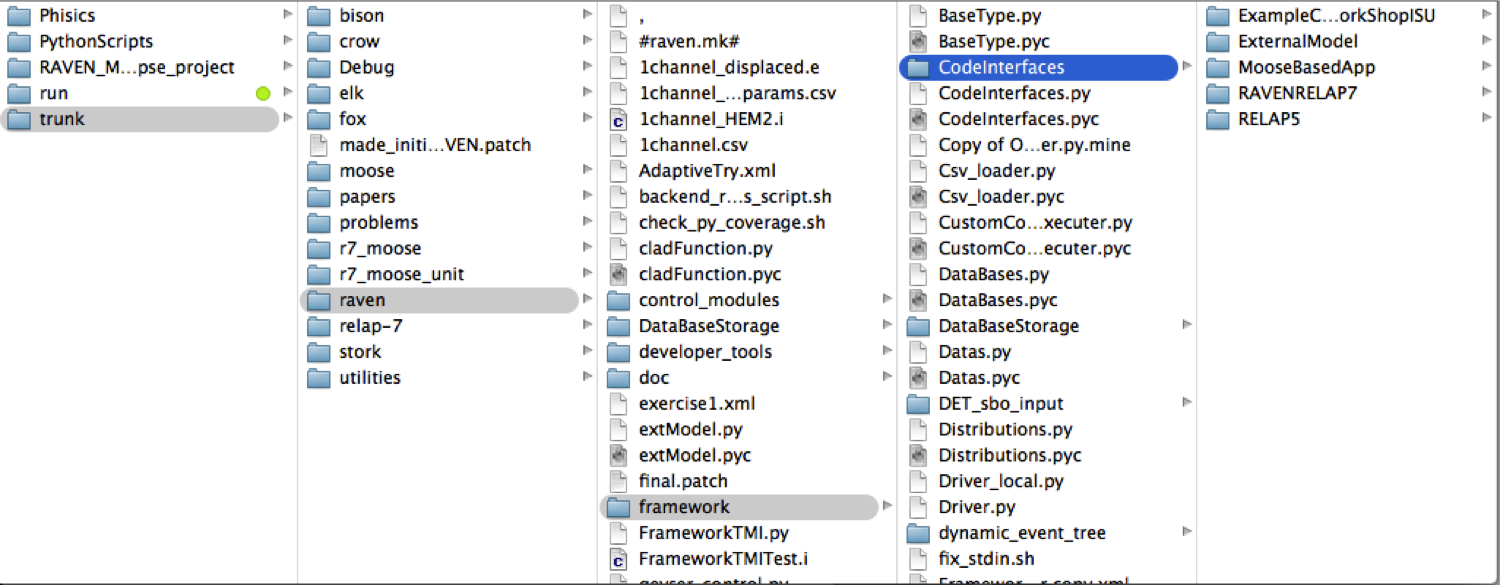
\includegraphics[width=1.0\textwidth]{pics/CodeInterfaceLocation.png}
\caption{Code Interface Location.}
\label{fig:codeinterface}
\end{figure}
The procedure of coupling a new code/application with RAVEN is quite a straightforward process. 
As for all the systems codes currently supported by RAVEN (e.g. RELAP-7, RELAP5-3D, 
BISON, MOOSE, etc.), the coupling is performed through a Python Interface that is in
 charge of interpreting the information coming from RAVEN and translating them in the
  input of the system code under consideration. 
\\The coupling procedure does not require to modify RAVEN itself. As already mentioned,
 the developer needs to create e new Python interface that is going to be embedded 
 in RAVEN at run-time (no need to introduce  hard-coded coupling statements). 
 This interface needs to be placed in a folder (whatever name) located in (see figure~\ref{fig:codeinterface}):
\begin{lstlisting}[language=bash]
 path_to_raven_distribution/raven/framework/CodeInterfaces/
\end{lstlisting}
At the initialization stage, RAVEN imports all the Interfaces that are contained in the directory above and performs some preliminary cross-checks.
In the following sub-sections, a step-by-step procedure is reported.
\subsection{Pre-requisites.} 
\label{subsec:prerequisites}
In order to couple a newer application to the RAVEN code, some (few) pre-requisites need to be satisfied.
%%% INPUT %%%
\newline
\\\textbf{\textit{\underline{Input}}}
\newline
\\ It would seem silly, but the first pre-requisite is the knowledge of the input 
syntax of the application the developer wants to couple. Indeed, RAVEN task
 ``ends'' at the Code Interface stage. RAVEN transfers the information needed 
 to perturb the input space into the Code interface and expects that the newly 
 developed Interface is able to perturb the input files based on the information 
 passed through.
\\This means that the developer needs to code a Python-compatible parser of
 the system code input (a module that is able to read and modify the input of 
 the particular code needs to be coupled).
\\ For example, let's suppose the input syntax of the code the developer needs 
to couple is as follows (simplest possible):
\begin{lstlisting}[language=python]
  kewword1 =  aValue1
  kewword2 =  aValue2
  kewword3 =  aValue3
  kewword4 =  aValue4
\end{lstlisting} 
The Python input parser would be as simple as:
\begin{lstlisting}[language=python]
class simpleInputParser():
  def __init__(self,filename):
    # 
    # @ In, string, filename, input file name (with path)
    #
    self.keywordDictionary = {}
    # open the file
    fileobject = open(filename)
    # store all the lines into a list
    lines = fileobject.readlines()
    # parse the list to construct 
    # self.keywordDictionary dictionary
    for line in lines:
      # split the line with respect
      # to the symbol "=" and store the
      # outcomes into the dictionary
      # listSplitted[0] is the keword
      # listSplitted[1] is the value
      listSplitted = line.split("=")
      keyword = listSplitted[0]
      value   = listSplitted[1]
      self.keywordDictionary[keyword] = value
    # close the file
    fileobject.close()
   
  def modifyInternalDictionary(self,inDictionary):
      # 
      # @ In, dictionary {keyword:value}, 
      # inDictionary, dictionary containing
      # the keywords to perturb 
      #

    # we just parse the dictionary and replace the
    # matching keywords
    for keyword,newvalue in inDictionary.items():
      self.keywordDictionary[keyword] = newvalue

  def writeNewInput(self,filename):
    #
    # @ In, string, filename, newer input file name (with path)
    #

    # open the file
    fileobject = open(filename)
    # write line by line
    for keyword,newvalue in self.keywordDictionary.items():
      fileobject.write(keyword + ``='' + str(newvalue) + ``\n'')
    # close the file
    fileobject.close()
\end{lstlisting} 
%%% OUTPUT %%%
\textbf{\textit{\underline{Output}}}
\newline
\\RAVEN is able to handle Comma Separated Value (CSV) files (as outputs 
of the system code). In order make RAVEN able to retrieve the information
 from the newly coupled code, these files need to be  either generate by the 
 system code itself or the developer needs to code a Python-compatible 
module to convert the whatever code output format to a CSV one. 
This module can be  directly called in the new code interface (see following section).
\\ Let's suppose that the output format of the code (the same of the previous 
input parser example) is as follows:
\begin{lstlisting}[language=python]
  result1 = aValue1
  result2 = aValue2
  result3 = aValue3
\end{lstlisting} 
The Python output converter would be as simple as:
\begin{lstlisting}[language=python]
def convertOutputFileToCSV(outputfile):
    keywordDictionary = {}
    # open the original file
    fileobject = open(outputfile)
    outputCSVfile = open (outputfile + '.csv')
    # store all the lines into a list
    lines = fileobject.readlines()
    # parse the list to construct 
    # self.keywordDictionary dictionary
    for line in lines:
      # split the line with respect
      # to the symbol "=" and store the
      # outcomes into the dictionary
      # listSplitted[0] is the keword
      # listSplitted[1] is the value
      listSplitted = line.split("=")
      keyword = listSplitted[0]
      value   = listSplitted[1]
      keywordDictionary[keyword] = value
    outputCSVfile.write(','.join(keywordDictionary.keys()))
    outputCSVfile.write(','.join(keywordDictionary.values()))
    outputCSVfile.close()
\end{lstlisting} 
And the output CSV becomes:
\begin{lstlisting}[language=python]
  result1, result2, result3
  aValue1, aValue2, aValue3 
\end{lstlisting} 
%%%%%%%
\subsection{Code Interface Creation} 
\label{subsec:codeinterfacecreation}
As already mentioned, RAVEN imports all the ``Code Interfaces'' at run-time, 
without actually knowing the syntax of the driven codes. In order to make RAVEN
able to drive a newer software, the developer needs to code a Python module 
that will contain few methods (with strict syntax) that are called by RAVEN during the simulation.
\\ When loading a ``Code Interface'', RAVEN expects to find, in the class representing the code,
 the following functions:
\begin{lstlisting}[language=python]
from CodeInterfaceBaseClass import CodeInterfaceBase
class NewCode(CodeInterfaceBase):
  def generateCommand(self, inputFiles, executable, flags = None)
  def createNewInput(self, currentInputFiles, oriInputFiles,
                                samplerType, **Kwargs)                           
  def finalizeCodeOutput(self, command, output, workingDir)
  def getInputExtension(self)
\end{lstlisting} 
In the following sub-sections all the methods are fully explained, providing examples
 (referring to the simple code used as example for the previous sections)
\subsubsection{Method: \textit{def generateCommand(self, inputFiles, executable)}} 
\label{subsubsec:generateCommand}
The \textbf{generateCommand} method is used to retrieve the command 
(in string format) needed to launch the driven Code and the root of the newer output (string).
 In other words, this 
method needs to return a string containing the full command 
that the internal JobHandler is going to use to run the Code this interface refers to. 
Hence, the return data type must be a TUPLE.
\\RAVEN is going to call this function passing in the following arguments:
\begin{itemize}
  \item \textbf{\textit{inputFiles}}, data type = list: List of input files (lenght of the list depends on the 
           number of inputs  have been added in the Step is running this code);
  \item \textbf{\textit{executable}} , data type = string, executable name with absolute 
            path \\(e.g. /home/path\_to\_executable/code.exe);
  \item  \textbf{\textit{flags}} , data type = string, a string containing the flags the 
               user can specify in the input (e.g. under the node $<Code><flags>-u -r</flags></Code>$).
\end{itemize}
For the example referred in the previous section, this method would be implemented as follows:
\newline
\begin{lstlisting}[language=python]
  def generateCommand(self,inputFiles,executable,flags=None):
    found = False
    for index, inputFile in enumerate(inputFiles):
      if inputFile.endswith(self.getInputExtension()):
        found = True
        break
    if not found: raise Exception(``NEWER CODE ERROR ->
                      None of the input files has one of the
                      following extensions ".i", ".inp"!'')
    outputfile = 'out~'+
       os.path.split(inputFiles[index])[1].split('.')[0]
    if flags: precommand = executable + flags
    else    : precommand = executable
    executeCommand = (precommand +
       `` -i '' +os.path.split(inputFiles[index])[1])
    return executeCommand,outputfile
\end{lstlisting} 
\subsubsection{Method: \textit{def createNewInput(self,currentInputFiles,
                                       \\oriInputFiles, samplerType,**Kwargs)}} 
\label{subsubsec:generateCommand}
The \textbf{createNewInput} method is used to generate an input based 
on the information RAVEN passes in. In this function the developer needs to 
call the driven code input parser in order to modify the input file, accordingly with
respect to the variables RAVEN is providing. This method needs to return a list containing 
the path and filenames of the modified input files. \nb RAVEN expects that at least one input 
file of the original list gets modified and re-named.
\\RAVEN is going to call this function passing in the following arguments:
\begin{itemize}
  \item \textbf{\textit{currentInputFiles}}, data type = list: List of current 
              input files (input files from last this method call);
  \item \textbf{\textit{oriInputFiles}} , data type = list, List of the original input files; 
  \item  \textbf{\textit{samplerType}} , data type = string, Sampler type (e.g. MonteCarlo,
               Adaptive, etc.). \nb None if no Sampler has been used;
  \item  \textbf{\textit{Kwargs}} , data type = kwarded dictionary, dictionary of parameters.
               In this dictionary there is another dictionary
               called "SampledVars" where RAVEN stores the 
               variables that got sampled 
               (Kwargs['SampledVars'] => {'var1':10,'var2':40});
\end{itemize}
For the example referred in the previous section, this method would implemented as follows:
\newline
\begin{lstlisting}[language=python]
  def createNewInput(self,currentInputFiles,
        oriInputFiles,samplerType,**Kwargs):
    for index, inputFile in enumerate(inputFiles):
      if inputFile.endswith(self.getInputExtension()):
        break
    parser = simpleInputParser(currentInputFiles[index])
    parser.modifyInternalDictionary(**Kwargs['SampledVars'])
    temp = str(oriInputFiles[index][:])
    newInputFiles = copy.copy(currentInputFiles)
    newInputFiles[index] = os.path.join(os.path.split(temp)[0],
           Kwargs['prefix']+"~"+os.path.split(temp)[1])
    parser.writeNewInput(newInputFiles[index])
    return newInputFiles
\end{lstlisting} 
\subsubsection{Method: \textit{getInputExtension(self, command, output, workingDir)}} 
\label{subsubsec:getInputExtension}
The \textbf{getInputExtension} function is an optional method. If present, it is called 
by RAVEN code at run time.  This function can be considered an utility method, since its
main goal is to return a tuple of strings, where the developer can place all the input extensions
the code interface needs to support (i.e. the extensions of the input(s) the code interface
is going to ``perturb''). If this method is not implemented, the default extensions are  \textbf{(``.i'',' ``.inp'', ``.in'')}.
This function does not accept any input argument.
For the example referred in the previous section, this method would implemented as follows:
\newline
\begin{lstlisting}[language=python]
def getInputExtension(self):
    return (``.i'',``.input'')
 \end{lstlisting} 
\subsubsection{Method: \textit{finalizeCodeOutput(self, command, output, workingDir)}} 
\label{subsubsec:finializeCodeOutput}
The \textbf{finalizeCodeOutput} function is an optional method. If present, it is called 
by RAVEN code at the end of each run. It can be used for those codes, that do not create CSV 
files as output to convert the whatever output format into a CSV. RAVEN checks if a string is returned; 
if so, RAVEN interprets that string as the new output file name (CSV).
\\RAVEN is going to call this function passing in the following arguments:
\begin{itemize}
  \item \textbf{\textit{command}}, data type = string: the command used to run 
                    the just ended job;
  \item \textbf{\textit{output}}, data type = string,the Output name root;
  \item  \textbf{\textit{workingDir}}, data type = string, current working directory.
\end{itemize}
For the example referred in the previous section, this method would implemented as follows:
\newline
\begin{lstlisting}[language=python]
def finalizeCodeOutput(self, command, output, workingDir)
    outfile = os.path.join(workingDir,output+'.o')
    outputobj=convertOutputFileToCSV(outfile)
 \end{lstlisting} 
 



\appendix
\section{Appendix: Example Primer}
\label{sec:examplePrimer}
In this Appendix, a set of examples are reported. In order to be as general as possible, the \textit{Model} type ``ExternalModel'' has been used.
%%%% EXAMPLE 1 
\subsection{Example 1.}
\label{subsec:ex1}
This simple example is about the construction of a ``Lorentz attractor'', sampling the relative input space. The parameters that are sampled represent the initial coordinate (x0,y0,z0) of the attractor origin. 

\begin{lstlisting}[style=XML,morekeywords={debug,re,seeding,class,subType,limit}]
<?xml version="1.0" encoding="UTF-8"?>
<Simulation verbosity="debug">
<!-- RUNINFO -->
<RunInfo>
    <WorkingDir>externalModel</WorkingDir>
    <Sequence>FirstMRun</Sequence>
    <batchSize>3</batchSize>
</RunInfo>
<!-- Files -->
<Files>
    <Input name='lorentzAttractor.py' type=''>lorentzAttractor</Input>
</Files>
<!-- STEPS -->
<Steps>
    <MultiRun name='FirstMRun'  re-seeding='25061978'>
        <Input   class='Files'     type=''               >lorentzAttractor.py</Input>
        <Model   class='Models'    type='ExternalModel'  >PythonModule</Model>
        <Sampler class='Samplers'  type='MonteCarlo'     >MC_external</Sampler>
        <Output  class='DataObjects'     type='HistorySet'      >testPrintHistorySet</Output>
        <Output  class='Databases' type='HDF5'           >test_external_db</Output>
        <Output  class='OutStreamManager' type='Print'   >testPrintHistorySet_dump</Output>
    </MultiRun >
</Steps>
<!-- MODELS -->
<Models>
    <ExternalModel name='PythonModule' subType='' ModuleToLoad='externalModel/lorentzAttractor'>  
       <variable>sigma</variable>
       <variable>rho</variable>
       <variable>beta</variable>
       <variable>x</variable>
       <variable>y</variable>
       <variable>z</variable>
       <variable>time</variable>
       <variable>x0</variable>
       <variable>y0</variable>
       <variable>z0</variable>
    </ExternalModel>
</Models>
<!-- DISTRIBUTIONS -->
<Distributions>
    <Normal name='x0_distrib'>
        <mean>4</mean>
        <sigma>1</sigma>
    </Normal>
    <Normal name='y0_distrib'>
        <mean>4</mean>
        <sigma>1</sigma>
    </Normal>
    <Normal name='z0_distrib'>
        <mean>4</mean>
        <sigma>1</sigma>
    </Normal>
</Distributions>
<!-- SAMPLERS -->
<Samplers>
    <MonteCarlo name='MC_external'>
      <sampler_init>
        <limit>3</limit>
      </sampler_init>
      <variable name='x0' >
        <distribution  >x0_distrib</distribution>
      </variable>
      <variable name='y0' >
        <distribution  >y0_distrib</distribution>
      </variable>
      <variable name='z0' >
        <distribution  >z0_distrib</distribution>
      </variable>
    </MonteCarlo>
</Samplers>
<!-- DATABASES -->
<Databases>
  <HDF5 name="test_external_db"/>
</Databases>
<!-- OUTSTREAMS -->
<OutStreamManager>
  <Print name='testPrintHistorySet_dump'>
    <type>csv</type>
    <source>testPrintHistorySet</source>
  </Print>
</OutStreamManager>
<!-- DATA OBJECTS -->
<DataObjects>
    <HistorySet name='testPrintHistorySet'>
        <Input>x0,y0,z0</Input>
        <Output>time,x,y,z</Output>
   </HistorySet>
</DataObjects>
</Simulation>
\end{lstlisting}
The Python \textit{ExternalModel} is reported below:
\begin{lstlisting}[language=python]
import numpy as np

def run(self,Input):
  max_time = 0.03
  t_step = 0.01

  numberTimeSteps = int(max_time/t_step)

  self.x = np.zeros(numberTimeSteps)
  self.y = np.zeros(numberTimeSteps)
  self.z = np.zeros(numberTimeSteps)
  self.time = np.zeros(numberTimeSteps)

  self.x0 = Input['x0']
  self.y0 = Input['y0']
  self.z0 = Input['z0']

  self.x[0] = Input['x0']
  self.y[0] = Input['y0']
  self.z[0] = Input['z0']
  self.time[0]= 0

  for t in range (numberTimeSteps-1):
    self.time[t+1] = self.time[t] + t_step
    self.x[t+1]    = self.x[t] +  self.sigma*
                      (self.y[t]-self.x[t]) * t_step
    self.y[t+1]    = self.y[t] + (self.x[t]*
                      (self.rho-self.z[t])-self.y[t]) * t_step
    self.z[t+1]    = self.z[t] + (self.x[t]*
                          self.y[t]-self.beta*self.z[t]) * t_step
\end{lstlisting}
%%%% EXAMPLE 2 
\subsection{Example 2.}
\label{subsec:ex1}
This example shows a slightly more complicated example, that employs the usage of:
\begin{itemize}
    \item \textit{Samplers:} Grid and Adaptive;
    \item \textit{Models:} External, Reduce Order Models and Post-Processors;
    \item \textit{OutStreams:} Prints and Plots;
    \item \textit{Data Objects:} PointSets;
    \item \textit{Functions:} ExternalFunctions.
\end{itemize}
The goal of this input is to compute the ``SafestPoint''.
It provides the coordinates of the farthest
point from the limit surface that is given as an input.
%
The safest point coordinates are expected values of the coordinates of the
farthest points from the limit surface in the space of the ``controllable''
variables based on the probability distributions of the ``non-controllable''
variables.

The term ``controllable'' identifies those variables that are under control
during the system operation, while the ``non-controllable'' variables are
stochastic parameters affecting the system behaviour randomly.

The ``SafestPoint'' post-processor requires the set of points belonging to the
limit surface, which must be given as an input.

\begin{lstlisting}[style=XML,morekeywords={debug,re,seeding,class,subType,limit}]
<Simulation verbosity='debug'>

<!-- RUNINFO -->
<RunInfo>
  <WorkingDir>SafestPointPP</WorkingDir>
  <Sequence>pth1,pth2,pth3,pth4</Sequence>
  <batchSize>50</batchSize>
</RunInfo>

<!-- STEPS -->
<Steps>  
  <MultiRun name = 'pth1' pauseAtEnd = 'False'>
    <Sampler  class = 'Samplers'  type = 'Grid'           >grd_vl_ql_smp_dpt</Sampler>
    <Input    class = 'DataObjects'     type = 'PointSet'   >grd_vl_ql_smp_dpt_dt</Input>
    <Model    class = 'Models'    type = 'ExternalModel'  >xtr_mdl</Model>
    <Output   class = 'DataObjects'     type = 'PointSet'   >nt_phy_dpt_dt</Output>    
  </MultiRun >
  
  <MultiRun name = 'pth2' pauseAtEnd = 'True'>
    <Sampler          class = 'Samplers'  type = 'Adaptive'      >dpt_smp</Sampler>
    <Input            class = 'DataObjects'     type = 'PointSet'  >bln_smp_dt</Input>   
    <Model            class = 'Models'    type = 'ExternalModel' >xtr_mdl</Model>
    <Output           class = 'DataObjects'     type = 'PointSet'  >nt_phy_dpt_dt</Output>            
    <SolutionExport   class = 'DataObjects'     type = 'PointSet'  >lmt_srf_dt</SolutionExport>
  </MultiRun>
  
  <PostProcess name='pth3' pauseAtEnd = 'False'>
    <Input    class = 'DataObjects'          type = 'PointSet'       >lmt_srf_dt</Input>
    <Model    class = 'Models'         type = 'PostProcessor'  >SP</Model>
    <Output   class = 'DataObjects'          type = 'PointSet'     >sfs_pnt_dt</Output>
  </PostProcess>  
  
  <OutStreamStep name = 'pth4' pauseAtEnd = 'True'>
  	<Input  class = 'DataObjects'            type = 'PointSet'  >lmt_srf_dt</Input>
  	<Output class = 'OutStreamManager' type = 'Print'         >lmt_srf_dmp</Output>
    <Input  class = 'DataObjects'            type = 'PointSet'  >sfs_pnt_dt</Input>
  	<Output class = 'OutStreamManager' type = 'Print'         >sfs_pnt_dmp</Output>
  </OutStreamStep>
</Steps>

<!-- DATA OBJECTS -->
<DataObjects> 
  <PointSet name = 'grd_vl_ql_smp_dpt_dt'>
    <Input>x1,x2,gammay</Input>
    <Output>OutputPlaceHolder</Output>
  </PointSet>
  
  <PointSet name = 'nt_phy_dpt_dt'>
    <Input>x1,x2,gammay</Input>
    <Output>g</Output>
  </PointSet>
    
  <PointSet name = 'bln_smp_dt'>
    <Input>x1,x2,gammay</Input>
    <Output>OutputPlaceHolder</Output>
  </PointSet>
    
  <PointSet name = 'lmt_srf_dt'>
    <Input>x1,x2,gammay</Input>
    <Output>g_zr</Output>
  </PointSet>
  
  <PointSet name = 'sfs_pnt_dt'>
    <Input>x1,x2,gammay</Input>
    <Output>p</Output>
  </PointSet>
</DataObjects>

<!-- DISTRIBUTIONS -->
<Distributions>
  <Normal name = 'x1_dst'>
    <upperBound>10</upperBound>
    <lowerBound>-10</lowerBound>
  	<mean>0.5</mean>
    <sigma>0.1</sigma>
  </Normal>
  
  <Normal name = 'x2_dst'>
    <upperBound>10</upperBound>
    <lowerBound>-10</lowerBound>
    <mean>-0.15</mean>
    <sigma>0.05</sigma>
  </Normal>
  
  <Normal name = 'gammay_dst'>
    <upperBound>20</upperBound>
    <lowerBound>-20</lowerBound>
    <mean>0</mean>
    <sigma>15</sigma>
  </Normal>
</Distributions>

<!-- SAMPLERS -->
<Samplers>  
  <Grid name = 'grd_vl_ql_smp_dpt'>
    <variable name = 'x1' >
      <distribution>x1_dst</distribution>
      <grid type = 'value' construction = 'equal' steps = '10' upperBound = '10'>2</grid>
    </variable>  
    <variable name='x2' >
      <distribution>x2_dst</distribution>
      <grid type = 'value' construction = 'equal' steps = '10' upperBound = '10'>2</grid>
    </variable>
    <variable name='gammay' >
      <distribution>gammay_dst</distribution>
      <grid type = 'value' construction = 'equal' steps = '10' lowerBound = '-20'>4</grid>
    </variable>
  </Grid>
  
  <Adaptive name = 'dpt_smp' verbosity='debug'>
    <ROM              class = 'Models'    type = 'ROM'           >accelerated_ROM</ROM>
    <Function         class = 'Functions' type = 'External'      >g_zr</Function>
    <TargetEvaluation class = 'DataObjects'     type = 'PointSet'  >nt_phy_dpt_dt</TargetEvaluation>
    <Convergence limit = '3000' forceIteration = 'False' weight = 'none' persistence = '5'>1e-2</Convergence>
      <variable name = 'x1'>
        <distribution>x1_dst</distribution>
      </variable>
      <variable name = 'x2'>
        <distribution>x2_dst</distribution>
      </variable>
      <variable name = 'gammay'>
        <distribution>gammay_dst</distribution>
      </variable>
  </Adaptive>
</Samplers>

<!-- MODELS -->
<Models>  
  <ExternalModel name = 'xtr_mdl' subType = '' ModuleToLoad = 'SafestPointPP/safest_point_test_xtr_mdl'>
    <variable>x1</variable>
    <variable>x2</variable>
    <variable>gammay</variable>
    <variable>g</variable>
  </ExternalModel>
  
  <ROM name = 'accelerated_ROM' subType = 'SciKitLearn'>
    <Features>x1,x2,gammay</Features>
    <Target>g_zr</Target>
    <SKLtype>svm|SVC</SKLtype>
    <kernel>rbf</kernel>
    <gamma>10</gamma>
    <tol>1e-5</tol>
    <C>50</C>
  </ROM>

  <PostProcessor name='SP' subType='SafestPoint'>
    <!-- List of Objects (external with respect to this PP) needed by this post-processor -->
    <Distribution     class = 'Distributions'  type = 'Normal'>x1_dst</Distribution>
    <Distribution     class = 'Distributions'  type = 'Normal'>x2_dst</Distribution>
    <Distribution     class = 'Distributions'  type = 'Normal'>gammay_dst</Distribution>
    <!- end of the list -->
    <controllable>
    	<variable name = 'x1'>
    		<distribution>x1_dst</distribution>
    		<grid type = 'value' steps = '20'>1</grid>   		
    	</variable>
    	<variable name = 'x2'>
    		<distribution>x2_dst</distribution>
    		<grid type = 'value' steps = '20'>1</grid>   		
    	</variable>
    </controllable>
    <non-controllable>
    	<variable name = 'gammay'>
    		<distribution>gammay_dst</distribution>
    		<grid type = 'value' steps = '20'>2</grid>
    	</variable> 	
    </non-controllable>
  </PostProcessor>
</Models>

<!-- FUNCTIONS -->
<Functions>
  <External name='g_zr' file='SafestPointPP/safest_point_test_g_zr.py'>
    <variable>g</variable>
  </External>
</Functions>

<!-- OUT-STREAMS -->
<OutStreamManager> 
  <Print name = 'lmt_srf_dmp'>
  	<type>csv</type>
  	<source>lmt_srf_dt</source>
  </Print>
  
  <Print name = 'sfs_pnt_dmp'>
  	<type>csv</type>
  	<source>sfs_pnt_dt</source>
  </Print>
</OutStreamManager>

</Simulation>
\end{lstlisting}
The Python \textit{ExternalModel} is reported below:
\begin{lstlisting}[language=python]
def run(self,Input): 
  self.g = self.x1+4*self.x2-self.gammay
\end{lstlisting}
The ``Goal Function'',the function that defines the transitions with respect the input space coordinates, is as follows:
\begin{lstlisting}[language=python]
def __residuumSign(self):
  if self.g<0 : return  1
  else        : return -1
\end{lstlisting}

%%%%% EXAMPLE 3
%\subsection{Example3}
%\label{subsec:ex1}
%example 3



    % ---------------------------------------------------------------------- %
    % References
    %
    \clearpage
    % If hyperref is included, then \phantomsection is already defined.
    % If not, we need to define it.
    \providecommand*{\phantomsection}{}
    \phantomsection
    \addcontentsline{toc}{section}{References}
    \bibliographystyle{ieeetr}
    \bibliography{raven_user_manual}


    % ---------------------------------------------------------------------- %
    %

    % \printindex

    %\include{distribution}

\end{document}
